%%%%%%%%%%%%%%%%%%%%%%%%%%%%%%%%%%%%%%%%%%%%%%%%%%%%%%%%%%%%%%%
%% OXFORD THESIS TEMPLATE

% Use this template to produce a standard thesis that meets the Oxford University requirements for DPhil submission
%
% Originally by Keith A. Gillow (gillow@maths.ox.ac.uk), 1997
% Modified by Sam Evans (sam@samuelevansresearch.org), 2007
% Modified by John McManigle (john@oxfordechoes.com), 2015
% Modified by Ulrik Lyngs (ulrik.lyngs@cs.ox.ac.uk), 2018, for use with R Markdown
%
% Ulrik Lyngs, 25 Nov 2018: Following John McManigle, broad permissions are granted to use, modify, and distribute this software
% as specified in the MIT License included in this distribution's LICENSE file.
%
% John tried to comment this file extensively, so read through it to see how to use the various options.  Remember
% that in LaTeX, any line starting with a % is NOT executed.  Several places below, you have a choice of which line to use
% out of multiple options (eg draft vs final, for PDF vs for binding, etc.)  When you pick one, add a % to the beginning of
% the lines you don't want.


%%%%% CHOOSE PAGE LAYOUT
% The most common choices should be below.  You can also do other things, like replacing "a4paper" with "letterpaper", etc.

% This one will format for two-sided binding (ie left and right pages have mirror margins; blank pages inserted where needed):
%\documentclass[a4paper,twoside]{templates/ociamthesis}
% This one will format for one-sided binding (ie left margin > right margin; no extra blank pages):
%\documentclass[a4paper]{ociamthesis}
% This one will format for PDF output (ie equal margins, no extra blank pages):
%\documentclass[a4paper,nobind]{templates/ociamthesis}
%UL 2 Dec 2018: pass this in from YAML

\documentclass[a4paper, twoside]{templates/ociamthesis}

\usepackage{float}

% Allows for kableExtra to keep table footnotes/etc same width as table
\usepackage{booktabs}
\usepackage{threeparttable}
\usepackage{threeparttablex}

% Enable use of landscape for tables
\usepackage{lscape}
\newcommand{\blandscape}{\begin{landscape}}
\newcommand{\elandscape}{\end{landscape}}

% Loading this package ensures that the blank pages used to ensure chapters start on right do not have headers/footers
\usepackage{emptypage}

% UL 30 Nov 2018 pandoc puts lists in 'tightlist' command when no space between bullet points in Rmd file
\providecommand{\tightlist}{%
  \setlength{\itemsep}{0pt}\setlength{\parskip}{0pt}}
 
% UL 1 Dec 2018, fix to include code in shaded environments
\usepackage{color}
\usepackage{fancyvrb}
\newcommand{\VerbBar}{|}
\newcommand{\VERB}{\Verb[commandchars=\\\{\}]}
\DefineVerbatimEnvironment{Highlighting}{Verbatim}{commandchars=\\\{\}}
% Add ',fontsize=\small' for more characters per line
\usepackage{framed}
\definecolor{shadecolor}{RGB}{248,248,248}
\newenvironment{Shaded}{\begin{snugshade}}{\end{snugshade}}
\newcommand{\AlertTok}[1]{\textcolor[rgb]{0.94,0.16,0.16}{#1}}
\newcommand{\AnnotationTok}[1]{\textcolor[rgb]{0.56,0.35,0.01}{\textbf{\textit{#1}}}}
\newcommand{\AttributeTok}[1]{\textcolor[rgb]{0.77,0.63,0.00}{#1}}
\newcommand{\BaseNTok}[1]{\textcolor[rgb]{0.00,0.00,0.81}{#1}}
\newcommand{\BuiltInTok}[1]{#1}
\newcommand{\CharTok}[1]{\textcolor[rgb]{0.31,0.60,0.02}{#1}}
\newcommand{\CommentTok}[1]{\textcolor[rgb]{0.56,0.35,0.01}{\textit{#1}}}
\newcommand{\CommentVarTok}[1]{\textcolor[rgb]{0.56,0.35,0.01}{\textbf{\textit{#1}}}}
\newcommand{\ConstantTok}[1]{\textcolor[rgb]{0.00,0.00,0.00}{#1}}
\newcommand{\ControlFlowTok}[1]{\textcolor[rgb]{0.13,0.29,0.53}{\textbf{#1}}}
\newcommand{\DataTypeTok}[1]{\textcolor[rgb]{0.13,0.29,0.53}{#1}}
\newcommand{\DecValTok}[1]{\textcolor[rgb]{0.00,0.00,0.81}{#1}}
\newcommand{\DocumentationTok}[1]{\textcolor[rgb]{0.56,0.35,0.01}{\textbf{\textit{#1}}}}
\newcommand{\ErrorTok}[1]{\textcolor[rgb]{0.64,0.00,0.00}{\textbf{#1}}}
\newcommand{\ExtensionTok}[1]{#1}
\newcommand{\FloatTok}[1]{\textcolor[rgb]{0.00,0.00,0.81}{#1}}
\newcommand{\FunctionTok}[1]{\textcolor[rgb]{0.00,0.00,0.00}{#1}}
\newcommand{\ImportTok}[1]{#1}
\newcommand{\InformationTok}[1]{\textcolor[rgb]{0.56,0.35,0.01}{\textbf{\textit{#1}}}}
\newcommand{\KeywordTok}[1]{\textcolor[rgb]{0.13,0.29,0.53}{\textbf{#1}}}
\newcommand{\NormalTok}[1]{#1}
\newcommand{\OperatorTok}[1]{\textcolor[rgb]{0.81,0.36,0.00}{\textbf{#1}}}
\newcommand{\OtherTok}[1]{\textcolor[rgb]{0.56,0.35,0.01}{#1}}
\newcommand{\PreprocessorTok}[1]{\textcolor[rgb]{0.56,0.35,0.01}{\textit{#1}}}
\newcommand{\RegionMarkerTok}[1]{#1}
\newcommand{\SpecialCharTok}[1]{\textcolor[rgb]{0.00,0.00,0.00}{#1}}
\newcommand{\SpecialStringTok}[1]{\textcolor[rgb]{0.31,0.60,0.02}{#1}}
\newcommand{\StringTok}[1]{\textcolor[rgb]{0.31,0.60,0.02}{#1}}
\newcommand{\VariableTok}[1]{\textcolor[rgb]{0.00,0.00,0.00}{#1}}
\newcommand{\VerbatimStringTok}[1]{\textcolor[rgb]{0.31,0.60,0.02}{#1}}
\newcommand{\WarningTok}[1]{\textcolor[rgb]{0.56,0.35,0.01}{\textbf{\textit{#1}}}}
%UL 2 Dec 2018 add a bit of white space before and after code blocks
\renewenvironment{Shaded}
{
  \vspace{4pt}%
  \begin{snugshade}%
}{%
  \end{snugshade}%
  \vspace{4pt}%
}

%UL 2 Dec 2018 reduce whitespace around verbatim environments
\usepackage{etoolbox}
\makeatletter
\preto{\@verbatim}{\topsep=0pt \partopsep=0pt }
\makeatother

%UL 26 Mar 2019, enable strikethrough
\usepackage[normalem]{ulem}

%UL 15 Oct 2019, enable link highlighting to be turned off from YAML
\usepackage[colorlinks=false,pdfpagelabels,hidelinks=true]{hyperref}

%%%%% SELECT YOUR DRAFT OPTIONS
% Three options going on here; use in any combination.  But remember to turn the first two off before
% generating a PDF to send to the printer!

% This adds a "DRAFT" footer to every normal page.  (The first page of each chapter is not a "normal" page.)

% This highlights (in blue) corrections marked with (for words) \mccorrect{blah} or (for whole
% paragraphs) \begin{mccorrection} . . . \end{mccorrection}.  This can be useful for sending a PDF of
% your corrected thesis to your examiners for review.  Turn it off, and the blue disappears.
\correctionstrue

%%%%% BIBLIOGRAPHY SETUP
% Note that your bibliography will require some tweaking depending on your department, preferred format, etc.
% The options included below are just very basic "sciencey" and "humanitiesey" options to get started.
% If you've not used LaTeX before, I recommend reading a little about biblatex/biber and getting started with it.
% If you're already a LaTeX pro and are used to natbib or something, modify as necessary.
% Either way, you'll have to choose and configure an appropriate bibliography format...

% The science-type option: numerical in-text citation with references in order of appearance.
% \usepackage[style=numeric-comp, sorting=none, backend=biber, doi=false, isbn=false]{biblatex}
% \newcommand*{\bibtitle}{References}

% The humanities-type option: author-year in-text citation with an alphabetical works cited.
% \usepackage[style=authoryear, sorting=nyt, backend=biber, maxcitenames=2, useprefix, doi=false, isbn=false]{biblatex}
% \newcommand*{\bibtitle}{Works Cited}



%UL 3 Dec 2018: set this from YAML in index.Rmd
\usepackage[style=numeric-comp, sorting=none, backend=biber, doi=true, isbn=false]{biblatex}
\newcommand*{\bibtitle}{Bibliography}

% Change this to the name of your .bib file (usually exported from a citation manager like Zotero or EndNote).
\addbibresource{bibliography/references.bib}

% Add definition of CSLReferences section to allow for compatibility with new pan
\newlength{\cslhangindent}
\setlength{\cslhangindent}{1.5em}
\newlength{\csllabelwidth}
\setlength{\csllabelwidth}{3em}
\newenvironment{CSLReferences}[3] % #1 hanging-ident, #2 entry spacing
 {% don't indent paragraphs
  \setlength{\parindent}{0pt}
  % turn on hanging indent if param 1 is 1
  \ifodd #1 \everypar{\setlength{\hangindent}{\cslhangindent}}\ignorespaces\fi
  % set entry spacing
  \ifnum #2 > 0
  \setlength{\parskip}{#2\baselineskip}
  \fi
 }%
 {}
\usepackage{calc} % for \widthof, \maxof
\newcommand{\CSLBlock}[1]{#1\hfill\break}
\newcommand{\CSLLeftMargin}[1]{\parbox[t]{\maxof{\widthof{#1}}{\csllabelwidth}}{#1}}
\newcommand{\CSLRightInline}[1]{\parbox[t]{\linewidth - \csllabelwidth}{#1}}
\newcommand{\CSLIndent}[1]{\hspace{\cslhangindent}#1}

% Uncomment this if you want equation numbers per section (2.3.12), instead of per chapter (2.18):
%\numberwithin{equation}{subsection}

%%%%% THESIS / TITLE PAGE INFORMATION
% Everybody needs to complete the following:
\title{Determining the causal effects of lipid levels on risk of dementia:\\
a triangulation of new and existing evidence}
\author{Luke A McGuinness}
\college{}

% Master's candidates who require the alternate title page (with candidate number and word count)
% must also un-comment and complete the following three lines:
%\masterssubmissiontrue
%\candidateno{933516}
%\wordcount{28,815}

% Uncomment the following line if your degree also includes exams (eg most masters):
%\renewcommand{\submittedtext}{Submitted in partial completion of the}
% Your full degree name.  (But remember that DPhils aren't "in" anything.  They're just DPhils.)
\degree{Doctor of Philosophy}
% Term and year of submission, or date if your board requires (eg most masters)
\degreedate{2022}
\wordcount{40977}


%%%%% YOUR OWN PERSONAL MACROS
% This is a good place to dump your own LaTeX macros as they come up.

% To make text superscripts shortcuts
	\renewcommand{\th}{\textsuperscript{th}} % ex: I won 4\th place
	\newcommand{\nd}{\textsuperscript{nd}}
	\renewcommand{\st}{\textsuperscript{st}}
	\newcommand{\rd}{\textsuperscript{rd}}
	
	\definecolor{ashgray}{rgb}{0.7,0.75,0.71}
	
%%%%% THE ACTUAL DOCUMENT STARTS HERE
\begin{document}

%%%%% CHOOSE YOUR LINE SPACING HERE
% This is the official option.  Use it for your submission copy and library copy:
\setlength{\textbaselineskip}{22pt plus2pt}
% This is closer spacing (about 1.5-spaced) that you might prefer for your personal copies:
%\setlength{\textbaselineskip}{18pt plus2pt minus1pt}

% You can set the spacing here for the roman-numbered pages (acknowledgements, table of contents, etc.)
\setlength{\frontmatterbaselineskip}{17pt plus1pt minus1pt}

% UL: You can set the line and paragraph spacing here for the separate abstract page to be handed in to Examination schools
\setlength{\abstractseparatelineskip}{13pt plus1pt minus1pt}
\setlength{\abstractseparateparskip}{0pt plus 1pt}

% UL: You can set the general paragraph spacing here - I've set it to 2pt (was 0) so
% it's less claustrophobic
\setlength{\parskip}{6pt plus 1pt}


% Leave this line alone; it gets things started for the real document.
\setlength{\baselineskip}{\textbaselineskip}


%%%%% CHOOSE YOUR SECTION NUMBERING DEPTH HERE
% You have two choices.  First, how far down are sections numbered?  (Below that, they're named but
% don't get numbers.)  Second, what level of section appears in the table of contents?  These don't have
% to match: you can have numbered sections that don't show up in the ToC, or unnumbered sections that
% do.  Throughout, 0 = chapter; 1 = section; 2 = subsection; 3 = subsubsection, 4 = paragraph...

% The level that gets a number:
\setcounter{secnumdepth}{2}
% The level that shows up in the ToC:
\setcounter{tocdepth}{2}
% The level that shows up in the mini-ToC:
\setcounter{minitocdepth}{1} 

%%%%% ABSTRACT SEPARATE
% This is used to create the separate, one-page abstract that you are required to hand into the Exam
% Schools.  You can comment it out to generate a PDF for printing or whatnot.
\begin{abstractseparate}
  \textbf{Background}\\
  In the UK, an estimated 800000 people are currently living with dementia and this number is expected to double
  by 2040. Despite the number of dementia cases and decades of research, there remains much unknown about
  the pathogenesis and progression of the disease, and, at present, no effective treatment exists to arrest or
  reverse the cognitive decline associated with the condition. In this context, identification of causal relationships
  between modifiable targets and dementia risk is central to the development of evidence-based prevention
  strategies and will be critically important in maintaining the long-term health of the ageing public. Blood lipid
  levels have been implicated in the aetiology of dementia by genetic linkage and functional cell biology studies,
  but current epidemiological evidence has yet to reach a consensus on their role in dementia risk.
\end{abstractseparate}

% JEM: Pages are roman numbered from here, though page numbers are invisible until ToC.  This is in
% keeping with most typesetting conventions.
\begin{romanpages}

% Title page is created here
\maketitle

%%%%% ABSTRACT -- Nothing to do here except comment out if you don't want it.
\begin{abstract}
	\textbf{Background}\\
 In the UK, an estimated 800000 people are currently living with dementia and this number is expected to double
 by 2040. Despite the number of dementia cases and decades of research, there remains much unknown about
 the pathogenesis and progression of the disease, and, at present, no effective treatment exists to arrest or
 reverse the cognitive decline associated with the condition. In this context, identification of causal relationships
 between modifiable targets and dementia risk is central to the development of evidence-based prevention
 strategies and will be critically important in maintaining the long-term health of the ageing public. Blood lipid
 levels have been implicated in the aetiology of dementia by genetic linkage and functional cell biology studies,
 but current epidemiological evidence has yet to reach a consensus on their role in dementia risk.
\end{abstract}

%%%%% DEDICATION -- If you'd like one, un-comment the following.
\begin{dedication}
  For Brendan McHugh
\end{dedication}

%%%%% ACKNOWLEDGEMENTS -- Nothing to do here except comment out if you don't want it.
\begin{acknowledgements}
 	\textbf{Professional}

  There are so many people without whom this would not have been possible:

  {[}\textbf{Check all name spellings}{]}

  Sharen O'Keffe
  Neal Haddaway
  Martin Westgate

  Emily Hennessy

  robvis contributors: (there are at least 3)

  Annual reviewers: Rupert Payne and Emma Anderson

  Those who contributed their time to dual marking papers and code with me,

  Thanks to Francesca for sharing advance copy of review of Mendelian randomisation studies, to inform choice of tool.

  I am a NIHR Doctoral Research Fellow with grant code \textbf{TBC}. The funding source had no role in the design, conduct of the study, collection, management, analysis and interpretation or preparation, review, or approval of the thesis.

  Thanks also to all those who raised issues or otherwise provided feedback on the open source tools built as part of this thesis:
  \href{https://github.com/abannachbrown}{@abannachbrown}, \href{https://github.com/ailengt}{@ailengt}, \href{https://github.com/AJFOWLER}{@AJFOWLER}, \href{https://github.com/danielskatz}{@danielskatz}, \href{https://github.com/earcanal}{@earcanal}, \href{https://github.com/Jamesohare1}{@Jamesohare1}, \href{https://github.com/jannisborn}{@jannisborn}, \href{https://github.com/paulsharpeY}{@paulsharpeY}, \href{https://github.com/rachaelmburke}{@rachaelmburke}, \href{https://github.com/rdboyes}{@rdboyes}, \href{https://github.com/seabbs}{@seabbs}, \href{https://github.com/vanAmsterdam}{@vanAmsterdam}, \href{https://github.com/yochannah}{@yochannah}, and \href{https://github.com/zaddyzad}{@zaddyzad}.

  Statistical support: check emails!

  All authors who volunteered time and effort to provided

  A special thanks goes out to Mark Newbury of the

  My student, Georgia Gourlay

  \textbf{Personal}

  Finally, thanks to parents and Ciara Gardiner.

  \begin{flushright}
  Canynge Hall, Bristol \\1 December 2021
  \end{flushright}
\end{acknowledgements}

%%%%% DECALRATION -- Nothing to do here except comment out if you don't want it.
\begin{declaration}
 	I declare that the work in this dissertation was carried out in accordance with the requirements of the University's Regulations and Code of Practice for Research Degree Programmes and that it has not been submitted for any other academic award. Except where indicated by specific reference in the text, the work is the candidate's own work. Work done in collaboration with, or with the assistance of, others, is indicated as such. Any views expressed in the dissertation are those of the author.

  \begin{flushright}
  SIGNED: .............................................................         DATE: ..........................\\
  \end{flushright}
\end{declaration}

%%%%% COVID Statement -- Nothing to do here except comment out if you don't want it.
\begin{covidStatment}
 	My work was influence by COVID in the following ways:
\end{covidStatment}

%%%%% MINI TABLES
% This lays the groundwork for per-chapter, mini tables of contents.  Comment the following line
% (and remove \minitoc from the chapter files) if you don't want this.  Un-comment either of the
% next two lines if you want a per-chapter list of figures or tables.
  \dominitoc % include a mini table of contents

% This aligns the bottom of the text of each page.  It generally makes things look better.
\flushbottom

% This is where the whole-document ToC appears:
\tableofcontents

\listoffigures
	\mtcaddchapter
  	% \mtcaddchapter is needed when adding a non-chapter (but chapter-like) entity to avoid confusing minitoc

% Uncomment to generate a list of tables:
\listoftables
  \mtcaddchapter
%%%%% LIST OF ABBREVIATIONS
% This example includes a list of abbreviations.  Look at text/abbreviations.tex to see how that file is
% formatted.  The template can handle any kind of list though, so this might be a good place for a
% glossary, etc.
% First parameter can be changed eg to "Glossary" or something.
% Second parameter is the max length of bold terms.
\begin{mclistof}{List of Abbreviations}{3.2cm}

\item[1-D, 2-D] One- or two-dimensional, referring in this thesis to spatial dimensions in an image.

\item[Otter] One of the finest of water mammals.

\item[Hedgehog] Quite a nice prickly friend.

\end{mclistof} 


% The Roman pages, like the Roman Empire, must come to its inevitable close.
\end{romanpages}

%%%%% CHAPTERS
% Add or remove any chapters you'd like here, by file name (excluding '.tex'):
\flushbottom

% all your chapters and appendices will appear here
\hypertarget{covering-material}{%
\chapter*{Covering material}\label{covering-material}}
\addcontentsline{toc}{chapter}{Covering material}

\adjustmtc

Word count: 41048

Table words: 3487

Days: 355

Words behind: 1033

Words today: 608

~

~

\includegraphics{_main_files/figure-latex/wordcount-fig-1.pdf}



\hypertarget{background-heading}{%
\chapter{Background, Theoretical framework, Aims \& Objectives}\label{background-heading}}

\minitoc 

\hypertarget{lay-summary}{%
\section{Lay summary}\label{lay-summary}}

Around 850,000 people in the UK live with dementia, and by 2040, nearly twice as many will have the condition. Despite many promising candidates, no cure for dementia currently exists, meaning the focus is on finding ways to prevent the condition. The best way to do this is to find risk factors (characteristics that influence a person's chance of developing a disease) for dementia that we can easily change. Avoiding a risk factor does not guarantee that a person will not develop dementia but makes it less likely. A key risk factor for dementia may be the levels of lipids (fatty substances such as cholesterol) in a person's blood, though not all existing research agrees. The aim of this thesis is to use all available evidence to assess whether blood lipids levels are in fact a risk factor for dementia.

This introductory chapter provides background information on both dementia and blood lipids, and on the potential link between them. It introduces the theory used to frame the research presented here, and then maps the formal aims and objectives of the research project to the relevant chapters of this thesis. Finally, it summarises the outputs (journal articles, presentations and software) that were created as part of this thesis.

\hypertarget{introduction}{%
\section{Introduction}\label{introduction}}

This chapter provides an overview of the broad context of this thesis, introducing the core concepts used throughout and providing some background on each. It briefly discusses the underlying pathologies and diagnosis of dementia, its public health importance, and the current state of treatment and prevention research. It then provides background on blood lipids and lipid-modifying treatments, and summarises the types of evidence used to examine the effect of these exposures on dementia outcomes.

The chapter introduces evidence synthesis as the key framework used to guide the research presented in the remaining chapters. Finally, it outlines the aims, objectives and structure of this thesis, and briefly summarises the contributions to the scientific literature that arose from this research.

\hypertarget{dementia}{%
\section{Dementia}\label{dementia}}

\hypertarget{underlying-pathologies}{%
\subsection{Definition and underlying pathologies}\label{underlying-pathologies}}

Defined by the Diagnostic and Statistical Manual of Mental Disorders as a ``major neurocognitive disorder'', dementia is a progressive disease which impairs cognitive functions including speech, memory and executive reasoning.\textsuperscript{\protect\hyperlink{ref-edition2013diagnostic}{\textbf{edition2013diagnostic?}}} At advanced stage, the condition causes severe behavioral and personality changes,\textsuperscript{\protect\hyperlink{ref-cerejeira2012}{1}} cumulating in reduced motor control that affects patients ability to swallow or breathe.\textsuperscript{\protect\hyperlink{ref-kumar2013}{2}} The condition has several distinct underlying causes, including Alzheimer's disease and vascular dementia.\textsuperscript{\protect\hyperlink{ref-burns2009}{3}}

Alzheimer's disease is the most common cause of dementia, accounting for approximately 60-80\% of cases. Characterised by substantial cognitive impairment and difficulty with high level executive function to the extent that it interferes with, it is an insidious disease, within initial onset thought to occur up to 15 years prior to symptomatic presentation.\textsuperscript{\protect\hyperlink{ref-robinson2015}{4}} Much remains unknown about Alzheimer's pathogenesis, despite research implicating the ``amyloid hypothesis'',\textsuperscript{\protect\hyperlink{ref-robinson2015}{4}} as a potential mechanism of disease. Under this hypothesis, the build-up of amlyoid plaques (composed mainly of amlyoid-\(\beta\) peptide) and neurofibrillary tangles (composed mainly of tau protein) triggers a range of physiological changes, including inflammation and cell death, that result in cognitive impairment.\textsuperscript{\protect\hyperlink{ref-robinson2015}{4}}

Vascular dementia (VaD) is the second largest underlying pathology of dementia, accounting for \textasciitilde10\% of cases. Vascular dementia is caused by a range of cerebrovascular disorders, and as a result, presentation of symptoms can vary widely.\textsuperscript{\protect\hyperlink{ref-iadecola2013}{5}} Similarly, due to the varied underlying pathophysiology, vascular dementia can onset either quite rapidly following a cerebrovascular event such as a stroke or over a long time-frame due to a series of small infarcts.\textsuperscript{\protect\hyperlink{ref-venkat2015}{6}} Vascular dementia regularly co-occurs in patients with Alzheimer's disease.\textsuperscript{\protect\hyperlink{ref-iadecola2013}{5}} This presentation is described as ``mixed'' dementia,\textsuperscript{\protect\hyperlink{ref-custodio2017}{7}} and occurs in approximately 25\% of cases.\textsuperscript{\protect\hyperlink{ref-burns2009}{3}}

The remaining 10-30\% of cases are caused by other dementia subtypes (e.g.~Lewy body dementia, frontotemporal dementia) or by progression of other neurological diseases (e.g.~Parkinson's disease).\textsuperscript{\protect\hyperlink{ref-burns2009}{3}}

\hypertarget{diagnostic-criteria}{%
\subsection{Diagnostic criteria}\label{diagnostic-criteria}}

Dementia is difficult to diagnose, primarily due to its slow onset, in addition to the confusion of initial symptoms with normal ageing.\textsuperscript{\protect\hyperlink{ref-robinson2015}{4}} Dementia is diagnosed on the basis of behavioral and cognitive changes as assessed by an experienced clinician, using one of several diagnostic criteria.

~





\begin{table}[H]

\caption[Overview of the DSM-5 criteria for dementia and vascular dementia.]{\label{tab:diagnosticCriteria-table}Overview of the DSM-5 criteria for dementia and vascular dementia.\textsuperscript{\protect\hyperlink{ref-edition2013diagnostic}{\textbf{edition2013diagnostic?}}}}
\centering
\begin{threeparttable}
\begin{tabular}[t]{>{\centering\arraybackslash}p{5em}>{\raggedright\arraybackslash}p{27em}}
\toprule
\textbf{Criterion} & \textbf{Major neurocognitive event (previously dementia)}\\
\midrule
\textbf{A} & Evidence of significant cognitive decline from a previous level of performance in one or more cognitive domains:* \newline - Learning and memory \newline - Language \newline - Executive function \newline - Complex attention \newline - Perceptual-motor \newline - Social cognition \newline\\
\midrule
\textbf{B} & The cognitive deficits interfere with independence in everyday activities. At a minimum, assistance should be required with complex instrumental activities of daily living, such as paying bills or managing medications. \newline\\
\midrule
\textbf{C} & The cognitive deficits do not occur exclusively in the context of a delirium. \newline\\
\midrule
\textbf{D} & The cognitive deficits are not better explained by another mental disorder (eg, major depressive disorder, schizophrenia). \newline\\
\bottomrule
\end{tabular}
\begin{tablenotes}
\item[*] From DSM: Evidence of decline is based on concern of the individual, a knowledgeable informant, or the clinician that there has been a significant decline in cognitive function and a substantial impairment in cognitive performance, preferably documented by standardized neuropsychological testing or, in its absence, another quantified clinical assessment.
\end{tablenotes}
\end{threeparttable}
\end{table}

~

One of the most commonly used criteria are those found in the Diagnostic and Statistical Manual of Mental Disorders (DSM) criteria (Table \ref{tab:diagnosticCriteria-table}).\textsuperscript{\protect\hyperlink{ref-edition2013diagnostic}{\textbf{edition2013diagnostic?}}} These criteria are outlined in Table \ref{tab:diagnosticCriteria-table}, and form the broad definition of a dementia diagnoses, supported by a detailed patient history, evidence from carers and family members, and objective assessments of cognitive ability using neurocognitive tests.

Many cognitive assessment tools exist for the purpose of informing a diagnoses of dementia,\textsuperscript{\protect\hyperlink{ref-sheehan2012}{8}} with two of the best known of these being the Mini Mental State Exam (MMSE) and Montreal Cognitive Assessment (MoCA) scale. The distinction between these memory scales and diagnostic criteria presented above should be noted. For example, the MMSE is used to provide evidence for part A of the criteria presented in \ref{tab:diagnosticCriteria-table}. Taken alone, it does not indicate the absence or presence of dementia, instead merely indicating cognitive impairment which could be due to another cause (for example, temporary delirium as a result of an infection or surgery).

Differentiating between the underlying causes of a dementia diagnosis is challenging but necessary, as whether the patient has Alzheimer's disease or vascular dementia will affect expected progression and potential treatment options available (see Section \ref{intro-treatments}). Cause-specific criteria exist for the diagnosis of dementia sub-types. For example, the NINCDS-ADRDA criteria are commonly used to assess patients for Alzheimer's disease,\textsuperscript{\protect\hyperlink{ref-dubois2007}{9}} while vascular dementia is diagnosed using the NINCDS-AIREN criteria.\textsuperscript{\protect\hyperlink{ref-roman1993vascular}{\textbf{roman1993vascular?}}}

\hypertarget{public-health-importance}{%
\subsection{Public health importance}\label{public-health-importance}}

Dementia is quickly becoming a critically important public health issue. Despite the age-specific incidence and prevalence of dementia remaining relatively constant over time,\textsuperscript{\protect\hyperlink{ref-prince2016}{10}} an ageing population is set to create a dementia epidemic, particularly in Westernised countries.\textsuperscript{\protect\hyperlink{ref-flier2005}{11}} While approximately 525,000 patients have received a dementia diagnosis, the true number of people currently living with dementia in the UK is thought to be closer to 850,000, with this figure expected to double by 2040.\textsuperscript{\protect\hyperlink{ref-baker2019}{12}} Globally, the prevalence of dementia is expected to reach 75 million by 2030.\textsuperscript{\protect\hyperlink{ref-prince2016}{10}} Dementia is the leading cause of death in the UK, and the only one without a proven cure.

Dementia also has a substantial economic impact. In 2015, the estimated total cost of dementia in England was £24.2 billion. Health care costs alone were £3.8 billion,\textsuperscript{\protect\hyperlink{ref-wittenberg2019}{13}} Globally, the cost of dementia care is expected to rise to \$1tr by 2030.\textsuperscript{\protect\hyperlink{ref-prince2014dementia}{\textbf{prince2014dementia?}}}

As such, the urgent need to reduce the burden of dementia, both at the personal and system level, is clear.

\hypertarget{intro-treatments}{%
\subsection{Treatments}\label{intro-treatments}}

Developing treatments for dementia is regularly deemed to be one of the hardest markets in the pharmaceutical world, with trials of seemingly promising therapeutics being regularly abandoned due to futility.\textsuperscript{\protect\hyperlink{ref-cummings2020}{14}}. At present, there are no known curative treatments for dementia, regardless of the underlying cause, though several available therapeutics can help alleviate the symptoms of Alzheimer's disease.

The most common of these are acetylcholinesterase (ACE) inhibitors, which inhibit the degradation of the neurotransmitter acetylcholine by competitively binding the ACE enzyme. Acetylcholine plays a key role in controlling the cholingeric synapses, which are highly concentrated in regions of the brain (such as the neocortex) that control higher level brain functions such as memory and attention.\textsuperscript{\protect\hyperlink{ref-hampel2018}{15}} Commonly prescribed ACE inhibitors include donepezil and galantamine.\textsuperscript{\protect\hyperlink{ref-pariente2008}{16}} ACE inhibitors increase the availability of the neurotransmitter, and has shown clinical effect is easing the behavioural and memory-related symptoms of Alzheimer's disease.\textsuperscript{\protect\hyperlink{ref-marucci2020}{17}} ACE inhibitors represent only a stop-gap treatment, treating the symptoms rather than the underlying pathology which may continue to progress.\textsuperscript{\protect\hyperlink{ref-francis2010}{18}}

\hypertarget{risk-factors}{%
\subsection{Risk factors}\label{risk-factors}}

Given the substantial burden that dementia represents and the absence of any curative therapies, as detailed in the above sections, the assessment of easily modifiable targets for their utility in the prevention of dementia should be prioritized.\textsuperscript{\protect\hyperlink{ref-winblad2016a}{\textbf{winblad2016a?}}} To date, a substantial amount of research has been produced examining putative risk factors for dementia.\textsuperscript{\protect\hyperlink{ref-feingold2000}{19}--\protect\hyperlink{ref-anstey2019}{21}}

The benefits of a prevention-based approach based on addressing these risk factors are well-studied. Reducing the prevalence of the seven most important risk factors for dementia (obesity, hypertension,\textsuperscript{\protect\hyperlink{ref-hughes2020association}{\textbf{hughes2020association?}}} diabetes, smoking, physical inactivity, and low educational attainment) by 10-20\% per decade is estimated to result in a reduction in dementia prevalence of 8-15\% by 2050.\textsuperscript{\protect\hyperlink{ref-norton2014potential}{22}}

In this context, lipid levels represent a promising target for preventative treatment, due to the ready availability of lipid-modifying treatments which could be repurposed.\textsuperscript{\protect\hyperlink{ref-pushpakom2019a}{\textbf{pushpakom2019a?}}} Determining whether variations in lipid levels are causative for dementia may prove critical in reducing the future burden of the condition.

This thesis will focus on blood lipids as the primary risk factor of interest. The next section provides an overview of blood lipid fractions and therapeutic interventions that modify them, while Section \ref{evidence-association} provides an overview of the existing evidence for an association between lipids and dementia outcomes.

\hypertarget{serum-lipids}{%
\section{Serum lipids}\label{serum-lipids}}

\hypertarget{intro-lipid-fractions}{%
\subsection{Lipid fractions}\label{intro-lipid-fractions}}

The blood lipid profile contains a range of component parts, or fractions. However, this thesis will only consider the two most important fractions, trigylcerides (TG) and cholesterol, which are either absorbed from food (exogenous lipids) or produced internally (endogenous lipids).\textsuperscript{\protect\hyperlink{ref-feingold2000}{19}}

Triglycerides are the simplest and most common type of lipids found across the body. They are used to store unused calories from food, and to move energy around the body.\textsuperscript{\protect\hyperlink{ref-laufs2020}{23}} In contrast, cholesterol is primarily used to create cell walls and certain sex hormones.\textsuperscript{\protect\hyperlink{ref-zampelas2019}{24}} As lipids are not water soluble, within the blood stream, cholesterol is transported in lipoprotein structures of varying densities. Low-density-lipoprotein cholesterol (LDL-c), commonly know as the ``bad'' cholesterol, transports fat to cells, acting as an energy conveyor. In contrast, High density-lipoprotein cholesterol (HDL-c), transports cholesterol to the liver to be broken down and excreted.\textsuperscript{\protect\hyperlink{ref-feingold2000}{19}}

In addition to the individual fractions, total serum cholesterol (TC) is a commonly-used summary measure to estimate the total amount of lipid present in the blood. The measure is derived from measurements of the individual HDL-c, LDL-c and TG levels using the Friedwald formula:\textsuperscript{\protect\hyperlink{ref-friedewald1972}{25}}

\begin{equation}
  TC \approx LDLc + HDLc + kTG
  \label{eq:total-cholesterol-formula}
\end{equation}

where \(k\) is 0.20 if measurements are in milligrams per decilitre (\emph{mg/dl}) and 0.45 if measured in millimole per litre (\emph{mmol/l}).

Widely-used ranges for the acceptable levels of different types of lipids are based on the National Cholesterol Education Program (NCEP)\textsuperscript{\protect\hyperlink{ref-national2002third}{26}}, and are outlined in Table \ref{tab:lipidLevels-table}.

~





\begin{table}[H]

\caption[Classification of blood lipid levels]{\label{tab:lipidLevels-table}Classification of blood lipid levels according to the National Cholesterol Education Program guidelines.\textsuperscript{\protect\hyperlink{ref-national2002third}{26}}}
\centering
\begin{tabular}[t]{lll}
\toprule
\textbf{Fraction} & \textbf{Measure (mg/dL)} & \textbf{Classification}\\
\midrule
 & <100 & Optimal\\
\cmidrule{2-3}
 & 100-129 & Near/above optimal\\
\cmidrule{2-3}
 & 130-159 & Borderline high\\
\cmidrule{2-3}
 & 160-189 & High\\
\cmidrule{2-3}
\multirow{-5}{*}{\raggedright\arraybackslash LDL cholesterol} & >190 & Very high\\
\cmidrule{1-3}
 & <40 & Low\\
\cmidrule{2-3}
\multirow{-2}{*}{\raggedright\arraybackslash HDL cholesterol} & >60 & High\\
\cmidrule{1-3}
 & <150 & Normal\\
\cmidrule{2-3}
 & 150-199 & Borderline high\\
\cmidrule{2-3}
 & 200-499 & High\\
\cmidrule{2-3}
\multirow{-4}{*}{\raggedright\arraybackslash Triglycerides} & >500 & Very high\\
\cmidrule{1-3}
 & <200 & Desirable\\
\cmidrule{2-3}
 & 200-239 & Borderline high\\
\cmidrule{2-3}
\multirow{-3}{*}{\raggedright\arraybackslash Total cholesterol} & >240 & High\\
\bottomrule
\end{tabular}
\end{table}

~

Elevated LDL-c in the bloodstream, a condition also known as hypercholesterolaemia or hyperlipidaemia,\textsuperscript{\protect\hyperlink{ref-nelson2013}{27}} can lead to atherosclerosis,\textsuperscript{\protect\hyperlink{ref-libby2019}{28}} the build-up of fatty deposits in the blood vessels. These deposits constrict blood flow and can lead to vascular complications. Alternatively, part of the deposit can detach from the artery walls, forming a clot that can lead to a heart attach or stroke.\textsuperscript{\protect\hyperlink{ref-libby2019}{28}} Globally, the prevalence of elevated cholesterol was estimated by the World Health Organization to be approximately 40\%.

\hypertarget{intro-statins}{%
\subsection{Statins}\label{intro-statins}}

Statins are a commonly prescribed method of lipid regulation.\textsuperscript{\protect\hyperlink{ref-collins2016}{29}} Statins inhibit the conversion of 3-hydroxy-3-methylglutaryl-coenzyme-A (HMG-CoA) into mevalonate, by competitively binding with HMG-CoA reductase (HMGCR). This conversion is a key rate-limiting step in the cholesterol biosynthesis pathway (see Figure \ref{statin-mechanisam}), enabling statins to reduce effectively the production of LDL cholesterol.

~





\begin{figure}[H]

{\centering 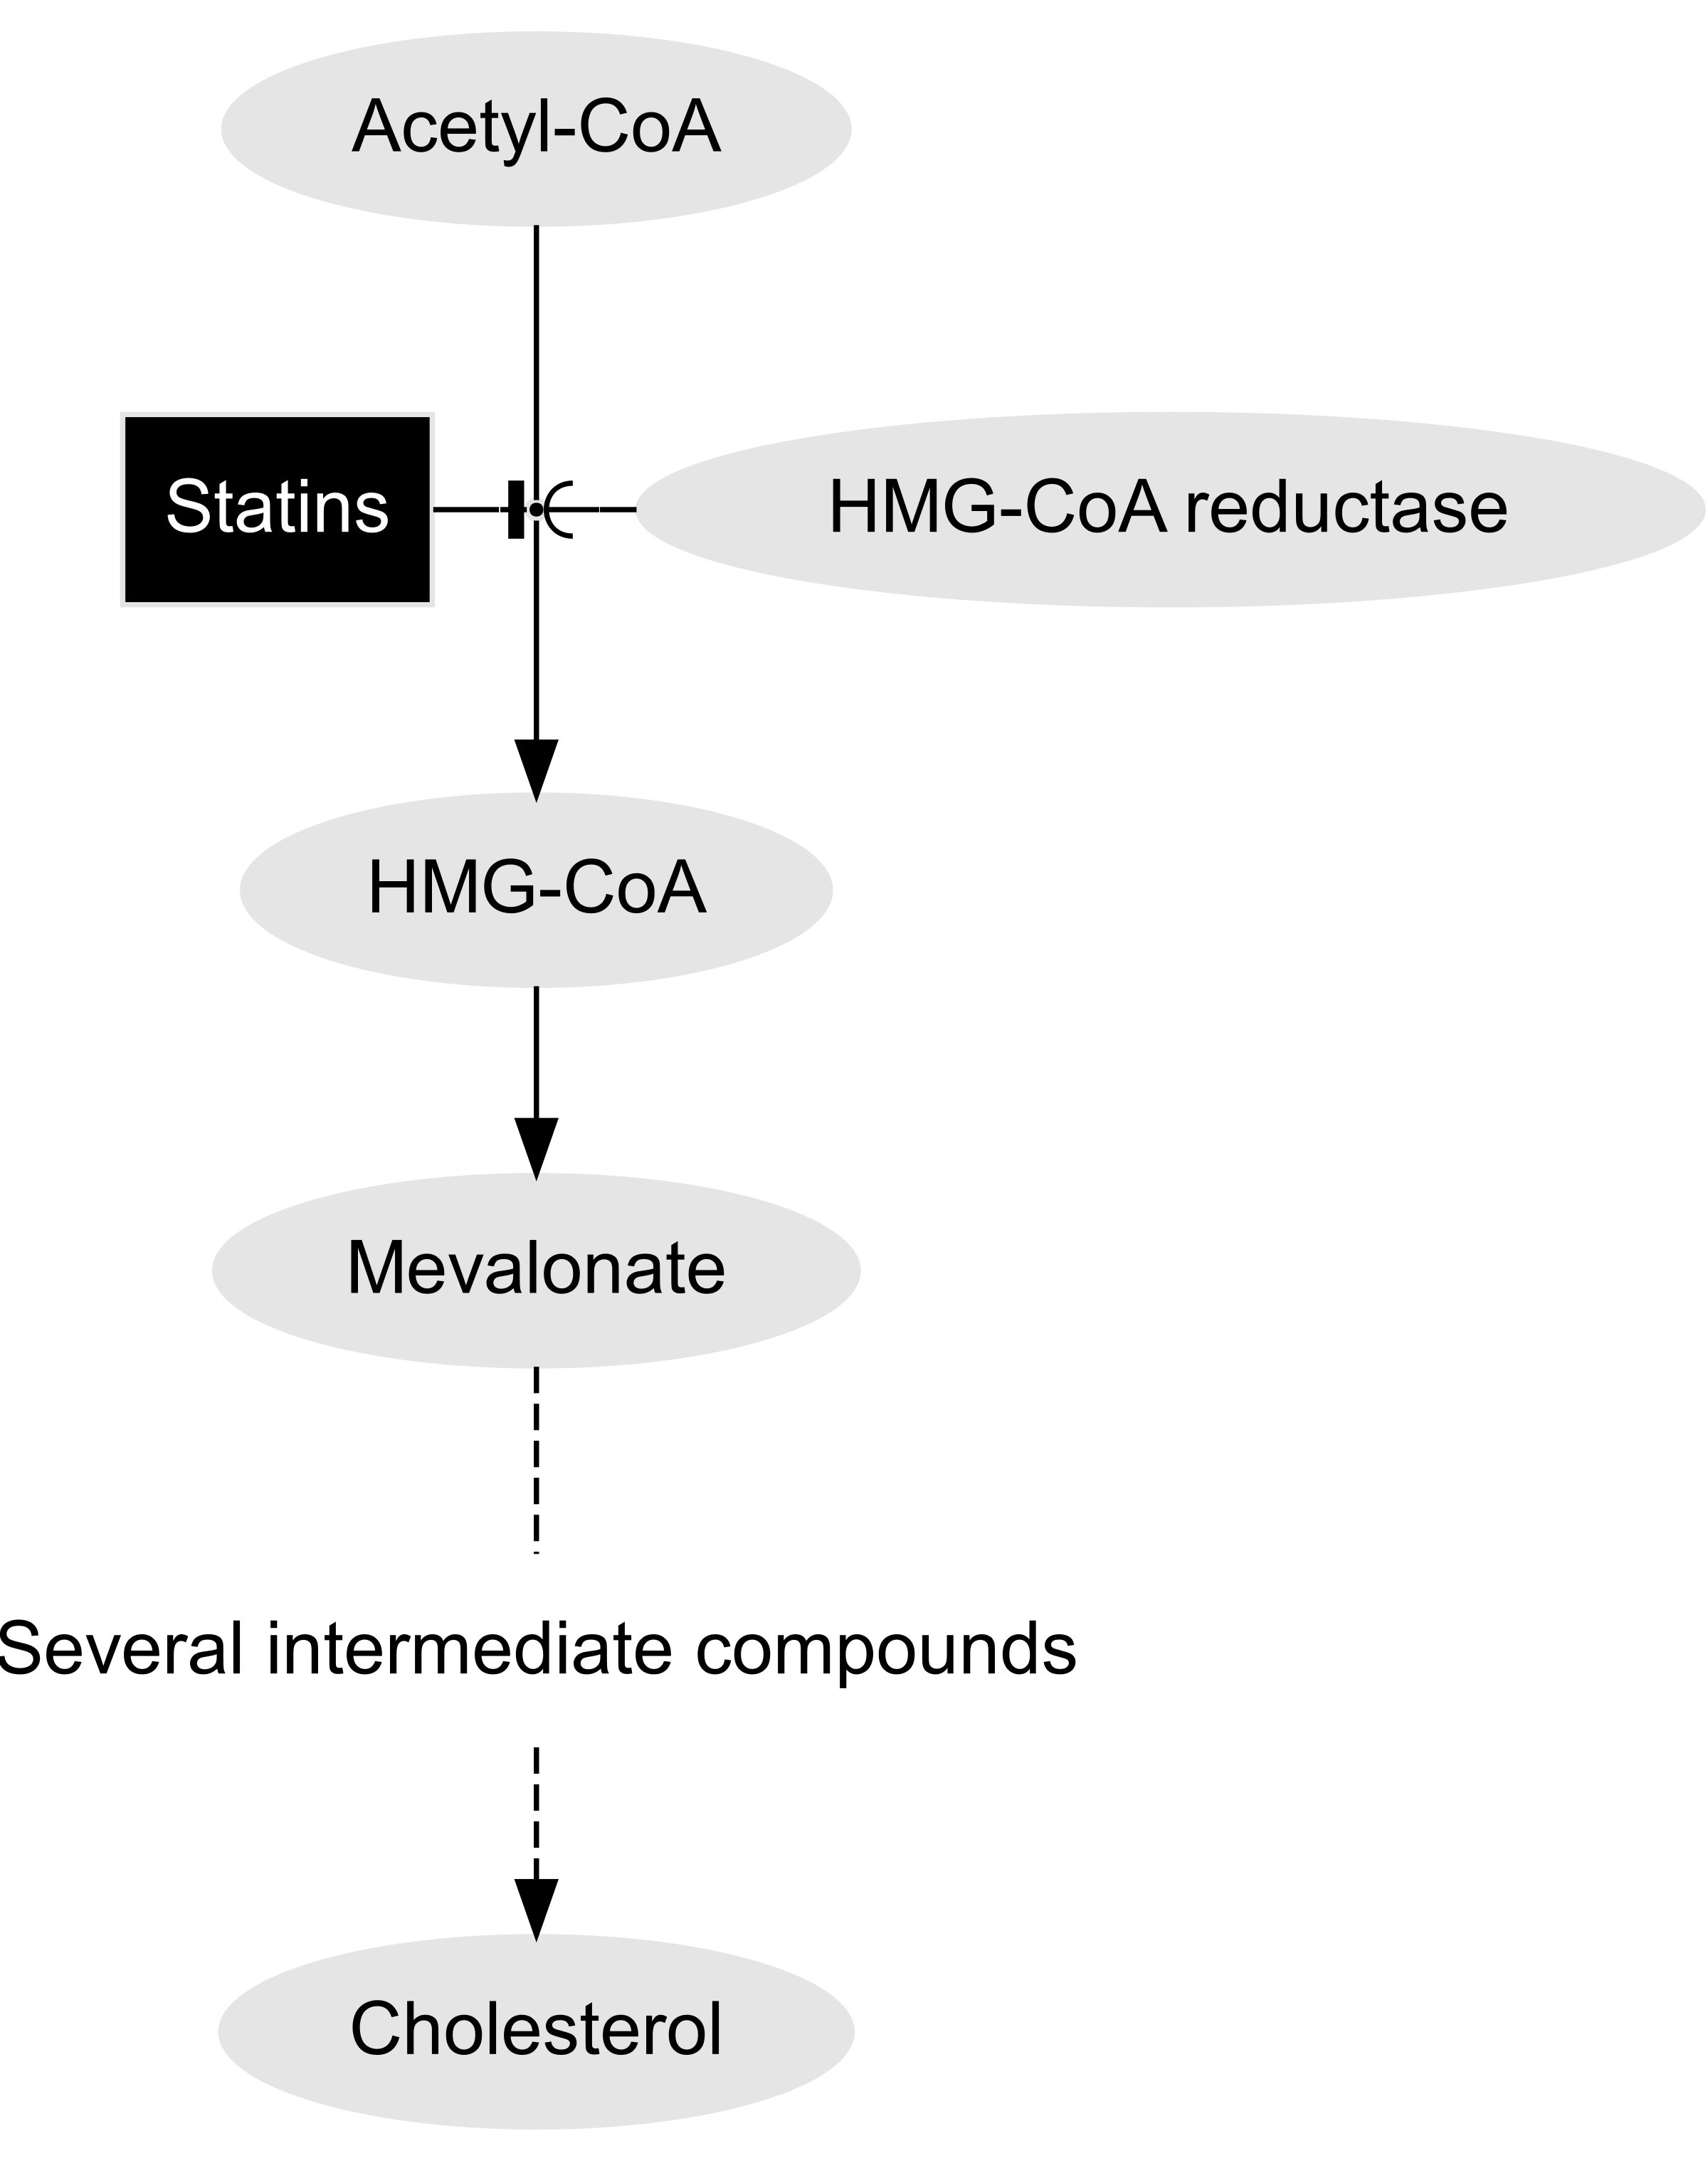
\includegraphics[width=0.5\linewidth]{figures/background/statinPath} 

}

\caption[Statin mechanism of action]{Overivew of statins mechanism of action, inhibiting HMG-CoA reductase which controls the conversion of HMG-CoA to mevalonate, the rate-limiting step in cholesterol biosynthesis.}\label{fig:statin-mechanisam}
\end{figure}

~

Several statin treatments have been widely available for some time (see Table \ref{tab:statinOverview-table}). Depending on the statin and dosage prescribed, the average reduction in LDL-c concentrations ranges from 15\% with low-intensity regimen (e.g.~ravastatin 5 mg/day) up to 60\% with a high-intensity regimen (e.g.~rosuvastatin 80 mg/day).\textsuperscript{\protect\hyperlink{ref-collins2016a}{30},\protect\hyperlink{ref-law2003}{31}} Statins also vary with regard to their lipophilicity (the extent to which they are lipid soluble), affecting their localisation within the body, with hydophilic statins being concentrated in the liver and lipophilic statins circulating more widely.\textsuperscript{\protect\hyperlink{ref-schachter2005}{32}} This may create a divide in the pleiotropic affects of statins with differing lipophilicity, particularly given the ability of lipophilic statins to permeate the blood brain barrier.\textsuperscript{\protect\hyperlink{ref-sierra2011}{33}}

~





\begin{table}[H]

\caption[Overview of common statins]{\label{tab:statinOverview-table}Overview of commonly-prescribed statins, summarising their approval date (US), properties and lipid-lowering effect.}
\centering
\begin{tabular}[t]{>{\centering\arraybackslash}p{6em}>{\centering\arraybackslash}p{6em}>{\centering\arraybackslash}p{6em}>{\centering\arraybackslash}p{6em}>{\centering\arraybackslash}p{7.6em}}
\toprule
\textbf{Name} & \textbf{Brand name} & \textbf{Year approved} & \textbf{Properties} & \textbf{Lipid-lowering effect}\\
\midrule
\textbf{Atorvastatin} & Lipitor & 1996 & Lipophilic & +++\\
\midrule
\textbf{Pravastatin} & Lipostat & 1989 & Hydrophilic & +\\
\midrule
\textbf{Rosuvastatin} & Crestor & 2003 & Hydrophilic & ++++\\
\midrule
\textbf{Simvastatin} & Zocor & 1992 & Lipophilic & ++\\
\bottomrule
\end{tabular}
\end{table}

~

\hypertarget{other-lipid-regulating-agents-lra}{%
\subsection{Other lipid regulating agents (LRA)}\label{other-lipid-regulating-agents-lra}}

There are several other interventions that can be used to modify a persons lipid profile, which each acting in slightly different ways (Table \ref{tab}). However, in general, these treatments are either used as adjunct (additional) treatments with statins therapy or are used in situations where statins are contra-indicated or not tolerated.

The most commonly used non-statin therapeutic is ezetimibe,\textsuperscript{\protect\hyperlink{ref-kosoglou2005}{34}} which prevents intestinal absorption of cholesterol. However, when used alone, it has a limited LDL-c lowering effect, leading to the creation of combined statin/ezetimibe therapies (both compounds contained in a single pill, as opposed to complimentary treatments).\textsuperscript{\protect\hyperlink{ref-genest2006}{35}}

Fibrates provide a second example of non-statin therapy. They are used to treat hypertriglyceridaemia by reducing production of triglyceride carrying compounds in the liver. They are commonly used in patients with mixed hyperlipidaemia if treatment with statins has failed to sufficiently control cholesterol levels.

Finally, PCSK9 inhibitors (or PCSK9i) are a relatively new treatment with strong lipid lowering effects, lauded as a potential alternative to statins.\textsuperscript{\protect\hyperlink{ref-chaudhary2017}{36}} Their mechanism of action is to bind to and inhibit PCSK9, which breaks down LDL-c receptors on the surface of the liver, thus allowing more LDL-c to be internalised and broken down.

Other therapies targeting triglycerides exist, including nicotinic acids\textsuperscript{\protect\hyperlink{ref-mckenney2004new}{37}} and omega-3-fatty acids,\textsuperscript{\protect\hyperlink{ref-skulas-rayannc.2019}{38}} but they far less effective in LDL-c lowering than the therapies described above.

~



\begin{table}[H]

\caption{\label{tab:lipidTreatments-table}Summary of available treatments for hyperlipidaemia.}
\centering
\begin{tabular}[t]{>{\raggedright\arraybackslash}p{8em}>{\raggedright\arraybackslash}p{8em}>{\raggedright\arraybackslash}p{8em}>{\raggedright\arraybackslash}p{8em}}
\toprule
\textbf{Treatment} & \textbf{Effect} & \textbf{Mechanism of action} & \textbf{Examples}\\
\midrule
\textbf{HMG CoA reductase inhibitors (statins)} & Lowers LDL-c \& TG \newline Raises HDL-c & Inhibits cholesterol biosynthesis pathway in the liver & Atorvastatin, \newline Simvastatin, \newline Pravastatin\\
\midrule
\textbf{Ezetimibe} & Lowers LDL-c & Prevents absorption of cholesterol from diet & \\
\midrule
\textbf{Bile acide sequestrants} & Lowers LDL-c & Prevent bile acid reabsorption in the gastro-intestinal tract, increasing conversion of cholesterol to bile acids & Colestipol\\
\midrule
\textbf{Proprotein convertase subtilisin kexin 9 (PCSK9) inhibitors} & Lowers LDL-c & Bind to PSCK9 protein, preventing it from breaking down LDL receptors on heptatic cells, increasing cholesterol uptake & Evolocumab, \newline Alirocumab\\
\bottomrule
\end{tabular}
\end{table}

~

\hypertarget{evidence-association}{%
\section{Evidence for the association between blood lipids and dementia}\label{evidence-association}}

This section provides an overview of the varying sources of evidence on the relationship between blood lipid levels and dementia risk.

\hypertarget{intro-basic-science}{%
\subsection{Basic science}\label{intro-basic-science}}

A role for lipids in the aetiology of the dementia is supported by both genetic linkage studies and functional cell biology studies. The generation of the amyloid plaques found in the brains of Alzheimer's patients is cholesterol dependent,,\textsuperscript{\protect\hyperlink{ref-burns2003}{39},\protect\hyperlink{ref-mizuno1999}{40}} while the most established genetic risk factor for late-onset dementia, apolipoprotein E (ApoE), is involved in cerebral cholesterol transport. Several other genes involved in cholesterol transport have also been found to be associated with increased AD susceptibility.\textsuperscript{\protect\hyperlink{ref-beecham2014}{41}--\protect\hyperlink{ref-meng2007}{43}}

Despite these results, evidence from the diverse range of epidemiological studies on this topic has been inconclusive.

\hypertarget{observational-studies}{%
\subsection{Observational studies}\label{observational-studies}}

By far the largest source of evidence on the relationship between comes from observational designs. Several studies have examined the relationships between concentrations of serum lipids (total cholesterol (TC), low density lipoprotein cholesterol (LDL-c), high density lipoprotein cholesterol (HDL-c) and triglycerides) and both Alzheimer's disease and vascular dementia and reported extremely varied results. In some studies, a high serum cholesterol concentration has been found to be associated with an increase in susceptibility to AD,\textsuperscript{\protect\hyperlink{ref-kivipelto2002}{44}--\protect\hyperlink{ref-whitmer2005}{48}} however others have shown no association,\textsuperscript{\protect\hyperlink{ref-li2005a}{49}--\protect\hyperlink{ref-tan2003a}{52}} or a reduced susceptibility.\textsuperscript{\protect\hyperlink{ref-mielke2005}{53},\protect\hyperlink{ref-reitz2004a}{54}} With regards vascular dementia, decreased levels of HDL-c appear to be associated with increased risk,\textsuperscript{\protect\hyperlink{ref-reitz2004a}{54}} while for LDL-c, studies have reported both positive and negative associations.\textsuperscript{\protect\hyperlink{ref-reitz2004a}{54},\protect\hyperlink{ref-moroney1999}{55}}

Several previous systematic review of observational studies examining the effect of lipids\textsuperscript{\protect\hyperlink{ref-anstey2015}{56}} and lipid-regulating agents\textsuperscript{\protect\hyperlink{ref-chu2018}{57},\protect\hyperlink{ref-poly2020c}{\textbf{poly2020c?}}} on dementia outcomes have been performed. However, these reviews have several limitations. Many did not consider grey literature sources (see Section \ref{diverse-sources-preprints}). Additionally, many of the reviews of observational studies did not perform any risk-of-bias assessment\textsuperscript{\protect\hyperlink{ref-chu2018b}{\textbf{chu2018b?}}} or used an outdated assessment tool.\textsuperscript{\protect\hyperlink{ref-anstey2015}{56},\protect\hyperlink{ref-poly2020c}{\textbf{poly2020c?}}}

\hypertarget{randomised-controlled-trials}{%
\subsection{Randomised controlled trials}\label{randomised-controlled-trials}}

In terms of the central research of this thesis, RCTs of statin therapy can be used to provide indirect evidence for the effect of reducing blood LDL-c levels on dementia risk.

However, RCTs may be infeasible if the outcome of interest is one with a long prodomal period, such as dementia (see Section \ref{underlying-pathologies}), as they would require extremely long and costly follow-up.\textsuperscript{\protect\hyperlink{ref-ritchie2015}{58}} It is no surprise then that the two previous trials providing evidence on the effect of statins on dementia risk, identified by a recent Cochrane review,\textsuperscript{\protect\hyperlink{ref-mcguinness2016a}{\textbf{mcguinness2016a?}}} are in fact trials of statins for the prevention of coronary related outcomes.

While being widely cited, these studies have major limitations that reduce their utility as a source of evidence on the effect of statin treatment on in assessing the impact of lipid-lowering treatment on dementia risk. Firstly, there was no clinical cognitive evaluation of patients to determine a dementia outcome. One of the trials, the Prospective Study of Pravastatin in the Elderly (PROSPER) trial,\textsuperscript{\protect\hyperlink{ref-trompet2010}{59}} reported not on dementia outcomes but on the change in cognitive scores over a mean of 3.2 years. As highlighted in Section \ref{diagnostic-criteria}, a ``change in score'' alone is insufficient to diagnose a dementia outcome. The second trial, the Medical Research Council/British Health Foundation Protection Study,\textsuperscript{\protect\hyperlink{ref-2002}{\textbf{2002?}}} found no effect of simvastatin on dementia (OR: 1.00, 95\%CI: 0.61-1.65), but did not report how the outcome was assessed/recorded within the trial.

Additionally, the two trials did not make any effort to assign an underlying pathology to each case, instead reporting an all-cause dementia outcome. As discussed in Section \ref{underlying-pathologies}, the different underlying pathology of dementia have different mechanisms of action, and so it is not gauranteed that the effect of statins would be consistent across them.

Both trials were also limited by the relatively short follow-up period examined, expected when the primary outcome of the trials were coronary related conditions rather than dementia.\textsuperscript{\protect\hyperlink{ref-trompet2010}{59},\protect\hyperlink{ref-2002}{\textbf{2002?}}} The PROSPER trial had a mean follow-up of 3.2 years, while the MRC/BHF Protection Study estimated risk at 5 years of follow-up. Given the long lag time between non-symptomatic onset of dementia and clinical presentation, it is likely that these durations are insufficient to fully capture the onset of dementia. Finally, as they included only patients at high vascular risk, their generalisability to other settings is limited.\textsuperscript{\protect\hyperlink{ref-mcguinness2016b}{\textbf{mcguinness2016b?}}}

\hypertarget{mendelian-randomisation}{%
\subsection{Mendelian randomisation}\label{mendelian-randomisation}}

Newer methodological approaches, such as Mendelian randomisation (MR),\textsuperscript{\protect\hyperlink{ref-daveysmith2014}{60}} have also been used to examine the effect of varying lipid levels on dementia risk in an effort to combat the risk of reverse causation and residual confounding inherent to observational studies.\textsuperscript{\protect\hyperlink{ref-greenland2000}{61}} In brief, MR uses genetic variants that are both strongly associated with the exposure of interest and are independent from potential confounders to strengthen causal inference.\textsuperscript{\protect\hyperlink{ref-daveysmith2014}{60}} The analytic method relies on several assumptions about the instrumental variable (IV),\textsuperscript{\protect\hyperlink{ref-davies2018}{62}} namely that:

\begin{enumerate}
\def\labelenumi{\arabic{enumi}.}
\tightlist
\item
  the IV is associated with the exposure of interest (the relevance assumption);
\item
  the IV and outcome do not share a common cause (the independence assumption); and
\item
  the IV does not affect the outcome other than via the exposure (the exclusion restriction assumption).
\end{enumerate}

Recent MR studies indicated that genetically determined low levels of LDL-c may cause a reduction in AD risk.\textsuperscript{\protect\hyperlink{ref-larsson2017c}{63},\protect\hyperlink{ref-ostergaard2015}{64}} However, the effect was attenuated in sensitivity analysis that exclude the region surrounding the ApoE gene, the strongest known risk factor for Alzheimer's disease.\textsuperscript{\protect\hyperlink{ref-kim2009}{65}} Inclusion of ApoE4 variants invalidates the exclusion restriction criteria (Assumption 3, above), as the risk reduction observed may be driven by variants in this region via a pathway independent of lipid levels. This was supported by further MR studies where \emph{ApoE4} variants were intentionally excluded.\textsuperscript{\protect\hyperlink{ref-benn2017}{66}}

Despite the increasing number of MR studies examining this topic, no systematic review of this study design as a source of evidence has been performed.

~

In summary, multiple sources of evidence exist on the relationship between statins and dementia. In the next section, I introduce the synthesis of diverse sources of evidence as the theoretical framework used in this thesis.

\hypertarget{theoretical-framework-evidence-synthesis}{%
\section{Theoretical framework: Evidence synthesis}\label{theoretical-framework-evidence-synthesis}}

Evidence synthesis is the process of finding and integrating information from several sources to examine a research question.\textsuperscript{\protect\hyperlink{ref-donnelly2018a}{67}} A common tyoe of evidence synthesis is a systematic review, either with or without a meta-analysis.\textsuperscript{\protect\hyperlink{ref-chandler2019chapter}{68}}

The results of an evidence synthesis exercise can be used to provide a more definitive answer to that question or, failing that, to highlight gaps in the existing evidence base. The ability to identify these gaps is particularly useful in guiding future research to address questions that have yet to be answered.

This thesis seeks to use an evidence synthesis framework to assess the effect of lipids, and treatments that influence lipid levels, on dementia outcomes.
Specifically, this thesis considers three concepts within the umbrella term of evidence synthesis:

\begin{itemize}
\tightlist
\item
  Inclusion of preprints
\item
  Triangulation across evidence sources
\item
  Individual patient data meta-analysis
\end{itemize}

These three elements are expanded on below and are used to frame the research presented in the subsequent Chapters.

\hypertarget{diverse-sources-preprints}{%
\subsection{Inclusion of preprints}\label{diverse-sources-preprints}}

The importance of including grey (or gray) literature in systematic reviews is widely acknowledged. Meta-research studies have demonstrated that systematic reviews excluding grey literature sources overestimate the effect of interventions.\textsuperscript{\protect\hyperlink{ref-conn2003}{69}--\protect\hyperlink{ref-hopewell2007}{71}} Common, well-accepted forms of grey literature include conference abstracts and theses.\textsuperscript{\protect\hyperlink{ref-lefebvre2019searching}{72}}

A important developing source of grey literature are preprints. Defined by the Committee on Publication Ethics (COPE) as `scholarly manuscript{[}s{]} posted by the author(s) in an openly accessible platform, usually before or in parallel with the peer review process'\textsuperscript{\protect\hyperlink{ref-committeeonpublicationethicscope2018}{73}}, preprints serve several purposes. They are used to establish primacy when submitting to a journal where the peer-review process may take several months,\textsuperscript{\protect\hyperlink{ref-vale2016}{74}} to rapidly disseminate research findings, as occurred during the COVID-19 pandemic,\textsuperscript{\protect\hyperlink{ref-fraser2020preprinting}{75}} and to make available publications that may not have been accepted elsewhere in an attempt to combat publication bias or the ``file-drawer'' effect.\textsuperscript{\protect\hyperlink{ref-rosenthal1979}{76}}

One of the major criticisms of using preprints as an evidence source is that they have not yet undergone formal peer review.\textsuperscript{\protect\hyperlink{ref-maslove2018}{77},\protect\hyperlink{ref-schalkwyk2020}{78}} However, this approach assigns substantial weight to peer-review as a indicator of ``quality'', and is at odds with the acceptance of non-reviewed conference proceedings as an evidence source.\textsuperscript{\protect\hyperlink{ref-lefebvre2019searching}{72},\protect\hyperlink{ref-mahood2014}{79}} The argument for including preprints as an evidence source is further strengthened by results that demonstrate preprinted studies seldom change following peer review. Meta-studies of the concordance between preprinted and published studies showed that results were broadly comparable between the two, indicating that while the numerical results may change, the overall interpretation of the results were consistent in the majority of cases.\textsuperscript{\protect\hyperlink{ref-klein2019}{80},\protect\hyperlink{ref-nicholson2021}{81},\protect\hyperlink{ref-shi2021a}{\textbf{shi2021a?}}} This indicates that preprints should be considered a reliable reflection of a given study.

In this thesis, preprints are considered an important source of evidence, in contrast to previous reviews on this topic. However, as with many sources of grey literature,\textsuperscript{\protect\hyperlink{ref-mahood2014}{79}} there are several logistical issues with carrying out systematic searches in preprint repositories. As such, to enable the inclusion of preprints in the systematic review described in Chapters \ref{sys-rev-methods-heading}, a new tool addressing these issues is presented in Chapter \ref{sys-rev-tools}.

\hypertarget{intro-triangulation}{%
\subsection{Triangulating across study designs}\label{intro-triangulation}}

As illustrated in Section \ref{evidence-association}, several diverse epidemiological methods have been used to examine the effect of varying blood lipid levels on dementia risk. However, each method is limited by its own biases. Aetiological triangulation is a developing evidence synthesis method that seeks to exploit these inherent differences in study design, and as a result, in biases.\textsuperscript{\protect\hyperlink{ref-lawlor2016a}{\textbf{lawlor2016a?}}} If several sources of evidence are available and point towards identical conclusions about an exposure-outcome relationship, and these sources are at risk of unrelated biases, this strengthens our confidence in the result. The ideal scenario is where predicted sources of bias are likely to be in competing directions, strengthen the effect of the exposure and the other to attenuate it.\textsuperscript{\protect\hyperlink{ref-lawlor2016a}{\textbf{lawlor2016a?}}} As such, triangulating these results can provides us a middle-ground between the competing directions of bias. A triangulation approach can also prove useful in a prospective manner, helping to design new studies that are at risk of different sources of bias to that already available from the published literature.\textsuperscript{\protect\hyperlink{ref-munafo2018}{82}}

This thesis seeks to apply a triangulation approach to provide the best available evidence on the effect of lipids, and lipid regulating agents, on dementia outcomes.

All existing evidence, regardless of study design, is first identified by the by the systematic review presented inChapters \ref{sys-rev-methods-heading}/\ref{sys-rev-results-heading}. Risk-of-bias assessment using a domain-based tool is already a recommended part of the systematic review process, but is particularly important to a triangulation exercise.\textsuperscript{\protect\hyperlink{ref-page2021}{83},\protect\hyperlink{ref-mcguinness2018}{84},\protect\hyperlink{ref-sterne2019a}{\textbf{sterne2019a?}}} As such, a core component of the review is a comprehensive domain-based risk-of-bias assessment for all included studies.

Finally all evidence, both pre-existing and produced as part of this thesis (Chapter \ref{cprd-analysis-heading} and \ref{ipd-analysis-heading}), are triangulated in Chapter \ref{dicussion-heading}.

\hypertarget{individual-patient-data-meta-analysis}{%
\subsection{Individual patient data meta-analysis}\label{individual-patient-data-meta-analysis}}

Individual patient data meta-analyses are commonly held to represent the gold standard in evidence synthesis methodology.\textsuperscript{\protect\hyperlink{ref-riley2010}{85},\protect\hyperlink{ref-stewart1993}{86}} IPD methods seek to obtain the raw data from each study identified in a systematic review, rather than basing the meta-analysis on summary results extracted from the literature.\textsuperscript{\protect\hyperlink{ref-riley2010}{85}}

In the context of this thesis, if lipids are found to have a causal role in development of dementia, evidence-based preventative strategies would be best informed by identifying the types of individuals who are most likely to receive benefit from treatment with lipid-modifying agents.\textsuperscript{\protect\hyperlink{ref-arain2009}{87}--\protect\hyperlink{ref-mccartney2016}{89}} However, if primary studies do not present results stratified by covariates of interest, meta-analyses of summary-level data on this topic often have limited ability to examine research questions related to exposure-covariate interactions.\textsuperscript{\protect\hyperlink{ref-riley2010}{85}} In terms of this thesis, patient sex is considered to be of particular interest.\textsuperscript{\protect\hyperlink{ref-arain2009}{87},\protect\hyperlink{ref-letenneur1999}{90}}

An IPD meta-analysis of lipid levels on dementia outcomes would overcome this limitation of summary-level data, as access to the raw data allows for an analysis that investigates these interactions.\textsuperscript{\protect\hyperlink{ref-riley2020}{91}} This approach has the added benefit of allowing a common set of inclusion criteria and statistical model to be applied across all datasets, potentially eliminating some important sources of heterogeneity.\textsuperscript{\protect\hyperlink{ref-stewart2002}{92}}

Despite their advantages, IPD meta-analysis are rarely performed.\textsuperscript{\protect\hyperlink{ref-tugwell2010}{93}} Factors limiting their uptake include the increased time and effort they require when compared to a summary-level analysis, and the low success rate associated with obtaining the raw data.\textsuperscript{\protect\hyperlink{ref-nevitt2017a}{94},\protect\hyperlink{ref-ventresca2020}{95}} The data underlying primary studies are frequently not publicly available,\textsuperscript{\protect\hyperlink{ref-alsheikh-ali2011}{96},\protect\hyperlink{ref-federer2018a}{\textbf{federer2018a?}}} and the availability of data ``available on request from authors'' declines rapidly over time.\textsuperscript{\protect\hyperlink{ref-vines2014}{97}} Several systematic barriers to open data sharing have been identified\textsuperscript{\protect\hyperlink{ref-vanpanhuis2014a}{\textbf{vanpanhuis2014a?}}}. Of particular concern for biomedical IPD analyses are legal issues surrounding the sharing of medical data, motivated by concerns around patient privacy.\textsuperscript{\protect\hyperlink{ref-wartenberg2010}{98}}

In response to these limitations, new collaborative initiatives have developed to enable rapid access to relevant data in a secure supported workshop. The most import in relation to this thesis is the Dementia Platform UK (DPUK),\textsuperscript{\protect\hyperlink{ref-bauermeister2020}{99}} which aims to provide access to several dementia-related datasets via a single simplified application process.

I will will attempt to obtain the raw data from relevant primary studies identified by the systematic review in Chapters \ref{sys-rev-methods-heading}/\ref{sys-rev-results-heading}. Any data obtained will be combined with that available from the DPUK portal as part of an individual participant data meta-analysis in Chapter \ref{ipd-analysis-heading}, enabling the assessment of the effect of lipids on dementia stratified by key variables such as sex.

\hypertarget{background-thesis-overview}{%
\section{Thesis overview}\label{background-thesis-overview}}

\hypertarget{aims-and-objectives}{%
\subsection{Aims and objectives}\label{aims-and-objectives}}

The over-arching aim of this thesis is to explore the relationship between blood lipid levels, and by extension treatments that modify blood lipid levels such as statins, and the subsequent risk of dementia and related outcomes

The specific research objectives that this thesis seeks to address are:

\begin{itemize}
\tightlist
\item
  To create a tool that allows for the inclusion of health related preprints in evidence syntheses in a systematic and reproducible manner
\item
  To review all available evidence across multiple diverse study designs to assess the effect of lipids and lipid regulating agents on dementia risk
\item
  To examine whether there is evidence for an effect of lipid-regulating agents on dementia and related outcomes in a large scale population-based cohort, the Clinical Practice Research Datalink (CPRD)
\item
  To meta-analyse raw dementia-related datasets as part of a individual participant data (IPD meta-analysis) to produce evidence on exposure-covariate interactions
\end{itemize}

\hypertarget{thesis-structure}{%
\subsection{Structure}\label{thesis-structure}}

Chapters are self-contained, presenting the methods and results of that specific research project. They are bookended by introductory and discussion sections which place the methods and results in context. Each chapter is prefaced by a ``Lay'' or plain English summary, developed with input from the Patient and Public Advisory Group (see Section \ref{disc-PPI} for a discussion of the group's involvement and Appendix \ref{appendix-ppi} for more detail on the group).

\begin{itemize}
\tightlist
\item
  \textbf{Chapter \ref{background-heading}:} Background information on dementia and blood lipid levels. This chapter provides an introduction to the topics covered in this thesis to non-subject area experts, and discusses the motivation for the remainder of the thesis.
\item
  \textbf{Chapter \ref{sys-rev-tools-heading}:} This Chapter introduces a new tool, \texttt{medrxivr}, which was used to developed to allow for systematic searches of the health-related preprint repositories.
\item
  \textbf{Chapters \ref{sys-rev-methods-heading}/\ref{sys-rev-results-heading}:} These Chapters describe, respectively, the methods and results of a comprehensive systematic review and meta-analysis. This review examined all available evidence on the effect of blood lipids, and interventions that modified blood lipids, on dementia outcomes.
\item
  \textbf{Chapter \ref{cprd-analysis-heading}:} This Chapter examines the relationship between lipid-regulating agent use and dementia outcomes in the Clinical Practice Research Datalink, a large primary care electronic health record database.
\item
  \textbf{Chapter \ref{ipd-heading}:} This Chapter describes an individual patient data analysis of several longitudinal cohort studies to describe the relationship between blood serum lipids and dementia outcomes, stratified by important covariates such as sex.
\item
  \textbf{Chapter \ref{discussion-heading}}: This Chapter integrates the diverse evidence identified by, and produced as part of, this thesis. The overall strengths and weaknesses of this project are discussed in detail, and further avenues of research are suggested.
\end{itemize}

\hypertarget{thesis-output}{%
\section{Outputs from this thesis}\label{thesis-output}}

The outputs of this thesis are detailed below, and include peer-reviewed papers, presentations, and open-source evidence synthesis tools.

\hypertarget{contributions-to-the-scientific-literature}{%
\subsection{Contributions to the scientific literature}\label{contributions-to-the-scientific-literature}}

During the course of this thesis, I have made several contributions to the scientific literature. Those arising from or directly related to the contents of this submission are presented below.

~

\emph{\textbf{McGuinness, L. A.}, and L Schmidt. (2020) medrxivr: Accessing and searching medRxiv and bioRxiv preprint data in R. Journal of Open Source Software 5.54 2651. DOI: \href{https://doi.org/10.21105/joss.02651}{10.21105/joss.02651}}

A paper introducing the open-source preprint search tool described in Chapter \ref{sys-rev-tools-heading}. As is common for journal articles describing software, the paper is intentionally short providing only a broad overview of the tool while extensive documentation is available from the project website (see Section \ref{sys-rev-tools-intro} for more details).

~

\emph{Hennessy, E. A., Acabchuk, R., Arnold, P. A., Dunn, A. G., Foo, Y. Z., Johnson, B. T., Geange, S. R., Haddaway, N. R., Nakagawa, S., Mapanga, W., Mengersen, K., Page, M., Sánchez-Tójar, A. Welch, V., \textbf{McGuinness L. A.} (2021). Ensuring Prevention Science Research is Synthesis-Ready for Immediate and Lasting Scientific Impact. Prevention Science . DOI: \href{https://doi.org/10.1007/s11121-021-01279-8}{10.1007/s11121-021-01279-8}}

The experience of extracting data for the systematic review in Chapters \ref{sys-rev-methods-heading}/\ref{sys-rev-results-heading} inspired a practical guide for researchers. This piece was co-written with Dr.~Emily Hennessy (see Author Declarations in the front materials).

~

\emph{\textbf{McGuinness, L. A.}, and Higgins J. P. T. (2020) ``Risk‐of‐bias VISualization (robvis): An R package and Shiny web app for visualizing risk‐of‐bias assessments.'' Research Synthesis Method). DOI: \href{https://doi.org/10.1002/jrsm.1411}{10.1002/jrsm.1411}}

The tool used to visualise the risk-of-bias assessments in Chapters \ref{sys-rev-methods-heading}/\ref{sys-rev-results-heading} has been published in Research Synthesis Methods. See Appendix \ref{appendix-robvis} for more details on this tool. Note that this publication does not describe the recently-developed functionality for producing bias direction plots, as described in Chapter \ref{tri-heading}.

~

\emph{\textbf{McGuinness, L. A.}, and Sheppard A. L. 2020. ``A Descriptive Analysis of the Data Availability Statements Accompanying Medrxiv Preprints and a Comparison with Their Published Counterparts.'' PLOS ONE 16(5): e0250887. DOI: \href{https://doi.org/10.1371/journal.pone.0250887}{10.1371/journal.pone.0250887}}

Using the tool described in Chapter \ref{sys-rev-tools}, I lead a ``research-on-research'' study to assess the concordance between the openness of data availability statements accompanying a sample of medRxiv preprints and their published counterparts.

~

For information on additional contributions to the scientific literature not directly related to this thesis, see Appendix \ref{appendix-publications}.

~

\hypertarget{presentationstalks}{%
\subsection{Presentations/Talks}\label{presentationstalks}}

\emph{``Identifying and triangulating all available evidence on the effect of blood lipids and statins on dementia outcomes''}: Poster presentation, Alzheimer's Association International Conference 2021.
~

\emph{``medrxivr: A new tool for searching for and retrieving records and PDFs from the medRxiv preprint repository''}: Accepted oral presentation abstract, Cochrane Colloquium 2020 (note: event was cancelled due to the COVID-19 pandemic)

~

\emph{``On the shoulders of giants'': advantages and challenges to building on established evidence synthesis packages, using the \{robvis\} package as a case study"}: Oral presentation, Evidence Synthesis and Meta-Analysis in R Conference (ESMARConf) 2021.

~

\emph{``RoB 2.0: A revised tool to assess risk of bias in randomized trials''}: Webinar, co-presented with Dr.~Theresa Moore as part of the Evidence Synthesis Ireland Methods Series.

\hypertarget{outputs-software}{%
\subsection{Software}\label{outputs-software}}

\textbf{\texttt{medrxvir}}

An R package that allows users to easily search and retrieve bibliographic data from the medRxiv\textsuperscript{\protect\hyperlink{ref-rawlinson2019}{100}} and bioRxiv\textsuperscript{\protect\hyperlink{ref-sever2019}{101}} preprint repositories. See Chapter \ref{sys-rev-tools-heading} for more details. Install a stable version of the package from the Comprehensive R Archive Network (CRAN), or alternatively install the development version from GitHub, using:

\begin{Shaded}
\begin{Highlighting}[]
\CommentTok{\# CRAN version}
\FunctionTok{install.packages}\NormalTok{(}\StringTok{"medrxivr"}\NormalTok{)}

\CommentTok{\# Development version}
\NormalTok{devtools}\SpecialCharTok{::}\FunctionTok{install\_github}\NormalTok{(}\StringTok{"ropensci/medrxivr"}\NormalTok{)}
\end{Highlighting}
\end{Shaded}

~

\textbf{\texttt{robvis}}

An R package and associated \texttt{shiny} web application that allows users to easily visualize the results of the risk-of-bias assessments performed as part of a systematic review. See Appendix \ref{appendix-robvis} for more details. Install a stable version of the package from CRAN, or alternatively install the development version from GitHub, using:

\begin{Shaded}
\begin{Highlighting}[]
\CommentTok{\# CRAN version}
\FunctionTok{install.packages}\NormalTok{(}\StringTok{"robvis"}\NormalTok{)}

\CommentTok{\# Development version}
\NormalTok{devtools}\SpecialCharTok{::}\FunctionTok{install\_github}\NormalTok{(}\StringTok{"mcguinlu/robvis"}\NormalTok{)}
\end{Highlighting}
\end{Shaded}

~

\hypertarget{summary}{%
\section{Summary}\label{summary}}

This Chapter has provided background information on the core elements of the central research question, framed the research presented in this thesis in the context of an evidence synthesis framework, and described the contributions of this thesis to the scientific literature.

\newpage

\hypertarget{references}{%
\section{References}\label{references}}

\begin{savequote}
Why are open source statistical programming\\
languages the best?

Because they R.
\qauthor{--- Bealy, 2013\textsuperscript{\protect\hyperlink{ref-bealy2013}{102}}}\end{savequote}



\hypertarget{sys-rev-tools-heading}{%
\chapter{medrxivr: an R package for systematically searching biomedical preprints}\label{sys-rev-tools-heading}}

\minitoc 

\hypertarget{lay-summary-1}{%
\section{Lay summary}\label{lay-summary-1}}

Preprints are copies of academic manuscripts that are posted online in advance of being formally published by an academic journal. They represent an important source of scientific literature. A new software program called \texttt{medrxivr} was created to allow researchers to find preprints related to their research in a transparent and reproducible way. Development of this tool was an essential part of this thesis, as preprints represent a key source of information needed for the research reported in future chapters.

\hypertarget{sys-rev-tools-intro}{%
\section{Introduction}\label{sys-rev-tools-intro}}

Preprints represent an increasingly important source of scientific information (see Section \ref{diverse-sources-preprints}). As a result, repositories of preprinted articles should be considered a distinct but complementary information source when reviewing the evidence base as part of a systematic review. The two key repositories in the health science are bioRxiv, established in 2013,\textsuperscript{\protect\hyperlink{ref-sever2019}{101}} and medRxiv, which launched in 2019 and was designed to replace the ``Epidemiology'' and ``Clinical Trial'' categories of bioRxiv.\textsuperscript{\protect\hyperlink{ref-rawlinson2019}{100}}

Searching these preprints as part of the systematic review described in Chapter \ref{sys-rev-heading} was a necessity, as many of the existing reviews on the topic of lipids and dementia have not considered this important source of evidence. At the time of writing, however, the bioRxiv and medRxiv websites allow only simple search queries as opposed to the often complex Boolean logic (AND/OR/NOT) that information specialists use to query other major databases.\textsuperscript{\protect\hyperlink{ref-bramer2018a}{103},\protect\hyperlink{ref-gusenbauer2020}{104}} Additionally, the best available extraction mechanism for obtaining references for all records returned by a search were to go through each record, one-by-one, downloading individual citations. As the scale of these preprint databases increase, particularly in light of the massive expansion of the medRxiv repository as a result of COVID, this already time-consuming and error-prone method is no longer feasible.

This chapter outlines the development and key functionality of \texttt{medrxivr} (version 0.0.5), a tool I created to facilitate the systematic searching of medRxiv and bioRxiv preprints. The factors that necessitated the development of this tool in the context of this thesis are outlined, and the use of \texttt{medrxivr} in my own projects and by other researchers is discussed. As the majority of work on this aspect of my thesis is represented by lines of code or online documentation (available at \url{https://github.com/ropensci/medrxivr} and \url{https://docs.ropensci.org/medrxivr/} respectively), this chapter is an intentionally short, high-level summary of my work on this project. The GitHub repository for the \texttt{medrxivr} contains a complete record of the development of this tool, including discussion with other members of the systematic review community.\textsuperscript{\protect\hyperlink{ref-zotero-15029}{105}}

~





\begin{figure}

{\centering 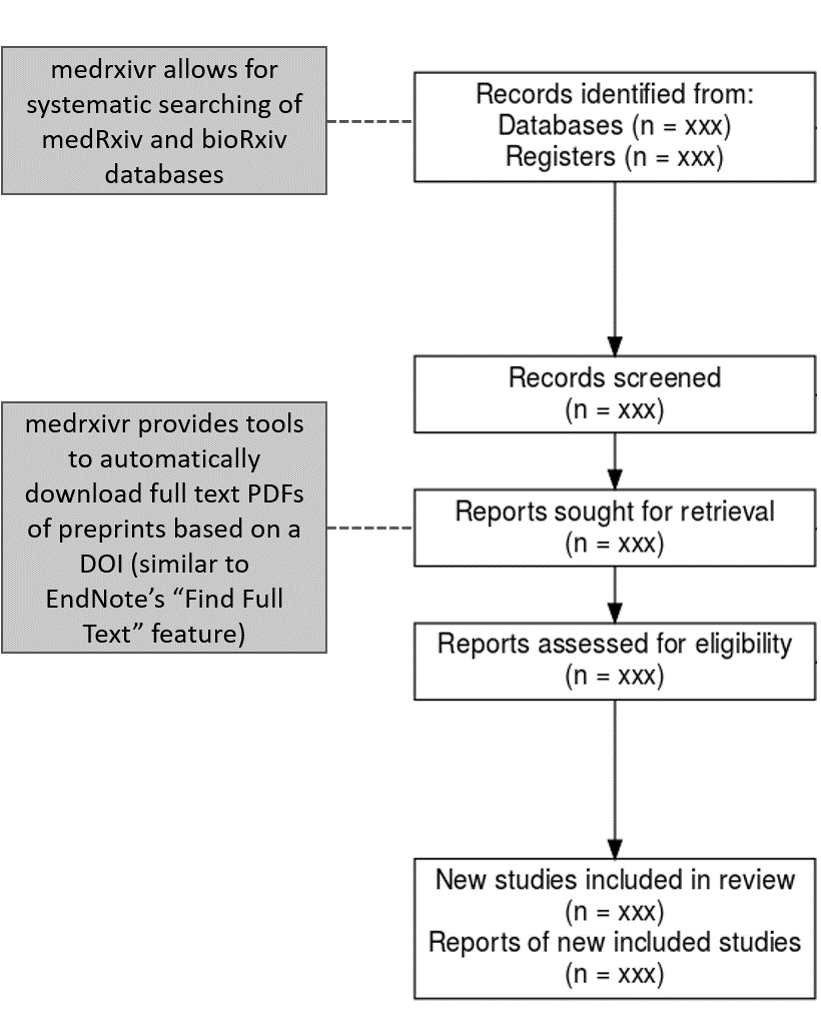
\includegraphics[width=0.65\linewidth]{figures/sys-rev-tools/medrxiv-role} 

}

\caption[Role of \texttt{medrxivr} in a systematic review workflow]{\textbf{Role of \texttt{medrxivr} in a systematic review workflow} - \texttt{medrxivr} allows for systematic searching of biomedical preprints as part of the initial literature searching. Following title and abstract screening, reviewers can then programmatically retrieve a copy of the PDF of included records to facilitate the full-text screening stage (similar to Endnote's ``Find Full Text'' feature).}\label{fig:medrxivr-sr}
\end{figure}

\hypertarget{development}{%
\section{Development}\label{development}}

\hypertarget{success-criteria}{%
\subsection{Success criteria}\label{success-criteria}}

I developed the tool to meet three success criteria,\textsuperscript{\protect\hyperlink{ref-wateridge1995}{106}} influenced both by the functionality required to perform systematic searches as part of the review in Chapter \ref{sys-rev-heading}, discussion with information specialist colleagues, and an informal survey of the evidence synthesis and health librarian communities on Twitter. The criteria were as follows:

\begin{enumerate}
\def\labelenumi{\arabic{enumi}.}
\item
  reliable, reproducible and transparent search functionality, allowing for Boolean (AND/OR/NOT) operator logic;
\item
  support for bulk export of references returned by the search to a file type that can be readily imported into a reference manager (e.g., \emph{.bib} or \emph{.ris}); and
\item
  automated retrieval of the full-text PDFs of relevant records, similar to the Find Full Text feature offered by EndNote.
\end{enumerate}

~

\hypertarget{alternative-medrxivbiorxiv-interfaces}{%
\subsection{Alternative medRxiv/bioRxiv interfaces}\label{alternative-medrxivbiorxiv-interfaces}}

Prior to development of this tool, I conducted an audit of existing tools for accessing medRxiv and bioRxiv metadata. While none address the success criteria described above, two of these tools are useful to consider to highlight the additional functionality that \texttt{medrxivr} contributes.

The first, a platform called Rxivist\textsuperscript{\protect\hyperlink{ref-abdill2019}{107}}, allows users to search preprints using keywords. However, the core functionality of the Rxivist platform is focused around exploring the number of times a preprint has been downloaded and/or shared on Twitter, to allow researchers to find the most popular papers related to their topic. The search interface\textsuperscript{\protect\hyperlink{ref-zotero-15027}{108}} does not allow for complex search strategies using Boolean operators and there is no option to batch-export the results of a search.

The second tool, \texttt{search.bioPreprint}, allows users to search for terms across a range of preprint servers, including medRxiv and bioRxiv, but also journals which use a post-publication peer-review process such as F1000Research.\textsuperscript{\protect\hyperlink{ref-iwema2016}{109}} However, similar to the Rxivist platform, this tool is designed for researchers aiming to keep up to date with recent developments in their fields rather than systematically assess the entirety of the available literature. As such, the platform only returns the most recent 1,000 records by publication date.

Finally, neither tool provides an easy way to programmatically download a copy of the PDF of relevant preprints as part of the preparation for the full-text screening stage of a systematic review.

~

\hypertarget{early-versions}{%
\subsection{Early versions}\label{early-versions}}

Work on the \texttt{medrxivr} tool began in Summer 2019, and initially consisted of a development of set of R scripts to allow for searching medRxiv and bioRxiv as part of the systematic search outlined in Chapter \ref{sys-rev-heading}. Following interest from other researchers in using the \emph{ad-hoc} web-scraping scripts, additional development work took place in 2019/2020, allowing for improved searching and exporting functionality and I released the initial version of the \texttt{medrxivr} R package in February 2020.

Early versions of the tool had a reliance on scraping data directly from the repository website. Web-scraping is a fragile mechanism for extracting data, as it is entirely dependent on consistent website design and underlying code structure remaining unchanged.\textsuperscript{\protect\hyperlink{ref-shaw2002}{110},\protect\hyperlink{ref-laprie1992}{111}}. In the case of \texttt{medrxivr}, as the medRxiv/bioRxiv websites are regularly updated, ensuring the web-scraping performed as expected required me to regularly update or fix the script.

However, an Application Programming Interface (API) for the medRxiv and bioRxiv repositories was made public in early 2020 by the institution responsible for managing these preprint repositories, the Cold Springs Harbor Laboratory. This allowed for newer versions of the \texttt{medrxivr} package to engage in active ``fault prevention'' and provide a more robust interface to the data by removing the reliance of web-scraping.\textsuperscript{\protect\hyperlink{ref-laprie1992}{111}}

~

\hypertarget{package-infrastructure}{%
\subsection{Package infrastructure}\label{package-infrastructure}}

I wrote the \texttt{medrxvir} package in R using RStudio,\textsuperscript{\protect\hyperlink{ref-rcoreteam2019}{112}} and followed development best-practice, including development of detailed documentation, a robust unit testing framework (99\% of all code lines within the package are formally tested across multiple platforms including Windows, MacOS, and Linux), and in-depth code review by two experienced, independent reviewers.

~

\hypertarget{usage}{%
\section{Usage}\label{usage}}

The \texttt{medrxivr} R package is split into two component parts:

\begin{itemize}
\tightlist
\item
  an interface to the Cold Springs Harbor Laboratory API, which imports medRxiv and bioRxiv metadata into R; and
\item
  a collection of functions for working with the imported metadata, with an explicit focus on searching this data as part of a systematic review or evidence synthesis project.
\end{itemize}

The standard workflow is to download a copy of all metadata contained in the repository, and then to perform searches on this local copy. This is a workaround as the Cold Springs Harbor Laboratory API does not provide any functionality to search the database.

While the package allows users to interact with and search both medRxiv and bioRxiv metadata, as the process is identical for both, searching the medRxiv database is used as an illustrative example throughout this chapter.

~

\hypertarget{installation}{%
\subsection{Installation}\label{installation}}

\texttt{medrxivr} has been released to the Comprehensive R Archive Network (CRAN), and can be installed with the following code:

~

\begin{Shaded}
\begin{Highlighting}[]
\FunctionTok{install.packages}\NormalTok{(}\StringTok{"medrxivr"}\NormalTok{)}
\end{Highlighting}
\end{Shaded}

~

Alternatively, the development version of the package can be installed from GitHub:

~

\begin{Shaded}
\begin{Highlighting}[]
\CommentTok{\# install.packages("devtools") }
\NormalTok{devtools}\SpecialCharTok{::}\FunctionTok{install\_github}\NormalTok{(}\StringTok{"ropensci/medrxivr"}\NormalTok{)}
\end{Highlighting}
\end{Shaded}

~

\hypertarget{importing-preprint-metadata}{%
\subsection{Importing preprint metadata}\label{importing-preprint-metadata}}

Prior to searching the metadata, it must first be imported in R. In \texttt{medrixvr}, I have provided two separate but related methods for users to import the data (Figure \ref{fig:medrxivr-data-sources}). The first of these methods, accessed via the \texttt{mx\_api\_content()} function, creates a local copy of all data available from the medRxiv API at the time the function is run.

~

\begin{Shaded}
\begin{Highlighting}[]
\CommentTok{\# Get a copy of the database from the live medRxiv API endpoint}
\NormalTok{mx\_data }\OtherTok{\textless{}{-}} \FunctionTok{mx\_api\_content}\NormalTok{()}
\end{Highlighting}
\end{Shaded}

~

This provides an up-to-the-minute reflection of the medRxiv preprint repository. However, this approach has two limitations. Firstly, as the API returns results as a series of pages limited to 100 records per page, downloading the entire database requires a time-intensive process of cycling through multiple pages. Secondly, the API can become unavailable, either during peak usage times or planned maintainence windows.

To address these limitations, I provide a second method of accessing medRxiv data, called via the \texttt{mx\_snapshot()} function, which allows users to access a maintained static snapshot of the database.

~

\begin{Shaded}
\begin{Highlighting}[]
\CommentTok{\# Import a copy of the medRxiv data from the snapshot}
\NormalTok{mx\_data }\OtherTok{\textless{}{-}} \FunctionTok{mx\_snapshot}\NormalTok{()}
\end{Highlighting}
\end{Shaded}

~

This snapshot is created each morning at 6am using a process known as ``git-scraping'',\textsuperscript{\protect\hyperlink{ref-zotero-15031}{113}} whereby the entire database is downloaded using the \texttt{mx\_api\_content()} function and saved as a comma separated value (CSV) file to an online server (Figure \ref{fig:medrxivr-data-sources}). Calling \texttt{mx\_snapshot()} imports this CSV into R, and has the advantage of both faster loading of the data into R (as it is imported as a single file and does not require cycling through the output of the API) and an absence of any reliance on the API.

The one limitation of this approach is that the snapshot (by its nature) will not contain details of records added to the database since it was taken. However, given that the number of records added each day is relatively low, this should pose minor issues.

~





\begin{figure}[H]
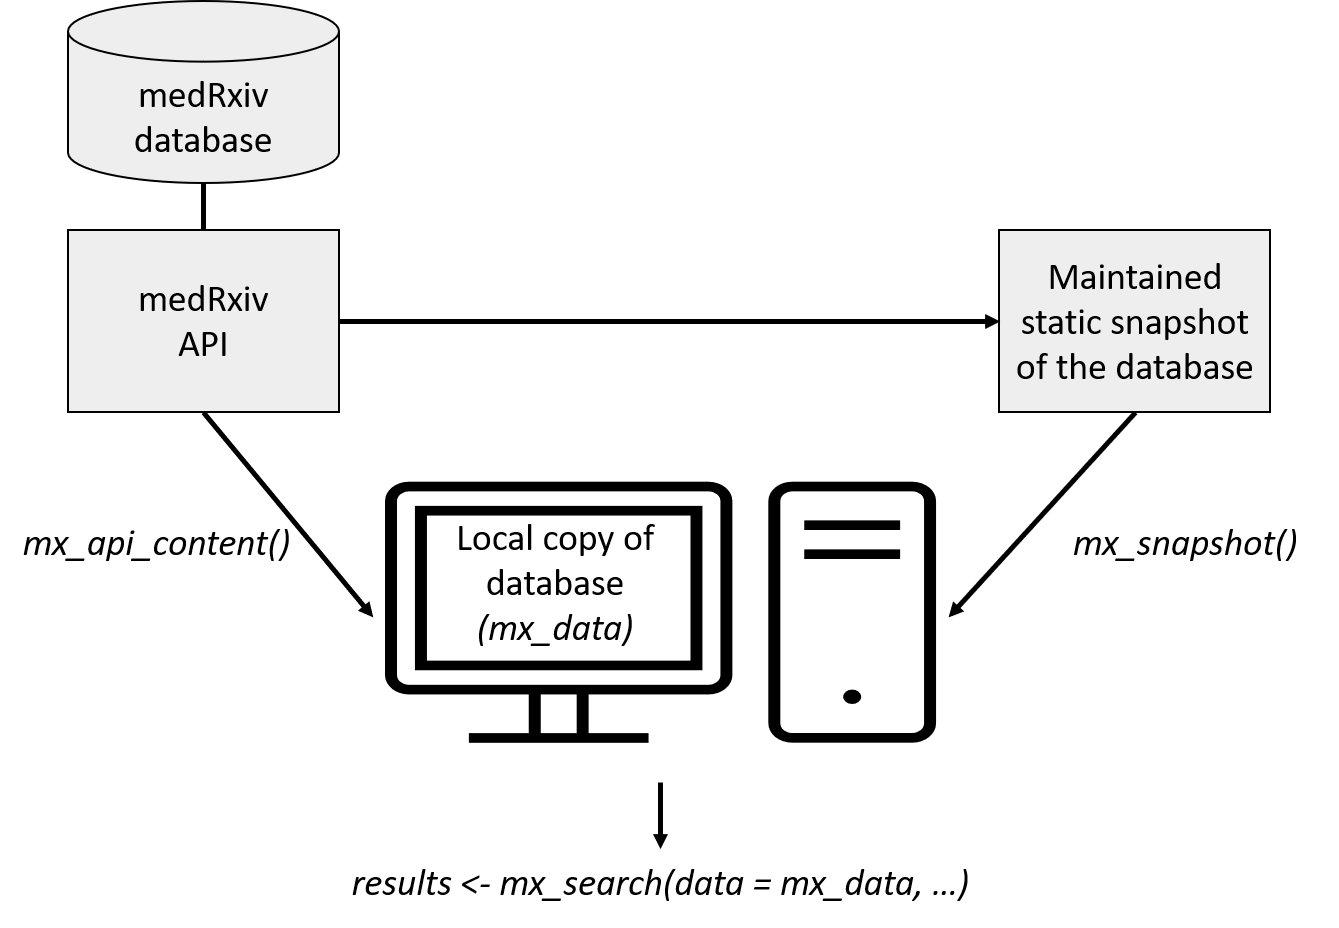
\includegraphics[width=1\linewidth]{figures/sys-rev-tools/data_sources} \caption[Overview of \texttt{medrxivr} data sources]{\textbf{Overview of \texttt{medrxivr} data sources} - Users can either access the API directly via \texttt{mx\_api\_content()}, or can import a maintained snapshot of the database, taken each morning at 6am, via the \texttt{mx\_snapshot()} function. Note: due to the size of bioRxiv, only a maintained snapshot of the medRxiv repository is available via \texttt{mx\_snapshot()}.}\label{fig:medrxivr-data-sources}
\end{figure}

~

~

\hypertarget{performing-a-search}{%
\subsection{Performing a search}\label{performing-a-search}}

Once a local copy of the metadata is created, the first step in searching it is to create a search strategy. Search terms to be combined with the OR operator are contained in vectors (\texttt{c(...)}), while topics to be combined with the AND operator are contained in lists (\texttt{list(...)}).

~

\begin{Shaded}
\begin{Highlighting}[]
\CommentTok{\# Create the search query}
\NormalTok{topic1  }\OtherTok{\textless{}{-}} \FunctionTok{c}\NormalTok{(}\StringTok{"dementia"}\NormalTok{,}\StringTok{"alzheimer\textquotesingle{}s"}\NormalTok{)  }\CommentTok{\# Combined with OR}
\NormalTok{topic2  }\OtherTok{\textless{}{-}} \FunctionTok{c}\NormalTok{(}\StringTok{"lipids"}\NormalTok{,}\StringTok{"statins"}\NormalTok{)        }\CommentTok{\# Combined with OR}

\NormalTok{myquery }\OtherTok{\textless{}{-}} \FunctionTok{list}\NormalTok{(topic1, topic2)         }\CommentTok{\# Combined with AND}
\end{Highlighting}
\end{Shaded}

~

For example, when written in standard syntax, the search contained in the \texttt{myquery} object above would be: ``((dementia \textbf{OR} alzheimer's) \textbf{AND} (lipids \textbf{OR} statins))''. There is no limit to the number of search terms that can be included in each topic, nor in the number of topics that can be search for. Search terms can also contain common syntax used by systematic reviewers and health librarians, including the use of NEAR statements which allows for identification of co-localised terms, and wild-cards, which allow for alternate spellings, e.g.~``randomi\emph{s}ation'' vs ``randomi\emph{z}ation''.

Once a strategy has been defined, it is passed along with the local copy of the database to the \texttt{mx\_search()} function.

~

\begin{Shaded}
\begin{Highlighting}[]
\CommentTok{\# Run the search}
\NormalTok{results }\OtherTok{\textless{}{-}} \FunctionTok{mx\_search}\NormalTok{(mx\_data,}
\NormalTok{                     myquery)}
\end{Highlighting}
\end{Shaded}

~

\hypertarget{refining-a-search}{%
\subsection{Refining a search}\label{refining-a-search}}

An important argument of the \texttt{mx\_search()} is \texttt{report}, which outputs a structured table with each search strategy presented on an individual line and the number of records associated with this strategy.\textsuperscript{\protect\hyperlink{ref-rethlefsen2021prisma}{114}}

~

\begin{Shaded}
\begin{Highlighting}[]
\NormalTok{results  }\OtherTok{\textless{}{-}} \FunctionTok{mx\_search}\NormalTok{(mx\_data,}
\NormalTok{                      myquery,}
                      \AttributeTok{report =} \ConstantTok{TRUE}\NormalTok{)}
\end{Highlighting}
\end{Shaded}

\begin{Shaded}
\begin{Highlighting}[]
\DocumentationTok{\#\# Found 1 record(s) matching your search.}
\DocumentationTok{\#\# }
\DocumentationTok{\#\# Total topic 1 records: 224}
\DocumentationTok{\#\# dementia: 224}
\DocumentationTok{\#\# alzheimer\textquotesingle{}s: 0}
\DocumentationTok{\#\# }
\DocumentationTok{\#\# Total topic 2 records: 119}
\DocumentationTok{\#\# lipids: 90}
\DocumentationTok{\#\# statins: 33}
\end{Highlighting}
\end{Shaded}

~

This allows users to discover which terms in their search are contributing most to the total number of results returned. This is important as part of developing a search strategy,\textsuperscript{\protect\hyperlink{ref-bramer2018}{115}} as it allows for the key terms related to each topic to be discovered. It also aids in identifying misspelled or case-sensitive search terms, which will frequently return no results. As an example, in the search presented above, the term ``alzheimer's'' returns no records. This is expected, as ``Alzheimer'' is a proper noun and so should be capitalised, but serves to illustrate the usefulness of the reporting function.

~

\hypertarget{exporting-to-a-bibliography-file}{%
\subsection{Exporting to a bibliography file}\label{exporting-to-a-bibliography-file}}

In line with my second success criteria (Section \ref{success-criteria}), one of the key features of the \texttt{medrxivr} is the ability for users to easily export the results of their systematic search to a reference manager. While it is a seemingly simple request, this is is one of the key ways in which \texttt{medrxivr} is set apart for other preprint search tools, including the native medRxiv/bioRxiv website search functionality.

For example, the results of our simple search above can be exported to the \texttt{"medrxiv\_export.bib"} file using the following code:

~

\begin{Shaded}
\begin{Highlighting}[]
\FunctionTok{mx\_export}\NormalTok{(results, }
          \AttributeTok{file =} \StringTok{"medrxiv\_export.bib"}\NormalTok{,}
          \AttributeTok{report =} \ConstantTok{TRUE}\NormalTok{)}
\end{Highlighting}
\end{Shaded}

~

\hypertarget{downloading-the-pdfs-of-relevant-records}{%
\subsection{Downloading the PDFs of relevant records}\label{downloading-the-pdfs-of-relevant-records}}

\texttt{medrxivr} alos allows users to download the full text papers for records that are deemed eligible for full-text screening (see Figure \ref{fig:medrxivr-sr}). \texttt{mx\_download()} takes the list of included records and saves the PDF for each to a folder specified by the user. This functionality is similar to the ``Find Full Text'' feature offered by EndNote.

~

\begin{Shaded}
\begin{Highlighting}[]
\FunctionTok{mx\_download}\NormalTok{(results,  }\CommentTok{\# Search results, less excluded records}
            \StringTok{"pdf/"}\NormalTok{)   }\CommentTok{\# Directory to save PDFs to }
\end{Highlighting}
\end{Shaded}

~

\hypertarget{discussion}{%
\section{Discussion}\label{discussion}}

\hypertarget{reception-and-future-plans}{%
\subsection{Reception and future plans}\label{reception-and-future-plans}}

The tool has been well received by the community (as of December 2021, \texttt{medrxivr} has been downloaded more than 5900 times), and several use cases have been reported. It has been used to investigate the role of preprints in the response to the 2019 coronavirus outbreak,\textsuperscript{\protect\hyperlink{ref-kodvanj2020}{116}} perform searches of preprints as part of a systematic review,\textsuperscript{\protect\hyperlink{ref-noone2020}{117},\protect\hyperlink{ref-grassly2020}{118}} and examine how data-sharing behaviour is affected by journal policies (see \ref{thesis-output}).\textsuperscript{\protect\hyperlink{ref-mcguinness2020c}{\textbf{mcguinness2020c?}}}

The package has been accepted into the rOpenSci suite of packages, a collection of ``carefully vetted, staff- and community-contributed R software tools that lower barriers to working with scientific data sources on the web''.\textsuperscript{\protect\hyperlink{ref-boettiger2015}{119}} As part of this process, following rigorous peer-review, an associated article introducing the tool was published by the Journal of Open Source Software.\textsuperscript{\protect\hyperlink{ref-mcguinness2020a}{\textbf{mcguinness2020a?}}} The entire review discussion is publicly available and can be viewed online.\textsuperscript{\protect\hyperlink{ref-zotero-15016}{120}} The tool has also been well received by the open-source community, demonstrated by the engagement of other developers in contributing to important new functionality and suggesting bug-fixes.

Lobbying of the Cold Springs Harbor Laboratory to develop the API to allow for direct searching of the database has been ongoing. This would negate the current need to download a local copy of the relevant preprint database before searching it, which is currently the rate limiting step for performing searches. For example, as of January 2021, downloading a copy of the bioRxiv database takes approximately an hour.

~

\hypertarget{use-cases}{%
\subsection{Use cases}\label{use-cases}}

In addition to being used to search systematically search health-related preprint servers, as illustrated in the systematic review presented in Chapter \ref{sys-rev-heading}, \texttt{medrxivr} has other uses.

For example, I led a descriptive analysis of the change in data availability statements between preprinted and published versions of the same manuscript, stratified by journal data sharing policy access, underpinned by preprint meta-data provided by \texttt{medrixvr}. By comparing the preprinted and published versions of the data availability statement, I could examine the same manuscript (same content, authors and funders) under two different publication policies, and examine whether stricter policies which require data sharing as a condition of publication actually result in increased data availability. We found some evidence that data availability statements more frequently described open data on publication when the journal mandated data sharing compared to when the journal did not mandate data sharing. This study has since been published in PLOS One, and a copy is included in Appendix \ref{published-papers}.

Secondly, using \texttt{medrxivr}, an analysis of the publication rate for medRxiv preprints was performed (see Appendix \ref{appendix-sys-rev-tools}). Eighty-seven (67.4\%) of the 129 records posted on medRxiv in July 2019 were published by 30th July 2021 (i.e.~allowing for a two-year lag between preprint posting and publication). This finding agrees with previous work demonstrating that two-thirds of bioRxiv preprints are published in a peer-reviewed journal within two years of posting,\textsuperscript{\protect\hyperlink{ref-abdill2019b}{121}} indicating that a non-insignificant number of preprints are never formally published but remain accessible as preprints.

In short, these use cases illustrate that easy access to medRxiv/bioRxiv metadata has applications beyond systematic searching of preprints by enabling meta-research/methodological analyses.

\hypertarget{medrxivr-limitations}{%
\subsection{\texorpdfstring{Limitations of \texttt{medrxivr}}{Limitations of medrxivr}}\label{medrxivr-limitations}}

While searching of the medRxiv and bioRxiv databases was crucial for the systematic review element of my thesis presented in Chapter \ref{sys-rev-heading}, there are some important limitations to note here. A key example is that the tool only searches the available metadata of preprint records (the title, abstract and keywords), rather than the full text of preprints, meaning some relevant records might be missed. However, this approach echoes that used by other search platforms such as OvidSP, and while some relevant records may be missed (reduced sensitivity), limiting the search to the metadata fields prevents non-relevant records from being returned (high specificity). A key example of the reduced specificity when searching the full text, identified during development of \texttt{medrxivr}, is that a search for ``dementia'' would return a record where the only occurrence of this term is in the title of one of the references.\textsuperscript{\protect\hyperlink{ref-bong2019}{122}}

There is also the potential that the cross-section of literature posted on medrxiv/bioRxiv is substantially different those suffering from publication bias (studies or analyses that are not published for a range of reasons including results that are not deemed ``novel'' or are not statistically significant).\textsuperscript{\protect\hyperlink{ref-song2010}{123}} This is because simply lowering the barriers to publication may well encourage authors to published ``null'' results, but due to the effort involved in writing up a distributable manuscript, it is unlikely to completely address the ``file drawer'' effect.\textsuperscript{\protect\hyperlink{ref-rosenthal1979}{76}}

It is likely too early (and likely too methodologically difficult) to tell whether the increased popularity and acceptance of preprint repositories will have any effect of the availability of research that was not considered ``publishable'' at other venues.

~

\hypertarget{role-of-open-source-tools-in-evidence-synthesis}{%
\subsection{Role of open source tools in evidence synthesis}\label{role-of-open-source-tools-in-evidence-synthesis}}

Part of the motivation for creating the \texttt{medrxivr} tool was a belief that the development and distribution of open source scripts and tools should be a fundamental part of evidence synthesis research.\textsuperscript{\protect\hyperlink{ref-goldacre2019b}{\textbf{goldacre2019b?}},\protect\hyperlink{ref-mckiernan2016c}{\textbf{mckiernan2016c?}}} In the case of \texttt{medrxivr}, it is likely that several other evidence synthesists had written personal scripts that have a similar, or related, functionality - in fact, following development of the tool, I identified one other researcher that has done so (Nicholas Fraser, author of the \texttt{rbiorxiv} package, which allows for importing medRxiv metadata into R but does not provide search functionality).\textsuperscript{\protect\hyperlink{ref-rbiorxiv}{\textbf{rbiorxiv?}}} If these scripts continue to be developed in private and are never shared or publicised, this will inevitably hamper the efforts of evidence synthesis community, not only in terms of duplication of time and effort but also due to lost opportunities for collaboration.\textsuperscript{\protect\hyperlink{ref-mckiernan2016c}{\textbf{mckiernan2016c?}}} Creating and sharing well-documented packages, the recognised standard for sharing code in R, represents one way to reduce this inefficiency.\textsuperscript{\protect\hyperlink{ref-vuorre2020}{124}}

\hypertarget{summary-1}{%
\section{Summary}\label{summary-1}}

\begin{itemize}
\item
  In this Chapter, I have introduced a new tool, \texttt{medrxivr}, for performing complex systematic searches of the medRxiv and bioRxiv preprint repositories.
\item
  I have outlined the motivation for developing this tool in relation to this thesis - more specifically, that it was used to perform systematic and reproducible searches of a key literature sources used in the comprehensive systematic review described in Chapter \ref{sys-rev-heading}.
\item
  I have contrasted \texttt{medrxivr} with other available interfaces to medRxiv/bioRxiv data to highlight the added functionality it offers. I have also discussed the tools reception to date, its limitations, and the important role of open-source tools like \texttt{medrxivr} in evidence synthesis.
\end{itemize}

\newpage

\hypertarget{references-1}{%
\section{References}\label{references-1}}



\hypertarget{sys-rev-methods-heading}{%
\chapter{Systematic review of all available evidence on the association between blood lipids and dementia outcomes}\label{sys-rev-methods-heading}}

\minitoc 

\hypertarget{lay-summary-2}{%
\section{Lay summary}\label{lay-summary-2}}

Systematic reviews are a type of research study that aim to collect and combine all existing evidence to provide the best possible answer to an important research question. Well-performed reviews involve multiple steps including: searching of existing studies; assessment of the studies against predefined inclusion criteria; collection of data from each study; and assessment of each study's methods.

This chapter presents a systematic review of primary studies that have examined the relationship between the levels of blood lipids (such as cholesterol and triglycerides), and treatments that change these levels such as statins, and dementia outcomes.

My review included 81 primary studies that contained information on this relationship. I found that statins appear to reduce the risk of Alzheimer's disease, but had no effect of vascular dementia. Lipid levels were not associated with any outcome. The methods used in some of the primary studies meant that I was less confident in the accuracy of their results.

The added value of including preprinted study reports, made possible using the tool described in the previous chapter, along with the use of the results of this review in subsequent chapters, is discussed.

~

\hypertarget{sys-rev-intro}{%
\section{Introduction}\label{sys-rev-intro}}

In this chapter, I describe a comprehensive systematic review of the relationship between blood lipid levels, and treatments that modify them, and the subsequent risk of dementia and related outcomes.

This analysis sought to address two specific aims. Firstly, as discussed in the Introduction to this thesis (Section \ref{evidence-association}), several diverse forms of evidence on the relationship of lipids and dementia exist. These include randomised controlled trials, observational studies of different analytical design, and Mendelian randomisation studies. However, based on a scoping review of existing literature, no previous evidence synthesis exercise has attempted to examine the association of lipids/statins with dementia outcomes across these distinct evidence types. Collating these diverse evidence sources is important, as if the observed association between lipids and dementia is constant across them, it increases our confidence in the association. As such, the primary aim of this analysis was to systematically review all available literature describing prospective analyses, regardless of study design.

Secondly, I explicitly sought to include health-related preprint servers as a potential evidence source in this review, as they are infrequently considered by evidence synthesists but report relevant unpublished analyses. As a sensitivity analysis to this review presented in this chapter, I sought to quantify the additional evidential value of including preprints, making use of the preprint search tool presented in Chapter \ref{sys-rev-tools-heading}.

The results of this review are used to guide the primary analysis presented in Chapter \ref{cprd-analysis-heading} and \ref{ipd-heading}, in addition to forming a key evidence source used in the triangulation exercise presented in Chapter \ref{tri-heading}.

~

\hypertarget{methods}{%
\section{Methods}\label{methods}}

\hypertarget{protocol}{%
\subsection{Protocol}\label{protocol}}

A pre-specified protocol for this analysis was registered on the Open Science Framework platform and is available for inspection.\textsuperscript{\protect\hyperlink{ref-mcguinnessluke2020}{126}} Deviations from this protocol are detailed in the relevant sections.

~

\hypertarget{contributions}{%
\subsection{Contributions}\label{contributions}}

In line with best-practice guidance, secondary reviewers were used to check the accuracy of screening, data extraction and risk-of-bias assessment processes. Due to the scale of the project, this review was performed in conjunction with a team of secondary reviewers (see Acknowledgements and Author Declaration in the front matter).

~

\hypertarget{search-strategy}{%
\subsection{Search strategy}\label{search-strategy}}

I systematically searched several electronic bibliographic databases to identify potentially relevant entries (hereafter referred to as ``records''). The following databases were searched from inception onwards: Medline, EMBASE, Psychinfo, Cochrane Central Register of Controlled Trials (CENTRAL), and Web of Science Core Collection. As the contents of the Web of Science Core Collection can vary by institution,\textsuperscript{\protect\hyperlink{ref-gusenbauer2020a}{127}} the specific databases and date ranges for each database searched via this platform are listed in Appendix \ref{appendix-wos-databases}. The search strategy used in each database was developed in an iterative manner using a combination of free text and controlled vocabulary (MeSH/EMTREE)\textsuperscript{\protect\hyperlink{ref-lefebvre2019searching}{72}} terms to identify studies which have examined the relationship between blood lipids levels and dementia, incorporating input from an information specialist. The strategy included terms related to lipids, lipid modifying treatments, and dementia, and was designed for MEDLINE before being adapted for use in the other bibliography databases listed. A high-level outline of the strategy is presented in the Table \ref{tab:searchOverview-table} below and the full search strategies for each database are presented in Appendix \ref{appendix-search-strategy}.

~





\begin{table}[H]

\caption[searchOverview]{\label{tab:searchOverview-table}Summary of systematic search by topic. The full search strategy including all terms and the number of hits per term is included in Appendix \ref{appendix-search-strategy}.}
\centering
\fontsize{10}{12}\selectfont
\begin{threeparttable}
\begin{tabular}[t]{>{}cl}
\toprule
\textbf{No.} & \textbf{Concept}\\
\midrule
1 & Dementia\\
\midrule
2 & Lipids\\
\midrule
3 & Lipid-modifying treatments\\
\midrule
4 & 1 AND 2\\
\midrule
5 & 1 AND 3\\
\midrule
\addlinespace
6 & 4 OR 5\\
\midrule
7 & Animals NOT (Animals AND Humans)\\
\midrule
8 & 6 NOT 7\\
\midrule
9 & Observational filter\\
\midrule
10 & Randomised controlled trial (RCT) filter\\
\midrule
\addlinespace
11 & Mendelian randomisation/Instrumental variable filter\\
\midrule
12 & OR/ 9-11\\
\midrule
13 & 8 AND 12\\
\bottomrule
\end{tabular}
\begin{tablenotes}
\item For all topics, search queries were comprised of relevant free text \& controlled vocabulary terms.
\end{tablenotes}
\end{threeparttable}
\end{table}

~

When searching the bibliographic databases, study design filters were employed to try and reduce the screening load. To ensure that the study design filters were not excluding potentially relevant records, a random sample of 500 records identified by the main search but excluded by the filters (defined as ``8 NOT 12'' in Table \ref{tab:searchOverview-table}) was screened.

I also searched clinical trial registries, for example ClinicalTrials.gov, to identify relevant randomized controlled trials. In addition, I searched the bioRxiv and medRxiv preprint repositories using the tool developed in Chapter \ref{sys-rev-tools-heading} to identify potentially relevant preprinted studies (see Appendix \ref{appendix-medrxivr-code} for the code used to search these preprint repositories).

Grey literature was searched via ProQuest, OpenGrey and Web of Science Conference Proceedings Citation Index, while theses were accessed using the Open Access Theses and Dissertations portal. In addition, the abstracts list of relevant conferences (e.g.~the proceedings of the Alzheimer's Association International Conference, published in the journal Alzheimer's \& Dementia) were searched by hand. Finally, the reference lists of included studies were searched by hand while studies citing included studies was examined using Google Scholar (forward and reverse citation searching or ``snowballing'').

~

\hypertarget{study-selection}{%
\subsection{Study selection}\label{study-selection}}

Records were imported into Endnote and de-duplicated using the method outlined in Bramer et al.~(2016).\textsuperscript{\protect\hyperlink{ref-bramer2016}{128}} In summary, this method uses multiple stages to identify potential duplicates, beginning with automatic deletion of records matching on multiple fields (``Author'' + ``Year'' + ``Title'' + ``Journal''), followed by manual review of less similar articles (e.g.~those identified as duplicates based on the ``Title'' field alone).

Following de-duplication of records, screening (both title/abstract and full-text) was performed using a combination of Endnote, a citation management tool,\textsuperscript{\protect\hyperlink{ref-hupe2019}{129}} and Rayyan, a web-based screening application.\textsuperscript{\protect\hyperlink{ref-ouzzani2016}{130}} Title and abstract screening to remove obviously irrelevant records was performed primarily by me, with a random \textasciitilde10\% sample of excluded records being screened in duplicate to ensure consistency with the inclusion criteria. Additionally, I re-screened the same \textasciitilde10\% sample with 3 month lag to assess intra-rater consistency.

Similarly, I completed all full-text screening, with a random \textasciitilde20\% being screened in duplicate by a second reviewer, in addition to any records identified I identified as being difficult to assess against the inclusion criteria were screened in duplicate. Reasons for exclusion at this stage were recorded. Disagreements occurring during either stage of the screening process were resolved through discussion with a senior colleague. A PRIMSA flow diagram was produced to document how records moved through the review.\textsuperscript{\protect\hyperlink{ref-page2021}{83}}

The criteria against which records were assessed for eligibility are presented in the subsequent sections.

~

\hypertarget{inclusion-criteria}{%
\subsubsection{Inclusion criteria}\label{inclusion-criteria}}

I sought to include studies that examined blood lipid levels as a risk factor for demenita outcomes, defined either as binary hypercholesterolemia variable or by category/1-standard-deviation increase of a specific lipid fraction (total cholesterol, high- and low-density lipoprotein cholesterol and triglycerides). I also aimed to include studies examining the effect of treatments that modify lipids levels as a source of indirect evidence. Eligible study designs included randomized controlled trials and non-randomized observational studies of lipid modifying treatments, longitudinal studies examining the effect of increased/decreased blood lipid levels, and genetic instrumental variable (Mendelian randomization) studies examining the effect of genetically increased/decreased blood lipid levels.

Eligible studies screened participants for dementia at baseline and excluded any prevalent cases. Alternatively, where no baseline screening was employed, participants were assumed to be dementia free if less than 50 years of age at baseline. Studies of any duration were included to allow for exploration of the effect of length of follow-up on the effect estimate using meta-regression. No limits were placed on the sample size of included studies.

Eligible studies defined dementia outcomes according to recognised criteria, for example the International Classification of Diseases (ICD),\textsuperscript{\protect\hyperlink{ref-organizationwho1993}{131}} National Institute of Neurological Disorders and Stroke Association-Internationale pour la Recherche en l'Enseignement en Neurosciences (NINDS-AIREN),\textsuperscript{\protect\hyperlink{ref-roman1993}{132}} or Diagnostic and Statistical Manual of Mental Disorders (DSM) criteria.\textsuperscript{\protect\hyperlink{ref-edition2013}{133}} Studies utilising electronic health records were the exception to this, as it was assumed that a valid criteria was employed when entering used when entering the outcome into the EHR.

Conference abstracts with no corresponding full-text publication were eligible, and where required, I contacted authors to obtain information on the study's status. No limitations were imposed on publication status, date, venue or language.

~

\hypertarget{exclusion-criteria}{%
\subsubsection{Exclusion criteria}\label{exclusion-criteria}}

Due to the significant impact of a memory-related outcome such as dementia on exposure recall, case-control studies were excluded, though nested case-control studies, where historical records are used to determine the exposure status, were eligible for inclusion. Cross-sectional studies, qualitative studies, case reports/series and narrative reviews were also excluded, as were studies that measure change in continuous cognitive measures (e.g.~MoCA score) without attempt to map these scores to ordinal groups (e.g.~no dementia/dementia). Previous systematic reviews were not eligible for inclusion, but their reference lists were screened to identify any potentially relevant articles.

Studies with outcomes not directly related to the clinical syndrome of dementia (e.g., neuroimaging), studies implementing a ``multi-domain intervention'' where a lipid-regulating agent is included in each arms (e.g.~for example, a study examining exercise + statins vs statins alone, but a study examining exercise + statins vs exercise alone would be included), and studies where there was no screening for dementia at baseline except if the sample was initially assessed in mid-life (i.e.~below the age of 50) were excluded. Finally, studies using a dietary intervention, for example omega-3 fatty acid enriched diet, were excluded as it is difficult to disentangle the effect of other elements contained within the diet. Note, this is distinct from studies which delivered a simple tablet-based omega-3 intervention, which would have been eligible for inclusion.

~

\hypertarget{validation-of-screening-process}{%
\subsection{Validation of screening process}\label{validation-of-screening-process}}

Inter- and intra-rater reliability during the screening stages were assessed for a 10\% sub-sample of records. Intra-rater reliability involved a single reviewer applying the inclusion criteria to the same set of records while blinded to their previous decisions (i.e.~assessment of consistency), while inter-rater reliability involved two reviewers independently screening the same set of records (i.e.~assessment of accuracy).

Rater reliability was assessed using Gwet's agreement coefficient (AC1).\textsuperscript{\protect\hyperlink{ref-gwet2008}{134}} This measure was chosen over other methods such as percent agreement (number of agreements divided by total number of assessments), as it accounts for chance agreement between reviewers but does not suffer from bias due to severely imbalanced marginal totals in the same way that Cohen's \(kappa\) value does.\textsuperscript{\protect\hyperlink{ref-gwet2008}{134}} Given the small number of included studies in this review as a proportion of the total number screened, this is a useful characteristic.

How to interpret agreement co-efficients is widely debated, and while arbitary cut-off values may mislead readers,\textsuperscript{\protect\hyperlink{ref-brennan1992}{137}} they provide a useful rubric by which to assess inter-rater agreement. Here, I used guidelines based on a stricter interpretation of the Cohen's \(kappa\) coefficient,\textsuperscript{\protect\hyperlink{ref-mchugh2012}{138}} presented in Table \ref{tab:gwet-table}.

~





\begin{table}[H]

\caption[Ranges for Gwet's AC1]{\label{tab:gwet-table}Suggested ranges to aid in interpretation of Gwet's AC1 inter-rater reliability metric}
\centering
\begin{tabular}[t]{cc}
\toprule
\textbf{Kappa} & \textbf{Interpretation}\\
\midrule
0    – 0.20 & None\\
\midrule
0.21 – 0.39 & Minimal\\
\midrule
0.40 – 0.59 & Weak\\
\midrule
0.60 – 0.79 & Moderate\\
\midrule
0.80 – 0.90 & Strong\\
\midrule
\addlinespace
> 0.90 & Almost perfect\\
\bottomrule
\end{tabular}
\end{table}

~

Intra- and inter-rater reliability was assessed against these cut-offs. If this assessment demonstrated issues with the screening process (defined as an AC1 of less than .9), a larger proportion of records would have been dual-screened.

~

\hypertarget{data-extraction}{%
\subsection{Data extraction}\label{data-extraction}}

Data extraction was performed using a piloted data extraction form. Extracted items included: article metadata (year of publication, author list, journal), study characteristics (study location, data source, exposure, outcomes, outcome criteria used), patient characteristics (age, sex, baseline cognition scores, baseline education scores), and results (exposure-outcome pairing, effect measure, effect estimate, error estimate, p-value). I extracted all data in the first instance, which was subsequently checked for accuracy by a second member of the review team.

~

\hypertarget{grouping-multiple-reports-into-studies}{%
\subsubsection{Grouping multiple reports into studies}\label{grouping-multiple-reports-into-studies}}

As part of the data extraction process, multiple records resulting from the analysis of the same data were included and grouped into single units, hereafter called studies. This was common in cases where multiple papers report results on the same cohort but at different time points. This process builds out the most comprehensive account of a given studies possible by incorporating information from all available records.

This was particularly relevant to preprints and published papers reporting the same study, which were not considered to be duplicate records but instead different reports of the same study. This is due to the potential for the published version to offer some information that the preprint did not, and vice versa.

~

\hypertarget{combining-across-groups}{%
\subsubsection{Combining across groups}\label{combining-across-groups}}

In line with best practice, where summary data was presented across two groups (e.g.~age at baseline stratified by hypercholesterolemia status), the following approach was used to combine the groups:\textsuperscript{\protect\hyperlink{ref-higgins2019}{139}}

\begin{equation}
N = N_1 + N_2
  \label{eq:combiningGroups1}
\end{equation}

\begin{equation}
Mean = \frac{(N_1M_1 + N_2N_2)}{(N_1 + N_2)}
  \label{eq:combiningGroups2}
\end{equation}

\begin{equation}
SD = \sqrt{\frac{(N_1-1)SD_1^2 + (N_2-1)SD_2^2 + \frac{N_1N_2}{N_1 + N_2}(M_1^2 + M_2^2 - 2M_1M_2)}{N1 + N2 -1}}
  \label{eq:combiningGroups3}
\end{equation}

~

This was implemented in a systematic manner, with the raw group data being extracted and a cleaning script employed to combine the groups for analysis.

~

\hypertarget{harmonisation-of-cholesterol-measures}{%
\subsubsection{Harmonisation of cholesterol measures}\label{harmonisation-of-cholesterol-measures}}

Where necessary, lipid levels reported in \emph{mmol/L} were converted in \emph{mg/dL} using the following formula:

\begin{equation} 
  mg/dL = mmol/L \times{} Z
  \label{eq:lipidConversion}
\end{equation}

where \(Z = 38.67\) for total cholesterol, LDL-c and HDL-c, and \(Z = 88.57\) for triglycerides. For widely-used categorises of lipids levels on the \emph{mg/dL} scale, see Table \ref{tab:lipidLevels-table} in Section \ref{intro-lipid-fractions}.

~

\hypertarget{contacting-authors}{%
\subsubsection{Following up with authors}\label{contacting-authors}}

Where additional data points not included in the report of an analysis were required either for the analysis or risk-of-bias assessment, the corresponding author of the study was contacted. This approach was taken due to the potentially large impact of following up with authors on the results of the review.\textsuperscript{\protect\hyperlink{ref-reynders2019}{140}}

~

\hypertarget{analysis-of-varying-effect-measures}{%
\subsubsection{Analysis of varying effect measures}\label{analysis-of-varying-effect-measures}}

The range of effect measures presented by studies (odds ratios, risk ratios, hazard ratios, etc) are not directly interchangeable in the context of systematic review. As such, different effect estimates can be one potential problem that precludes a meta-analysis of all studies.\textsuperscript{\protect\hyperlink{ref-mckenzie2019}{141}} If the outcome is rare, as is the case for dementia outcomes, the estimated prevalence of odds and risk ratios will approximate each other. However, hazard ratios provide a very different interpretation, taking into account person-time-at-risk in each treatment group.

Several existing reviews do not distinguish between the types of effect measures and include all existing studies in a single meta-analysis to produce an overall effect estimate. However, in this review, the small subset of studies reporting odds/risk ratios are synthesised separately to those reporting hazard ratios.

~

\hypertarget{risk-of-bias}{%
\subsection{Risk-of-bias assessment}\label{risk-of-bias}}

A key aim of the review presented in this chapter is to identify different sources of evidence at risk of a diverse range of biases, and to contrast and compare findings across them (see Section \ref{triangulation-overview} for an overview of triangulation and Chapter \ref{tri-heading} for the results of this analysis). To enable this triangulation exercise, a detailed and structured risk-of-bias assessment formed an important part of this review.

There has been a recent movement within the evidence synthesis community away from examining \emph{methodological quality} to assessing \emph{risk of bias},\textsuperscript{\protect\hyperlink{ref-mcguinness2018}{84},\protect\hyperlink{ref-sterne2016}{142}} and thus directly evaluating the internal validity of a study. Internal validity is defined here as the absence of systematic error (or bias) in a study, which may influence its results.\textsuperscript{\protect\hyperlink{ref-campbell1957}{143},\protect\hyperlink{ref-juni2001}{144}}

This move was prompted by a unclear definition of ``methodological quality'' which could include facets such as unclear reporting, in addition to challenges in the comparison of results from different tools. As part of this shift, the focus shifted from checklist or score based tools towards domain-based methods, in which different potential sources of bias in a study are assessed in order.
Finally, the new tools tools move from assessing bias at the study level to considering separately each individual numerical result reported. For example, a study may report on the efficacy of an intervention at six months and two years follow-up. In this case, missing outcome data that is not an issue at six months may introduce bias after two years of follow-up, and assigning a single risk-of-bias judgement to the study as a whole masks the different biases applicable to each unique result.

In this review, domain-based tools were used to assess the risk of bias for each result in each included study. The study design-specific tools are introduced and discussed in more detail in the following sections.

~

\hypertarget{randomised-controlled-trials-1}{%
\subsubsection{Randomised controlled trials}\label{randomised-controlled-trials-1}}

Randomized controlled trials were assessed using the RoB 2 tool.\textsuperscript{\protect\hyperlink{ref-sterne2019}{145}} The tool assess the risk of bias across five domains: bias arising from the randomization process, bias due to deviations from intended intervention, bias due to missing outcome data, bias in measurement of the outcome, bias in selection of the reported result. Acceptable judgements for each domain include: ``low risk'', ``some concerns'', ``high risk''. Each of the five domains contains a series of signalling questions or prompts which guide the user through the tool. Once a domain-level judgement for each domain has been assigned, an overall judgement, using the same three levels of risk of bias, is assigned to the result.

~

\hypertarget{rob-tools-nrse}{%
\subsubsection{Non-randomised studies of interventions/exposures}\label{rob-tools-nrse}}

For non-randomised studies of interventions (NRSI), I used the ROBINS-I (Risk Of Bias In Non-randomised Studies - of Interventions) tool.\textsuperscript{\protect\hyperlink{ref-sterne2016}{142}} This tool assess the risk of bias across seven domains: bias due to confounding, bias due to selection of participants, bias in classification of interventions, bias due to deviations from intended interventions, bias due to missing data, bias in measurement of outcomes, and bias in selection of the reported result. Similar to RoB 2, it has a number of prompting questions per domain, with acceptable judgements including ``low risk'', ``moderate risk'', ``serious risk'' and ``critical risk''. In the context of the tool, observational studies are assessed in reference to an idealised randomised controlled trial. Under this approach, the (rare) overall judgement of ``Low'' indicates that the results should be considered equivalent to produced by a randomised controlled trial.

While a risk-of-bias tool for non-randomised studies of exposures (NRSE) is currently under development,\textsuperscript{\protect\hyperlink{ref-morganr2020}{146}} but was insufficiently developed at the time the risk-of-bias assessments for this review were performed. Instead, I used a version of the ROBINS-I tool informed by the preliminary ROBINS-E tool (Risk of Bias In Non-randomised Studies -- of Exposure), which I had previously applied in a published review.\textsuperscript{\protect\hyperlink{ref-french2019}{147}} The version had no signalling questions and so judgements, using the same four levels of bias as ROBINS-I, were made at the domain level. The motivation using this tool above other established tools such as the Newcastle-Ottowa scale (NOS)\textsuperscript{\protect\hyperlink{ref-wells2000}{148}} was two-fold. In the first instance, as mentioned in the introduction to this section, using a domain-based tool has distinct advantages over better-developed checklist-type tools including the NOS. Additionally, using a domain-based tool for non-randomised studies of exposures enabled better comparison with risk-of-bias assessments performed for the other study designs as part of this review.

~

\hypertarget{mendelian-randomisation-studies}{%
\subsubsection{Mendelian randomisation studies}\label{mendelian-randomisation-studies}}

At present, no formalised risk-of-bias assessment tool for Mendelian randomization studies is available. Assessment of the risk of bias in Mendelian randomisation studies was informed by the approach used in a previous systematic review of Mendelian randomisation,\textsuperscript{\protect\hyperlink{ref-mamluk2020}{149}} as identified by a review of risk-of-bias assessments in systematic reviews of Mendelian randomisation studies (advance results from this review were obtained from contact with the review authors).\textsuperscript{\protect\hyperlink{ref-spiga2021}{150}} A copy of this tool is available in Appendix \ref{appendix-mr-rob}, but in summary, results were assessed for bias arising from weak instruments, genetic and other confounding, pleiotropy and population stratification. Acceptable judgements for each fo the 5 domains in the tool included ``low'', ``moderate'' and ``high'' risk of bias.

~

\hypertarget{methods-rob-me}{%
\subsubsection{Risk of bias due to missing evidence}\label{methods-rob-me}}

In addition to assessing the risk of bias within each result contributing to a synthesis, I also assessed risk of bias due to missing evidence at the analysis level. This assessment examines evidence missing due to selective non-reporting - as distinct from the selective reporting of a single result from multiple planned - and was performed using the forthcoming RoB-ME (Risk of Bias due to Missing Evidence in a synthesis) tool.\textsuperscript{\protect\hyperlink{ref-zotero-15123}{151}} The tool is in development stages, and as part of this review, I piloted the tool, and provided feedback to the developers.

This additional appraisal marks a departure from the registered protocol, as there was initially no intention to try and examine the risk of bias due to missing evidence. This is largely because the tool did not exist when the protocol was registered.

~

\hypertarget{analysis-methods}{%
\subsection{Analysis methods}\label{analysis-methods}}

An inital qualiatative synthesis of evidence was performed, summarising the data extracted from studies stratified by study design. Where individual studies were deemed comparable, they were incorporated into a quantitative analysis or ``meta-analysis''.

Results were not combined across different study designs (i.e.~RCTs were not combined in a meta-analysis with results from observational studies). The summary effect estimates produced by meta-analysis of individual study designs are discussed, but are compared and contrasted more fully as part of the triangulation exercise presented in Chapter \ref{discussion-heading}.

~

\hypertarget{random-effects-meta-analysis}{%
\subsubsection{Random-effects meta-analysis}\label{random-effects-meta-analysis}}

For results examining the effect of binary or continuous exposure (as opposed to categorical/dose-response, as discussed in the next section) on any dementia outcome, a random-effects meta-analysis model was used. Random-effects meta-analysis does not assume one true underlying effect, but rather allows for a distribution of true effects with variance \(\tau^2\). The weight (\(w\)) assigned to each result (denoted as \(y_i\)) is then give as the inverse of variance of that result plus the estimate of between-result variance, denoted as \(w_i = \frac{1}{v_i+\tau^2}\) for result \(i\).

Once the weights are calculated for each result, the overall estimate (\(\hat{y}\)) and variance (\(Var(\hat{y})\)) can be estimated:

\begin{equation}
\hat{y} = \frac{\sum{y_iw_i}}{\sum{w_i}}
  \label{eq:rmaEstimate}
\end{equation}

\begin{equation}
Var(\hat{y}) = \frac{1}{\sum{w_i}}
  \label{eq:rmaVariance}
\end{equation}

~

Results were stratified into subgroups on the basis of the overall risk of bias assessment, and summary estimates for each subgroup, in addition to an overall effect estimate, are displayed in each forest plot. Additional descriptive statistics are presented, while prediction intervals are shown as a dotted line banding the overall effect estimate. Finally, where at least 10 results are available, a test subgroup differences between studies at different levels of risk of bias was performed (see subsequent Section \ref{sys-rev-visualising-results}). All models were implemented using the \texttt{metafor} R package.

~

\hypertarget{dose-response-analyses}{%
\subsubsection{Dose-response analyses}\label{dose-response-analyses}}

Several of the included studies presented data on multiple categories of lipid levels, but provided an overall effect estimate based on a comparison of only two of these categories (e.g.~for example, highest vs lowest quartile). While this allows for easy interpretation of the resulting effect estimate, it ignores any potential non-linear relationships between the exposure and outcome, in addition to discarding useful information contain in the interim groups. In order to address this limitation, I performed a dose-response meta-analysis in those studies reporting more than two categories for lipid levels. This marks a departure from the published protocol, as I was unaware that such a large number of studies would report dementia risk across multiple lipid categories.

Studies were excluded from this analysis if the number of categories was less than three or if the necessary information for synthesis (cut-off points, number of participants and number of events per category) was not available. A restricted cubic spline model was fitted to allow for a non-linear relationship, for example a U or J-shaped relationship, where low and high levels of the exposure can have different effects versus a ``normal'' reference dose. The locations of the knots in the model wer identified using fixed percentiles (25th, 50th, 75th) of the exposure data. Reference doses were defined \emph{a priori} as the cut-off of the ``Normal''/``Optimal'' categories for each fraction, as detailed in Table \ref{tab:lipidLevels-table}. Under this approach, the reference dose was defined as 200 mg/dL for total cholesterol, 100 mg/dL for LDL-c, 40 mg/dL for HDL-c, and 150 mg/dL for triglycerides.

When the highest reported category was open ended (e.g LDL-c \(\geqslant\) 200 mg/dL), I calculated the category midpoint by assuming the width of the highest category was the same as the one immediately below it. Similarly, when the lowest category was open-ended (e.g LDL-c \(\leqslant\) 100 mg/dL), I set the lower boundary for this category to zero (though this is unlikely to occur naturally).

~

\hypertarget{additional-analyses}{%
\subsubsection{Additional analyses}\label{additional-analyses}}

Where there was evidence of heterogeneity between results included in a meta-analysis, I investigated this further using meta-regression against reported characteristics. \emph{A priori}, I was interested in the effect that the age at baseline, sex and risk-of-bias judgement had on the results. Syntheses with greater than 10 studies were assessed for heterogeneity across these covariates.

Finally, I investigated the potential for small study effects, which may be caused by publication bias, both visually using funnel plots and formally using Egger's regression test.

~

\hypertarget{sys-rev-visualising-results}{%
\subsubsection{Visualisation of results}\label{sys-rev-visualising-results}}

Evidence maps are useful way to explore the distribution of research cohorts included in a systematic review.\textsuperscript{\protect\hyperlink{ref-saran2018}{152}} As part of the initial descriptive synthesis, the location of each individual study contributing to the evidence base was quantified and visualised on a world map.

One of the limitations of current risk-of-bias assessments in systematic reviews is that they are often divorced from the results to which they refer, and are infrequently incorporated into the analysis. In response to this criticism, I developed a new visualisation tool was designed to allow for the production of ``paired'' forest plots, as recommended by the ROB2 publication, where a risk-of-bias assessment is presented alongside it's corresponding numerical results.\textsuperscript{\protect\hyperlink{ref-sterne2019}{145}} This tool was developed as an adjunct to this thesis to aid in creating standardised risk-of-bias figures,\textsuperscript{\protect\hyperlink{ref-mcguinness2020robvisPaper}{153}} and the ``paired'' forest plot functionality grew out of a collaboration with other researchers to design a modular method for creating custom forest plots.\textsuperscript{\protect\hyperlink{ref-zotero-14999}{154}} A summary of this tool is contained in Appendix \ref{appendix-robvis}, and all forest plots presented in this Chapter were created using this tool.

~

\hypertarget{assessment-of-added-value-of-including-preprints}{%
\subsubsection{Assessment of added value of including preprints}\label{assessment-of-added-value-of-including-preprints}}

\emph{{[}Note: Julian, I am particularly interested in your feedback on this section, and the corresponding results section (Section \ref{sys-rev-including-preprints-res}), as I am not convinced on the language I am using{]}}

Preprints are considered a valuable evidence source within this thesis (see Introduction, Section \ref{diverse-sources-preprints}). As an adjunct analysis to this review, I explored the additional evidential value of including preprints in each meta-analysis performed, assessed using the fixed effect weight from a standard meta-analysis.

Additionally, I followed identified preprints up after a two-year lag to investigate whether they had been subsequently published (in which case preprints provide a snapshot into the future, and a systematic review update would capture these reports) or not (in which case preprints provide a distinct evidence source to conventional bibliographic databases).

~

\hypertarget{results}{%
\section{Results}\label{results}}

\hypertarget{initial-search-and-validation-of-search-filters}{%
\subsection{Initial search and validation of search filters}\label{initial-search-and-validation-of-search-filters}}

The database search identified 23,447 records, of which 7,338 were duplicated records. Of the random sample of 500 records screened to ensure the accuracy of the study design filters, no eligible records were identified. Many of those excluded by the filters were commentaries/educational articles, or described basic science studies.

~

\hypertarget{screening-results}{%
\subsection{Screening results}\label{screening-results}}

Following de-duplication, the titles and abstracts of 16,109 records were assessed for eligibility. 387 were deemed potentially eligible, and the full text records for these were accessed and screened.

The PRISMA flow diagram presented in Figure \ref{fig:prisma-flow-fig}, illustrates the movement of articles through the review. To highlight the contribution of preprint archives to the review, the flow diagram delineates between those records captured through databases searches (presented on the left of the diagram) and those captured by the search tool described in the previous chapter (presented in grey on the right of the diagram).

Common reasons for exclusion at the full text-stage included studies that reported on the wrong exposures (n = 70 ; most commonly a ineligible lipid fraction), used the wrong study design (n= 56), or reported on a wrong outcome (n=24; e.g.~change in cognitive scores).

\blandscape{}

~





\begin{figure}[H]

\includegraphics[width=1\linewidth]{figures/sys-rev/prismaflow} \caption[PRISMA flow diagram]{PRISMA flow diagram illustrating how records moved through the systematic review process. The different contributions of standard bibliographic databases and preprint servers to the review are indicated.}\label{fig:prisma-flow-fig}
\end{figure}

\elandscape{}

\hypertarget{validation-of-screening}{%
\subsection{Validation of screening}\label{validation-of-screening}}

For the assessment of the intra-/inter-rater reliability, the estimated values of \(AC1\) were interpreted against the categories presented in Table \ref{tab:gwet-table}. For the inter-rater reliability, agreement was ``almost perfect'' (\(AC1\) = 0.97, \(kappa\) = 0.54, Table \ref{tab:agreeInter-table}). Similarly for intra-rater reliability, agreement was ``almost perfect'' (\(AC1\) = 0.99, \(kappa\) = 0.65, Table \ref{tab:agreeIntra-table}). The discrepancy between the \(AC1\) and \(kappa\) coefficients illustrates the sensitivity of \(kappa\) to imbalanced marginals, caused in this sample by a large imbalance towards exclusion.\textsuperscript{\protect\hyperlink{ref-feinstein1990}{155}}

~





\begin{table}[H]

\caption[Inter-rater agreement]{\label{tab:agreeInter-table}Inter-rater agreement on a subset of records, indicating high accuracy.}
\centering
\begin{tabular}[t]{>{}l>{}lr>{}r|r}
\toprule
\multicolumn{2}{c}{ } & \multicolumn{3}{c}{Initial screening decision} \\
\cmidrule(l{3pt}r{3pt}){3-5}
\textbf{} & \textbf{} & \textbf{Exclude} & \textbf{Include} & \textbf{Total}\\
\midrule
 & \textbf{Exclude} & 1244 & 9 & 1253\\
\cmidrule{2-5}
 & \textbf{Include} & 26 & 22 & 48\\
\cmidrule{2-5}
\multirow{-3}{12em}{\raggedright\arraybackslash \textbf{Second reviewer decision}} & \textbf{Total} & 1270 & 31 & 1301\\
\bottomrule
\end{tabular}
\end{table}





\begin{table}[H]

\caption[Inter-rater agreement]{\label{tab:agreeIntra-table}Intra-rater agreement on subset of records, indicating high consistency.}
\centering
\begin{tabular}[t]{>{\raggedright\arraybackslash}p{12em}>{}lr>{}r|r}
\toprule
\multicolumn{2}{c}{ } & \multicolumn{3}{c}{Initial screening decision} \\
\cmidrule(l{3pt}r{3pt}){3-5}
\textbf{} & \textbf{} & \textbf{Exclude} & \textbf{Include} & \textbf{Total}\\
\midrule
 & \textbf{Exclude} & 1266 & 14 & 1280\\
\cmidrule{2-5}
 & \textbf{Include} & 4 & 17 & 21\\
\cmidrule{2-5}
\multirow{-3}{12em}{\raggedright\arraybackslash \textbf{Same reviewer decision (with 3 month lag)}} & \textbf{Total} & 1270 & 31 & 1301\\
\bottomrule
\end{tabular}
\end{table}

~

Those records which were excluded in the initial screening, but were included by the second reviewer (n=26, Table \ref{tab:agreeInter-table}) were investigated. This discrepancy between the two reviewers was explained in all cases by differing interpretations of the inclusion criteria, most commonly around the definition of cognitive decline versus dementia and the definition of eligible lipids fractions.

~

\hypertarget{sys-rev-characteristics}{%
\subsection{Characteristics of included studies}\label{sys-rev-characteristics}}

Following full-text screening, 81 unique studies (described across 95 reports) met the criteria for inclusion in the review.\textsuperscript{\protect\hyperlink{ref-li2005a}{49},\protect\hyperlink{ref-tan2003a}{52},\protect\hyperlink{ref-reitz2004a}{54},\protect\hyperlink{ref-heartprotectionstudycollaborativegroup2002}{156}--\protect\hyperlink{ref-zhu2018}{233}} Table \ref{tab:studyCharacteristics-table} presents a summary of the characteristics of each study.

The majority of included studies described non-randomised analyses, with the sole two included randomised controlled trials (the Heart Protection Study/British Heart Foundation trial\textsuperscript{\protect\hyperlink{ref-heartprotectionstudycollaborativegroup2002}{156}} and the JUPITER trial\textsuperscript{\protect\hyperlink{ref-ridker2008}{157}}) both reporting on the effect of statin use on all-cause dementia in older adults. A similarly small number of Mendelian randomisation studies were identified, several of which employed a two-sample approach using summary statistics from the same published genome wide association studies (GWAS) leading to complications in the synthesis (see Section \ref{sys-rev-res-AD}).

Of the 31 non-randomised studies examining treatments that modify lipid levels, all examined statin use (n = 31; 100\%), while a small number also reported on other non-statins agents such as fibrates (n = 2; 6.5\%). In the 43 non-randomised studies of exposure, hypercholesterolemia (n = 19; 44.2\%) and total cholesterol levels (n = 21; 48.8\%) were the most frequently reported risk factors.

In terms of outcomes, the vast majority of studies examined either all-cause dementia (n = 61; 75.3\%) or Alzheimer's disease (n = 51; 63\%), with only a small proportion examining vascular dementia (n = 16; 19.8\%). Some other outcome classifications such as vascular-component or mixed dementia were also investigated, but were much rarer.

Three included reports were preprinted (denoted in the Table \ref{tab:studyCharacteristics-table} using an asterisk),\textsuperscript{\protect\hyperlink{ref-ridker2008}{157},\protect\hyperlink{ref-so2017}{232},\protect\hyperlink{ref-zhu2017}{234}} one of which had subsequently been published and was captured by the primary literature search.\textsuperscript{\protect\hyperlink{ref-zhu2018}{233}} All three included preprints were obtained from the bioRxiv preprint server and all described a Mendelian randomisation analysis.

\blandscape{}





(ref:studyCharacteristics-first-cite)\textsuperscript{\protect\hyperlink{ref-heartprotectionstudycollaborativegroup2002}{156}}

\begingroup\fontsize{7}{9}\selectfont

\begin{ThreePartTable}
\begin{TableNotes}
\item[*] Denotes preprinted study.
\item \textit{Abbreviations:} AD - Alzheimer's disease; DSM - Diagnostic and Statistical Manual (Roman numerals indicate edition); EHR - Electronic code list; ICD - International Classification of Diseease (numbers indicate edition); HDL-c - high density lipoprotein cholesterol; LDL-c - low density lipoprotein cholesterol; NINCDS-ADRDA - National Institute of Neurological and Communicative Disorders and Stroke and the Alzheimer's Disease and Related Disorders Association; NINCDS-AIREN - National Institute of Neurological Disorders and Stroke and Association Internationale pour la Recherché et l'Enseignement en Neurosciences; NR - Not reported; TC - total cholesterol; TG - triglycerides; VaD - vascular dementia.
\end{TableNotes}
\begin{longtable}[t]{>{\raggedright\arraybackslash}p{9.5em}>{\raggedright\arraybackslash}p{5em}>{\centering\arraybackslash}p{9.5em}>{\centering\arraybackslash}p{9.5em}>{\centering\arraybackslash}p{9.5em}>{\raggedright\arraybackslash}p{9.5em}>{\raggedright\arraybackslash}p{9.5em}>{\raggedright\arraybackslash}p{9.5em}}
\caption[Characteristics of included studies]{\label{tab:studyCharacteristics-table}Characteristics of included studies, stratified by study design. Note that three studies reported on multiple analytical designs within a single study report, and these have been duplicated across the relevant sub-sections.}\\
\toprule
\textbf{Study} & \textbf{Location} & \textbf{N} & \textbf{Age at baseline} & \textbf{Female (\%)} & \textbf{Exposures} & \textbf{Outcomes} & \textbf{Diagnostic criteria}\\
\midrule
\endfirsthead
\caption[]{\label{tab:studyCharacteristics-table}Characteristics of included studies, stratified by study design. Note that three studies reported on multiple analytical designs within a single study report, and these have been duplicated across the relevant sub-sections. \textit{(continued)}}\\
\toprule
\textbf{Study} & \textbf{Location} & \textbf{N} & \textbf{Age at baseline} & \textbf{Female (\%)} & \textbf{Exposures} & \textbf{Outcomes} & \textbf{Diagnostic criteria}\\
\midrule
\endhead

\endfoot
\bottomrule
\insertTableNotes
\endlastfoot
\addlinespace[0.3em]
\multicolumn{8}{l}{\textbf{Randomised controlled trials}}\\
\hline
\addlinespace\hspace{1em}HPS 2002 & United Kingdom & 20536 & >70 & 24.8 & Simvastatin & Dementia & NR\\
\addlinespace\hspace{1em}JUPITER 2009 & Multiple & 17902 & 66 (median) 60-71 (range) & 38 & Rosuvastatin & Dementia & NR\\
\addlinespace\addlinespace[0.3em]
\multicolumn{8}{l}{\textbf{Non-randomised studies of interventions}}\\
\hline
\addlinespace\hspace{1em}Ancelin 2012 & France & 7056 & NR & 67 & Fibrate; Statin & Dementia; AD & DSM-IV; NINCDS-ADRDA\\
\addlinespace\hspace{1em}Arvanitakis 2008 & United States & 929 & 74.9 (NR) & 68.7 & Statin & AD & Consortium to Establish a Registry for Alzheimer’s Disease (CERAD)\\
\addlinespace\hspace{1em}Bettermann 2012 & United States & 3069 & 78.6 (3.3) & 46.2 & Non-statin LRA ; Statin & Dementia; AD; Vascular component & Consensus panel - criteria not reported\\
\addlinespace\hspace{1em}Beydoun 2011 & United States & 1604 & 57.6 (18.4) & 38.5 & Statin; TC & Dementia & \vphantom{1} DSM-III-R\\
\addlinespace\hspace{1em}Chao 2015 & Taiwan & 256265 & 73.2 (7.4) & 50.3 & Statin & Non-vascular dementia & ICD-9\\
\addlinespace\hspace{1em}Chen 2014 & Taiwan & 18100 & 67 (8.6) & 47.9 & Statin & Dementia; AD; Non-AD & ICD-9\\
\addlinespace\hspace{1em}Chitnis 2015 & United States & 8062 & 74.47 (9.21) & 53.04 & Statin & Dementia & ICD-9\\
\addlinespace\hspace{1em}Chou 2014 & Taiwan & 33398 & >60 & 53.9 & Statin & Dementia; AD; VaD; Non-vascular dementia & ICD-9\\
\addlinespace\hspace{1em}Chuang 2015 & Taiwan & 123300 & 54 (13) & 49.1 & Statin & Dementia & ICD-9\\
\addlinespace\hspace{1em}Cramer 2008 & United States & 1674 & 70 (6.8) & 58 & Statin & Dementia/CIND & DSM-IV\\
\addlinespace\hspace{1em}Gnjidic 2016 & Sweden & 2056 & >60 & NR & Statin & Dementia & DSM-IV\\
\addlinespace\hspace{1em}Haag 2009 & Netherlands & 6992 & 69.4 (9.1) & 60 & Non-statin LRA ; Statin & AD & NINCDS-ADRDA\\
\addlinespace\hspace{1em}Hendrie 2015 & United States & 974 & 76.6 (4.9) & 69.7 & Statin & Dementia; AD & DSM-IV; Consortium to Establish a Registry for Alzheimer’s Disease (CERAD)\\
\addlinespace\hspace{1em}Hippisley-Cox 2010 & United Kingdom & 2004692 & 46 (14) & 51 & Statin & Dementia & EHR codelist\\
\addlinespace\hspace{1em}Jick 2000 & United Kingdom & 1364 & 50-89 & 61 & Non-statin LRA ; Statin & Dementia & EHR codelist\\
\addlinespace\hspace{1em}Li 2004 & United States & 2356 & 75.1 (6.1) & 59.8 & Non-statin LRA; Statin & Dementia; AD & DSM-IV; NINCDS-ADRDA\\
\addlinespace\hspace{1em}Li 2010 & United States & 3392 & 75 (6.2) & 59 & Statin & AD & NINCDS-ADRDA\\
\addlinespace\hspace{1em}Liao 2013 & NR & 5221 & NR & NR & Statin & Dementia & NR\\
\addlinespace\hspace{1em}Liu 2019 & Taiwan & 2012 & 74 (7.5) & NR & Statin & Dementia & ICD\\
\addlinespace\hspace{1em}Pan 2018 & Taiwan & 14807 & 65 (13) & 43 & Statin & Dementia & ICD-9\\
\addlinespace\hspace{1em}Parikh 2011 & United States & 377838 & 75.53 (6.07) & 2 & Statin & Dementia & ICD-9\\
\addlinespace\hspace{1em}Rea 2005 & United States & 2798 & NR & NR & Non-statin LRA ; Statin & Dementia; AD; Mixed; VaD & NINCDS; NINCDS-ADRDA; Combination; State of California Alzheimer’s Disease Diagnostic and Treatment Centers\\
\addlinespace\hspace{1em}Redelmeier 2019 & Canada & 28815 & 76 (NR) & 61.3 & Statin & Dementia & ICD-9\\
\addlinespace\hspace{1em}Reitz 2004 & United States & 1168 & 78.4 (6.2) & 68.3 & HDL-c; LDL-c; Non-HDL-c; Statin; TC; TG & VaD; AD & Cohort criteria; \vphantom{1} NINCDS-ADRDA\\
\addlinespace\hspace{1em}Smeeth 2009 & United Kingdom & 729529 & 50 (NR) & 40-81 & Statin & Dementia; AD; Non-AD & EHR codelist\\
\addlinespace\hspace{1em}Solomon 2010 & Finland & 17597 & 68 (5.8) & 57 & Statin & Dementia & EHR codelist\\
\addlinespace\hspace{1em}Sparks 2008 & United States & 2068 & 75 (3.8) & 54 & Statin & AD & NINCDS-ADRDA\\
\addlinespace\hspace{1em}Szwast 2007 & United States & 1416 & 77.3 (5.3) & 69.3 & Statin & Dementia & DSM-IV\\
\addlinespace\hspace{1em}Yang 2015 & Taiwan & 45973 & 82 (5.3) & 48 & Fibrate; LRA (exlc. statin + fibrates); Statin & Dementia & ICD-9\\
\addlinespace\hspace{1em}Zamrini 2004 & United States & 3397 & 73 (NR) & 0 & Statin & AD & ICD-9\\
\addlinespace\hspace{1em}Zandi 2005 & United States & 3308 & NR & NR & Non-statin LRA; Statin & Dementia; AD & DSM-III-R; NINCDS-ADRDA\\
\addlinespace\addlinespace[0.3em]
\multicolumn{8}{l}{\textbf{Non-randomised studies of exposures}}\\
\hline
\addlinespace\hspace{1em}Ancelin 2013 & France & 7053 & 74 (5.3) & 61.1 & Hypercholesterolemia & AD; Dementia & NINCDS-ADRDA; DSM-IV\\
\addlinespace\hspace{1em}Batty 2014 & United Kingdom & 103764 & 47.3 (18.1) & 55 & Non-HDL-c; Hypercholesterolemia & Dementia & ICD\\
\addlinespace\hspace{1em}Benn 2017 & NR & 111194 & 56 (median) 46-66 (range) & 55 & HMGCR; LDL-c; PCSK-9 & AD; VaD; Dementia & NR; ICD; ICD-10\\
\addlinespace\hspace{1em}Beydoun 2011 & United States & 1604 & 57.6 (18.4) & 38.5 & Statin; TC & Dementia & DSM-III-R\\
\addlinespace\hspace{1em}Bruce 2017 & Australia & 217 & 63.6 (8.4) & 45.6 & HDL-c; TC; TG & Dementia & NR\\
\addlinespace\hspace{1em}Chiang 2007 & Taiwan & 785 & 58 (7.4) & 41.4 & TC; TG & Dementia; AD; VaD & ICD-9; NR\\
\addlinespace\hspace{1em}Dodge 2011 & United States & 822 & 71.6 (4.7) & 64.4 & Hypercholesterolemia & Dementia; AD & DSM-III-R; Consortium to Establish a Registry for Alzheimer’s Disease (CERAD)\\
\addlinespace\hspace{1em}Forti 2010 & Italy & 749 & 73 (6.1) & 53 & Hypercholesterolemia; TG & Dementia; AD; VaD & DSM-IV; NINCDS-ADRDA; NINCDS-AIREN\\
\addlinespace\hspace{1em}Gottesman 2017 & United States & 15407 & 54.2 (5.8) & 55 & TC & Dementia & Combination\\
\addlinespace\hspace{1em}Gustafson 2012 & Sweden & NR & NR & 100 & TC & AD & NR\\
\addlinespace\hspace{1em}Hayden 2006 & United States & 3308 & 74.0 (6.4) & 58.2 & Hypercholesterolemia & Dementia; AD; VaD & DSM-III-R; NINCDS-ADRDA; NINCDS-AIREN\\
\addlinespace\hspace{1em}Kimm 2011 & South Korea & 848505 & 53 (9.3) & 42.2 & TC & AD; VaD; Dementia & ICD-10\\
\addlinespace\hspace{1em}Kivipelto 2001 & Finland & 1499 & 50.4 (6.0) & 62 & Hypercholesterolemia & AD & NINCDS-ADRDA\\
\addlinespace\hspace{1em}Kivipelto 2005 & Finland & 1449 & 50.6 (6.0) & 62 & Hypercholesterolemia & Dementia & DSM-IV\\
\addlinespace\hspace{1em}Kuo 2015 & Taiwan & 67066 & 62.1(11.4) & 48.4 & Hypercholesterolemia & Dementia & ICD-9\\
\addlinespace\hspace{1em}Li 2005 & United States & 2141 & 74.9 (5.9) & 60.5 & HDL-c; TC & Dementia; AD & DSM-IV; NINCDS-ADRDA\\
\addlinespace\hspace{1em}Mainous 2005 & United States & 6558 & NR & NR & Hypercholesterolemia & Dementia; AD & ICD-9\\
\addlinespace\hspace{1em}Mielke 2005 & Sweden & 382 & NR & 70 & TC; TG & Dementia & DSM-III-R\\
\addlinespace\hspace{1em}Mielke 2010 & France & 1460 & 38-60 (range) & 100 & Hypercholesterolemia; TC & Dementia; AD & DSM-III-R; NINCDS-ADRDA\\
\addlinespace\hspace{1em}Mielke 2012 & United States & 99 & 74 (2.5) & 100 & HDL-c; TC; TG & Dementia; AD & DSM-IV; NINCDS-ADRDA\\
\addlinespace\hspace{1em}Muller 2007 & United States & 542 & NR & NR & HDL-c; TG & Dementia; AD & DSM-IV; NINCDS-ADRDA\\
\addlinespace\hspace{1em}Noale 2013 & Italy & 5632 & 71.3(5.3) & 56.3 & Hypercholesterolemia; TG & Dementia & DSM-III-R\\
\addlinespace\hspace{1em}Notkola 1998 & Finland & 444 & 40-59 (range) & 0 & Hypercholesterolemia & AD & Combination\\
\addlinespace\hspace{1em}Peters 2009 & Mutliple & 3336 & >80 & 60.4 & HDL-c; TC & Dementia & DSM-IV\\
\addlinespace\hspace{1em}Raffaitin 2009 & France & 7087 & 73.4 (4.9) & 61 & Hypercholesterolemia; TG & Dementia; AD; VaD & DSM-IV; NINCDS-ADRDA; Combination\\
\addlinespace\hspace{1em}Rantanen 2017 & Finland & 3309 & 42 (median) 39–46 (range) & 0 & TC; Hypercholesterolemia & Dementia; AD; VaD & NR\\
\addlinespace\hspace{1em}Reitz 2004 & United States & 1168 & 78.4 (6.2) & 68.3 & HDL-c; LDL-c; Non-HDL-c; Statin; TC; TG & VaD; AD & Cohort criteria; NINCDS-ADRDA\\
\addlinespace\hspace{1em}Reitz 2010 & United States & 1130 & 75.7(6.3) & 65.7 & HDL-c; LDL-c; TC & AD & NINCDS-ADRDA\\
\addlinespace\hspace{1em}Ronnemaa 2011 & United States & 2268 & 49.6 (0.6) & 0 & Hypercholesterolemia & AD; VaD; Dementia & NINCDS-ADRDA; ADDTC; DSM-IV\\
\addlinespace\hspace{1em}Schilling 2017 & France & 9294 & 73.8 (5.3) & 61 & HDL-c; LDL-c; TC; TG & Dementia; AD; Mixed & DSM-IV; NINCDS-ADRDA; NINCDS-AIREN\\
\addlinespace\hspace{1em}Solomon 2007 & Finland & 1449 & 50.4 (6.0) & 62.1 & Hypercholesterolemia & Dementia & NR\\
\addlinespace\hspace{1em}Solomon 2009 & United States & 9844 & 43 (1.7) & 54 & TC & AD; VaD & ICD-9\\
\addlinespace\hspace{1em}Strand 2013 & Norway & 48793 & 42.6 (4.3) & 49 & TC & Dementia; AD & ICD\\
\addlinespace\hspace{1em}Su 2017 & United Kingdom & 212085 & NR & NR & NR & Dementia & NR\\
\addlinespace\hspace{1em}Svensson 2019 & Japan & 781 & 54.1 (5.6) & NR & HDL-c; Hypercholesterolemia & Dementia & DSM-IV\\
\addlinespace\hspace{1em}Tan 2003 & United States & 1026 & 76.1 (5.3) & 63 & HDL-C; TC & AD & NINCDS-ADRDA\\
\addlinespace\hspace{1em}Tynkkynen 2016 & Finland & 13725 & 48.4 (13.3) & 51.6 & HDL-c & Dementia; AD & ICD-10\\
\addlinespace\hspace{1em}Tynkkynen 2018 & Multiple & 22623 & 57 (9.2) & 47 & HDL-c; LDL-c; TC; TG & Dementia; AD & ICD-10\\
\addlinespace\hspace{1em}Wang 2012 & Taiwan & 1230400 & 60 (13) & 52 & Hypercholesterolemia & AD & ICD-9\\
\addlinespace\hspace{1em}Whitmer 2005 & United States & 8845 & 68 (2.6) & 53.7 & Hypercholesterolemia & Dementia & ICD-9\\
\addlinespace\hspace{1em}Yamada 2009 & Japan & 1637 & >60 & 100 & NR & Dementia; VaD & NR\\
\addlinespace\hspace{1em}Yoshitake 1995 & Japan & 828 & 74 (5.9) & 59.5 & HDL-c; LDL-c; TC; TG & VaD; AD & NINCDS-AIREN; NINCDS-ADRDA\\
\addlinespace\hspace{1em}Zimetbaum 1992 & United States & 350 & 79 (median) 75-85 (range) & 64.5 & HDL-c; LDL-c; TC; TG & Dementia & DSM-III-R\\
\addlinespace\addlinespace[0.3em]
\multicolumn{8}{l}{\textbf{Mendelian randomisation studies}}\\
\hline
\addlinespace\hspace{1em}Andrews 2019* & Multiple & 54162 & NR & NR & HDL-c; LDL-c; TC; TG & AD & NR\\
\addlinespace\hspace{1em}Benn 2017 & Multiple & 111194; 54162 & NR & NR & HMGCR; LDL-c; PCSK-9 & AD; VaD; Dementia & NR; ICD; ICD-10\\
\addlinespace\hspace{1em}Burgess 2017 & Multiple & 21165 & NR & NR & HDL-c; LDL-c; TG & AD & NR\\
\addlinespace\hspace{1em}Larsson 2017 & Multiple & 54162 & NR & NR & LDL-c & AD & NR\\
\addlinespace\hspace{1em}Mukherjee 2013 & Multiple & 54162 & NR & NR & HDL-c; LDL-c; TG & AD & NR\\
\addlinespace\hspace{1em}Ostergaard 2017 & Multiple & 54162 & NR & NR & HDL-c; LDL-c; TC; TG & AD & NR\\
\addlinespace\hspace{1em}So 2017* & Multiple & 54162 & NR & NR & HMGCR & AD & NR\\
\addlinespace\hspace{1em}Zhu 2018* & Multiple & 54162 & NR & NR & HDL-c; LDL-c; TG & AD & NR\\*
\end{longtable}
\end{ThreePartTable}
\endgroup{}

\elandscape{}

As illustrated in Figure \ref{fig:cohortLocations}, the majority of reports described studies conducted in high-income countries, with the most high represented region being North America. Of interest, several of the included studies were conducted in Taiwan (n = 10; 12.35\%), all but one of which made use of the Taiwan National Health Insurance database.





\begin{figure}[H]
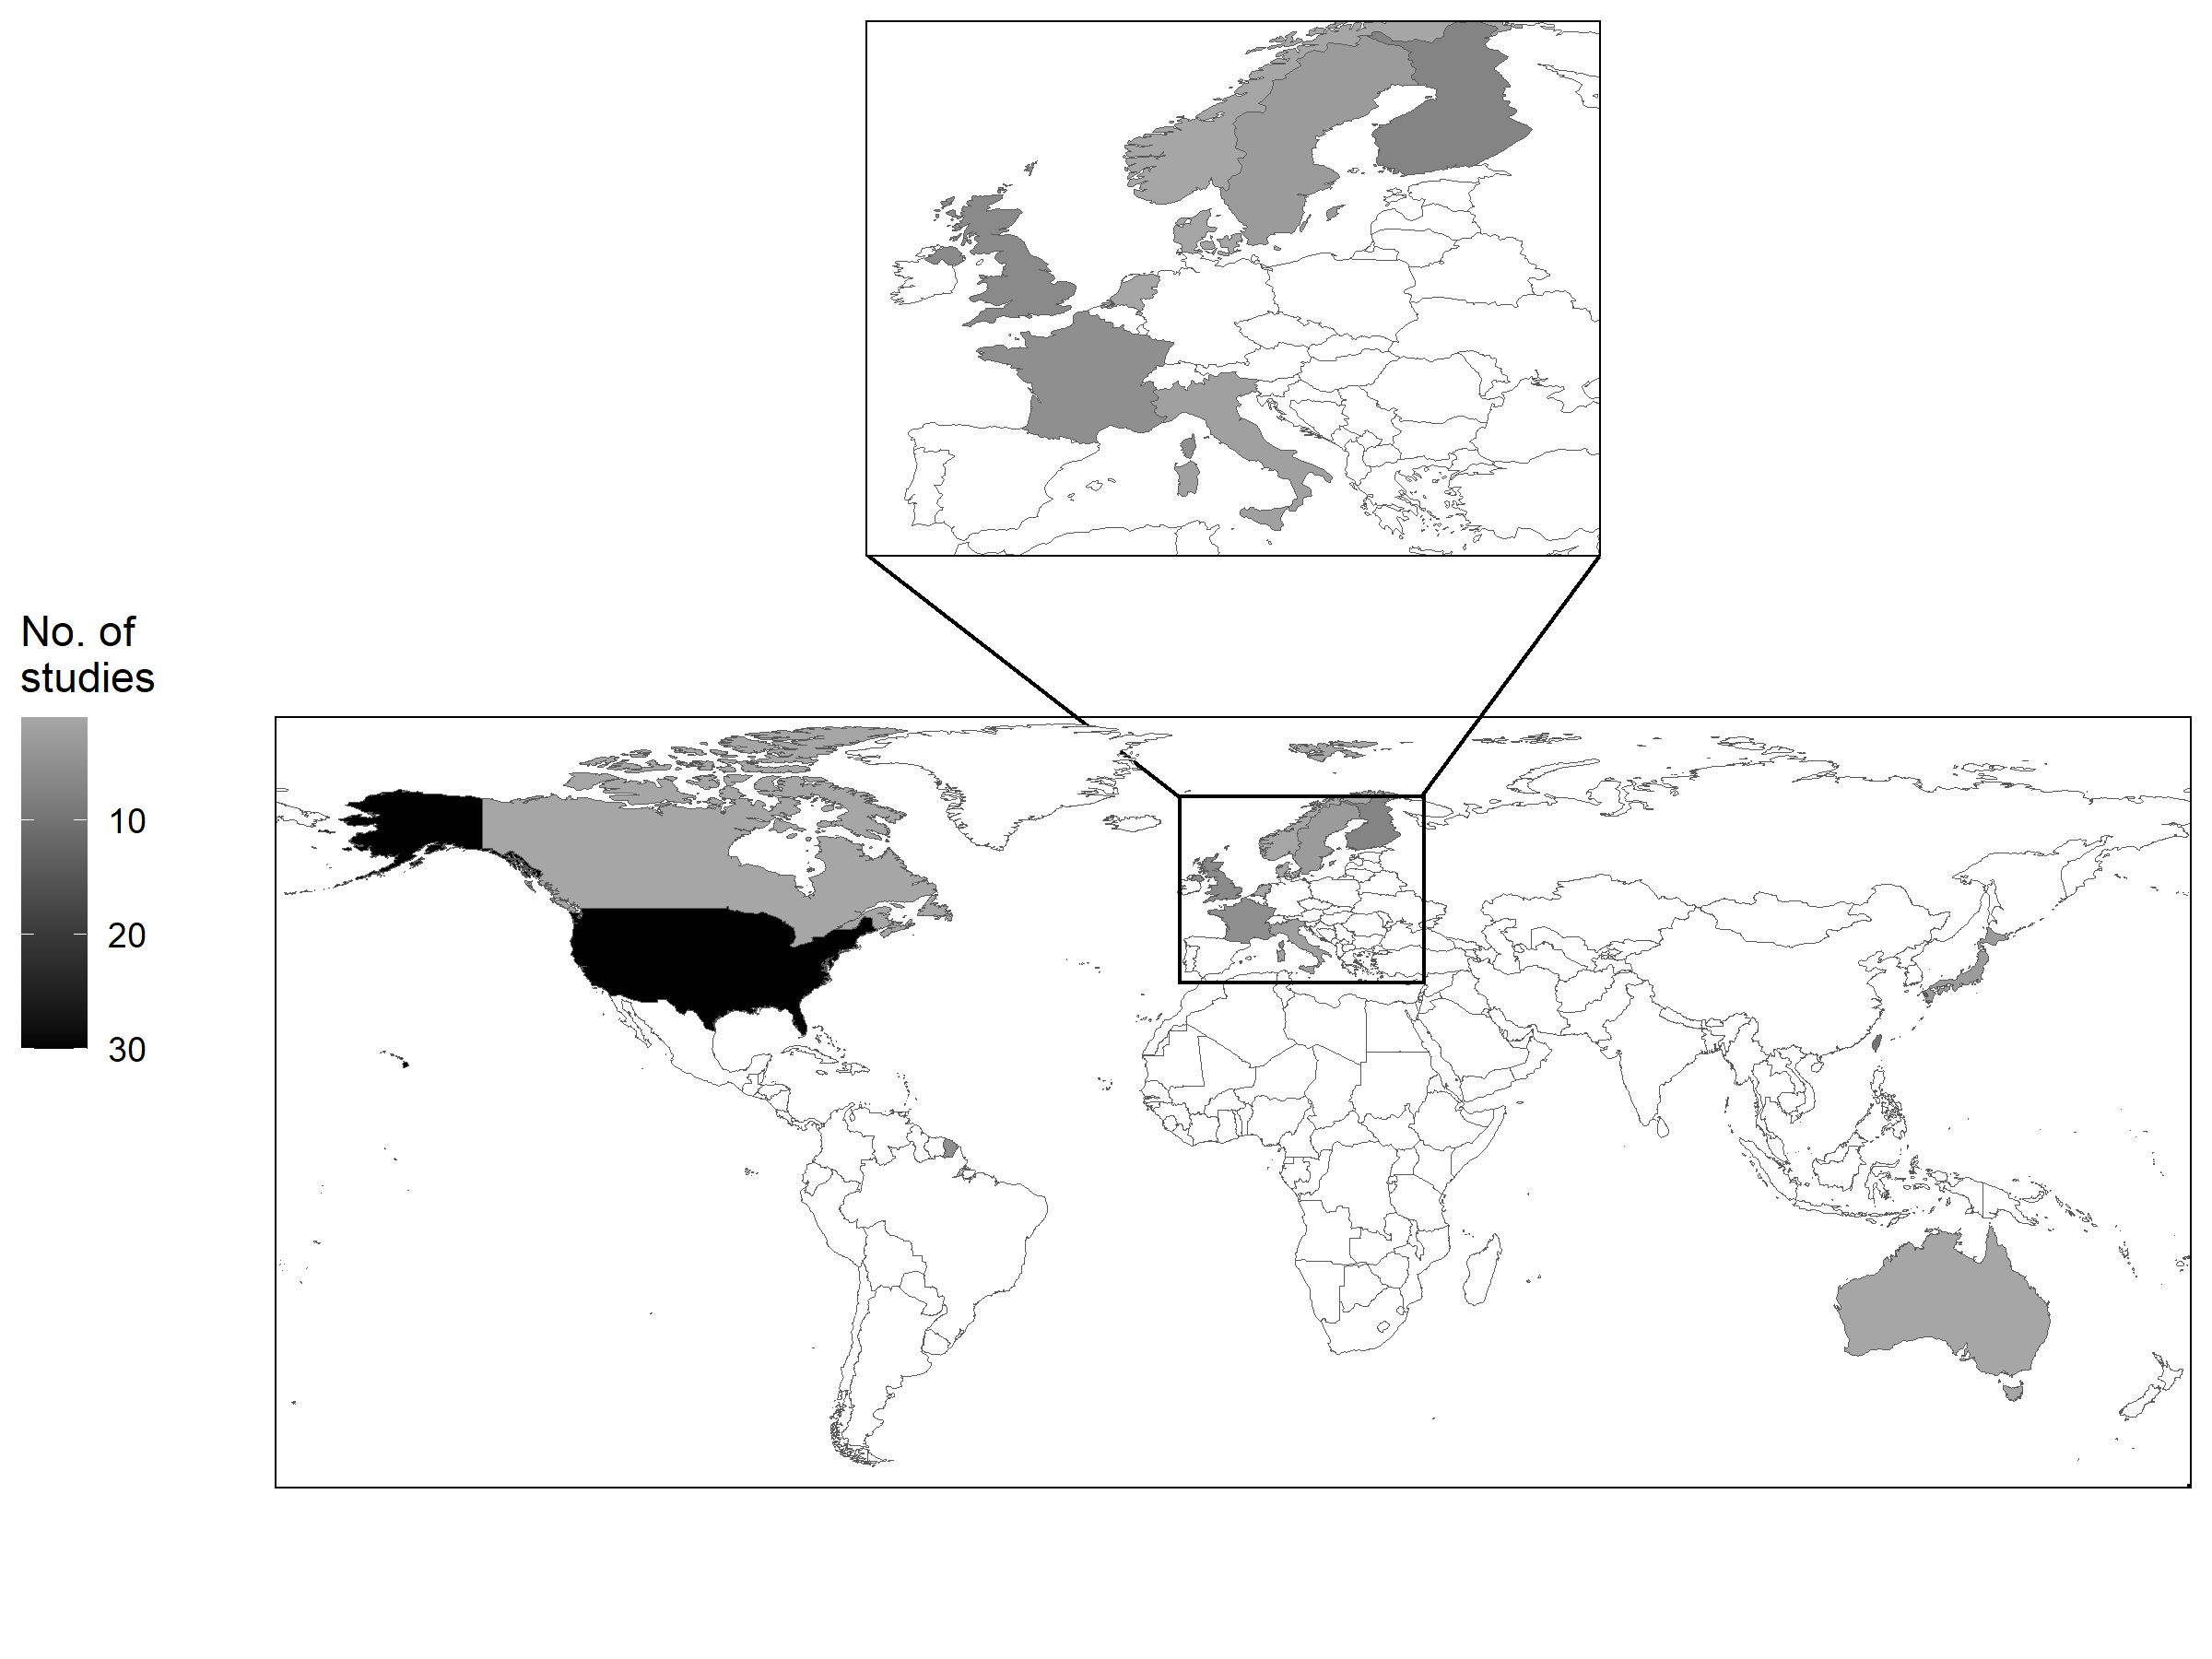
\includegraphics[width=1\linewidth]{figures/sys-rev/cohortLocations} \caption[Geographical distribution of study cohorts]{Geographical distribution of study cohorts}\label{fig:cohortLocations}
\end{figure}

~

Finally, there were several eligible studies reported as conference abstracts that did not present numerical results. These reports were included in the analysis to enable assessment of risk of bias due to missing evidence (see Section \ref{methods-rob-me}).

~

\hypertarget{risk-of-bias-res}{%
\subsection{Risk of bias}\label{risk-of-bias-res}}

As discussed above, the risk-of-bias assessments are presented alongside their corresponding numerical result. A more detailed discussion of the sources and directions of bias is presented in Chapter \ref{tri-heading}, and so this section presents a brief summary of the biases observed in each study design.

For the two randomised controlled trials, both were judged to be at low risk of bias. In contrast, many of the non-randomised studies of statin use were at serious risk of bias due poor controlling for confounding, immortal time bias, and missing outcome data (as noted above, a judgement of low risk of bias for a non-randomised study is rare). Similarly, non-randomised studies of exposures suffered from incomplete adjustment for potentially important confounders, and concerns over the selection of the reported result from among several analyses (e.g.~examination of lipids as a binary or continuous variable). Finally, bias was introduced into Mendelian randomisation studies via the potential for hoziontal pleiotropy and population stratification.\textsuperscript{\protect\hyperlink{ref-davies2018}{62}}

Following best practice, any result judged to be at critical risk of bias should be excluded from any quantitative analyses. Four observational studies were excluded on this basis, predominantly due to a lack of adjustment for any potentially important confounders (i.e.~the study reported unadjusted estimates).\textsuperscript{\protect\hyperlink{ref-kuo2015}{202},\protect\hyperlink{ref-mainousa.g.2005}{203},\protect\hyperlink{ref-notkola1998}{209}}

~

\hypertarget{sys-rev-res-Dementia}{%
\subsection{All-cause dementia}\label{sys-rev-res-Dementia}}

\hypertarget{statins}{%
\subsubsection{Statins}\label{statins}}

The two randomised controlled trials provided very weak evidence (OR: 1.07, 95\%CI: 0.70-1.66) of an effect on statin use on all-cause dementia risk (Figure \ref{fig:rctStatinDementiaFig}).





\begin{figure}[H]
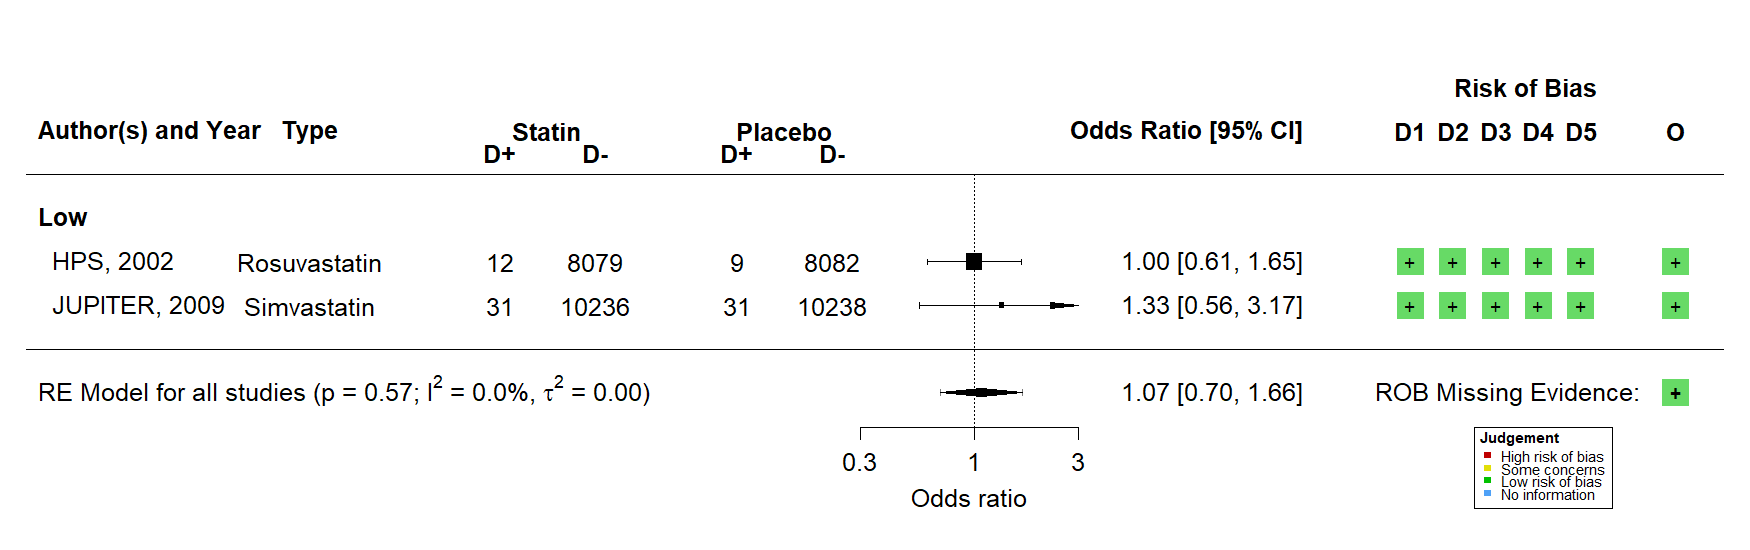
\includegraphics[width=1\linewidth]{figures/sys-rev/fp_rct_statins_Dementia} \caption[Random-effects meta-analysis of statins on all-cause dementia]{Random-effects meta-analysis of randomised controlled trials examining statin statins on all-cause dementia}\label{fig:rctStatinDementiaFig}
\end{figure}

~

In contrast, a meta-analysis of 15 prospective observational studies provided some evidence of a protective effect of statins use on all-cause dementia risk (HR: 0.77, 95\%CI: 0.65-0.90, Figure \ref{fig:obsStatinDementiaFig}).





\begin{figure}[H]
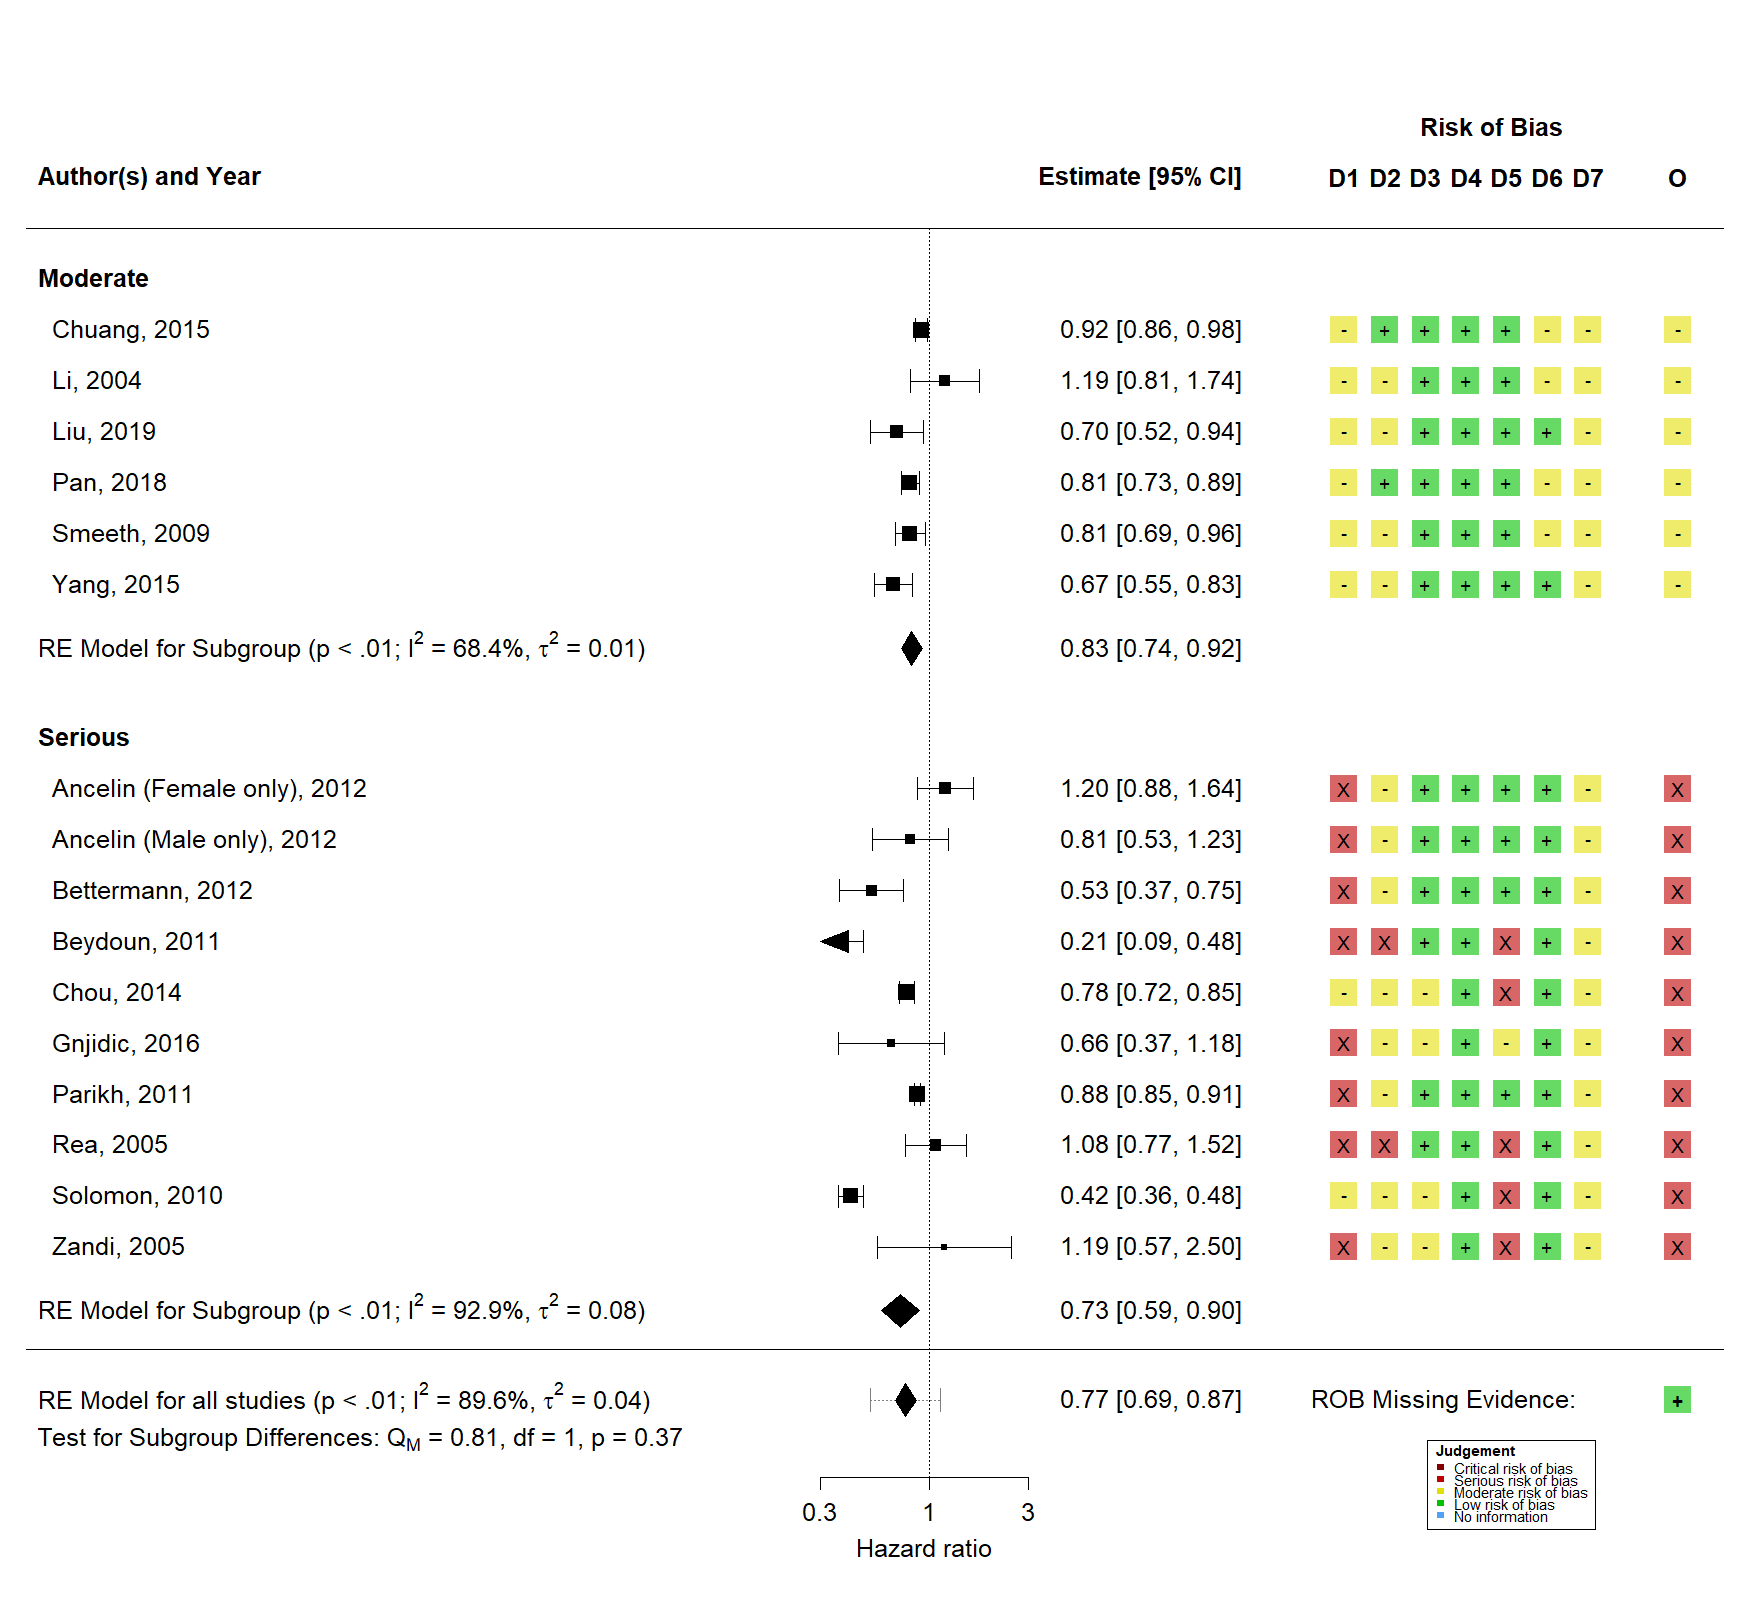
\includegraphics[width=1\linewidth]{figures/sys-rev/fp_obs_Statin-Ever_Dementia} \caption[Random-effects meta-analysis of statins on all-cause dementia]{Random-effects meta-analysis of non-randomised studies examining the effect of statin use on all-cause dementia}\label{fig:obsStatinDementiaFig}
\end{figure}

Finally, a single Mendelian randomisation analysis was identified examining the effect of lowered LDL-c levels on the risk of all-cause dementia via genetic inhibition of the 3-hydroxy-3-methylglutaryl-coenzyme A reductase (HMGCR), emulating statin treatment (see Section \ref{intro-statins} for more details of the statin mechanism of action). This analysis provided weak evidence for an effect (RR: 0.90, 95\%CI: 0.29-2.81).

~

\hypertarget{fibrates}{%
\subsubsection{Fibrates}\label{fibrates}}

Two studies examined the effect of fibrate use on all-cause dementia and found very weak evidence for an effect (HR: 0.90, 95\%CI: 0.75-1.07, Figure \ref{fig:obsFibrateDementiaFig}).





\begin{figure}[H]
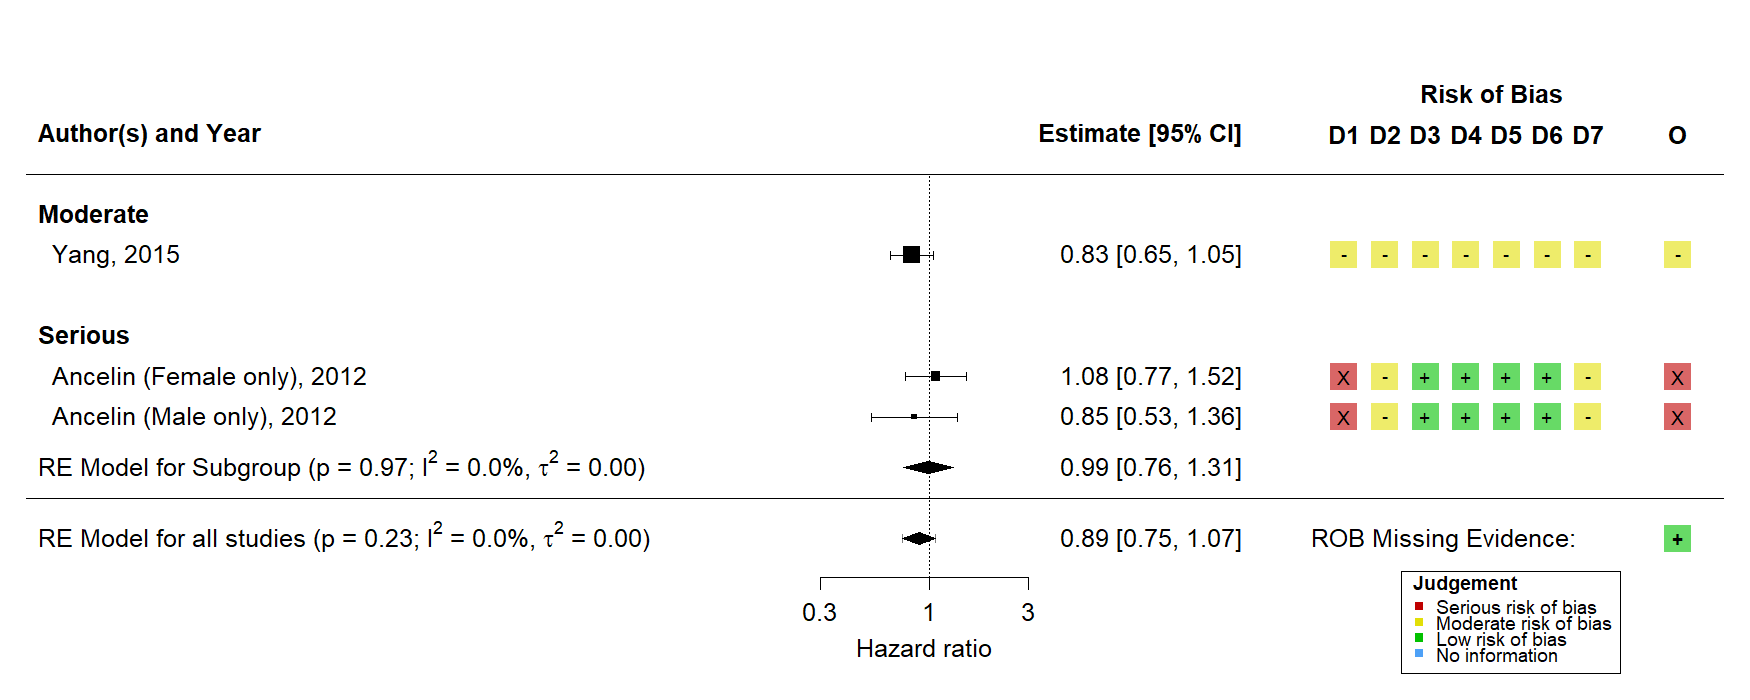
\includegraphics[width=1\linewidth]{figures/sys-rev/fp_obs_Fibrate_Dementia} \caption[Random-effects meta-analysis of statins on all-cause dementia]{Random-effects meta-analysis of non-randomised studies examining the effect of fibrate use on all-cause dementia}\label{fig:obsFibrateDementiaFig}
\end{figure}

\hypertarget{lipids}{%
\subsubsection{Lipids}\label{lipids}}

Across all outcomes, lipid levels were categorised in a number of ways. The most common categorisation was hypercholesterolemia at baseline, defined most frequently as a total cholesterol measurement of greater than 6.5 mmol/L.

Eleven studies reported on the association of hypercholesterolemia with all-cause dementia and provided weak evidence for an effect (HR: 1.11, 95\%CI: 0.99-1.24, Figure \ref{fig:obsHyperDementia}).





\begin{figure}[H]
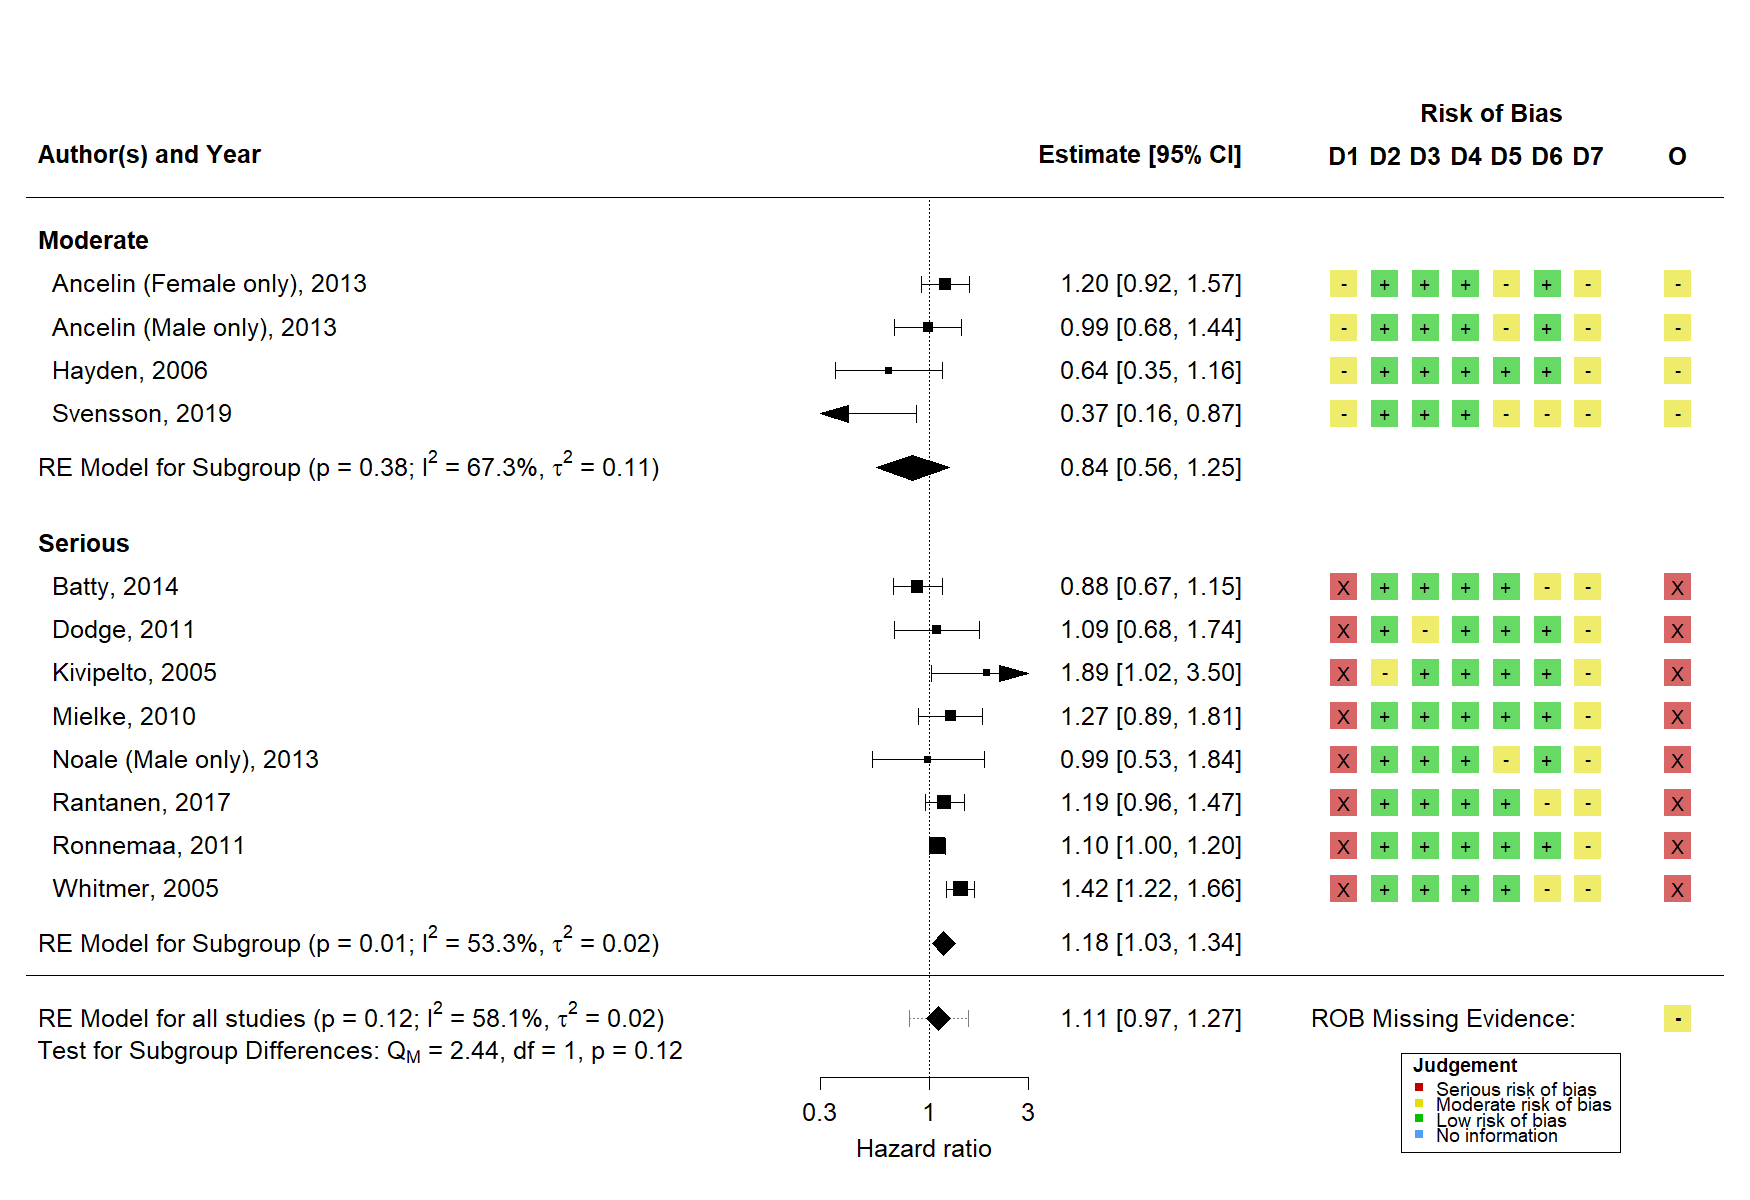
\includegraphics[width=1\linewidth]{figures/sys-rev/fp_obs_hyperchol_Dementia} \caption[Meta-analysis of hypercholesterolemia on all-cause dementia]{Random-effects meta-analysis of non-randomised studies examining the effect of hypercholesterolemia on all-cause dementia}\label{fig:obsHyperDementia}
\end{figure}

Several studies analysed individual lipid fractions by estimating the risk of dementia per 1 standard deviation increase in that fraction (Figure \ref{fig:lipidFractionsDementia}). Very weak evidence for an effect on all-cause dementia was found for total cholesterol (N = 5; HR: 0.97, 95\%CI: 0.87-1.07), LDL-c (N = 2; HR: 0.96, 95\%CI: 0.86-1.08), HDL-c (N = 4; HR: 1.04, 95\%CI: 0.96-1.13) and triglycerides (N = 3; HR: 0.90, 95\%CI: 0.75-1.08).





\begin{figure}[H]
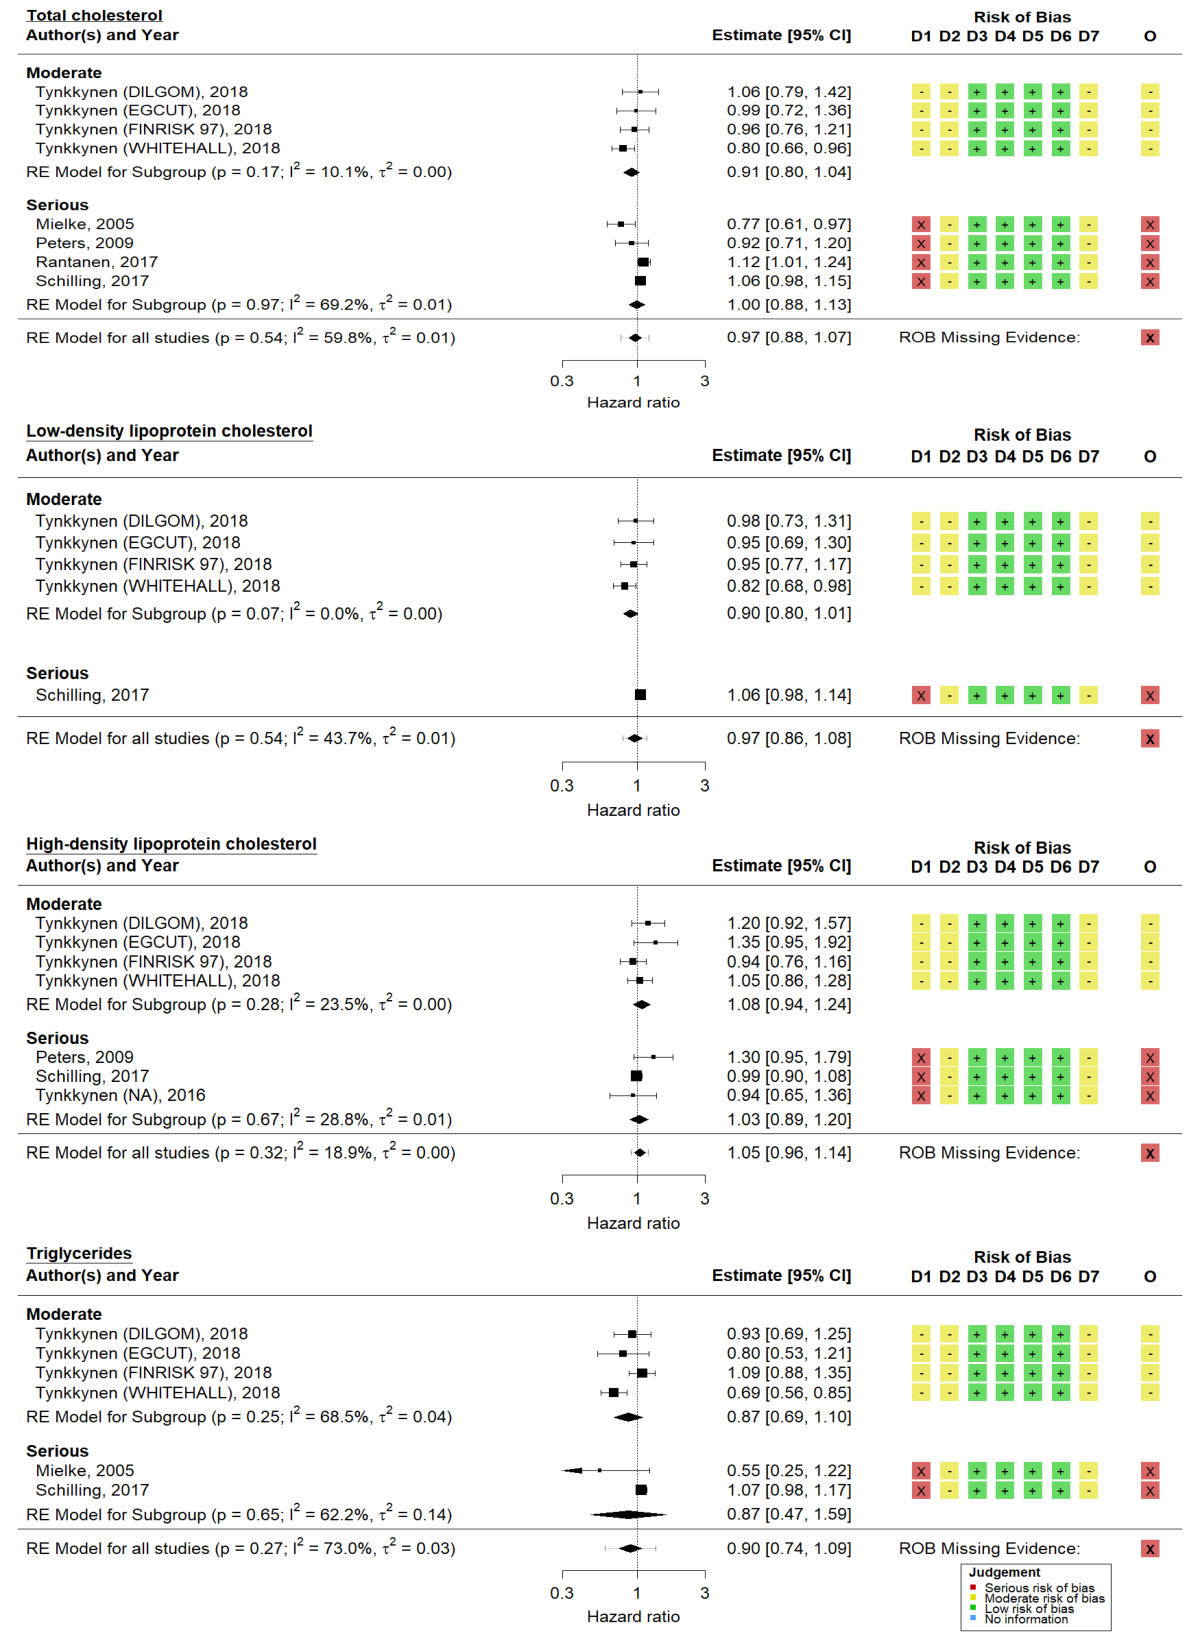
\includegraphics[width=1\linewidth]{figures/sys-rev/fp_lipids_composite_Dementia} \caption[Random-effects meta-analysis of four lipid fractions on all-cause dementia]{Random-effects meta-analysis of four lipid fractions (total cholesteol, HDL, LDL, and triglycerides) on all-cause dementia risk, standardised per 1-SD increase in the lipid fraction.}\label{fig:lipidFractionsDementia}
\end{figure}

Finally, there were no identified Mendelian randomisation analysis examining the effect of lower lipid levels, as determined by any genetic instrument, on all-cause dementia risk.

~

\hypertarget{sys-rev-res-AD}{%
\subsection{Alzheimer's disease}\label{sys-rev-res-AD}}

\hypertarget{statins-1}{%
\subsubsection{Statins}\label{statins-1}}

There were no randomised trials of the use of statins or any other lipid regulating agents on Alzheimer's disease, though several observational studies reported on this outcome and provided evidence for a protective effect (N = 11; HR: 0.83, 95\%CI: 0.69-1.00; Figure \ref{fig:obsStatinADFig}).





\begin{figure}[H]
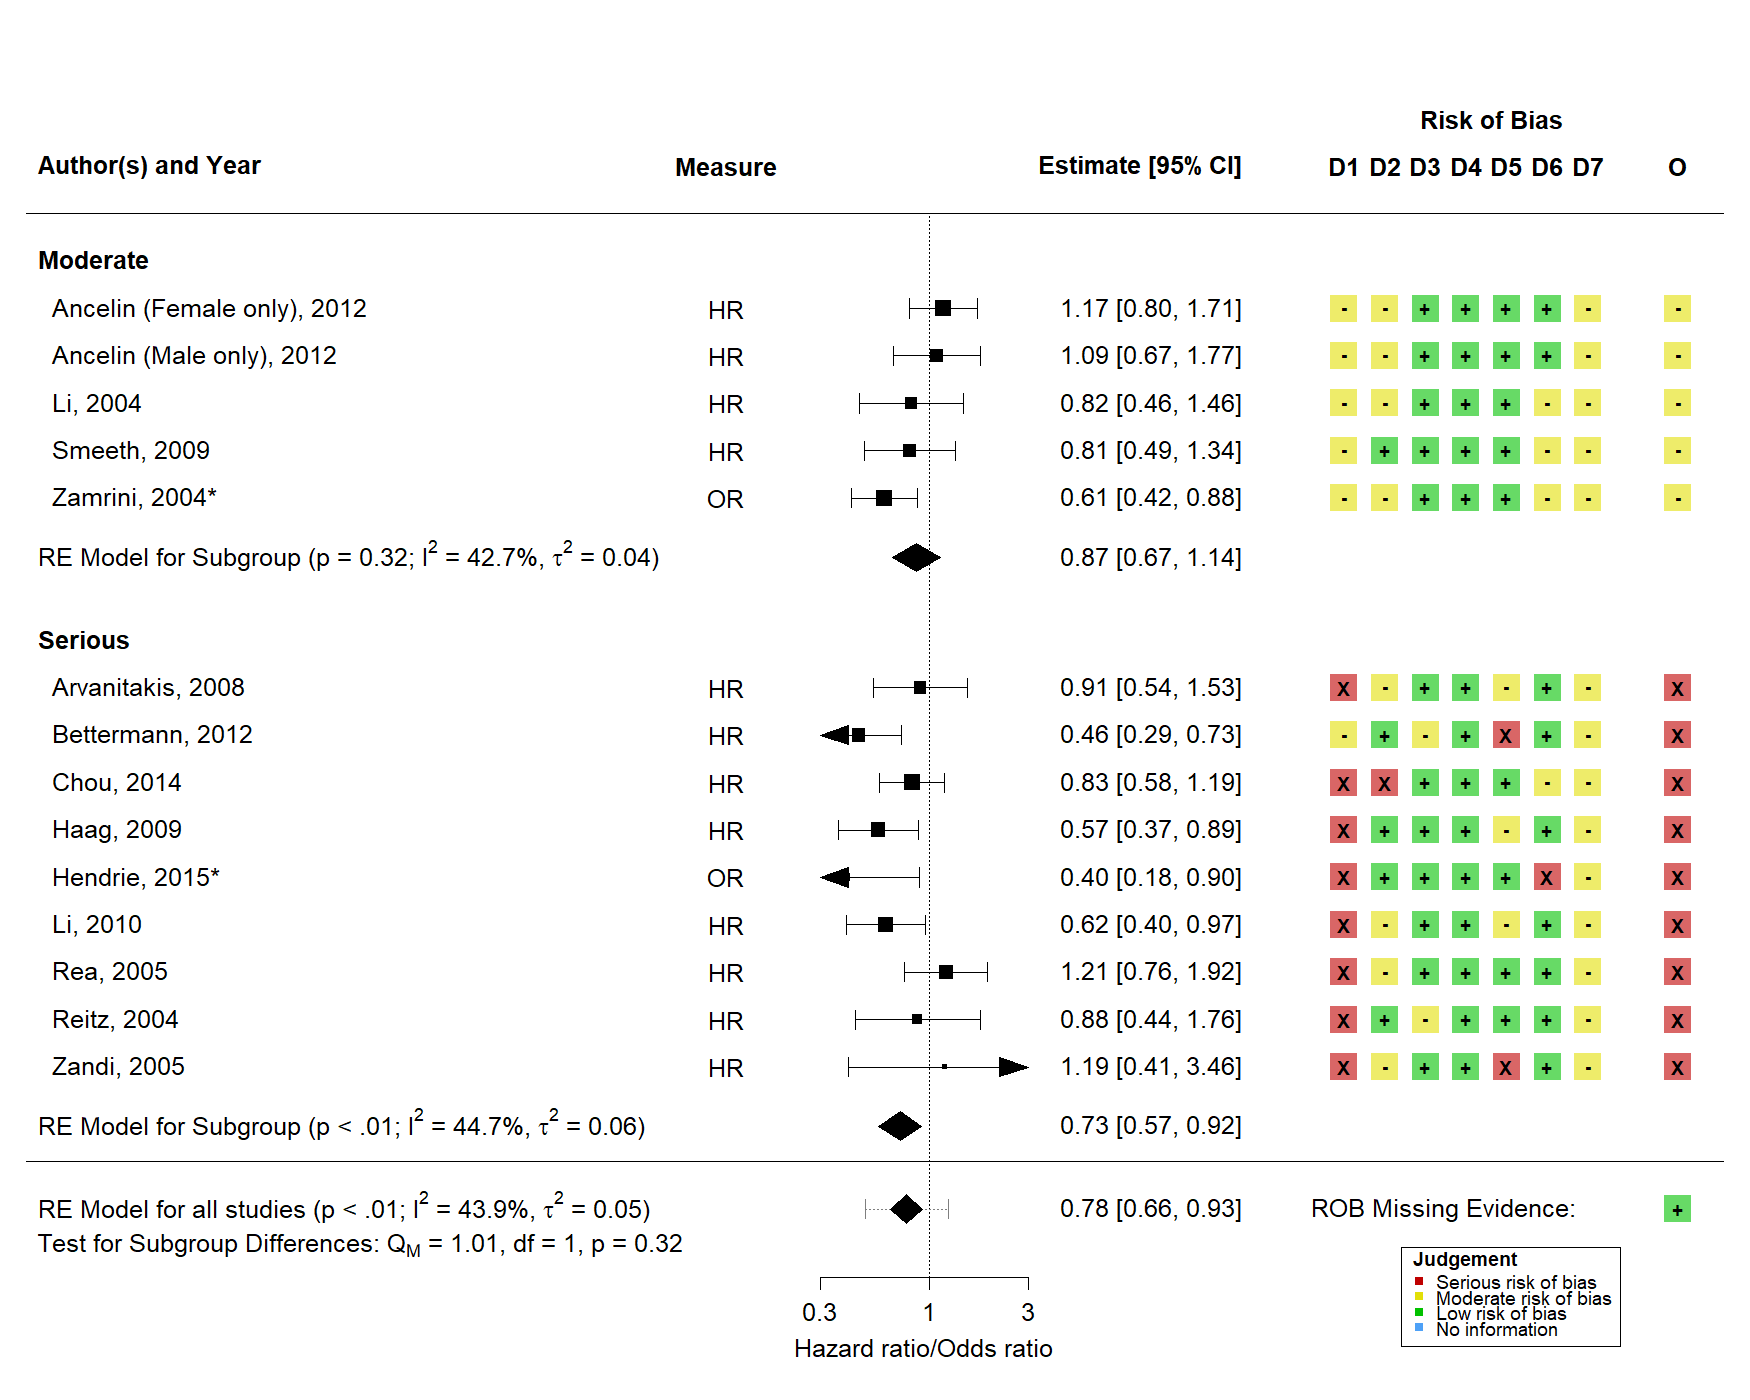
\includegraphics[width=1\linewidth]{figures/sys-rev/fp_obs_Statin-Ever_AD} \caption[Random-effects meta-analysis of statins on Alzheimer's disease]{Random-effects meta-analysis of non-randomised studies examining the effect of statin use on Alzheimer's disease}\label{fig:obsStatinADFig}
\end{figure}

Two Mendelian randomisation studies looked at specifically as a result of HMGCR inhibition, mediated by SNPs in the gene (rs172338484 and rs12916).\textsuperscript{\protect\hyperlink{ref-benn2017b}{191},\protect\hyperlink{ref-so2017}{232}} The first used a one sample approach (SNP-exposure and SNP-outcome associations are estimated using the same dataset) in a large Copenhagen-based cohort, while the second made use of summary level data obtained from the Global Lipids Genetic Consortium (SNP-exposure) and the International Genomics of Alzheimer's Project (SNP-outcome). Meta-analysis of these estimates provided weak evidence of an effect (RR: 0.76, 95\%CI: 0.51-1.14, Figure \ref{fig:mrStatinADFig}).





\begin{figure}[H]
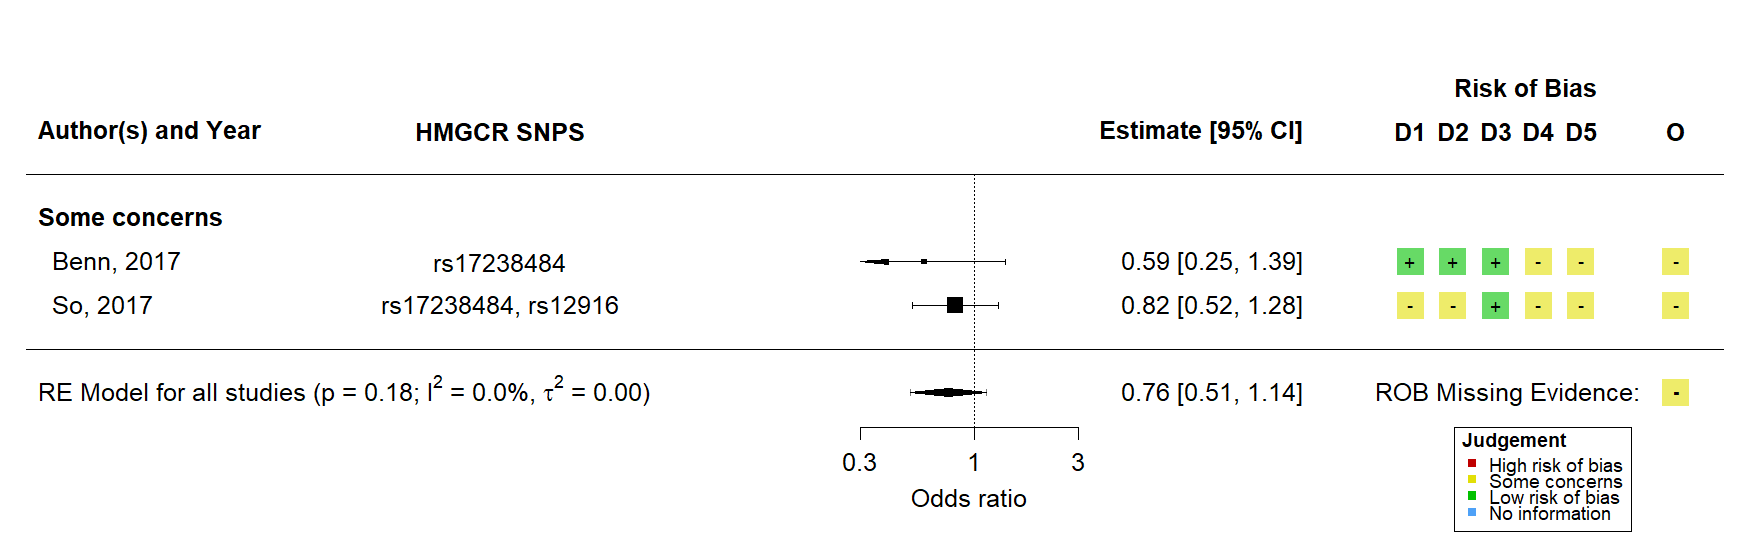
\includegraphics[width=1\linewidth]{figures/sys-rev/fp_MR_HMGCR_AD} \caption[Random-effects meta-analysis of genetically lowered LDL-c via HMGCR inhibition on Alzheimer's disease]{Random-effects meta-analysis of genetically lowered LDL-c via HMGCR inhibition on Alzheimer's disease}\label{fig:mrStatinADFig}
\end{figure}

~

\hypertarget{lipids-1}{%
\subsubsection{Lipids}\label{lipids-1}}

9 studies reported on the association of hypercholesterolemia with all-cause dementia and provided weak evidence for an effect (HR: 0.99, 95\%CI: 0.78-1.25, Figure \ref{fig:obsHyperAD})





\begin{figure}[H]
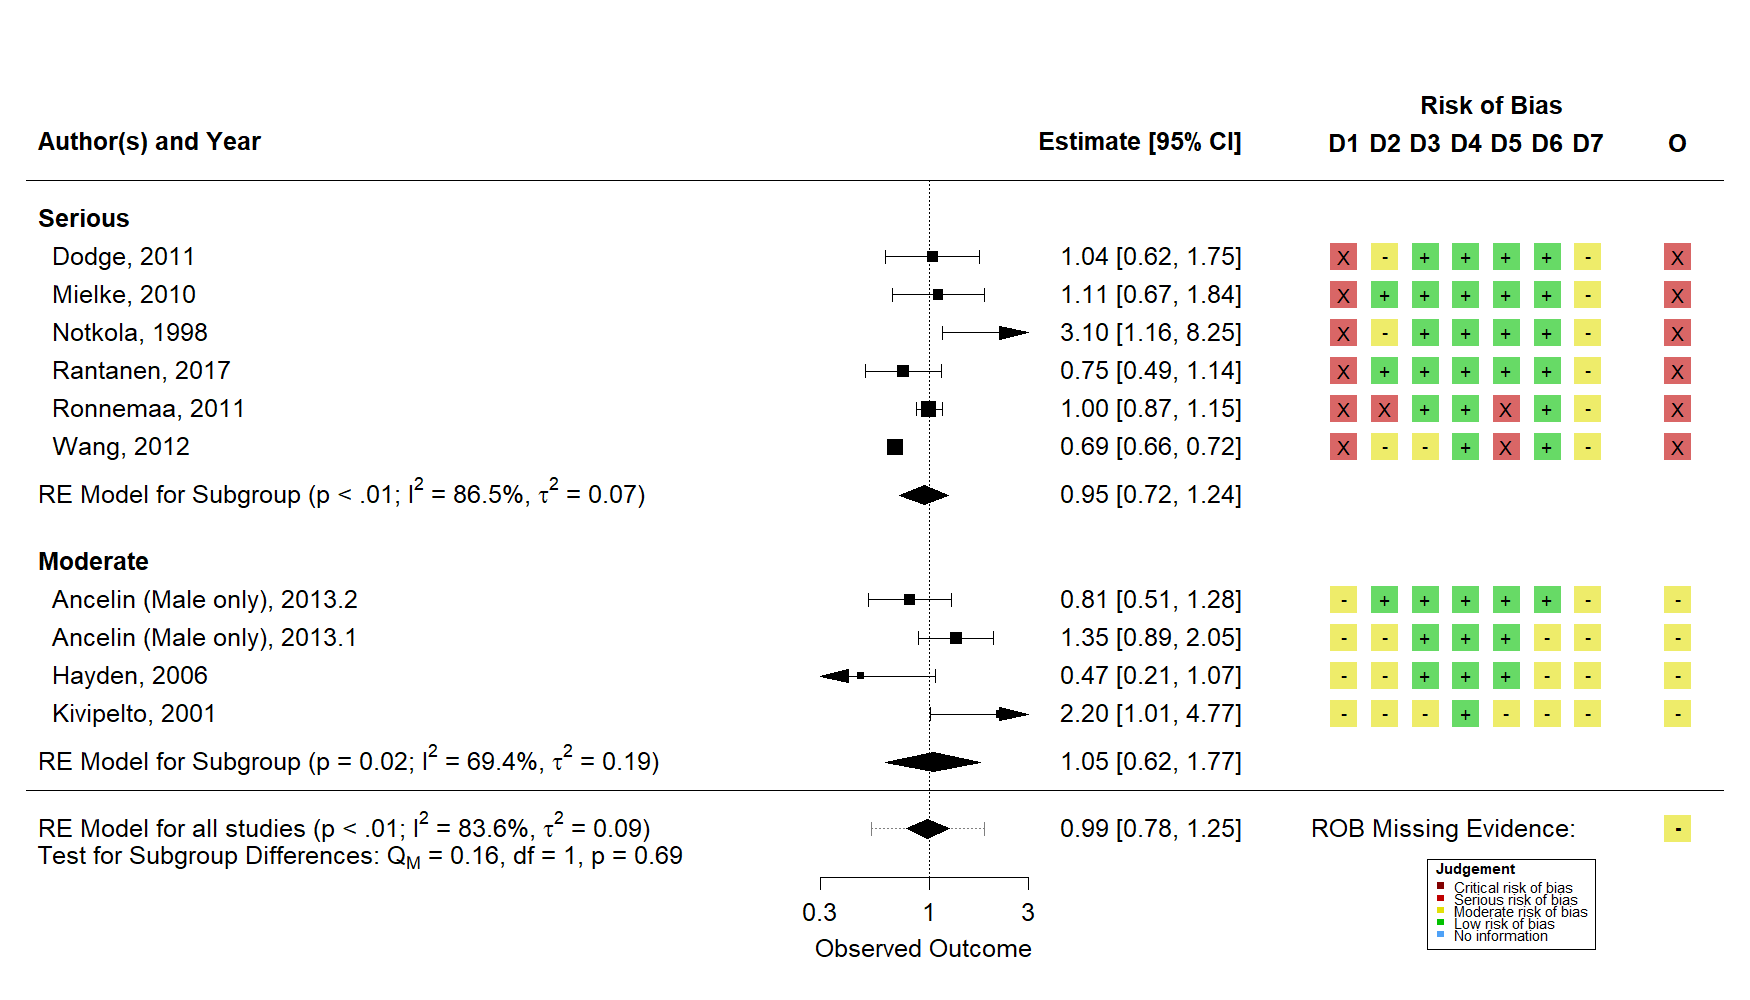
\includegraphics[width=1\linewidth]{figures/sys-rev/fp_obs_hyperchol_AD} \caption[Meta-analysis of hypercholesterolemia on Alzheimer's disease]{Random-effects meta-analysis of non-randomised studies examining the effect of hypercholesterolemia on Alzheimer's disease}\label{fig:obsHyperAD}
\end{figure}

Similarly to all-cause dementia, several studies analysed individual lipid fractions by estimating the risk of dementia per 1 standard deviation increase in that fraction (Figure \ref{fig:lipidFractionsAD}). Very weak evidence for an effect on all-cause dementia was found for total cholesterol (N = 5; HR: 1.00, 95\%CI: 0.93-1.07), LDL-c (N = 3; HR: 1.03, 95\%CI: 0.91-1.16), HDL-c (N = 4; HR: 0.99, 95\%CI: 0.91-1.07) or triglycerides (N = 3; HR: 0.99, 95\%CI: 0.83-1.19).





\begin{figure}[H]
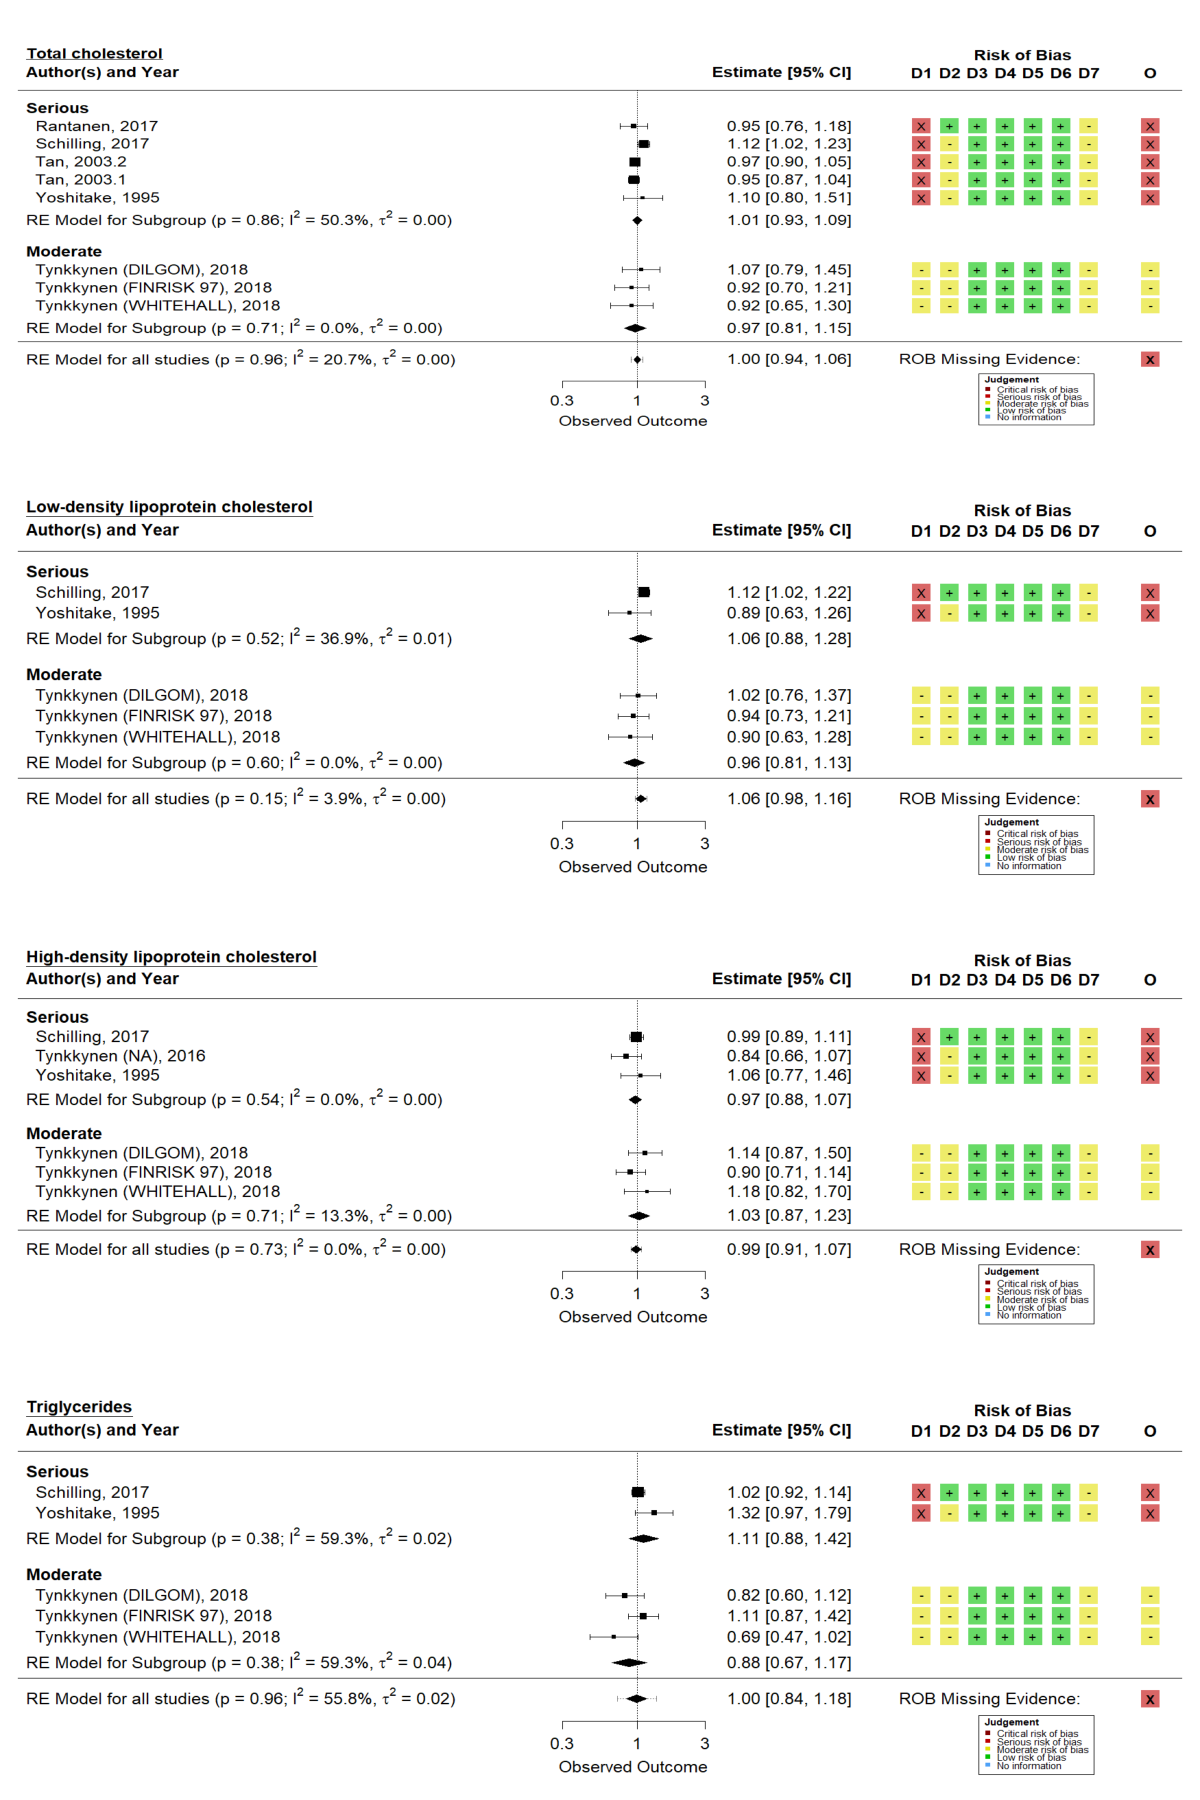
\includegraphics[width=1\linewidth]{figures/sys-rev/fp_lipids_composite_AD} \caption[Random-effects meta-analysis of four lipid fractions on Alzheimer's disease]{Random-effects meta-analysis of four lipid fractions (total cholesteol, HDL, LDL, and triglycerides) on Alzheimer's disease risk, standardised per 1-SD increase in the lipid fraction.}\label{fig:lipidFractionsAD}
\end{figure}

Finally, there were several identified Mendelian randomisation studies examining the effect of genetically lowered LDL-c on Alzheimer's disease risk (Figure \ref{fig:mrDuplication}). However, all of these studies used a two-sample approach, making use of summary statistics from the GLGC and IGAP consortia. Due to this overlap, which would result in a falsely precise estimate caused by multiple counting of the same participants, no meta-analysis of these studies was performed. However, across all analysis, using varying number of SNPS, no evidence for an effect was observed (Figure \ref{fig:mrDuplication}).





\begin{figure}[H]

{\centering 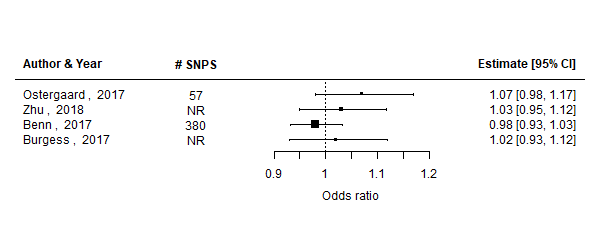
\includegraphics[width=0.8\linewidth]{figures/sys-rev/mrDuplication} 

}

\caption[Summary of duplication across two sample Mendelian randomisation studies]{Summary of duplication across Mendelian randomisation studies which used summary statistics from the Global Lipid Genetics Consortium (GLGC) and the International Genomics of Alzheimer's Project (IGAP). Note that the Alzheimer's Disease Genetics Consortium (ADGC) is a sub-cohort within IGAP.}\label{fig:mrDuplication}
\end{figure}

~

\hypertarget{sys-rev-res-VaD}{%
\subsection{Vascular dementia}\label{sys-rev-res-VaD}}

\hypertarget{statins-2}{%
\subsubsection{Statins}\label{statins-2}}

As noted in Section \ref{sys-rev-characteristics} above, there was substantially less literature available on the association of my risk factors of interest and vascular dementia. There were no available randomised trials for this outcome. Three prospective cohort studies examined statin use and vascular dementia, though meta-analysis of these studies provided very weak evidence for an effect (N = 3; HR: 1.02, 95\%CI: 0.77-1.36; Figure \ref{fig:obsStatinVaDFig}).





\begin{figure}[H]
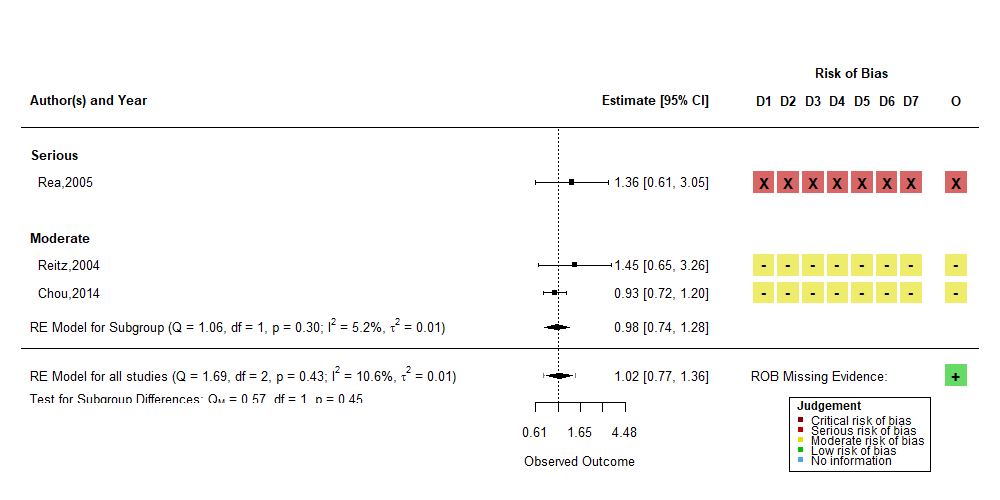
\includegraphics[width=1\linewidth]{figures/sys-rev/fp_obs_Statin-Ever_VaD} \caption[(ref:obsStatinDVaD-scap)]{Random-effects meta-analysis of non-randomised studies examining effect of statin use on vascular dementia}\label{fig:obsStatinVaDFig}
\end{figure}

A single Mendelian randomisation analysis was identified that examining the effect of genetically lowered LDL-c levels via HMGCR inhibition on the risk of vascular dementia, which provided weak evidence for an effect (RR: 0.44, 95\%CI: 0.21-0.91).

~

\hypertarget{lipids-2}{%
\subsubsection{Lipids}\label{lipids-2}}

Three studies reported on the association of hypercholesterolemia with vascular dementia and provided weak evidence for an effect (HR: 1.20, 95\%CI: 1.00-1.44, Figure \ref{fig:obsHyperVaD})





\begin{figure}[H]
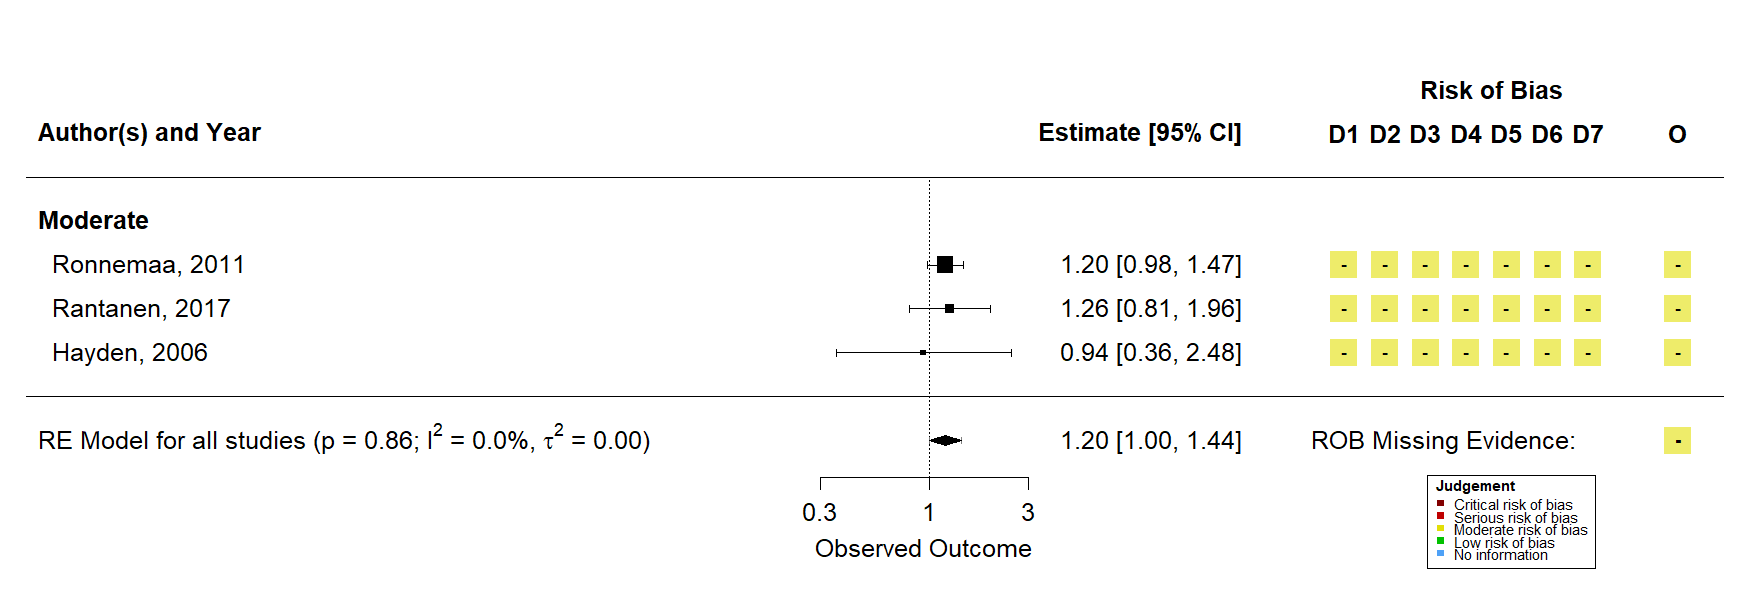
\includegraphics[width=1\linewidth]{figures/sys-rev/fp_obs_hyperchol_VaD} \caption[Meta-analysis of hypercholesterolemia on vascular dementia]{Random-effects meta-analysis of non-randomised studies examining the effect of hypercholesterolemia on vascular dementia}\label{fig:obsHyperVaD}
\end{figure}

Few studies investigated the effect of individual lipid fractions. Only for total cholesterol was there greater than one result reported (Figure \ref{fig:lipidFractionsVaD}), and a meta-analysis of these found very weak evidence for an effect (N = 2; HR: 1.05, 95\%CI: 0.79-1.41). A single study provided evidence on the other three fractions,\textsuperscript{\protect\hyperlink{ref-yoshitake1995}{225}} and similar found minimal evidence of an effect LDL-c (N = 1; HR: 1.12, 95\%CI: 0.83-1.51), HDL-c (N = 1; HR: 0.83, 95\%CI: 0.60-1.14) or triglycerides (N = 1; HR: 1.00, 95\%CI: 0.75-1.34).





\begin{figure}[H]
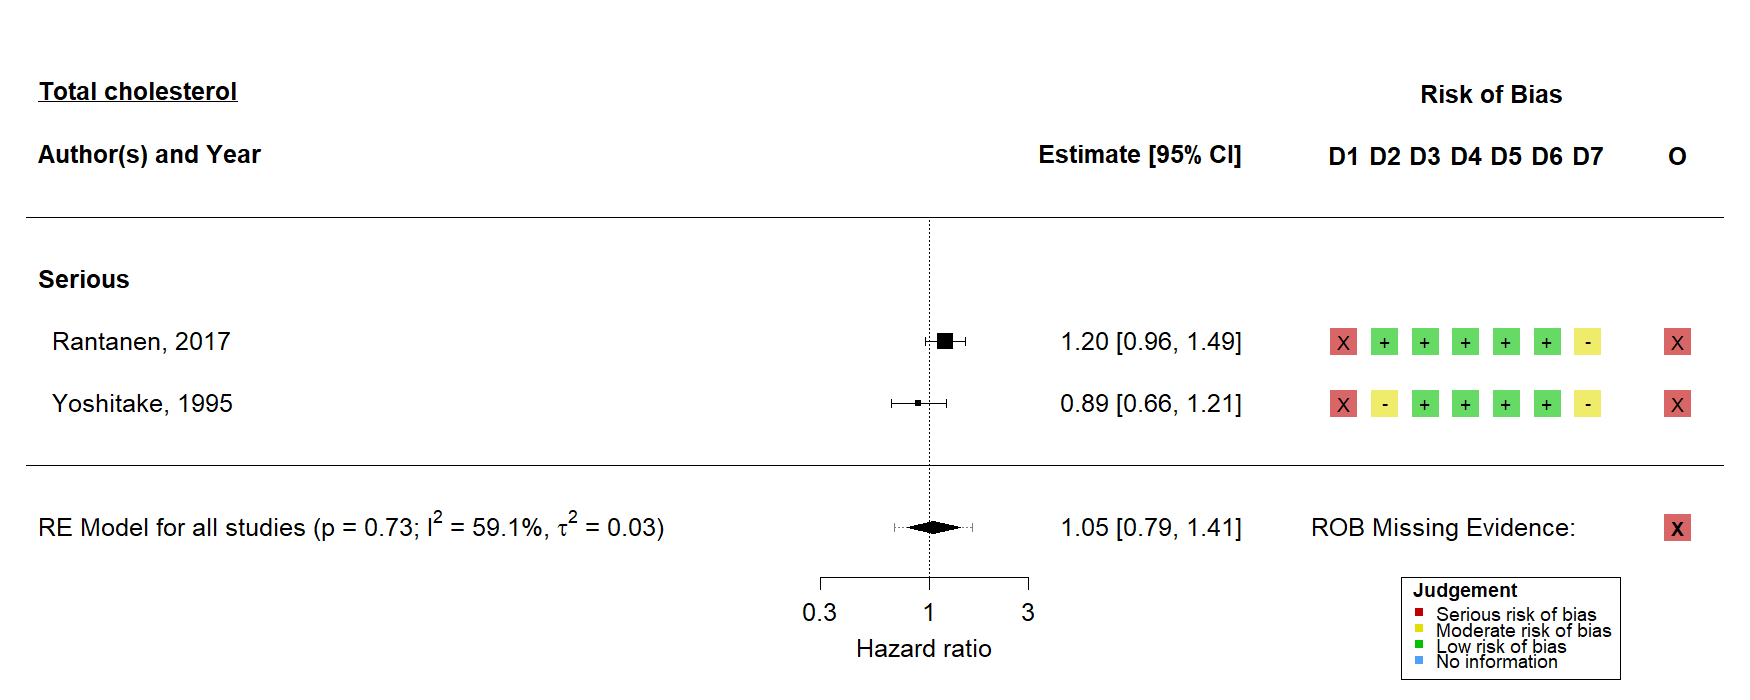
\includegraphics[width=1\linewidth]{figures/sys-rev/fp_obs_VaD_TC_} \caption[Random-effects meta-analysis of four lipid fractions on Alzheimer's disease]{Random-effects meta-analysis of four lipid fractions (total cholesteol, HDL, LDL, and triglycerides) on Alzheimer's disease risk, standardised per 1-SD increase in the lipid fraction.}\label{fig:lipidFractionsVaD}
\end{figure}

Finally, there were no identified Mendelian randomisation analysis examining the effect of genetically determined lipid levels on vascular dementia risk.

~

\hypertarget{dose-response-results}{%
\subsection{Dose response meta-analysis of lipid levels}\label{dose-response-results}}

There were 13 studies that were eligible for dose-response meta-analysis as they provide several categories of lipid exposure. However, following data extract, five were excluded as they did not reported the relevant information needed (most commonly, the cut-off measures for each category).

Across the remaining eight studies, a sufficient number of studies (n \(\geqslant\) 3) were identified only for the total cholesterol-Alzheimer's, LDL-Alzheimer's, and total cholesterol-dementia strata. This analysis provided very weak evidence for a non-linear effect of lipid levels on dementia outcomes, and Figure \ref{fig:lipidsDoseResponse} illustrates this for the total cholesterol-Alzheimer's strata. Similar figures for the other analysed lipid-outcome strata are presented in Appendix \ref{hold}.





\begin{figure}[H]

{\centering 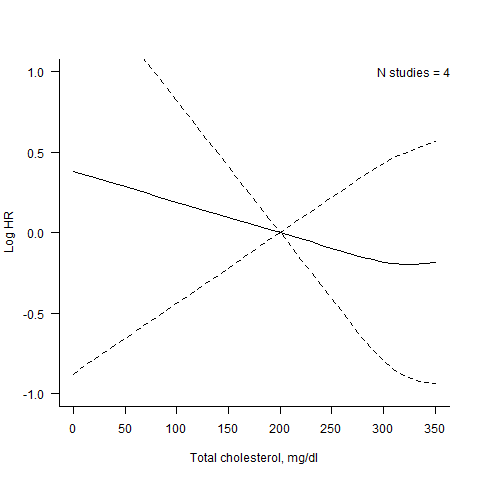
\includegraphics[width=0.7\linewidth]{figures/sys-rev/dr_AD_TC} 

}

\caption[Dose-response meta-analysis of total cholesterol]{Dose-response meta-analysis of total cholesterol on Alzheimer's disease}\label{fig:lipidsDoseResponse}
\end{figure}

~

\hypertarget{additional-analyses-1}{%
\subsection{Additional analyses}\label{additional-analyses-1}}

Investigation of potential sources of heterogeneity was complicated by two factors. In the first instance, few meta-analysis included more than 10 results, the recommended minimum required for meta-regression. Secondly, poor reporting of summary statistics including education level and baseline cognitive ability precluded the use of several results in a meta-regression analysis.

Age and sex were assessed as potential causes of heterogeneity in the meta-analyses of statin use and hypercholesterolemia on all cause dementia and Alzheimer's disease, but I found very weak evidence for variation in the observed effect estimates due to these factors.

Similarly, assessment of small-study effects, for which publication bias could be one potential reason, was hindered by the relatively small number of results included in a given meta-analysis. However, all analyses assessed provided weak evidence of small-study effects.

{[}\emph{Note: Julian, is this sufficient or should I report statistics for each? Additionally, are there any other sensitivity analyses I should be presenting here?}{]}

~

~

\hypertarget{missing-evidence}{%
\subsection{Missing evidence}\label{missing-evidence}}

The risk of bias due to missing evidence in each synthesis is shown beside the overall summary diamond in each forest plot presented above. For randomised controlled trials and non-randomised studies of interventions, the risk of bias due to missing evidence was assessed to be minimal. However, there was substantial evidence that results were selectively reported in studies examining the effect of lipid fractions on dementia outcomes (Figures \ref{fig:lipidFractionsDementia}, \ref{fig:lipidFractionsAD} and \ref{fig:lipidFractionsVaD}.

~

\hypertarget{sys-rev-including-preprints-res}{%
\subsection{Added evidential value of including preprints}\label{sys-rev-including-preprints-res}}

As show in Figure \ref{fig:prisma-flow-fig}, the number of hits returned by the preprint searching was not substantial (bioRxiv = 256, medRxiv = 0). From these hits, three preprinted reports of eligible studies were included in the review, of which two described unique studies not captured by the main search.\textsuperscript{\protect\hyperlink{ref-so2017}{232},\protect\hyperlink{ref-andrews2019}{235}}

Including preprints did provide useful additional evidential value in a number of meta-analysis. To demonstrate this, the effect of HMGCR SNPS on Alzheimer's disease (Figure \ref{fig:mrStatinADFig}) in Mendelian randomisation studies was re-analysed using a fixed-effect model. Examination of the weight assigned to each result in the analysis illustrates that a large proportion (78\%) of the weight is given to the preprinted result.

Investigation of the publication status of the two preprints reporting studies not also identified by the main search after a two-year lag found that one had been subsequently published in late 2019.\textsuperscript{\protect\hyperlink{ref-andrews2021}{227},\protect\hyperlink{ref-andrews2019}{235}} The final preprint has not yet been published.\textsuperscript{\protect\hyperlink{ref-so2017}{232}}

~

\hypertarget{discussion-1}{%
\section{Discussion}\label{discussion-1}}

This review has presented a summary of the available evidence on the association between lipids, and treatments that modify lipids such as statins, and the subsequent risk of dementia. This discussion seeks to to summarise the key findings in terms of literature sources and results as reported. A detailed comparison across the evidence sources, exposure measures and sources of bias reported here is presented as part of the triangulation exercise in Chapter \ref{tri-heading}.

~

\hypertarget{summary-of-findings}{%
\subsection{Summary of findings}\label{summary-of-findings}}

There was some evidence of protective effect of statins on all-cause and Alzheimer's disease dementia when looking at solely at observational studies. This finding was not supported by evidence from the two available RCTs, or by studies that emulated statin treatment using a genetic proxy, suggesting that these findings may be a result of heterogeneity in exposure (e.g.~mid-life in studies of lipids with late-life lipid reduction in RCTs) or alternatively due to biases within the non-randomised studies.

The majority of studies were non-randomised studies of lipids, or treatments that affect lipid levels such as statins. This distribution of evidence between analytical designs is to be expected. Randomised controlled trials of dementia are particularly challenging, as the long follow-up made necessary by the long latent period of the condition, makes trials logistically challenging and financial expensive. Similarly, Mendelian randomisation is a comparatively new study design (as illustrated in Figure \ref{fig:typeByYear}), which appears in the literature in recent years, driven by the availability of summary genome wide association studies (GWAS) that form the basis of the two-sample Mendelian randomisation approach.

~





\begin{figure}[H]
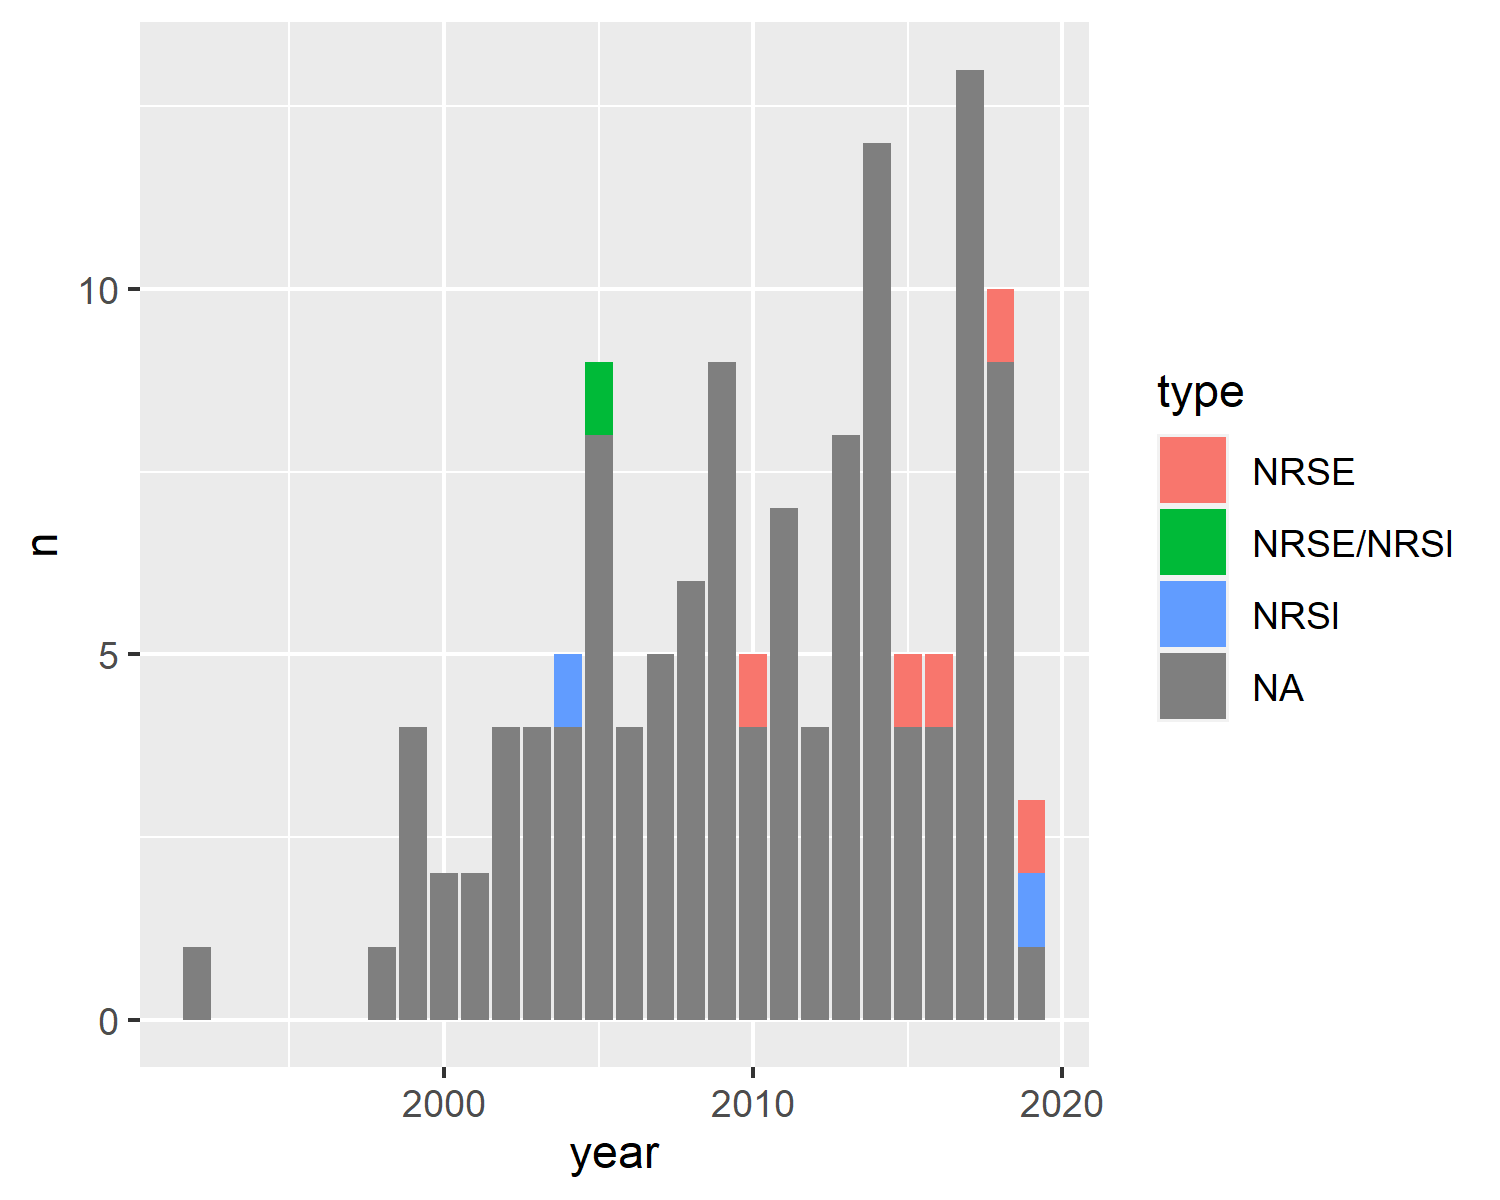
\includegraphics[width=1\linewidth]{figures/sys-rev/type_by_year} \caption[Study designs by year of publication]{Included study designs by year of publication}\label{fig:typeByYear}
\end{figure}

~

A common theme was an absence of studies examining vascular dementia as an outcome, most noticeable when comparing the evidence base for statins in dementia/Alzheimer's (Figures \ref{fig:obsStatinDementiaFig} \& \ref{fig:obsStatinADFig}) with that available for vascular dementia (Figure \ref{fig:obsStatinVaDFig}). This is particularly interesting given that lipids and statins are strongly related to the prevention of vascular disease. A potential explanation for this observation may be publication bias or the ``file-drawer effect'',\textsuperscript{\protect\hyperlink{ref-rosenthal1979}{76}} though there was very weak evidence of a small-study effects for this outcome (of which publication bias is a potential cause).\textsuperscript{\protect\hyperlink{ref-sterne2011}{236}} Similarly, only one Mendelian randomisation studies examined this outcome, primarily because of the absence (until recently) of vascular dementia GWAS which precludes a two-sample approach.

Of note, this review did not include the commonly cited PROSPER RCT, which examined the effect of pravastatin on CVD risk, reporting on cognitive outcomes as one of several secondary outcomes.\textsuperscript{\protect\hyperlink{ref-shepherd2002a}{237}} While widely cited in relation to the effect of statins on dementia risk and included in the Cochrane review of RCTs on this topic,\textsuperscript{\protect\hyperlink{ref-mcguinness2016}{238}} the trial reported solely on the change in a range of cognitive measures (MMSE, Stroop test, Picture-Word Learning test and others) over follow-up. Though an useful indicator of general cognitive decline, it is not equivalent to a dementia diagnosis using recognised criteria as cognitive tests should feed into a broader diagnostic pathway (see Section \ref{diagnostic-criteria}). As such, this trial did not met the inclusion criteria for this review.

Risk of bias across the individual results was generally quite high, and the causes and expected directions of these biases are discussed in more detail in Chapter \ref{tri-heading}. Of particular interest to this chapter, however, was the high risk of bias due to missing evidence observed for observational studies of statin levels. In many cases, estimates were know to be missing from meta-analyses not at random due to preferential reporting of significant results observed in a number of analysis, leading to the high-risk judgement. These missing estimates were most commonly identified via analysis of conference abstract/final publication pairs.\textsuperscript{\protect\hyperlink{ref-yamada2009}{239},\protect\hyperlink{ref-yamada2009a}{240}} In addition, some authors stated outright that non-significant results were not reported (e.g.~``The other lipid variables not significantly associated with dementia and Alzheimer's disease \ldots{} were not reported in the Table.'').\textsuperscript{\protect\hyperlink{ref-ancelin2013}{189}} However, as all identified missing results are likely to be non-significant, they would not be expected to have a substantial impact on their respective meta-analysis (which provided very weak evidence for an effect), other than increasing the precision of the summary estimate.

Finally in terms of generalisability, despite a large proportion of included studies being conducted in the Western world (Figure \ref{fig:cohortLocations}), the applicability of the results to other populations is aided by the inclusion of studies which made use of data from the Taiwan health insurance database.

~

\hypertarget{rev-previous-reviews}{%
\subsection{Comparison with previous reviews}\label{rev-previous-reviews}}

While conducting this review, I identified several previous systematic reviews of this topic.\textsuperscript{\protect\hyperlink{ref-chu2018}{57},\protect\hyperlink{ref-yang2020}{241}--\protect\hyperlink{ref-kuzma2018a}{244},\protect\hyperlink{ref-kuzma2018a}{244}} However, this review is the first to use established domain based assessments tools (for example, the RoB 2 tool for randomized controlled trials)\textsuperscript{\protect\hyperlink{ref-sterne2019}{145}} to assess the risk of bias in included studies. The majority of the highly cited reviews on this topic either do not formally consider risk of bias in the observational studies they include\textsuperscript{\protect\hyperlink{ref-chu2018}{57},\protect\hyperlink{ref-power2015}{245}} or used a non-domain-based assessment tool (e.g.~the Newcastle-Ottowa Scale).\textsuperscript{\protect\hyperlink{ref-poly2020}{243}}

I identified one previous review of Mendelian randomisation studies examining risk factors for Alzhiemer's disease. However, this review was conducted prior to the majority of Mendelian randomisation studies included in this review being published and extracted results including SNPs in the APoE4 genetic region (see the following section for a discussion of the bias this introduces).

Despite these differences in time-scales and methodology, the duplication of work across reviews (including this review) is substantial. In retrospect, an alternative approach to conducting a further systematic review from scratch could have been employed. Known as an umbrella review, or review-of-reviews, these studies use other systematic reviews rather than primary studies as the unit of analysis.\textsuperscript{\protect\hyperlink{ref-aromataris2015}{246},\protect\hyperlink{ref-smith2011}{247}} This approach would have enabled more efficient identification of relevant primary studies to which the methods which sets this review apart from other published reviews could have been applied.

~

\hypertarget{rev-discussion-MR}{%
\subsection{Inclusion of Mendelian randomisations studies}\label{rev-discussion-MR}}

One of the particular strengths of this review is the inclusion and critical assessment of Mendelian randomisation studies as a source of evidence.

Mendelian randomisation is a powerful analytical technique, using natural variation in participants genomes to identify causal links between a genetically determined risk factor and an outcome, given that the core assumptions detailed in Figure \ref{fig:mrAssumptions} are valid. However, inclusion of Mendelian randomisation as an acceptable study design in this review was complicated by a number of factors.





\begin{figure}[H]

{\centering 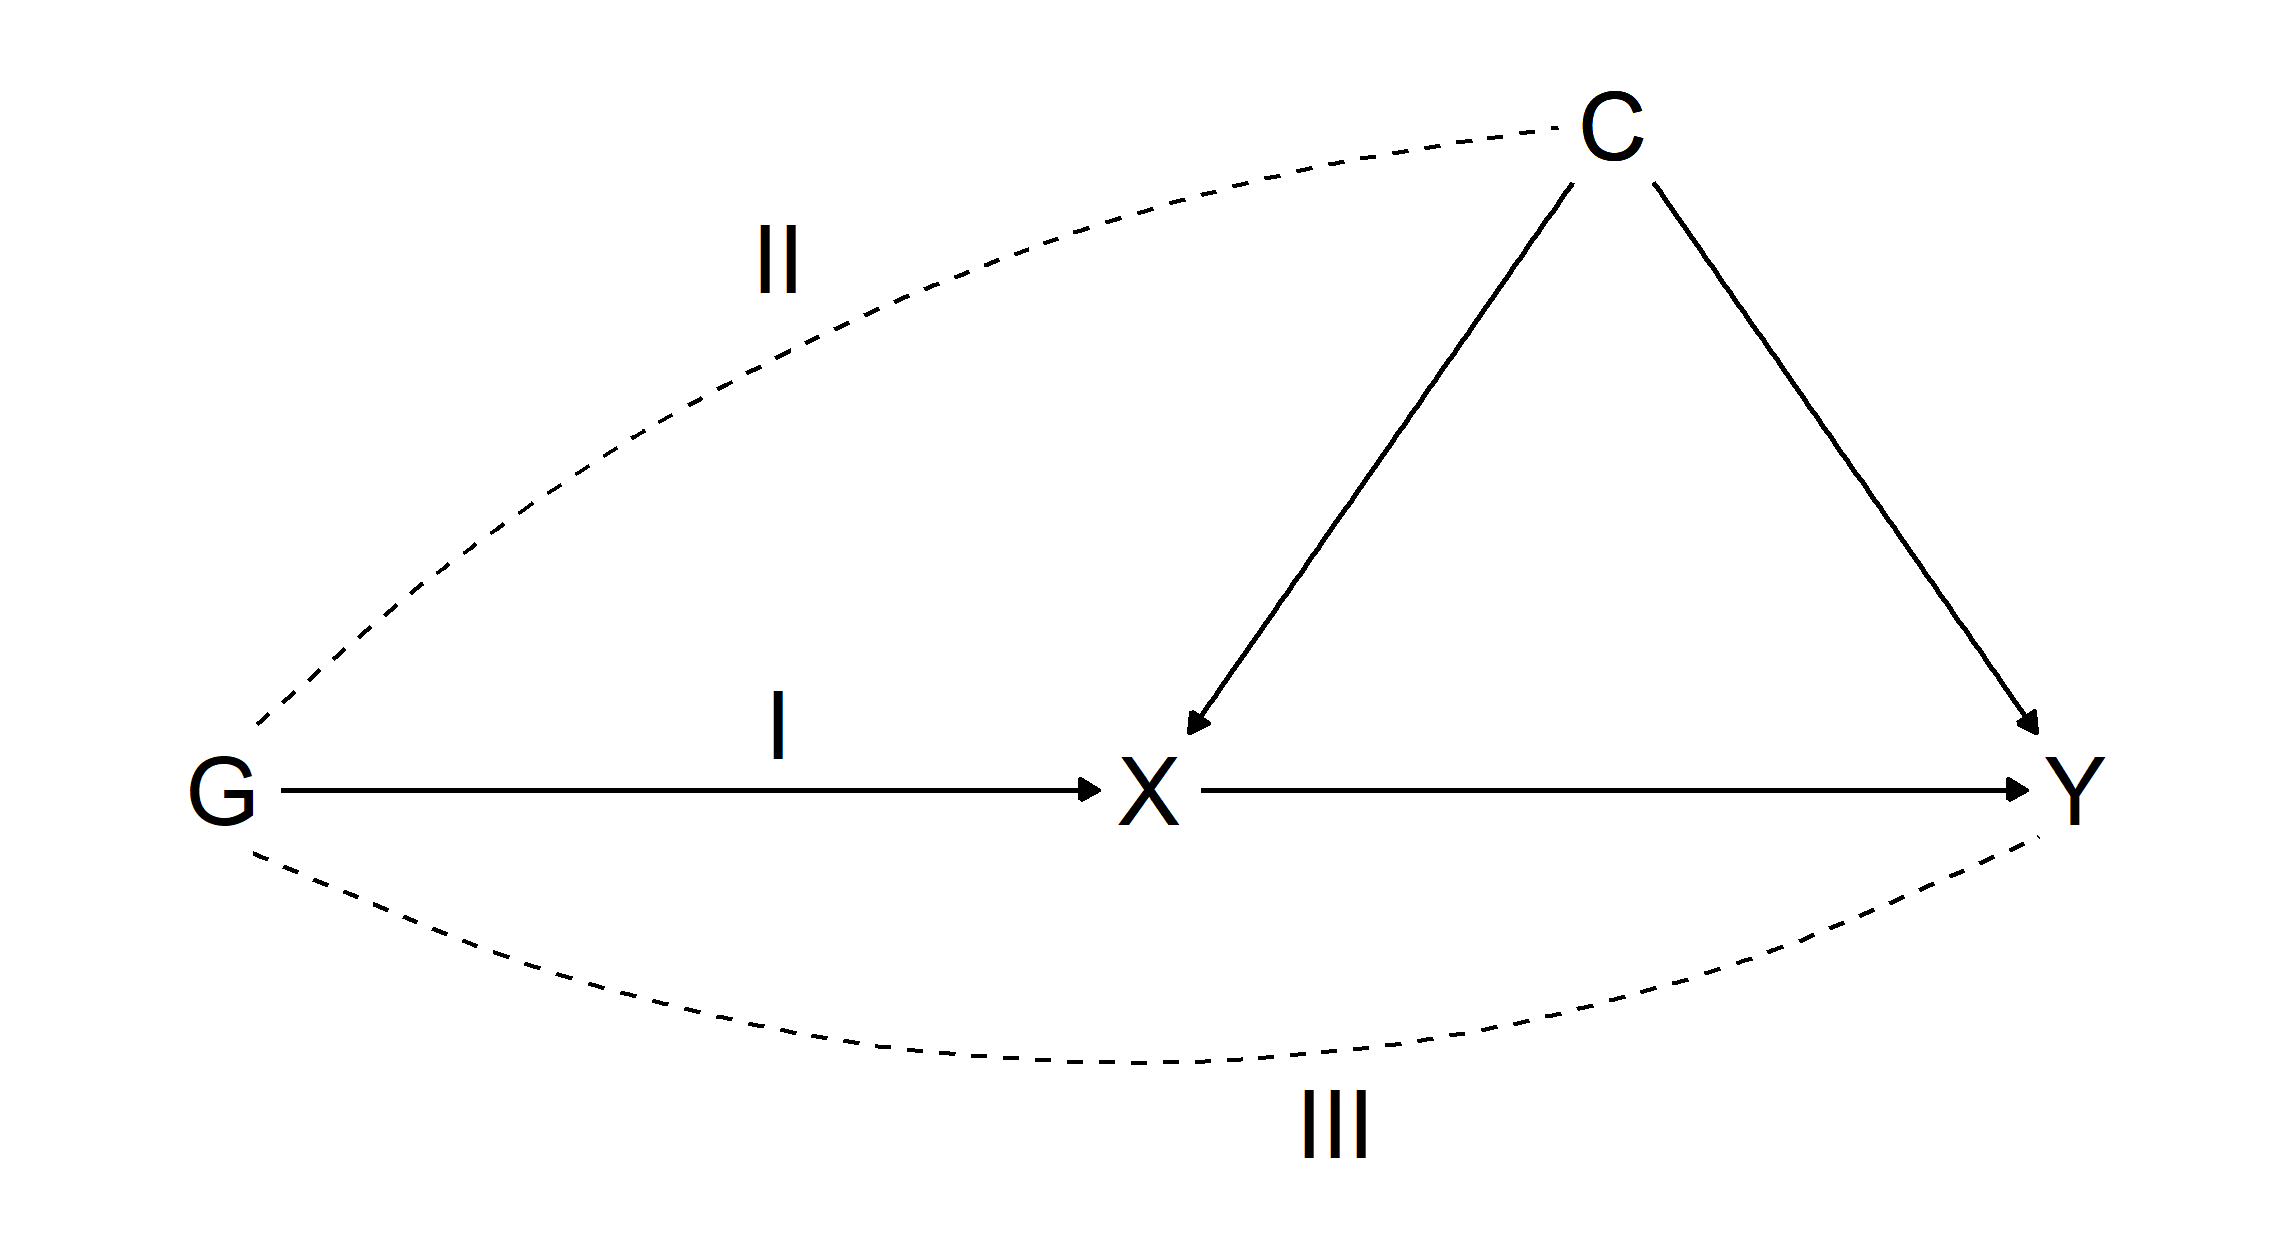
\includegraphics[width=0.7\linewidth]{figures/sys-rev/mrAssumptions} 

}

\caption[Overview of assumptions in Mendelian randomisation analyses]{Summary of the assumptions in Mendelian randomisation analyses: (I) \emph{relevance} - the genetic variant associates with the risk factor of interest; (II) \emph{independence} - the variant-exposure association has no unmeasured confounders; and (III) \emph{exclusion restriction} - variants affect the outcome only through their effect on the risk factor of interest (i.e.~there is no horizontal pleiotropy).}\label{fig:mrAssumptions}
\end{figure}

Firstly, this study design is relatively new, particularly when compared to randomised trials or cohort studies. Figure \ref{fig:typeByYear} demonstrates that Mendelian randomisation studies only begin to appear in the evidence base much later than NRSE/NRSI, likely due to the limited availabilt of large scale GWAS datasets needed for two-sample Mendelian randomisation analyses. As such, the process and tools for systematically assessing this study design are not as well developed. A key example of this is in the absence of validated search filters for Mendelian randomisations studies. This limitation is further complicated by the varying terminology used to describe the method, particularly in the early years of it's application, which lead o me including general terms for instrumental variable analyses in my search.

Additionally, there is currently no widely used risk-of-bias assessment tool for Mendelian randomisation studies. A recent commentary provided a checklist interpreting Mendelian randomisation studies, this guide includes reporting items in their quality checklist. While reporting quality is important, it is a separate consideration to internal validity, as discussed in Section \ref{risk-of-bias}. Similarly, a previous review of Mendelian randomisation studies used the Q-Genie tool which was validated to assess the quality of genetic association studies in meta-analysis.\textsuperscript{\protect\hyperlink{ref-sohani2015}{248}} While this tool assesses the underlying GWAS used, it does not assess the additional methodological considerations of the Mendelian randomisation analysis itself. For this review, I utilised the best available author-devised tool, sourced from a recent review of systematic reviews of Mendelian randomisation studies.

As a further stumbling block, Mendelian randomisation, particularly when using a two-sample summary data design, is a form of analysis that lends itself to multiple exposure-outcome comparisons. This is particularly relevant to the consideration of bias due to missing evidence. As an example, through snowballing and other measures, I identified at least one relevant Mendelian randomisation study that had not been identified by the search strategy.\textsuperscript{\protect\hyperlink{ref-larsson2017b}{249}} On review of this paper, the search would not have been expected to find it given the absence of any lipid-related keywords in the title and abstract. The study examined the association between lipid fractions with Alzheimer's disease as one of many risk factors for the condition. Studies such as this can introduce bias into a systematic review, as it is commonly only those risk factors that show a statistically significant result that are reported in the abstract and so are captured by the search. This may bias systematic reviews, including this one, as the analysis of multiple risk factors against a single outcome within a single publication becomes more common. These studies are described as ``unknown unknown's'' in the context of the RoB-ME tool, and are particularly challenging (as opposed to an analysis that was insufficiently reported to be included in the statistical analysis, or the ``known unknown's'').

Useful future work to improve the methodology for inclusion of Mendelian randomisation studies in systematic reviews should involve the development of a validated search filter for this study design.\textsuperscript{\protect\hyperlink{ref-waffenschmidt2020}{250},\protect\hyperlink{ref-wagner2020}{251}} Alternatively, in better-resourced reviews, a dedicated search for ``risk factors'' and ``dementia'' and ``Mendelian randomisation'' followed by manual review of studies that look across multiple risk factors would be advisable. This was not feasible in the context of this review, given the large number of records to be screened even when using study design filters (n=16,109). Additionally, the value of methods that supporting the traditional bibliographic database search, such as snowballing (forwards and backwards citation chasing) and communication with relevant topic experts should not be underestimated. Finally, development of a risk-of-bias assessment tool for this study design by a panel of methodologists and analysts would be of substantial benefit to the field.

One item of particular interest is the attenuation of any effects observed by Mendelian randomisation studies following the adjustment for/exclusion of genetic variation in the Apoe4 gene region. As covered in the introduction (see Section \ref{intro-basic-science}), an increasing number of ApoE4 alleles is a major independent risk factor for Alzheimer's disease, and so violates the exclusion restriction criteria (Figure \ref{fig:mrAssumptions}). In all cases, excluding these variants attenuates the observed effect to the null. A clear example of this is Benn \emph{et al} (2017), where the ApoE variants were not sufficient identified and excluded and the published paper detailed evidence for a protective effect of LDL-c was identified (RR: 0.83, 95\%CI: 0.75-0.92).\textsuperscript{\protect\hyperlink{ref-benn2017}{66}} Following several rapid responses, the data was re-analysed excluding a larger area around ApoE4 which attenuated the finding to the null.\textsuperscript{\protect\hyperlink{ref-benn2017a}{252}}

~

\hypertarget{inclusion-of-preprints}{%
\subsection{Inclusion of preprints}\label{inclusion-of-preprints}}

As highlighted in Section \ref{diverse-sources-preprints}, this review explicitly sought to synthesize evidence across different publication statuses (preprinted vs.~published). Using the tool described in Chapter \ref{sys-rev-tools-intro}, two preprint serves related to health and biomedical sciences were search as part of this review. The small number of studies returned by the searches (or the absence of any relevant hits in the medRxiv database - see Figure \ref{fig:prisma-flow-fig}) is due to the timing of the preprint searches. The searches for this review were performed in mid-July 2019, but the medRxiv repository, an offshoot of the Epidemiology and Clinical Trials categories of the bioRxiv preprint server, only registered its first preprint 25th June 2019. As such, at the point it was searched, the medRxiv database contained only a very small number of records (n=148).





\begin{figure}[H]

{\centering 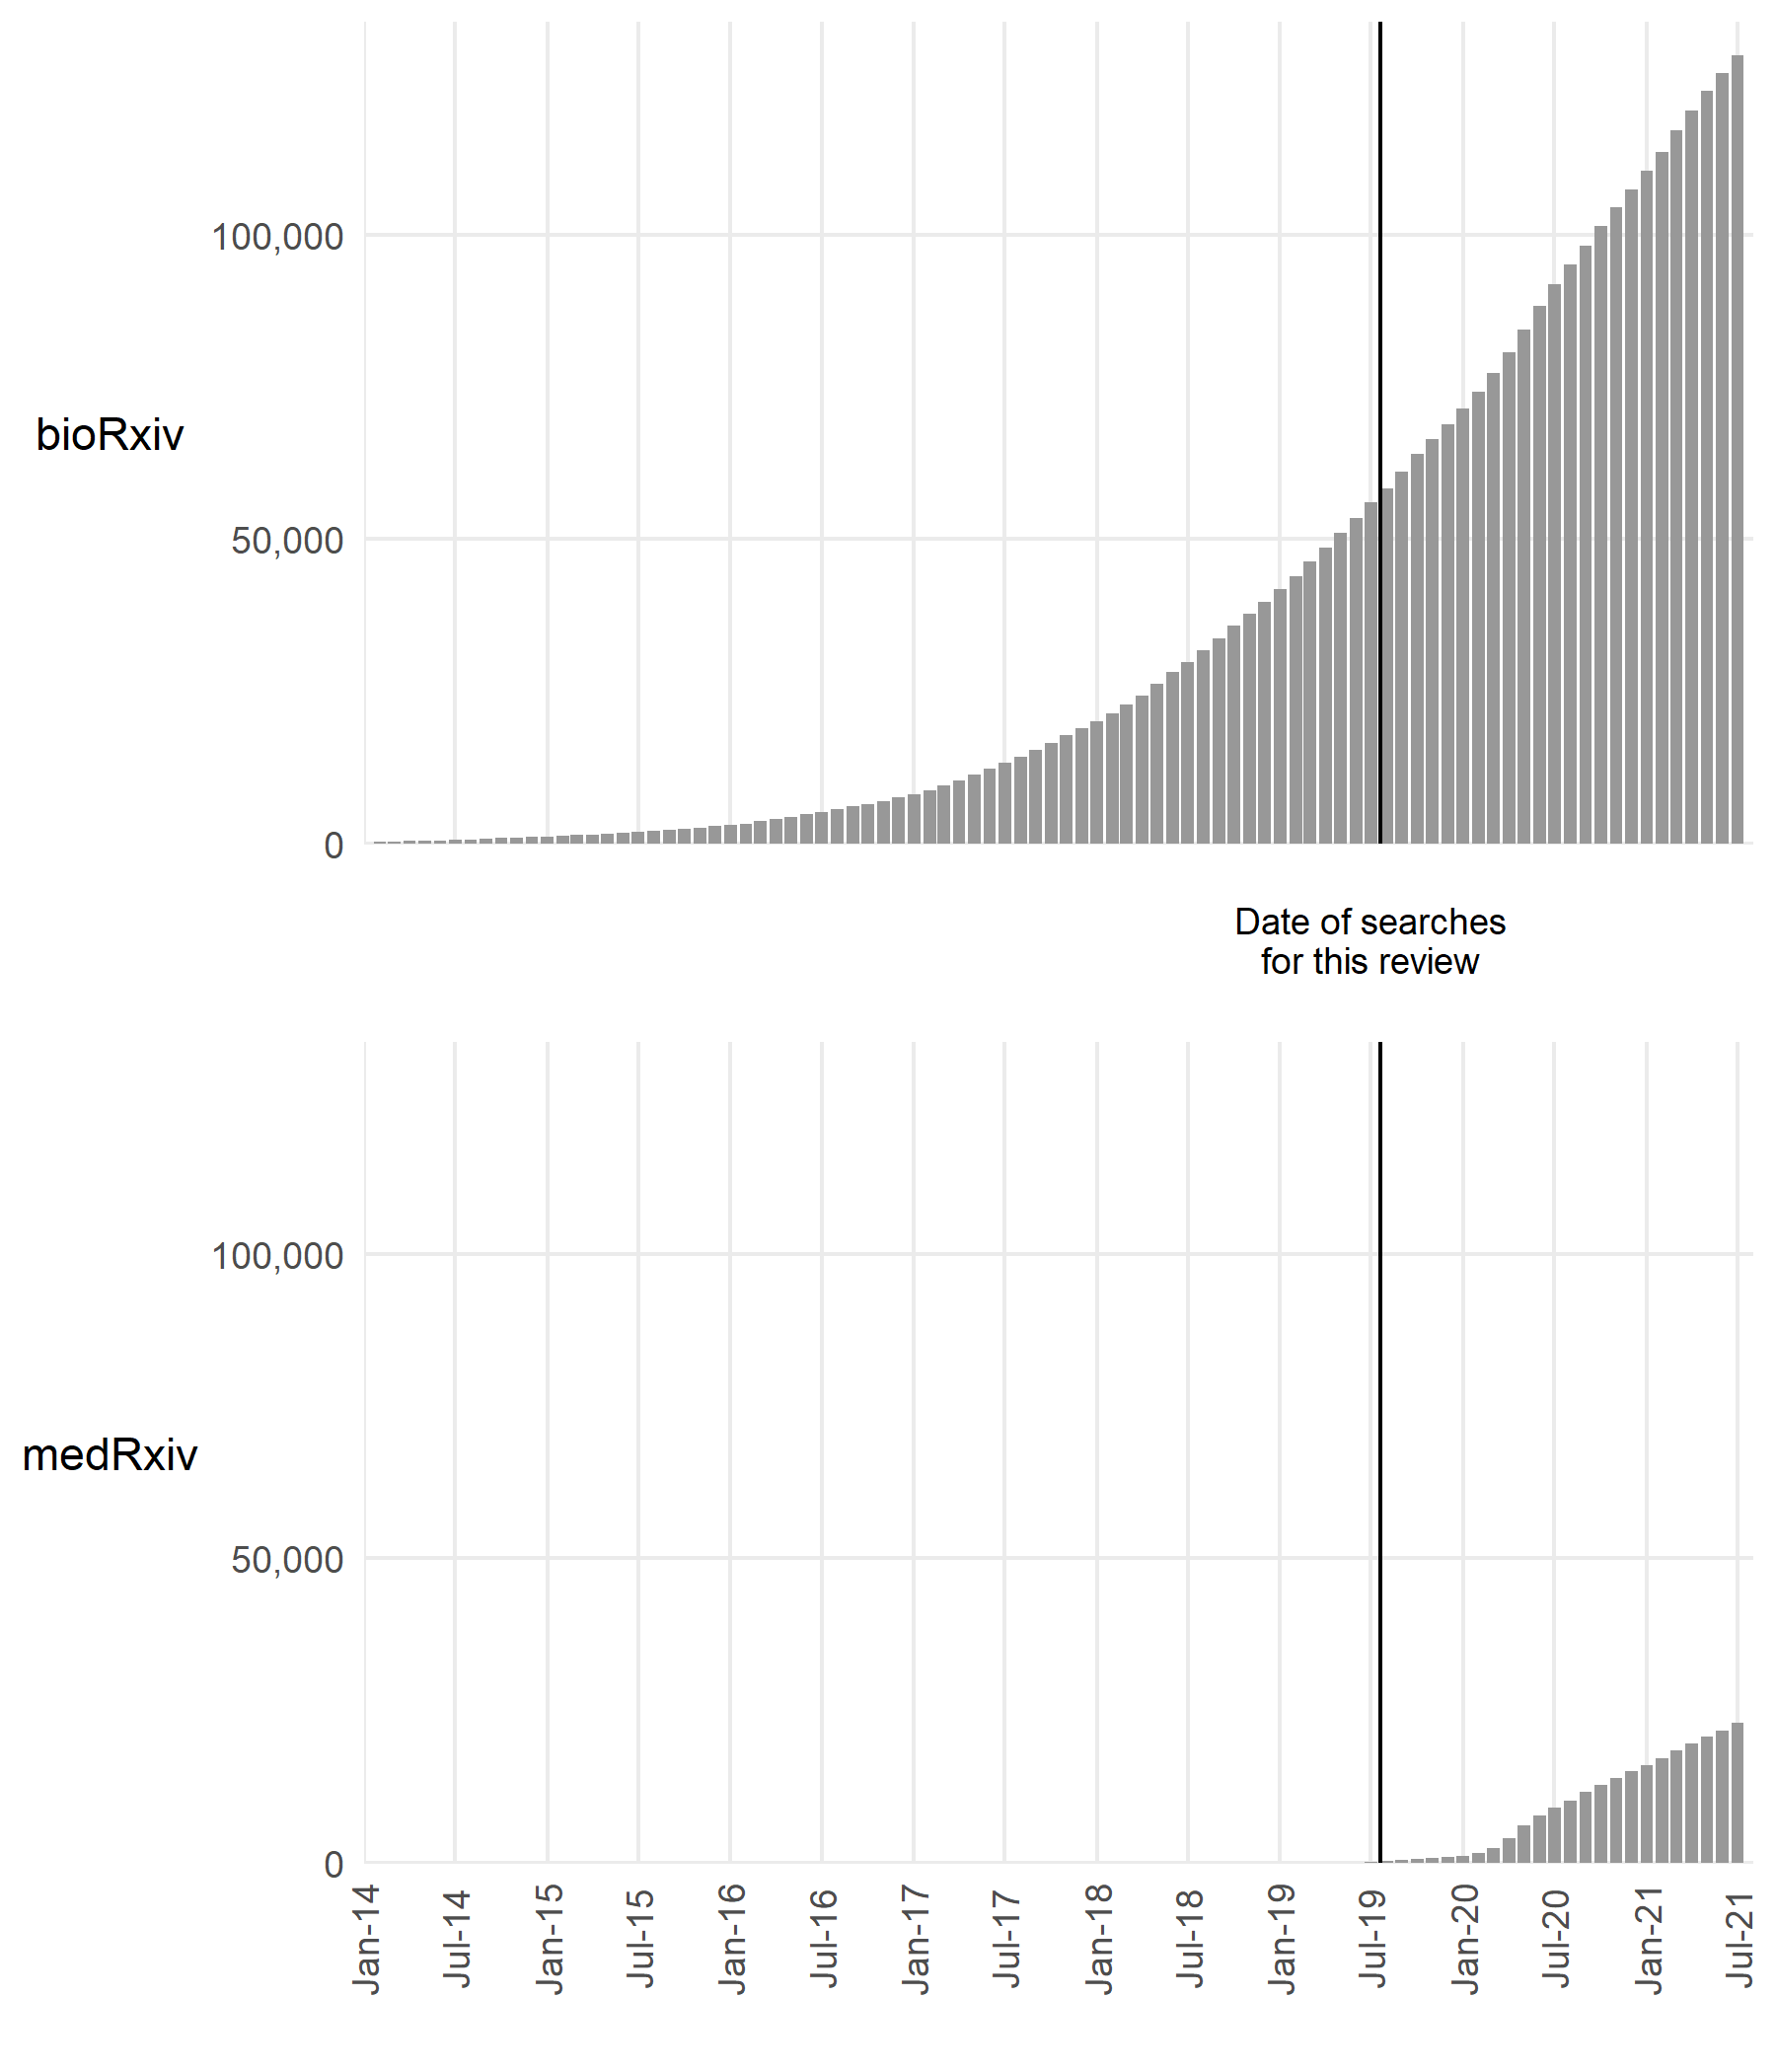
\includegraphics[width=0.8\linewidth]{figures/sys-rev/preprint_growth} 

}

\caption[Growth of preprint repositories over time]{Growth of preprint repositories over time. Given the relative sizes of the preprint repositories at the time the searches for this review were conducted (bioRxiv n= 56,007, medRxiv n = 148), the number of hits returned by each is expected.}\label{fig:preprintGrowth}
\end{figure}

Three relevant preprints from the bioRxiv hits were identified. The added evidential value of including these preprints was described in Section \ref{sys-rev-including-preprints-res}, and indicated that results available only via preprinted reports can contribute substantially to a meta-analysis. Of note, all three included preprints described Mendelian randomisation studies, potentially indicating that more biologically-focused study designs are over-represented in the bioRxiv repository.

Of the three identified preprints, two were subsequently published as of September 2020. This fits well with the analysis presented in Chapter \ref{sys-rev-tools-heading} that, allowing for a two-year lag, approximately two-thirds of preprints are published, and also nicely illustrates the dual advantages of preprinted reports to evidence syntheses.

Firstly, preprints provide an advance snapshot of the literature, capturing articles that will eventually be published but were not available at the time of the main search. Consider the example of one eligible preprint in this review was initially posted on bioRxiv in July 2019\textsuperscript{\protect\hyperlink{ref-andrews2019b}{253}} and was subsequently published in 2021 following peer-review.\textsuperscript{\protect\hyperlink{ref-andrews2021}{227}} Secondly, inclusion of preprints allows for results that may never be formally published to be included in an evidence synthesis exercise as is the case with the second preprint included in this review.\textsuperscript{\protect\hyperlink{ref-so2017}{232}} Both of these aspects illustrate that, if the aim is to find the current state of the art in the topic area at the time of searching, inclusion of preprints is a necessity.

More recently, inclusion of preprints in systematic reviews has become significantly more widespread. This is largely due to the role of preprint servers, in particular medRxiv, as a key evidence dissemination venue during the early stages of the COVID-19 pandemic.\textsuperscript{\protect\hyperlink{ref-fraser2020preprinting}{75}} How well this adoption of preprints will transfer to other less-urgent topics, where the speed of research does not put the same focus on preprinted articles, is currently unknown.

~

~

\hypertarget{sys-rev-open-data}{%
\subsection{Open data sharing}\label{sys-rev-open-data}}

As discussed in Section \ref{dose-response-results}, many primary studies did not report important information required for the dose-response meta-analysis, and so could not be included in the synthesis. This limitation was compounded by the expected low response rate to requests for further information from primary authors. While contacting authors is worthwhile, as it can substantially change the conclusion of a systematic review\textsuperscript{\protect\hyperlink{ref-meursingereynders2019}{254}} and is not too costly to systematic reviewers,\textsuperscript{\protect\hyperlink{ref-cooper2019}{255}} a far preferable option is that the authors of primary studies readily deposit all relevant study data at the point of publication.

Based on my experience of extracting data for this review, I co-authored a guidance article to aid primary prevention scientists in preparing and sharing their data so that it can easily be incorporated into a evidence synthesis exercise, using a trial of mindfulness interventions as an case study. A copy of this publication is available in Appendix \ref{published-papers}.\textsuperscript{\protect\hyperlink{ref-hennessy2021}{256}} In an attempt to apply my own guidance, I have invested a substantial amount of time and effort into making the data obtained by this review openly available to other researchers. \textbf{{[}Zenodo repository will be cited here{]}}

~

\hypertarget{strengths-and-limitations}{%
\subsection{Strengths and limitations}\label{strengths-and-limitations}}

\hypertarget{strengths}{%
\subsubsection{Strengths}\label{strengths}}

I believe there are several aspects where this review is distinct from those reviews already available in the published literature. While several reviews of this research topic exist,\textsuperscript{\protect\hyperlink{ref-chu2018}{57},\protect\hyperlink{ref-yang2020}{241}--\protect\hyperlink{ref-poly2020}{243}} the overlap between the list of studies included in each is not 100\%. As part of this review, I have not only performed a original search of primary literature databases, but have also screened the reference lists of comparable reviews to ensure no study has been omitted. In addition, this review employed a structured approach to risk-of-bias assessment using a domain-based tool. This repres important strength of this review, as the detailed risk of bias assessments are used in

Thirdly, as discussed at length in the section above, in contrast to other available reviews and enabled by the tool described in Chapter \ref{sys-rev-tools-heading}, this review systematically searched preprinted health-related preprints. Finally, as a secondary element, I used this review to pilot new research synthesis methodologies, in particular a new visualisation approach for risk-of-bias assessments and a forthcoming tool for assessing the risk-of-bias due to missing evidence.

~

\hypertarget{limitations}{%
\subsubsection{Limitations}\label{limitations}}

The primary limitation of this review is that several included studies used data from EHR databases, which come with serious concerns regarding validity\textsuperscript{\protect\hyperlink{ref-hsieh2019}{257}} \textsuperscript{\protect\hyperlink{ref-mcguinness2019validity}{258},\protect\hyperlink{ref-wilkinson2018}{259}} Relatedly, several studies which made use of electronic health record database did not report the specific code lists used, potentially introducing substantial heterogeneity between effect estimates. An empirical example of the effect of differing EHR code list is presented as part of the analysis in Chapter 4 (see Section \ref{comparing-codelists}).

In addition, the fact that only a sample of records were dual screened at the title/abstract and full-text stages is a potential limitation, as there is a chance that some eligible records could have been excluded. However, evidence from assessments of inter- and intra-rater reliability indicate that is is not a major concern.

One particular limitiation with regards to the risk-of-bias assessment is the fact that the ROBINS-E assessments were performed without the tool being finalised. This meant that there were no signalling questions to guide the domain-level risk-of-bias assessment, which may have influenced the accuracy with which domain-level judgements were assigned. However, there is no published empirical evidence supporting the need for signalling questions, and assessment of inter-rater reliability across the different tools did not indicate a specific problem with the ROBINS-E assessments. In fact, low agreement was common across the tools, though this is expected based on the available literature.\textsuperscript{\protect\hyperlink{ref-jeyaraman2020}{260}}

One further limitation is the fact that the risk of bias due to missing evidence assessment, combined with some empirical evidence that some studies were missed by the search but contained relevant studies is a definite limitation of this review (see Section @Ref(rev-discussion-MR) above for a fuller discussion of this issue with respect to Mendelian randomisations studies). Unfortunately, this is probably a common limitation across all reviews, based on the way in which increased sensitivity must be balanced with a reasonable workload.

~

\hypertarget{conclusions}{%
\section{Conclusions}\label{conclusions}}

In this chapter I have presented a comprehensive systematic review of the different sources of evidence available which examined the relationship between lipid levels and dementia use.

This work built on the tool introduced in the preceeding chapter (Chapter \ref(sys-rev-tools-heading)), and findings from this review are used though out the subsequent chapters: in Chapter \ref{cprd-analysis-heading}, summary of the evidence guided the choice of analysis approach, ensuring that the new analysis was at risk of a different source of bias; while in Chapter \ref{ipd-heading}, prospective cohorts identified by the review were contacted in an attempt to obtain individual participant data; finally, the cumulative effect measures calculated here are used as a key source of evidence for the triangulation exercise presented in Chapter \ref(discussion-heading).

\newpage

\hypertarget{references-2}{%
\section{References}\label{references-2}}

--- Archibald Cochrane, 2000\textsuperscript{\protect\hyperlink{ref-cochrane1979}{125}} --- Archibald Cochrane, 2000\textsuperscript{\protect\hyperlink{ref-cochrane1979}{125}}

\hypertarget{sys-rev-results-heading}{%
\chapter{Systematic review of all available evidence on the association between blood lipids and dementia outcomes}\label{sys-rev-results-heading}}

\minitoc 



\hypertarget{cprd-analysis-heading}{%
\chapter{Primary analysis of lipid-regulating agents and dementia outcomes}\label{cprd-analysis-heading}}

\minitoc 

\hypertarget{lay-summary-3}{%
\section{Lay summary}\label{lay-summary-3}}

Electronic health record (EHR) databases are large collections of medical data, used to manage patient administration and care. Under these systems, whenever a patient attends their GP, their clinical data is recorded in a central database using a standardised coding system. These databases have several advantages over traditional methods of data collection, including the number of people they contain and the length of time for which participants are followed. This is particularly important when studying diseases such as dementia, which may begin to develop in patients long before symptoms are seen.

This analysis makes use of the Clinical Practice Research Datalink (CPRD), which contains the electronic medical records of more than 3 million people from general practices across England. Using this data, the analysis presented in this chapter examined whether treatments which lower cholesterol levels (also known as lipid-regulating agents or LRA) of which statins are a prime example, affect the risk of all-cause dementia and related outcomes (Alzheimer's disease, vascular dementia and other dementias).

Little evidence for an effect of lipid-regulating agents effect on the risk of Alzheimer's disease was found, with the exception of a slightly increased risk in those prescribed a certain type of lipi-regulatin agent called fibrates. In contrast, I found an increased risk of vascular and other (i.e.~non-Alzheimer's) dementia was associated with lipid-regulating agent use.

This increased risk in outcomes with a vascular element (e.g.~vascular dementia) is unexpected, and is very likely to be due to the presence of bias in the analysis. This bias, called ``confounding by indication'', is caused when those who are prescribed a statin are more at risk of vascular dementia for a range of reasons, which makes it appear as if statins are harmful. Despite this limitation, the analysis presented provides an important source of information which will be used in later chapters.

~

\hypertarget{introduction-1}{%
\section{Introduction}\label{introduction-1}}

In this Chapter, I present an analysis of a large population-based electronic health record dataset to investigate the relationship between lipid-regulating agent (LRA) use and dementia outcomes. The analysis aims to address important two limitations of the current evidence base as identified by the systematic review presented in Chapter \ref{sis-rev-heading}.

Firstly, it explicitly examines vascular dementia as an outcome. The systematic review presented in the previous chapter identified an evidence gap around the effect of lipid-regulating agents on the risk of vascular dementia. As triangulation exercises require as many diverse sources of evidence as possible, this analysis provides a source of information on this outcome.

Secondly, and in a similar vein, the analysis intentionally takes a different analytical approach to that most commonly used to examine the effect of statins on dementia as identified by the systematic review. Specifically, this involved a concerted effort to address immortal time bias though use of a Cox proportional hazards analysis, incorporating a time-varying treatment indicator.\textsuperscript{\protect\hyperlink{ref-suissa2008}{262}} This approach provides a evidence source at risk of a distinct bias due to the alternative analytical strategy. The results from this analysis will be incorporated into the triangulation exercise presented in Chapter \ref{discussion-heading}.

This chapter represents an extended version of a preprint manuscript, a copy of which is available in Appendix \ref{published-papers}.

~

\hypertarget{methods-1}{%
\section{Methods}\label{methods-1}}

\hypertarget{study-protocol}{%
\subsection{Study protocol}\label{study-protocol}}

An \emph{a priori} protocol for this study was published,\textsuperscript{\protect\hyperlink{ref-walker2016}{263}} and amendments to this are recorded in Appendix \ref{appendix-cprd-amendments}.\textsuperscript{\protect\hyperlink{ref-vonelm2008}{264}}

~

\hypertarget{cprd-data-source}{%
\subsection{Data source}\label{cprd-data-source}}

Previously known as the General Practice Research Database (GPRD), the Clinical Practice Research Datalink (CPRD) is a large population-based electronic health record (EHR) database.\textsuperscript{\protect\hyperlink{ref-herrett2015}{265}} The database has been collecting primary care data from participating practices across England since 1987.\textsuperscript{\protect\hyperlink{ref-williams2012}{266},\protect\hyperlink{ref-wood2001revitalizing}{267}} It contains the primary care records for more than 10 million primary care patients in England, and is broadly representative of the UK population in terms of age, sex and ethnicity.\textsuperscript{\protect\hyperlink{ref-herrett2015}{265},\protect\hyperlink{ref-mathur2014}{268}}

To avoid the ambiguity of interpreting free-text clinical notes and to allow for easy analysis of the resulting data, the CPRD primarily collects data using a predefined coding system known as Read codes.\textsuperscript{\protect\hyperlink{ref-booth1994}{269}} All clinical events, included clinical test results and diagnoses, can be identified by a specific Read code. The codes use a nested approach (see Table \ref{tab:readExample-table}), with the initial characters defining broad diagnostic topics (e.g.~Eu\ldots{} - Mental and behavioural disorders), while subsequent characters provide additional information on the specific condition diagnosed (e.g.~Eu001 - Dementia in Alzheimer's disease with late onset).

~





\begin{table}[H]

\caption[Example of CPRD Read code hierarchy]{\label{tab:readExample-table}Example of CPRD Read code hierarchy, showing how ``Dementia in Alzheimer's disease with late onset'' (\emph{Eu001}) is nested under the top-level of ``Mental disorders'' (\emph{Eu\ldots{}}). Broad topics are specified using the initial two alpha-numeric characters of the Read code, while subsequent characters are used to define specific conditions and context.}
\centering
\begin{tabular}[t]{cll}
\toprule
\textbf{Level} & \textbf{Read code} & \textbf{Term}\\
\midrule
1 & E.... & Mental disorders\\
2 & Eu... & Mental and behavioral disorders\\
3 & Eu0.. & Organic mental disorder\\
4 & Eu00. & Dementia in Alzheimer's disease\\
5 & Eu001 & Dementia in Alzheimer's disease with late onset\\
\bottomrule
\end{tabular}
\end{table}

~

The index events, exposures and outcomes used in this analysis were identified using predetermined code lists, which are available for inspection from the archived repository accompanying this analysis (data/code availability is discussed in Section \ref{cprd-data-avail}).

~

\hypertarget{cohort-definition}{%
\subsection{Cohort definition}\label{cohort-definition}}

This analysis included all participants registered at a participating practice between 1 January 1995 and 29 February 2016 who had a flag for ``research quality'' data. Records pre-dating the 1995 cut-off were included in the original CPRD extract obtained for this analysis. However, these were excluded from the analysis as data quality and reliability are thought to be higher after this date.\textsuperscript{\protect\hyperlink{ref-wolf2019}{270}} Additionally, individuals with less than 12 months of continuous records prior to cohort entry were excluded, making the effective start date of the cohort 1 January 1996.

Participants were included in the study cohort if their record contained any of the following index events: a Read code for a diagnosis of hypercholesterolemia or related condition; a Read code for prescription of a lipid-regulating agent (such as statins); a total cholesterol test result of \textgreater4 mmol/L; or an LDL-c test result of \textgreater2 mmol/L.\textsuperscript{\protect\hyperlink{ref-walker2016}{263}} The blood lipid cut-offs were based on NIHR-recommended levels at the time the protocol was written. These index events allowed me to define a population of participants who were either at risk of hypercholesterolemia, as indicated by the elevated total or LDL cholesterol test results, or had already been diagnosed with it, as indicated by a diagnostic code/related prescription.

The index date for a participant was defined as the date where the first relevant code or test result was recorded on their clinical record, and participants were followed up until the earliest of: (a) an outcome of interest; (b) death; (c) end of follow-up (29 February 2016); (d) last registration date with their GP practice; or (e) the last CPRD collection date for their practice. Participants were ineligble for our cohort if they were less than 40 years of age (as these patients are are less likely to be prescribed a LRA), had less than 12 months of ``research quality'' data, were simultaneously prescribed more than one lipid-regulating agent (due to the difficult of assigning these to a single exposure group), or were diagnosed with an outcome of interest before or on the date of the index event (i.e.~had less than one full day of follow-up).

~

\hypertarget{exposures}{%
\subsection{Exposures}\label{exposures}}

We considered seven lipid-regulating drug classes based on groupings in the British National Formulary (BNF),\textsuperscript{\protect\hyperlink{ref-wishart2017}{271}} namely: statins, fibrates, bile acid sequestrants, ezetimibe, nicotinic acid groups, ezetimibe and statin (representing one treatment containing both drugs, rather than the two classes being prescribed concurrently), and omega-3 fatty acid groups.

A participants drug class was assigned based on their first recorded prescription, and any drug switching was ignored in an effort to mimic an intention-to-treat approach. We did however examine how often the initial drug class altered according to one of three criteria:

\begin{itemize}
\tightlist
\item
  \textbf{stopped}: defined as the last prescription of the primary class being followed by at least six months of observation;
\item
  \textbf{added}: defined as a second drug class being prescribed before the last prescription of the initial class; and
\item
  \textbf{switched}: defined as a second drug class being prescribed after the last prescription of the initial class.
\end{itemize}

~

\hypertarget{cprd-outcomes}{%
\subsection{Outcomes}\label{cprd-outcomes}}

We considered five outcomes as part of this analysis: probable Alzheimer's disease, possible Alzheimer's disease, vascular dementia, other dementias, and a composite all-cause dementia outcome. When two or more outcomes were coded in a participant's clinical record, a decision tree was used to differentiate between them (Figure \ref{fig:decisionTreeFig}). The diagnosis date of the outcome was determined by the first record of a relevant code.





\begin{figure}[H]
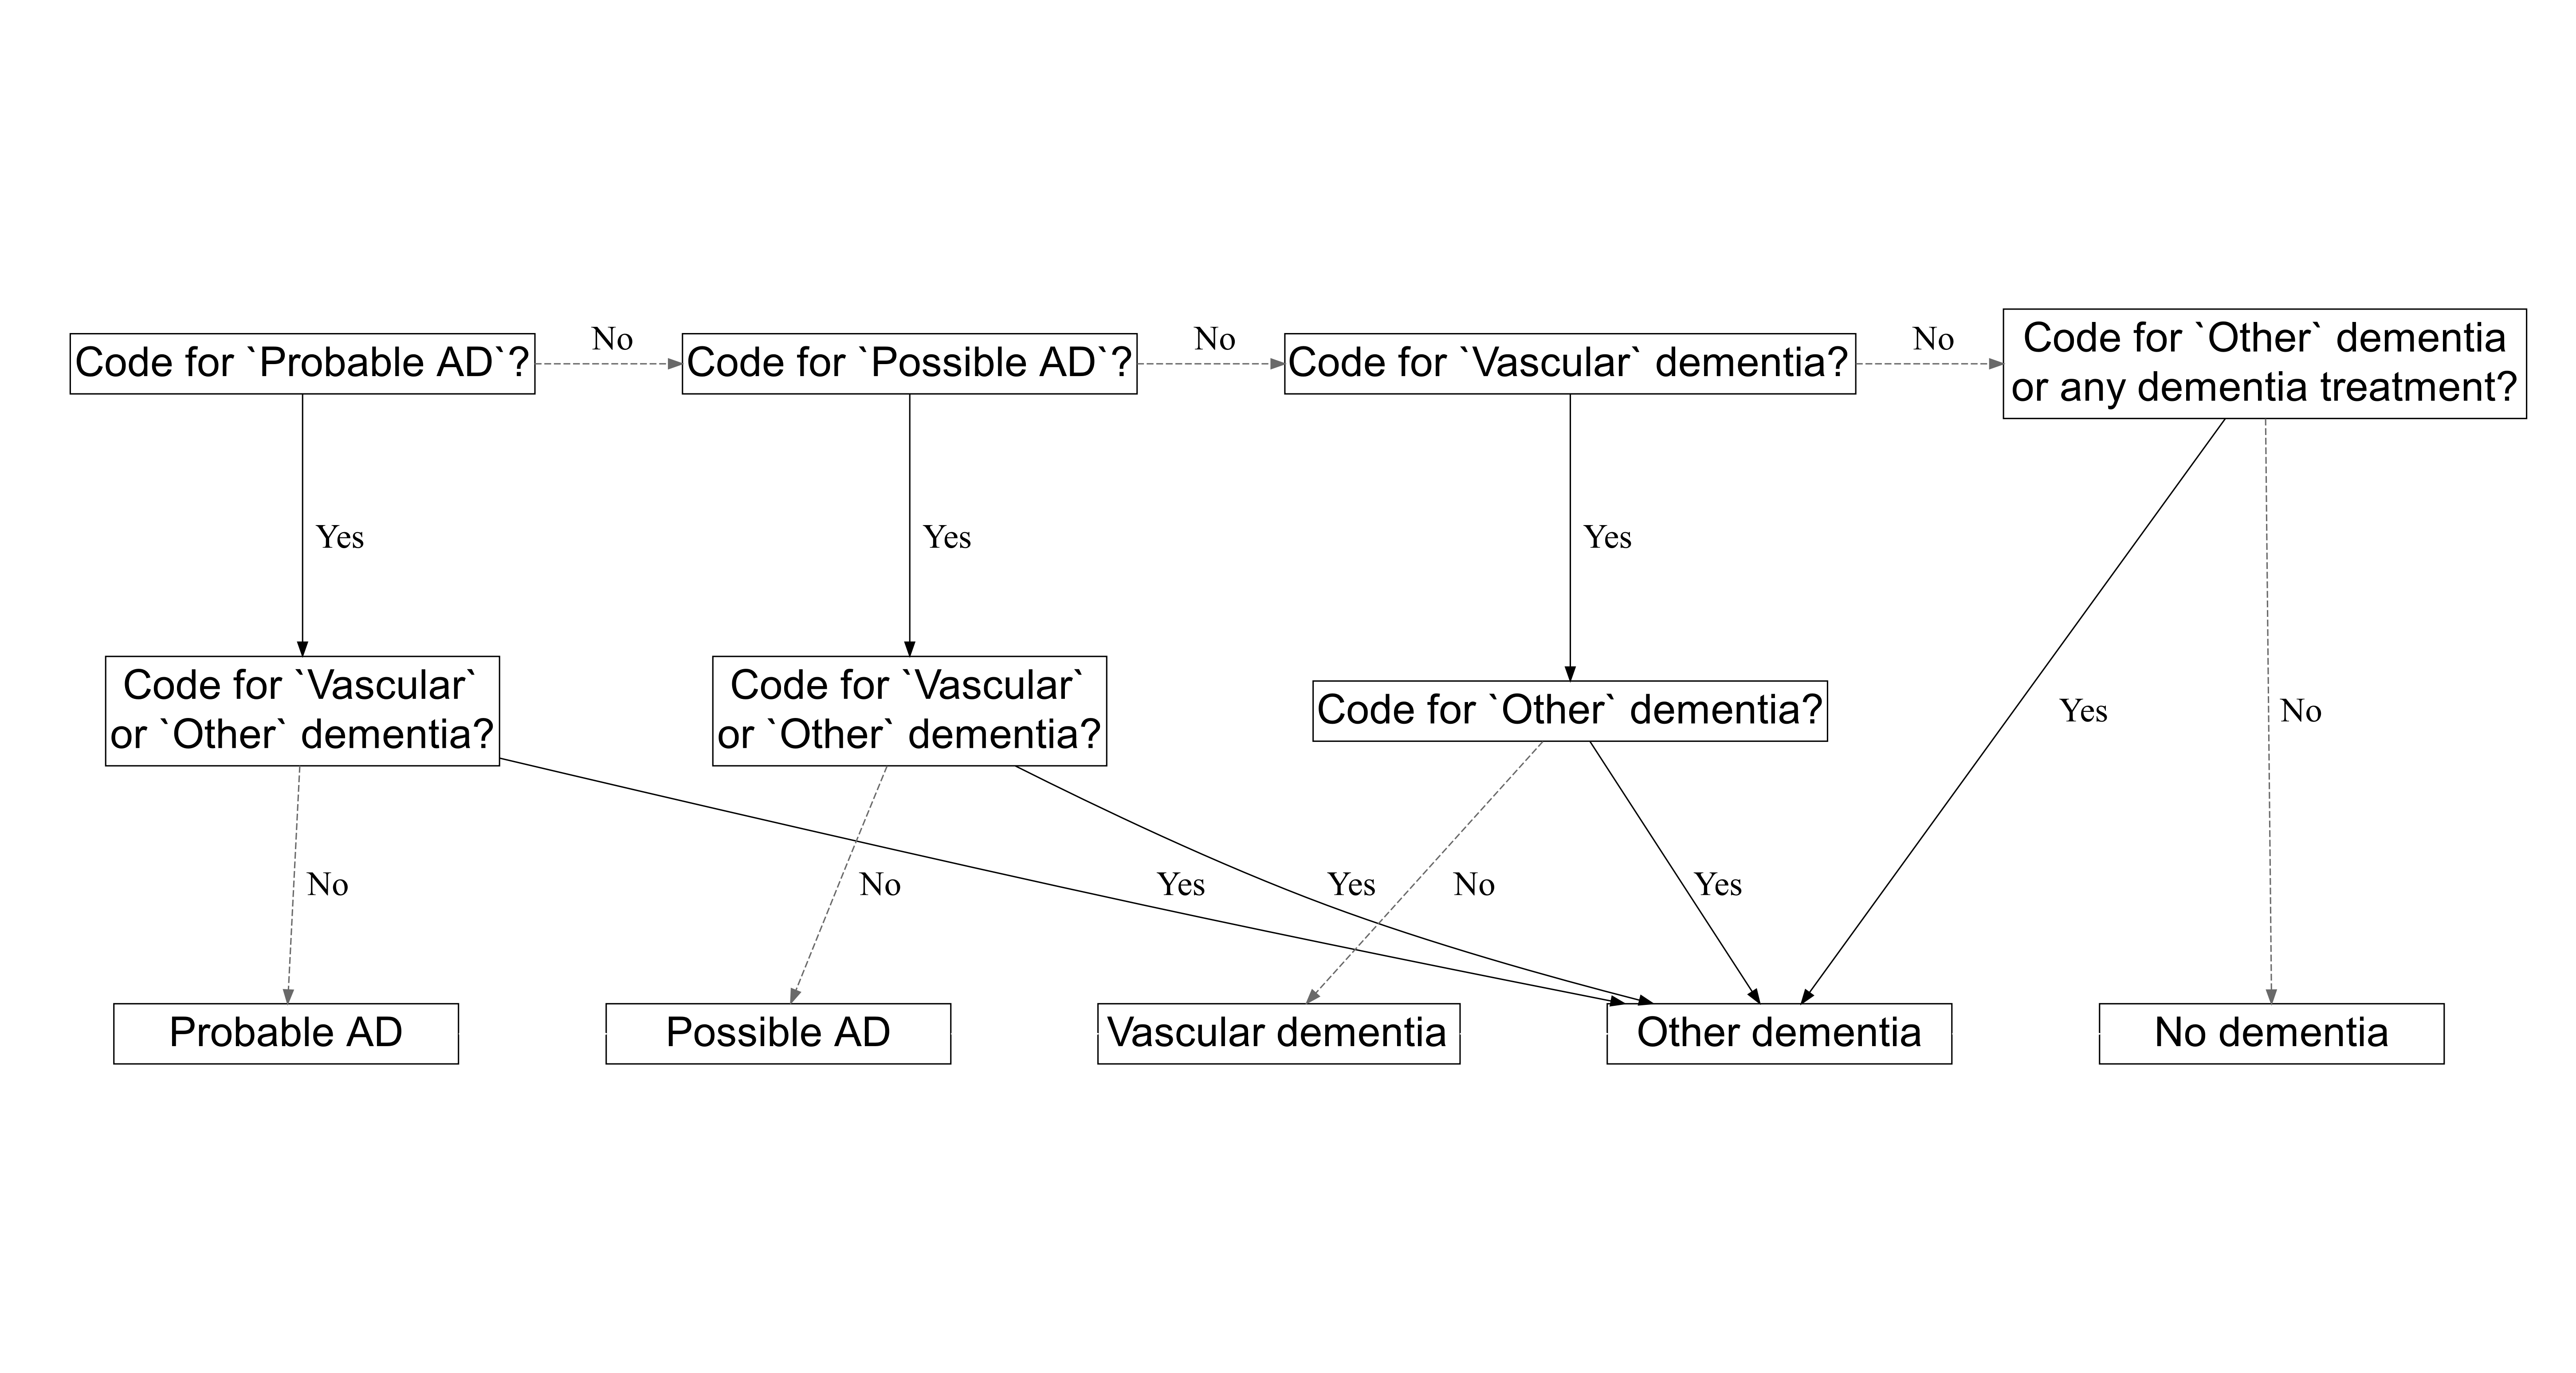
\includegraphics[width=1\linewidth]{figures/cprd-analysis/decision_tree} \caption[Decision tree for assigning dementia subtypes]{Decision tree for assigning dementia subtypes, based on the presence of Read codes in the patient's record. Note that an outcome of ``probable'' or ``Possible'' Alzheimer's disease (AD) requires the absence of any vascular outcome codes.}\label{fig:decisionTreeFig}
\end{figure}

~

\hypertarget{covariates}{%
\subsection{Covariates}\label{covariates}}

A range of additional variables were included in the analysis, intended to address the different distributions of potential confounding variables between those who were prescribed an lipid-regulating agent and those who were not. These are discussed in detail below and summarised in Table \ref{tab:covariateDef-table}.

~









Charlson index implemented using Read code lists.\textsuperscript{\protect\hyperlink{ref-khan2010}{273}} Code lists based on those by Taylor et al.\textsuperscript{\protect\hyperlink{ref-taylor2016}{274}}

\begin{table}[H]

\caption[Covariates adjusted for.]{\label{tab:covariateDef-table}Definition of covariates adjusted for in the full-adjusted model. The codelists used to define the majority of these covariates were originally created for use in a previously published analysis.\textsuperscript{\protect\hyperlink{ref-walker2020}{272}} while others were built on or adapted from previous published work,\textsuperscript{\protect\hyperlink{ref-khan2010}{273}--\protect\hyperlink{ref-wright2017}{275}}.}
\centering
\fontsize{9}{11}\selectfont
\begin{tabular}[t]{>{\raggedright\arraybackslash}p{15em}>{\centering\arraybackslash}p{25em}}
\toprule
\textbf{Covariate } & \textbf{How was the covariate defined?}\\
\midrule
Previous history of coronary arterial disease & Presence of one or more relevant Read codes on record.\\
\midrule
Previous history of coronary bypass surgery & Presence of one or more relevant Read codes on record.\\
\midrule
Previous history of cerebrovascular disease (including stroke) & Presence of one or more relevant Read codes on record.\\
\midrule
Chronic illness, including cancer and arthritis & Charlson index implemented using Read code lists.\textsuperscript{\protect\hyperlink{ref-khan2010}{273}} Code lists based on those by Taylor et al.\textsuperscript{\protect\hyperlink{ref-taylor2016}{274}}\\
\midrule
Socioeconomic position & 2010 English Index of Multiple Deprivation (IMD) at the twentile level, where 1 represents the least deprived and 20 the most deprived.\\
\midrule
\addlinespace
Consultation rate & Calculated by dividing the total number of clinic visits by the length of the patient record prior to the index date to give an average annual rate.\\
\midrule
Alcohol status & Recorded value (current, former or never).\\
\midrule
Smoking status & Most recent of recorded value (current, former or never) or Read code indicating a recorded value. Code lists based on those by Wright et al.\textsuperscript{\protect\hyperlink{ref-wright2017}{275}}\\
\midrule
Body Mass Index & Recorded value if available, or a calculated value using the last recorded height and weight measurements. Measurements taken before the age of 25 were excluded to ensure adult measurements were used.\\
\midrule
Peripheral arterial disease & Presence of one or more relevant Read codes on record.\\
\midrule
\addlinespace
Hypertension & Presence of one or more relevant Read codes on record.\\
\midrule
Baseline total cholesterol & Continuous value recorded as test result ("enttype==163 \& test\_data1==3")\\
\midrule
Baseline LDL cholesterol & Continuous value recorded as test result ("enttype==177 \& test\_data1==3")\\
\midrule
Chronic kidney disease & Presence of one or more relevant Read codes on record.\\
\midrule
Type 1 Diabetes & Presence of one or more relevant Read codes on record.\\
\midrule
\addlinespace
Type 2 Diabetes & Presence of one or more relevant Read codes on record.\\
\bottomrule
\end{tabular}
\end{table}

~

Demographic covariates adjusted for included age and gender. Age was calculated at date of entry into the cohort, and adjusted for via its use as the time axis for the Cox model (see Section \ref{cprd-time-axis}). Socioeconomic status was proxied using the Index of Multiple Deprivation (IMD) 2010, which draws on seven domains (income; employment; education, skills and training; health and disability; crime; barriers to housing and services; living environment) to create an overall deprivation score for each of 32844 statistical geography areas in England. To help preserve patient privacy, IMD score is only available from the CPRD in twentiles, with 1 indicating the least deprived and 20 indicating the most deprived. Smoking and alcohol use was determined at index, and participants were categorised as current, former, or never users of each.

Body mass index (a summary measure calculated as \(weight/height^2\)), baseline total cholesterol and baseline LDL cholesterol measures were obtained, using the last recorded value prior to the index date. A variable indicating grouped year of entry into the cohort (\textless=2000, 2001-2005, 2006-2010, \textgreater2010) was included to allow for changes in prescribing trends across the lifetime of the cohort. To assess healthcare utilisation, I adjusted for the average annual number of consultations between the beginning of a patients data and their entry into the cohort.

Finally, presence of a range of related conditions at baseline were accounted for, including cardiovascular disease, coronary bypass surgery, coronary artery disease, peripheral arterial disease, hypertension, chronic kidney disease, and Type 1 and Type 2 diabetes. In addition to adjusting for these covariates individually, a Charlson co-morbidity index (CCI) score was calculated for each participant. The CCI is a weighted index that uses presence and severity of a number of conditions to enable adjustment for the general health of a participant in terms of their mortality risk.\textsuperscript{\protect\hyperlink{ref-charlson1987new}{276}} Inclusion of this index allowed me to attempt to adjust for the general health of patients included in the analysis.

Codelists for all covariates can be found in the archived data repository accompanying this analysis (see Section \ref{cprd-data-avail}).

~

\hypertarget{missing-data}{%
\subsection{Missing data}\label{missing-data}}

Missing data are a recognised issue in electronic health records databases,\textsuperscript{\protect\hyperlink{ref-wells2013strategies}{277}} given that they contain administrative data, collected primarily for the purposes of patient management and care rather than academic research.

In this analysis, missing data were handled using a multiple imputation approach.\textsuperscript{\protect\hyperlink{ref-sterne2009}{278}} Variables with missing observations were identified for inclusion in the imputation model. Nominal variables with missing values were modelled using multinomial logistic regression, while continuous variables were modelled using linear regression. As per best practice, all variables used in the analytic model, including the outcome, were included in the imputation model.\textsuperscript{\protect\hyperlink{ref-moons2006using}{279}} Using the MICE (Multiple Imputation by Chained Equations) command in STATA16, 20 imputed datasets were created.

Missing data was only considered an issue for variables where a numerical test result was expected (e.g.~BMI), or where a code existed for the absence of the condition (e.g.~categorical smoking status). This approach was necessary, as absence of a code for other treatments or conditions (e.g.~statin use or dementia) was assumed to indicate absence of the treatment/condition rather than being considered missing.\textsuperscript{\protect\hyperlink{ref-wells2013strategies}{277}}

~

\hypertarget{estimation-methods}{%
\subsection{Estimation methods}\label{estimation-methods}}

A Cox proportional hazards (PR) model was used to estimate the effect of statins on dementia outcomes. Cox PR models are defined in general terms as:

\begin{equation}
  h(t) = h_o(t) \times exp(b_1x_1 + b_2x_2 + ... +b_px_p)
  \label{eq:cox-model}
\end{equation}

where:

\begin{itemize}
\tightlist
\item
  \(t\) is the survival time;
\item
  \(h(t)\) is the hazard function; and
\item
  \(x_1,x_2,...,x_p\) are the covariates which determine the hazard function, while \(b_1,b_2,...,b_p\) are the coefficients for each covariate.
\item
  \(h_o(t)\) is the baseline hazard - when all \(x_i\) are zero, the \(exp()\) function resolves to 1.
\end{itemize}

A Cox PR model was chosen for this analysis as it inherently accounts for the length of time participants spend in each exposure group. Using this approach, time-at-risk can be properly attributed to the appropriate exposure group, thus mitigating the impact of immortal time bias. This is discussed in detail in the following section.

~

\hypertarget{cprd-immortal-time-bias}{%
\subsection{Immortal time bias and time-varying treatment indicators}\label{cprd-immortal-time-bias}}

Immortal time bias describes two distinct but related types of bias. The first presentation, the selection bias aspect (Panel A, Figure \ref{fig:immortalTimeBias}), occurs when time prior to the exposure is excluded leading to the exposed and control groups being followed up from different time points.\textsuperscript{\protect\hyperlink{ref-levesque2010}{280}} Following the example displayed in the figure, the unexposed group are followed from the date of a diagnosis, while the exposed group is followed from date of a prescription. In this scenario, the time between diangosis and prescription for the exposure group is missing, and any events that occur in the exposed group prior to the prescription will be inappropriately excluded from the analysis.

The second presentation of immortal time bias is as a type of misclassification bias (Panel B, Figure \ref{fig:immortalTimeBias}). It occurs when the exposure time prior to the prescription, and any events occurring within it, is inappropriately assigned to the exposed group.

~





\begin{figure}[H]
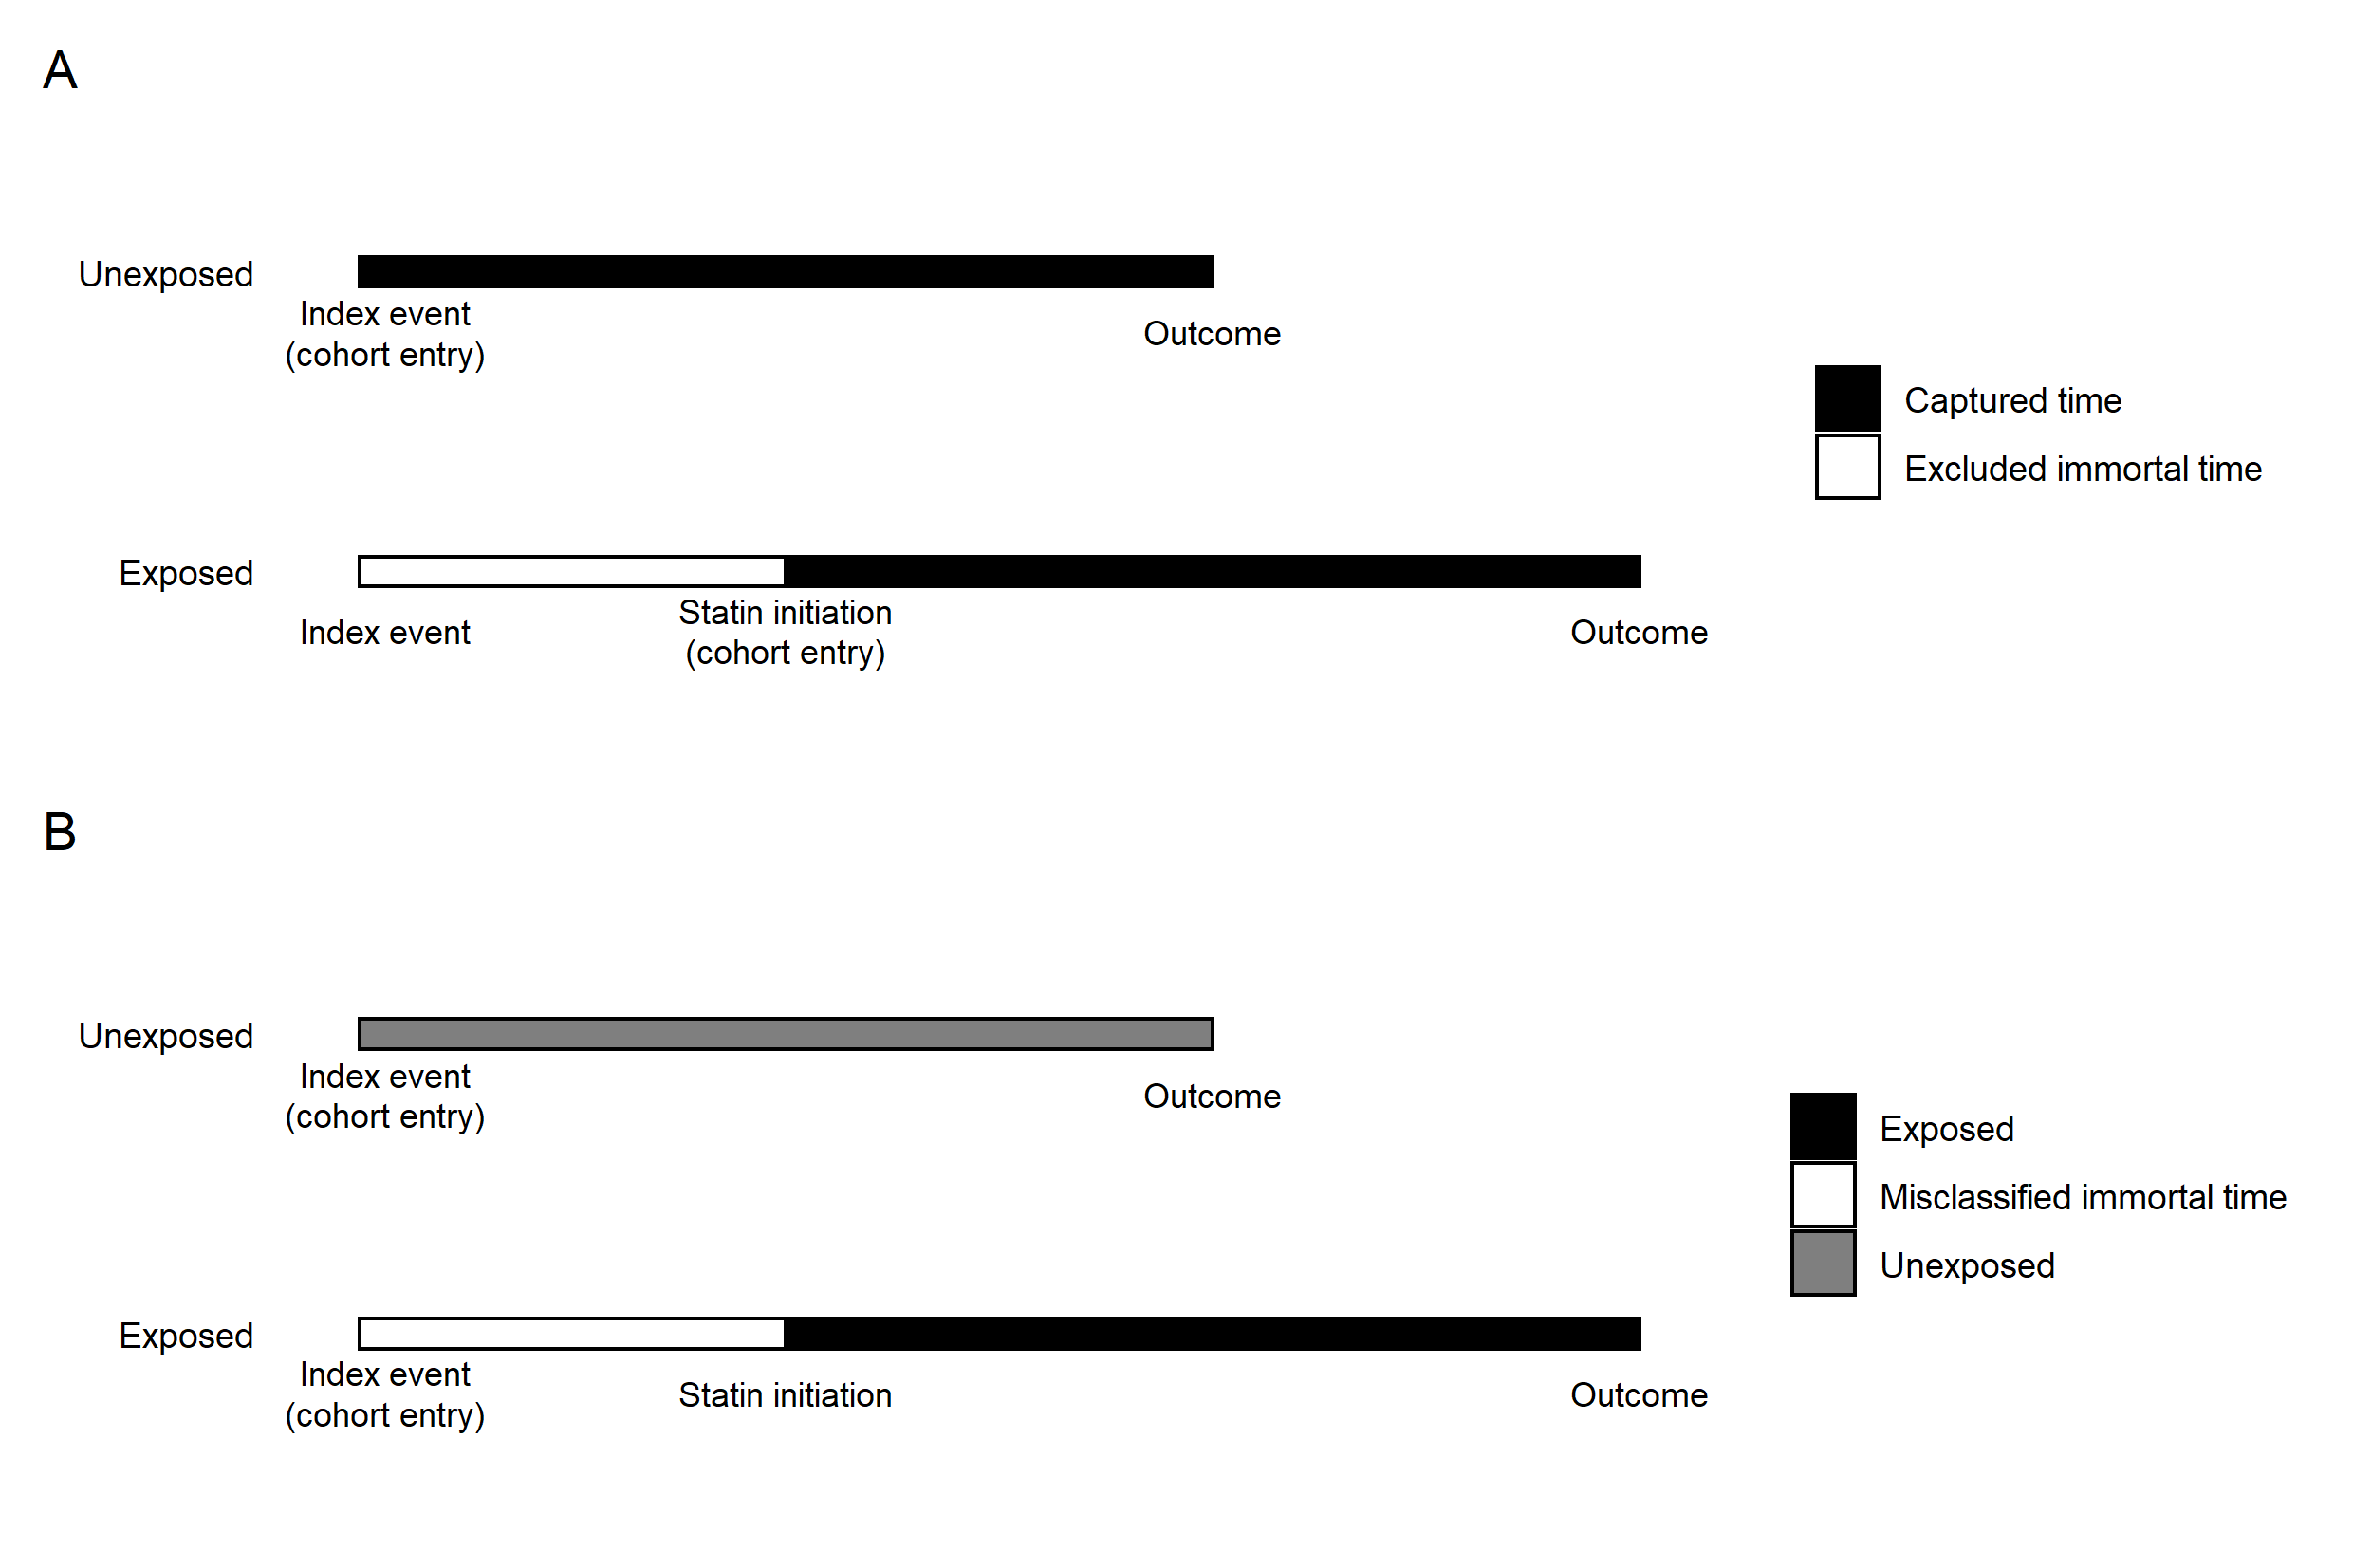
\includegraphics[width=1\linewidth]{figures/cprd-analysis/immortal_time} \caption[shortcap]{Diagram illustrating the two presentations of immortal time bias, as a selection bias (Panel A) and a misclassification bias (Panal B).}\label{fig:immortalTimeBias}
\end{figure}

~

This second presentation appears to be common in the existing literature, as several of the studies included in the systematic review presented in Chapter \ref{sys-rev-heading} were identified as being at risk of immortal time bias following formal risk of bias assessment using the ROBINS-I tool (see Section \ref{risk-of-bias-subheading}). Both presentations of immortal time bias appear in the literature on the relationship of statins and dementia, as identified by the systematic review presented in Chapters \ref{sys-rev-methods-heading}/\ref{sys-rev-results-heading}

This analysis attempted to address this issue by following all participants from a common index date (defined as earliest of: (a) date of raised cholesterol test results; (b) hypercholesterolemeia diagnosis; or (c) LRA prescription). Following a recommended approach to addressing the second form of immortal time bias, I employed a time-varying indicator of treatment status to correctly allocate time-at-risk to the exposed and unexposed groups.\textsuperscript{\protect\hyperlink{ref-levesque2010}{280}}

Under this approach, all patients start in the unexposed group and contribute time-at-risk until they are prescribed a lipid-regulating agent and move into the exposed group. Note, patients for whom prescription of a lipid-regulating agent was the index event only contribute time to the exposed group (i.e.~they enter the cohort and move into the exposed group on the same day).

~

\hypertarget{cprd-time-axis}{%
\subsection{Time axis}\label{cprd-time-axis}}

As part of a Cox proportional hazard model, there is the option to use either absolute time in cohort or participants age as the time scale of interest.\textsuperscript{\protect\hyperlink{ref-lamarca1998}{281}--\protect\hyperlink{ref-pencina2007}{283}} A model using age as the time axis inherently accounts, or adjusts, for participants age as a potential confounder of the exposure-outcome relationship. As such, the main analyses presented all used age as the time axis.

~

\hypertarget{sensitivity-analyses}{%
\subsection{Sensitivity analyses}\label{sensitivity-analyses}}

The primary analysis examined the effect of a lipid-regulating agent on dementia risk, stratified by outcome and drug class. To assess the robustness of the results, a number of sensitivity analyses were performed. These are described in the following sections.

~

\hypertarget{complete-case-vs-imputed-data}{%
\subsubsection{Complete case vs imputed data}\label{complete-case-vs-imputed-data}}

Using multiple imputation to handle missing data is an alternative to a ``complete case'' approach,\textsuperscript{\protect\hyperlink{ref-pigott2001review}{284}} where participants missing any covariate are dropped from the dataset. As a recommended sensitivity analysis,\textsuperscript{\protect\hyperlink{ref-hughes2019}{285}} I preformed and compared the results of both methods, to investigate the impact of multiple imputation on the results.

~

\hypertarget{control-outcomes}{%
\subsubsection{Control outcomes}\label{control-outcomes}}

In addition to the primary outcomes of interest (described in Section \ref{cprd-outcomes}), I extracted data on three additional control outcomes. The inclusion of control outcomes in observational analyses are a useful technique to assess the strength of uncontrolled confounding,\textsuperscript{\protect\hyperlink{ref-lipsitch2010}{286}} and these outcomes are usually class as either ``negative'' or ``positive'' outcomes.

Negative outcomes are defined as those without a likely causal path between the exposure and outcome (see Figure \ref{fig:negativeOutcome} for a directed acyclic graph, or DAG, describing an ideal negative outcome). Conversely, positive control outcomes are those with a known causal association with the exposure of interest, ideally sourced from large well conducted randomised controlled trials. Positive control outcomes are useful in observational epidemiology, as if the analysis can reproduce a known result for the control outcome, confidence in the result for the outcome of interest is increased. Due to the wealth of data available on statins as a lipid-regulating agent, I chose three control outcomes were chosen in reference to this drug class: back pain (negative control), ischaemic heart disease (positive protective control), and Type 2 diabetes (positive harmful control).

~\\




\begin{figure}[H]

{\centering 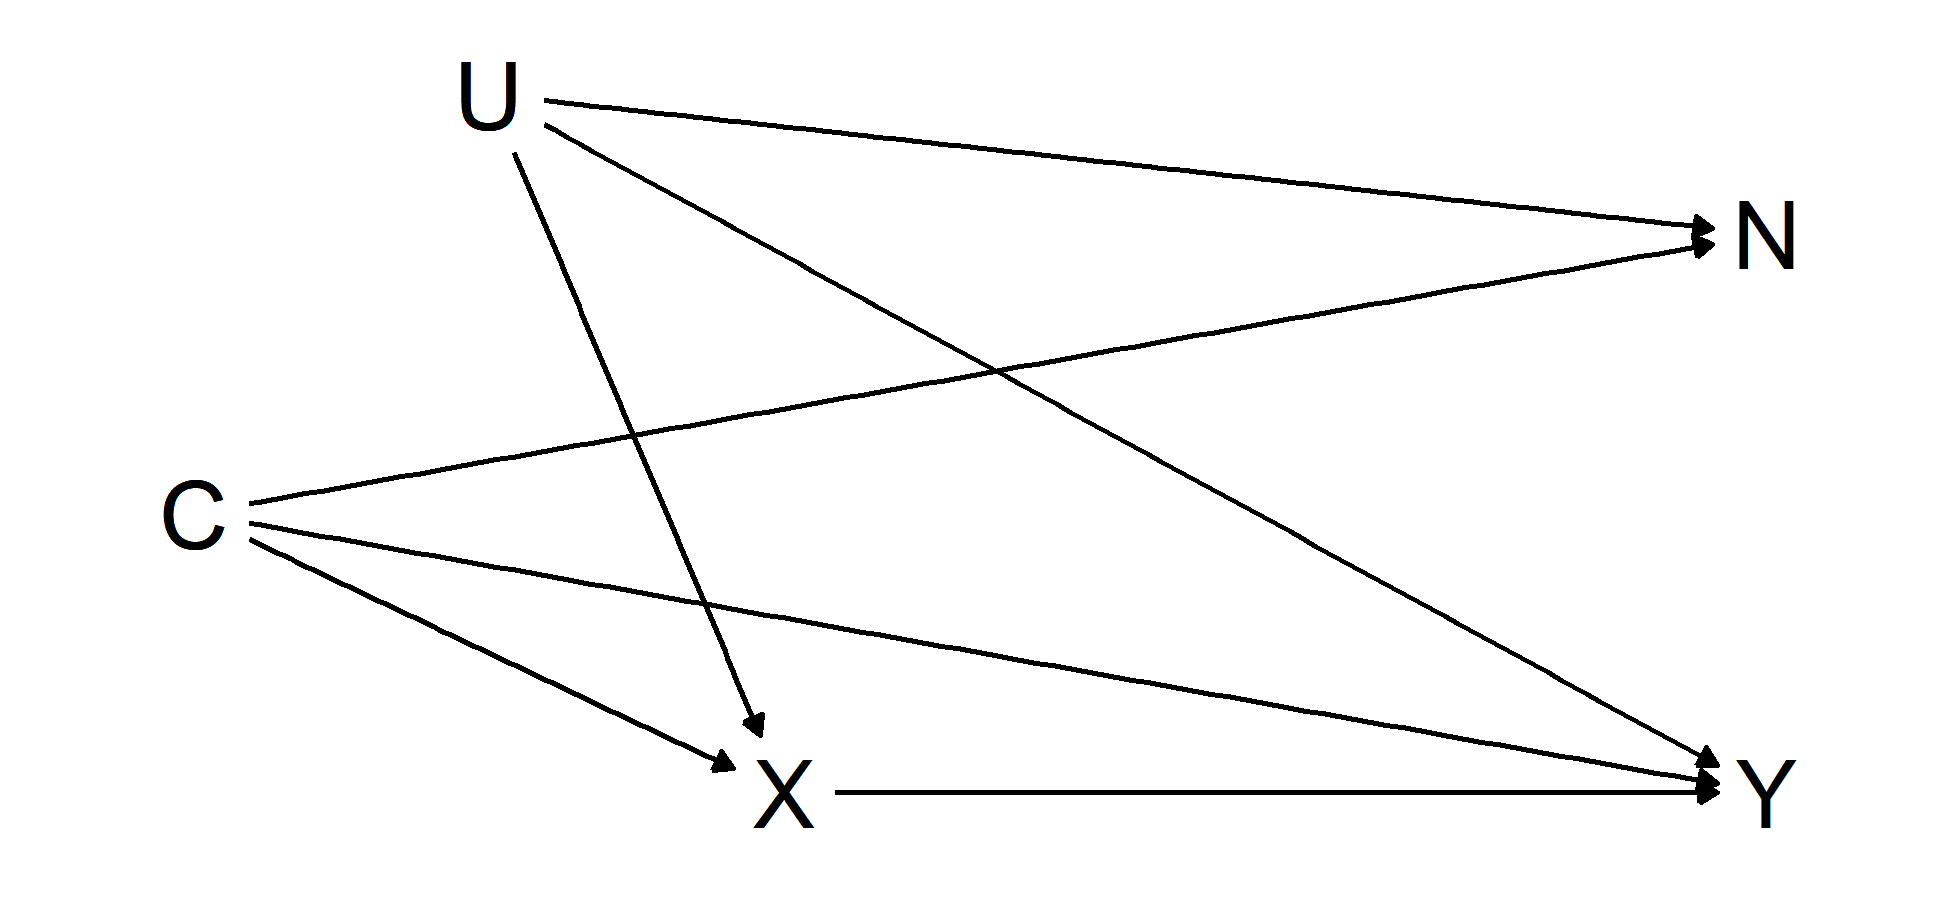
\includegraphics[width=0.8\linewidth]{figures/cprd-analysis/negativeOutcome} 

}

\caption[Causal diagram for ideal negative outcome]{Causal diagram (directed acyclic graph) showing relationship between exposure \(X\), outcome \(Y\), confounders (measured \(C\) and unmeasured \(U\)) and an ideal negative outcome \(N\). Note the absence of any arrow between \(X\) and \(N\). In this scenario, any association observed between \(X\) and \(N\) is due to the presence of uncontrolled confounders \(U\) (assuming \(C\) has been adjusted for).}\label{fig:negativeOutcome}
\end{figure}

~

Despite observational analyses suggesting a link between statins and muscular pain (as opposed to more serious complications such as myopathy),\textsuperscript{\protect\hyperlink{ref-selva-ocallaghan2018}{287}} systematic reviews of the adverse events of statin use\textsuperscript{\protect\hyperlink{ref-collins2016a}{30}} and N-of-1 trials explicitly exploring the association of statin use with muscle pain\textsuperscript{\protect\hyperlink{ref-herrett2021}{288}} have found little evidence supporting an effect. This suggests that muscular backpain would be suitable for use as a negative control outcome in this analysis. Under this approach, if statin use is found to be associated with muscular backpain in this analysis, this suggests the presence of residual confounding and reduces my confidence in the results for the dementia outcomes.

Similarly, incident ischemic heart disease and Type 2 diabetes were included as a protective and harmful positive control outcome, respectively. The protective effect of lipid-lowering treatment, via statins, on the risk of ischemic heart disease is well-established,\textsuperscript{\protect\hyperlink{ref-collins2016a}{30}} while there is growing evidence for an increased risk of Type 2 diabetes with statin use.\textsuperscript{\protect\hyperlink{ref-collins2016a}{30},\protect\hyperlink{ref-macedo2014}{289},\protect\hyperlink{ref-smit2020}{290}} Similar to the negative outcome, if the analysis strategy can reproduce these known associations, this will provide evidence that potential confounders have been sufficiently adjusted for.

~

\hypertarget{impact-of-additional-covariates}{%
\subsubsection{Impact of additional covariates}\label{impact-of-additional-covariates}}

To observe the effect of adjusting for additional covariates, I ran two additional models unadjusted except for: (a) age; and (b) age and gender. The results of these models was then compared the results with the fully adjusted model.

~

\hypertarget{sensitivity-cohorts}{%
\subsubsection{Sensitivity cohorts}\label{sensitivity-cohorts}}

Two sensitivity cohorts were also created. The first stratified by year of entry into the cohort in an attempt to assess for time period effects. The second removed participants who may have been pregnant (coded as under 55) to assess the robustness of the estimates, as statins are contraindicated in pregnancy.\textsuperscript{\protect\hyperlink{ref-karalis2016}{291}}

~

\hypertarget{statin-properties}{%
\subsubsection{Statin properties}\label{statin-properties}}

As detailed in the introduction, the properties of statins may be important in their effect based on the ability of lipophilic statins to cross the blood brain barrier (see Section \ref{intro-statins}).\textsuperscript{\protect\hyperlink{ref-sierra2011}{33}} To investigate this, I further stratified the statin exposure group into lipophilic (Atorvastatin, Lovastatin, Simvastatin, Cerivastatin) and hydrophilic (Pravastatin, Rosuvastatin, Fluvastatin) statins.

~

\hypertarget{comparing-dementia-codelists}{%
\subsubsection{Comparing dementia codelists}\label{comparing-dementia-codelists}}

As part of an exploratory analysis of the effect of the choice of code lists on the analysis, I created an alternative Alzheimer's disease and non-Alzheimer's dementia outcome using code lists from a published study by Smeeth \emph{et al}.\textsuperscript{\protect\hyperlink{ref-smeeth2009}{292}}

This previous analysis used a propensity matching approach to estimate the association of statins with a range of outcomes in The Health Improvement Network (THIN) database, a alternative source of English electronic health records which has substantial overlap with the CPRD.\textsuperscript{\protect\hyperlink{ref-carbonari2015}{293}} The code lists used in this analysis were obtained through correspondence with the authors of that study, and are available for inspection (see Section \ref{cprd-data-avail}).

~

\hypertarget{results-1}{%
\section{Results}\label{results-1}}

\hypertarget{patient-characteristics}{%
\subsection{Patient characteristics}\label{patient-characteristics}}

Of the 3,179,733 participants included in the extract, 1,684,564 met the inclusion criteria (Figure \ref{fig:cprdFlowchart}), with a total follow-up of 10,835,685 patient years at risk.

~





\begin{figure}[H]
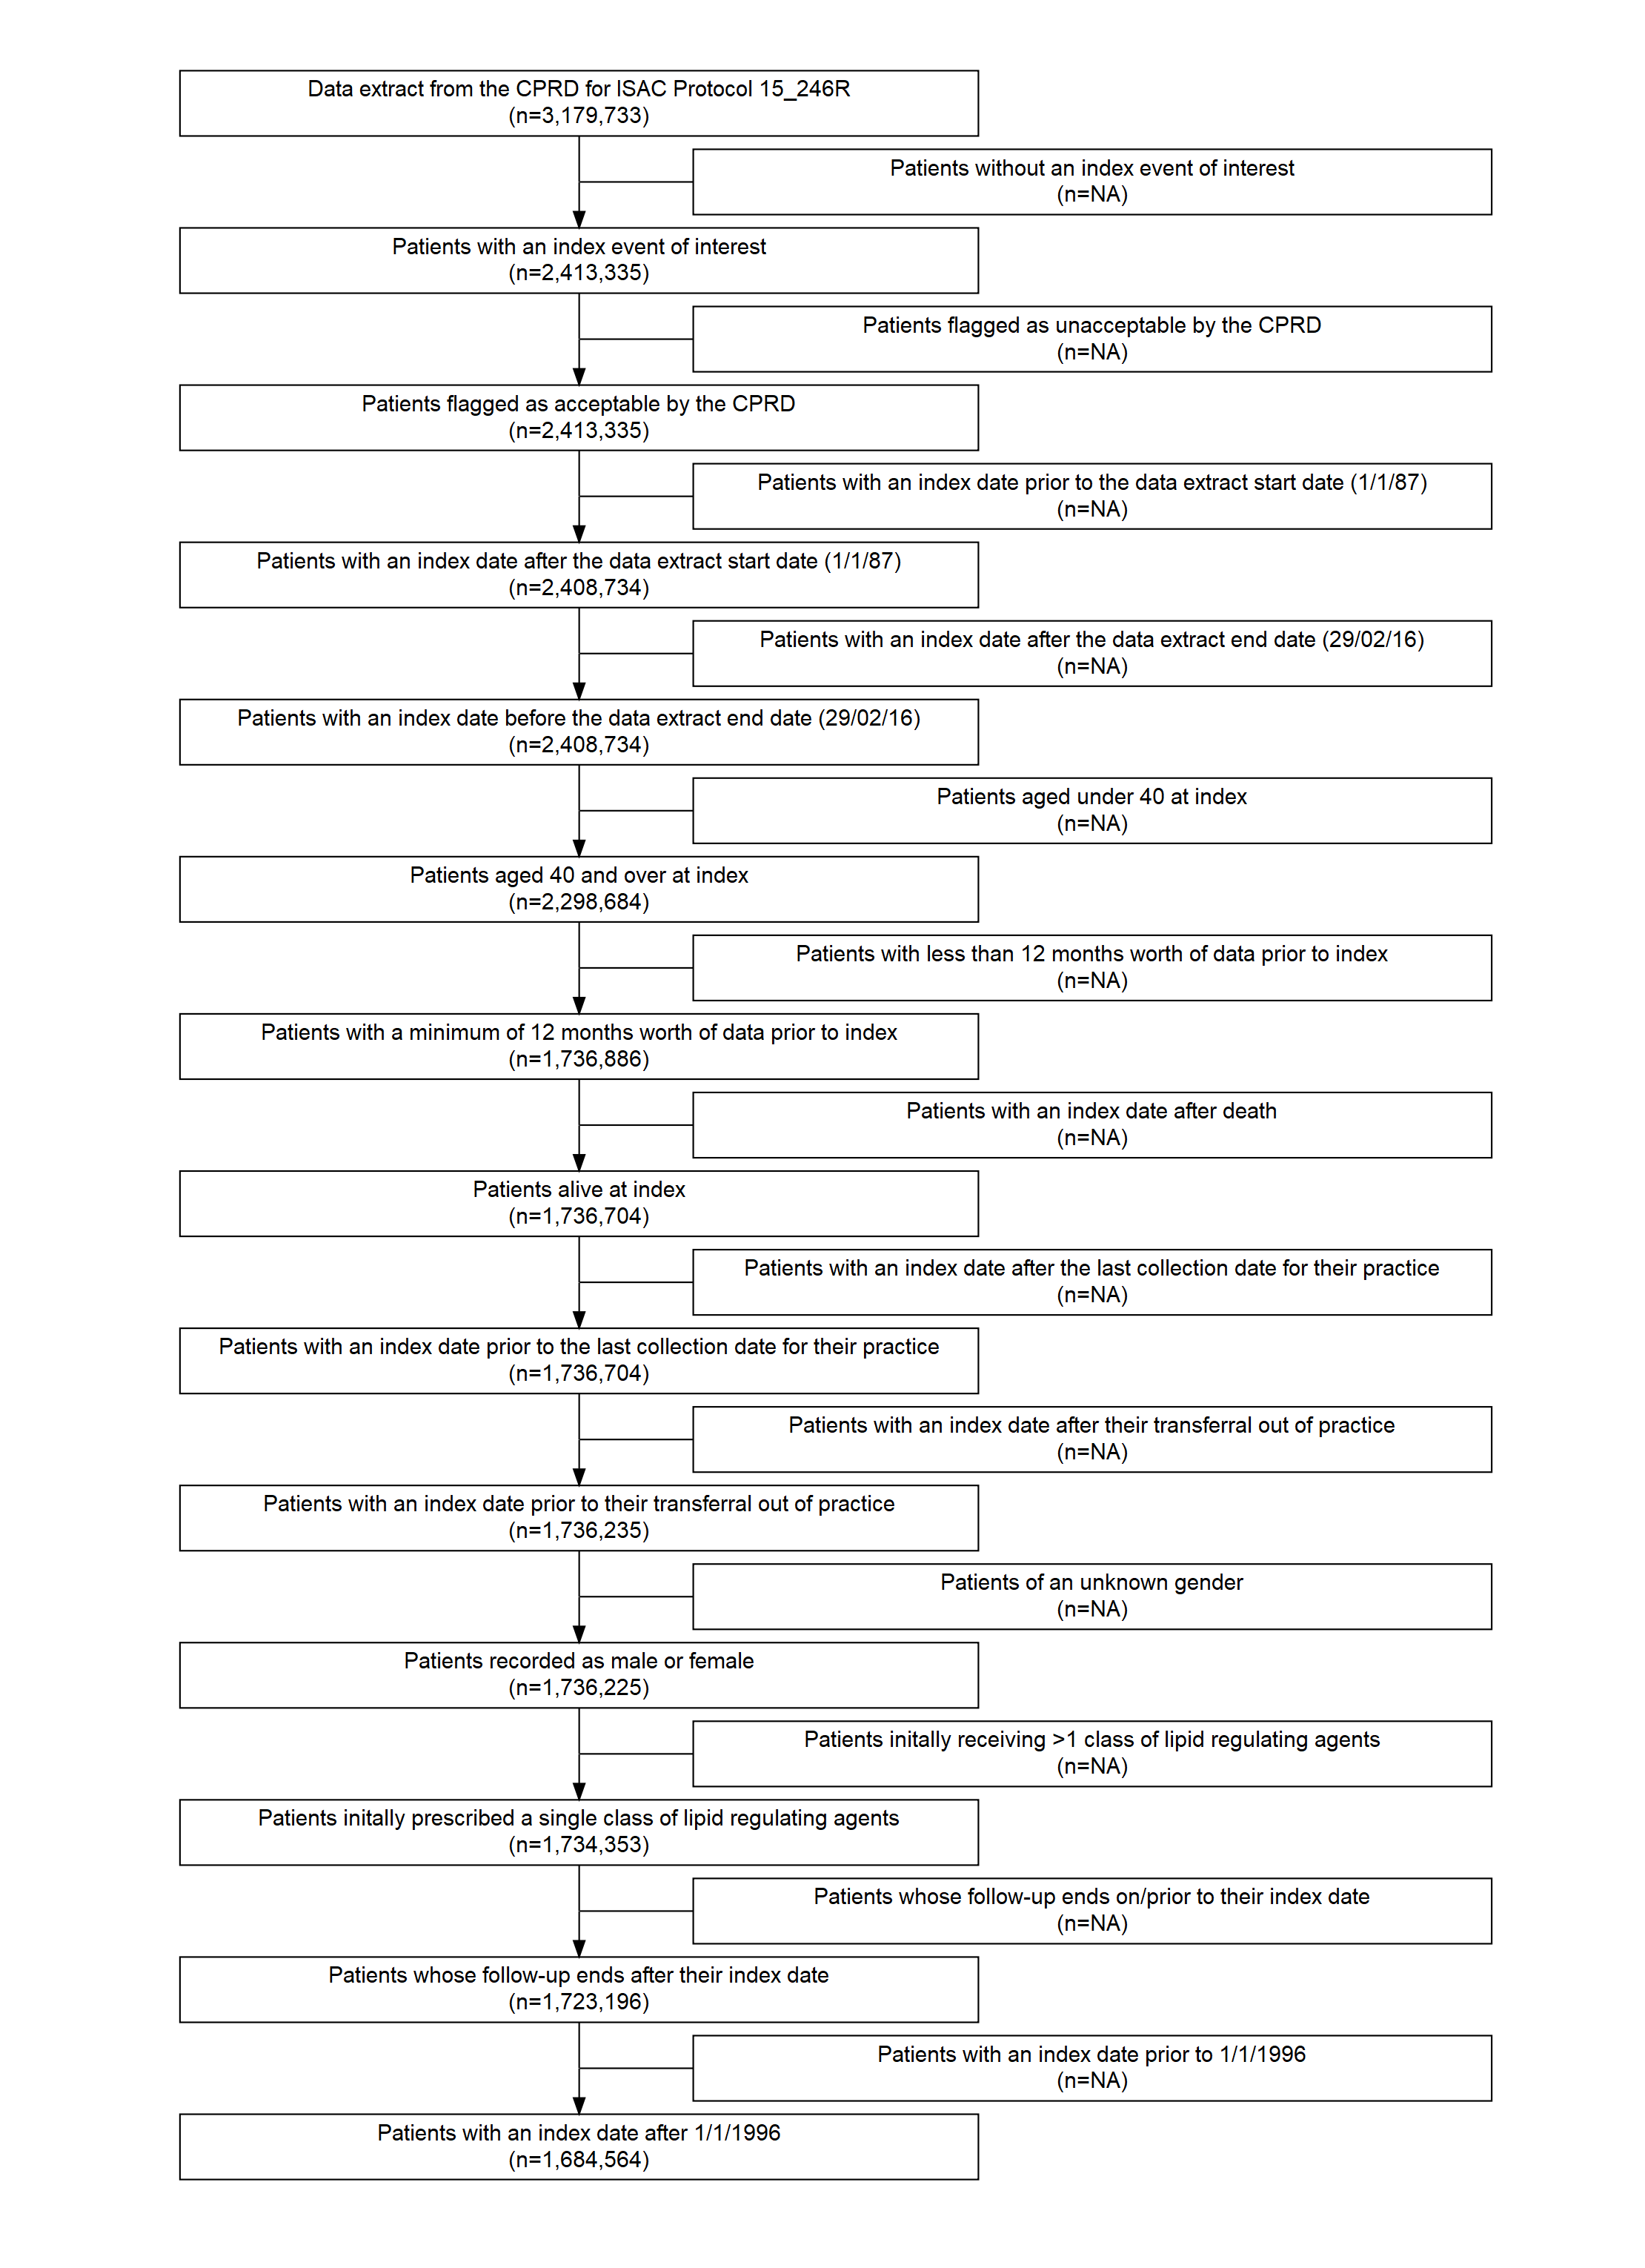
\includegraphics[width=1\linewidth]{figures/cprd-analysis/cohort_attrition} \caption[Attrition of CPRD participants]{Attrition of CPRD participants as the eligibility criteria were applied. The largest cause of attrition was the absence of an index event of interest.}\label{fig:cprdFlowchart}
\end{figure}

~

The median participant age at index was 57 years (inter-quartile range (IQR):48-67) and participants were followed up for a median of 5.9 years (IQR:2.7-9.7). During follow-up, an all-cause dementia diagnosis was recorded for 41,830 patients (12,647 probable AD, 9,954 possible AD, 8,466 vascular dementia, 10,763 other dementias).

The number of events, time-at-risk and crude rates for each drug class, tabulated by dementia outcome, are shown in Table \ref{tab:followUp-table}. A substantial majority (98.1\%) of participants prescribed a lipid-regulating agent were prescribed a statin. I excluded the ``Ezetimibe and statins'' (n=127) and ``Nicotinic acid groups'' (n= 165) classes from subsequent class-based subgroup analyses based on the extremely small number of participants in these groups. Note that the ``Ezetimibe and statins'' treatment group represent those prescribed a single treatment containing both ezetimibe and statins, rather than those where the two treatments were prescribed concurrently.

\blandscape





\begin{table}

\caption[Crude rates, stratified by outcome and drug class of interest.]{\label{tab:followUp-table}Summary of number of events, years at risk and crude rates per 100,000 participant-years-at-risk stratified by dementia outcome and drug class of interest.}
\centering
\fontsize{8}{10}\selectfont
\begin{threeparttable}
\begin{tabular}[t]{>{}l|>{\centering\arraybackslash}p{3em}>{\centering\arraybackslash}p{3em}>{}c|>{\centering\arraybackslash}p{3em}>{\centering\arraybackslash}p{3em}>{}c|>{\centering\arraybackslash}p{3em}>{\centering\arraybackslash}p{3em}>{}c|>{\centering\arraybackslash}p{3em}>{\centering\arraybackslash}p{3em}>{}c|>{\centering\arraybackslash}p{3em}>{\centering\arraybackslash}p{3em}>{\centering\arraybackslash}p{3em}}
\toprule
\multicolumn{1}{c}{\textbf{ }} & \multicolumn{3}{c}{\textbf{Any dementia}} & \multicolumn{3}{c}{\textbf{Possible AD}} & \multicolumn{3}{c}{\textbf{Probable AD}} & \multicolumn{3}{c}{\textbf{Vascular dementia}} & \multicolumn{3}{c}{\textbf{Other dementia}} \\
\cmidrule(l{3pt}r{3pt}){2-4} \cmidrule(l{3pt}r{3pt}){5-7} \cmidrule(l{3pt}r{3pt}){8-10} \cmidrule(l{3pt}r{3pt}){11-13} \cmidrule(l{3pt}r{3pt}){14-16}
\textbf{Exposure Group} & \textbf{Events} & \textbf{PYAR} & \textbf{Rate \textsuperscript{*}} & \textbf{Events} & \textbf{PYAR} & \textbf{Rate \textsuperscript{*}} & \textbf{Events} & \textbf{PYAR} & \textbf{Rate \textsuperscript{*}} & \textbf{Events} & \textbf{PYAR} & \textbf{Rate \textsuperscript{*}} & \textbf{Events} & \textbf{PYAR} & \textbf{Rate \textsuperscript{*}}\\
\midrule
\textbf{No LRA (unexposed)} & 18,608 & 5,872,717 & 317 & 6,368 & 5,818,047 & 109 & 2,637 & 5,800,964 & 45 & 4,813 & 5,811,594 & 83 & 4,790 & 5,808,285 & 82\\
\textbf{By drug class} &  &  &  &  &  &  &  &  &  &  &  &  &  &  & \\
\hspace{1em}Statins & 22,920 & 4,871,568 & 470 & 6,190 & 4,758,526 & 130 & 5,773 & 4,753,437 & 121 & 5,871 & 4,755,258 & 123 & 5,086 & 4,747,237 & 107\\
\hspace{1em}Omega-3 FAGs & 19 & 8,034 & 236 & 4 & 7,927 & 50 & 7 & 7,950 & 88 & 4 & 7,938 & 50 & 4 & 7,925 & 50\\
\hspace{1em}Fibrates & 141 & 38,003 & 371 & 49 & 37,102 & 132 & 21 & 36,835 & 57 & 36 & 37,001 & 97 & 35 & 36,983 & 95\\
\hspace{1em}Ezetimibe & 32 & 6,604 & 485 & 8 & 6,429 & 124 & 7 & 6,425 & 109 & 12 & 6,444 & 186 & 5 & 6,393 & 78\\
\hspace{1em}BAS & 106 & 36,370 & 291 & 28 & 35,808 & 78 & 19 & 35,726 & 53 & 26 & 35,768 & 73 & 33 & 35,808 & 92\\
\hspace{1em}Ezetimibe + Statins \textsuperscript{\dag} & 0 & 986 & - & 0 & 986 & - & 0 & 986 & - & 0 & 986 & - & 0 & 986 & -\\
\hspace{1em}NAG & 4 & 1,403 & - & 0 & 1,379 & - & 2 & 1,391 & - & 1 & 1,389 & - & 1 & 1,382 & -\\
\midrule
\textbf{Total} & 41,830 & 10,835,686 & 386 & 12,647 & 10,666,205 & 119 & 8,466 & 10,643,714 & 80 & 10,763 & 10,656,378 & 101 & 9,954 & 10,644,999 & 94\\
\bottomrule
\end{tabular}
\begin{tablenotes}
\item \textsuperscript{*} Crude rate per 100,000 participant-years-at-risk\newline \textsuperscript{\dag} One treatment containing both drugs, rather than the two classes being prescribed concurrently\newline \textbf{Abbreviations:} AD - Alzheimer's disease;  BAS - Bile acid sequestrants; LRA - Lipid regulating agent;  NAG - Nicotinic acid groups;  Omega-3 FGs - Omega-3 Fatty acid groups; PYAR - Participant-years-at-risk.
\end{tablenotes}
\end{threeparttable}
\end{table}





\begin{table}[H]

\caption[Patient characteristics by drug class]{\label{tab:cprdCharacteristics-table}Patient characteristics by drug class. Summary statistics are presented as ``\% (N)'' unless otherwise specified in the variable name.}
\centering
\fontsize{7}{9}\selectfont
\begin{threeparttable}
\begin{tabular}[t]{>{\raggedright\arraybackslash}p{15em}>{\centering\arraybackslash}p{7.7em}>{\centering\arraybackslash}p{7.7em}>{\centering\arraybackslash}p{7.7em}>{\centering\arraybackslash}p{7.7em}>{\centering\arraybackslash}p{7.7em}>{\centering\arraybackslash}p{7.7em}>{\centering\arraybackslash}p{7.7em}}
\toprule
\textbf{ } & \textbf{Whole Sample} & \textbf{None} & \textbf{Statins} & \textbf{Bile acid sequestrants} & \textbf{Ezetimibe} & \textbf{Fibrates} & \textbf{Omega-3 Fatty Acid Groups}\\
\midrule
\textbf{Sample size (N)} & 1,684,564 & 1,087,704 & 585,528 & 5,396 & 763 & 3,889 & 992\\
\midrule
\textbf{Year of cohort entry \newline (median)} & 2006 & 2007 & 2004 & 2005 & 2004 & 2001 & 2005\\
\midrule
\textbf{Female} & 53.0\% (893174) & 56.2\% (610950) & 47.1\% (276043) & 66.4\% (3585) & 54.5\% (416) & 38.6\% (1500) & 52.6\% (522)\\
\midrule
\textbf{Age at cohort entry \newline (median)} & 57 & 54 & 62 & 57 & 60 & 58 & 56\\
\midrule
\textbf{CAD} & 0.4\% (7133) & 0.1\% (589) & 1.1\% (6465) & 0.1\% (6) & 0.9\% (7) & 1.4\% (53) & 1.3\% (13)\\
\midrule
\addlinespace
\textbf{CBS} & 0.3\% (5699) & 0.1\% (682) & 0.8\% (4926) & 0.1\% (4) & 0.4\% (3) & 2.0\% (78) & 0.6\% (6)\\
\midrule
\textbf{CVD} & 2.1\% (34899) & 1.1\% (11619) & 3.9\% (22977) & 1.6\% (86) & 2.6\% (20) & 4.4\% (170) & 1.7\% (17)\\
\midrule
\textbf{Charlson (ever > 0)} & 30.6\% (516135) & 25.1\% (272642) & 40.7\% (238403) & 42.5\% (2292) & 41.7\% (318) & 50.8\% (1976) & 40.4\% (401)\\
\midrule
\textbf{IMD-2010 (median)} & 9 & 8 & 9 & 8 & 9 & 10 & 10\\
\midrule
\textbf{Consultation rate (mean/SD)} & 5.4 (5.4) & 5.0 (5.0) & 6.2 (6.1) & 8.6 (7.4) & 7.4 (6.6) & 7.1 (6.2) & 8.0 (8.0)\\
\midrule
\addlinespace
\textbf{Alcohol (ever)} & 85.9\% (1447151) & 86.6\% (941648) & 84.7\% (496110) & 82.8\% (4468) & 84.0\% (641) & 82.9\% (3223) & 82.0\% (813)\\
\midrule
\textbf{Smoking (ever)} & 51.1\% (861355) & 47.1\% (511826) & 58.6\% (343074) & 55.2\% (2978) & 57.5\% (439) & 60.2\% (2341) & 53.7\% (533)\\
\midrule
\textbf{BMI (mean/SD)} & 27.0 (5.3) & 26.7 (5.2) & 27.7 (5.3) & 26.8 (5.8) & 28.1 (5.7) & 29.0 (5.2) & 26.9 (5.5)\\
\midrule
\textbf{PAD} & 0.7\% (12613) & 0.4\% (4039) & 1.4\% (8424) & 0.9\% (47) & 0.9\% (7) & 1.9\% (75) & 1.0\% (10)\\
\midrule
\textbf{Hypertension} & 16.0\% (269804) & 11.5\% (124604) & 24.4\% (143101) & 12.8\% (692) & 23.9\% (182) & 25.8\% (1002) & 15.7\% (156)\\
\midrule
\addlinespace
\textbf{Total cholesterol (mean/SD)} & 5.7 (10.1) & 5.5 (6.4) & 6.2 (15.3) & 5.3 (1.3) & 7.1 (26.5) & 6.4 (5.6) & 5.6 (1.6)\\
\midrule
\textbf{LDL cholesterol (mean/SD)} & 3.6 (4.9) & 3.4 (5.3) & 4.0 (3.7) & 3.1 (1.0) & 3.9 (1.1) & 3.3 (1.8) & 3.2 (1.0)\\
\midrule
\textbf{CKD} & 0.1\% (1295) & 0.1\% (740) & 0.1\% (545) & 0.1\% (6) & 0.1\% (1) & 0.0\% (0) & 0.3\% (3)\\
\midrule
\textbf{Type 1 Diabetes} & 0.2\% (4037) & 0.1\% (785) & 0.5\% (3196) & 0.3\% (14) & 1.0\% (8) & 0.8\% (31) & 0.1\% (1)\\
\midrule
\textbf{Type 2 Diabetes} & 2.9\% (48557) & 1.1\% (11797) & 6.1\% (35941) & 2.3\% (123) & 5.4\% (41) & 15.8\% (614) & 2.8\% (28)\\
\bottomrule
\end{tabular}
\begin{tablenotes}
\item \textit{Note:} The 'Nicotinic acid groups' (n=165) and 'Ezetimibe and Statins' (n=127) subgroups are not shown, but are included in the whole sample column\newline \textbf{Abbreviations:} BMI - Body mass index; CAD - Coronary arterial disease; CBS - Coronary bypass surgery; CKD - Chronic kidney disease; CVD - Cardiovascular disease; IMD - Index of multiple deprivation; LRA - Lipid regulating agent; PAD - Peripheral arterial disease; SD - Standard deviation.
\end{tablenotes}
\end{threeparttable}
\end{table}

\elandscape

The distribution of baseline characteristics across the remaining seven drug classes can be seen in Table \ref{tab:cprdCharacteristics-table}. Note due to the experimental design, the median year of entry is expected to be later for those not prescribed an LRA, as this exposure group is more likely to include those who entered into the cohort towards the end of study window (as these people had less follow-up time in which to be prescribed an LRA).

The stopping, addition and switching of drug classes was common across all drug classes (Table \ref{tab:cprdSSA-table}).

~\\




\begin{table}[H]

\caption[Participants who stopped, switched or added treatements by initial treatment type]{\label{tab:cprdSSA-table}Participants who stopped, switched or added treatments by initial treatment type.}
\centering
\fontsize{7}{9}\selectfont
\begin{threeparttable}
\begin{tabular}[t]{>{\raggedright\arraybackslash}p{5em}>{\centering\arraybackslash}p{4.225em}>{\centering\arraybackslash}p{4.225em}>{\centering\arraybackslash}p{4.225em}>{\centering\arraybackslash}p{4.225em}>{\centering\arraybackslash}p{4.225em}>{\centering\arraybackslash}p{4.225em}>{\centering\arraybackslash}p{4.225em}>{\centering\arraybackslash}p{4.225em}}
\toprule
\textbf{ } & \textbf{Whole Sample} & \textbf{Statins} & \textbf{Bile acid sequestrants} & \textbf{Ezetimibe} & \textbf{Ezetimibe \& Statins} & \textbf{Fibrates} & \textbf{Nicotinic acid groups} & \textbf{Omega-3 Fatty Acid Groups}\\
\midrule
\textbf{Stopped} & 6.9\% (115899) & 19.1\% (111798) & 56.1\% (3028) & 19.7\% (150) & 12.6\% (16) & 12.3\% (478) & 44.8\% (74) & 35.8\% (355)\\
\midrule
\textbf{Added} & 1.6\% (27441) & 4.4\% (25990) & 3.6\% (192) & 19.0\% (145) & 3.9\% (5) & 21.6\% (841) & 3.6\% (6) & 26.4\% (262)\\
\midrule
\textbf{Switched} & 0.9\% (14935) & 2.0\% (11996) & 11.3\% (612) & 34.6\% (264) & 64.6\% (82) & 44.0\% (1713) & 45.5\% (75) & 19.5\% (193)\\
\bottomrule
\end{tabular}
\begin{tablenotes}
\item \textbf{Defintions:} Stopped - last prescription of the primary drug class followed by at least six months of observation with no further prescriptions; Added - second drug class prescribed before the last prescription of the initial class; Switched - second drug class being prescribed after the last prescription of the initial class.
\end{tablenotes}
\end{threeparttable}
\end{table}

~

\hypertarget{missing-data-1}{%
\subsection{Missing data}\label{missing-data-1}}

Full covariate information was available for 450,234 participants (26.7\%). Six key variables had some missing data: IMD 2010 score was missing for 625,788 participants (37.1\%), because it is only recorded for English practices; alcohol status was missing for 269,526 participants (16\%); smoking status was missing for 84,424 participants (5\%); BMI, or a calculated BMI from height and weight measurements, was missing for 266,672 participants (15.8\%); baseline total cholesterol was missing for 119,675 participants (7.1\%); and baseline LDL cholesterol was missing for 787,289 participants (46.7\%).

~

\hypertarget{primary-analysis}{%
\subsection{Primary analysis}\label{primary-analysis}}

The results of the primary analysis using the fully adjusted Cox proportional hazards model with participant age as the time scale are presented for each drug/outcome combination in Figure \ref{fig:cprdPrimary}.

For each outcome, the overall ``Any drug'' estimate was driven by the statin subgroup, based on its large size relative to the other drug classes.

~





\begin{figure}[H]
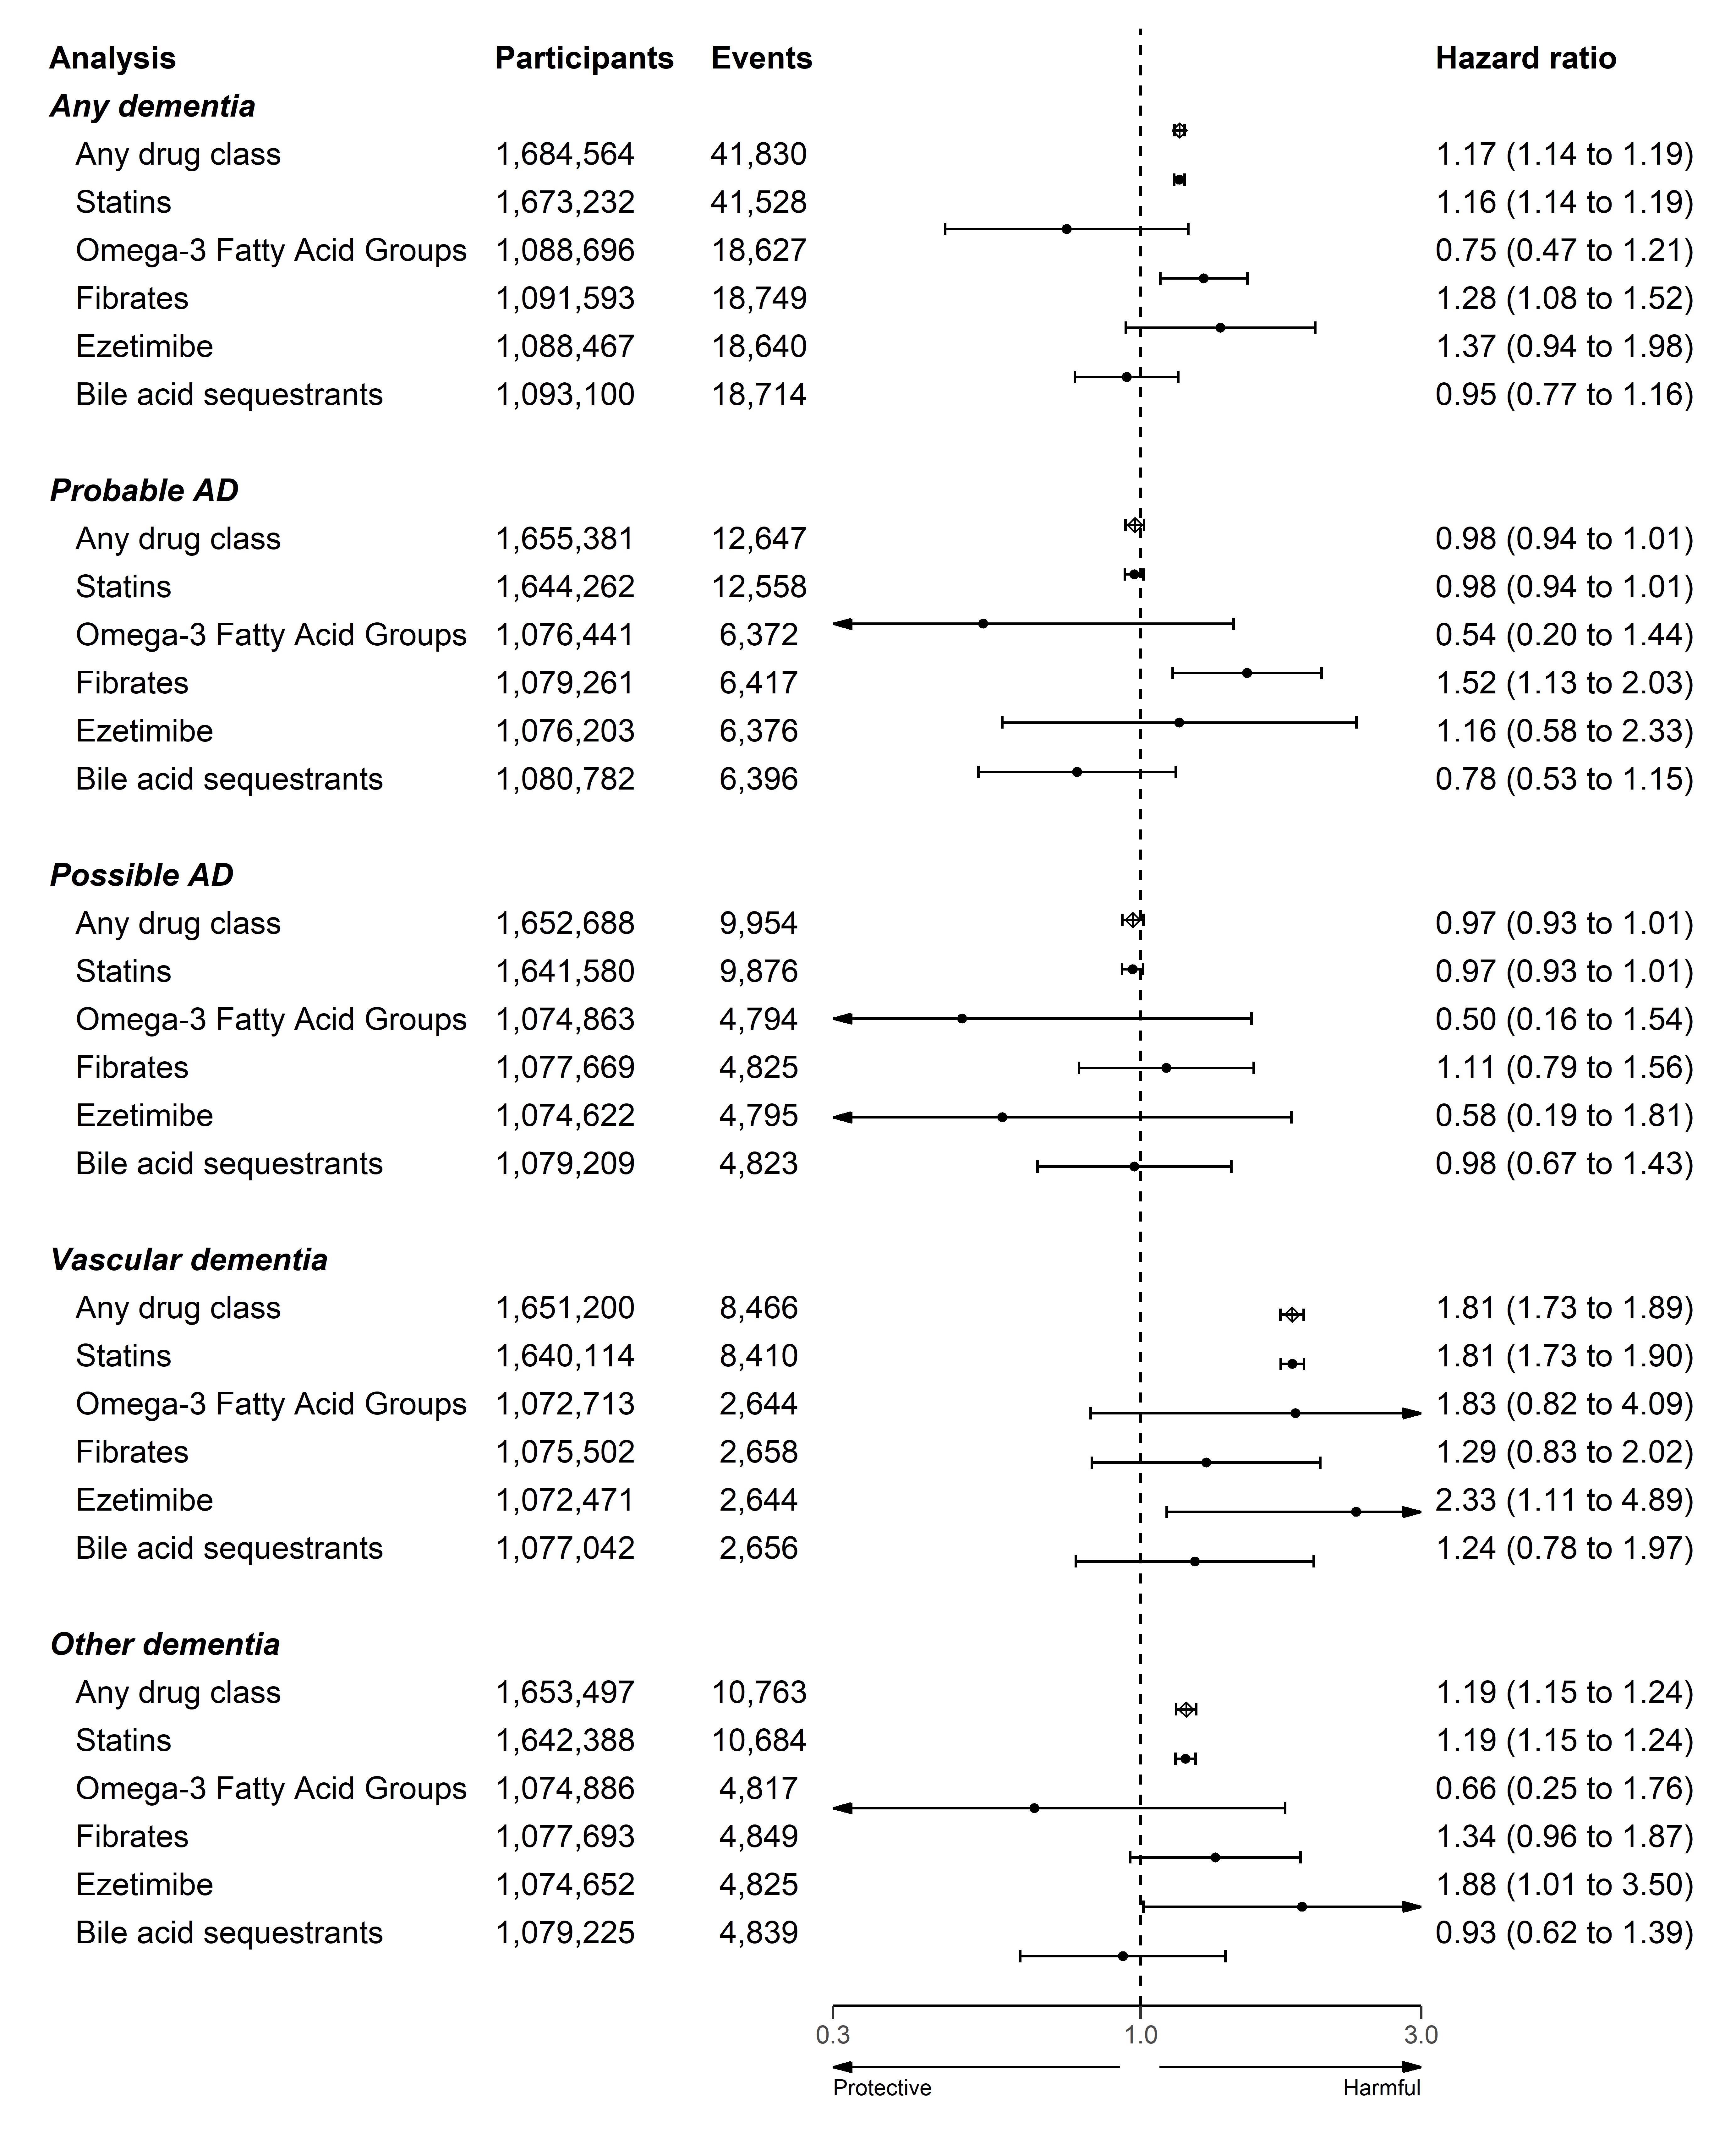
\includegraphics[width=1\linewidth]{figures/cprd-analysis/forester_p1} \caption[Results from primary analyses of CPRD data]{Results from primary analyses of CPRD data using the fully adjusted model and participant age as the time scale.}\label{fig:cprdPrimary}
\end{figure}

~

\textbf{Alzheimer's disease}

My results show litte evidence was found for an effect of lipid-regulating agents on probable (HR:0.98, 95\%CI:0.94-1.01) and possible (HR:0.97, 95\%CI:0.93-1.01) Alzheimer's disease when compared to no treatment, with the sole exception of fibrates on probable Alzheimer's disease (HR:1.52, 95\%CI:1.13-2.03).

~

\textbf{Non-Alzheimer's disease dementias}

In contrast to the findings for Alzheimer's disease outcomes, lipid-regulating agents were associated with an increased risk of a subsequent diagnosis of vascular dementia (HR:1.81, 95\%CI:1.73-1.89) or other dementias (HR:1.19, 95\%CI:1.15-1.24). Again this effect was driven mainly by the statin subgroup, but there was some evidence that ezetimibe was associated with an increased risk of vascular (HR:2.33, 95\%CI:1.11-4.89) and other (HR:1.88, 95\%CI:1.01-3.5) dementia.

~

\textbf{All-cause dementia}

For the composite all-cause dementia outcome, we found treatment with a lipid-regulating agent was associated with a slightly increased risk (HR:1.17, 95\%CI:1.14-1.19), which lies between the associations for the Alzheimer and non-Alzheimer dementia outcomes as would be expected. There was also some evidence that fibrates were associated with increased risk of all-cause dementia (HR:1.28, 95\%CI:1.08-1.52).

~

\hypertarget{sensitivity-analyses-1}{%
\subsection{Sensitivity analyses}\label{sensitivity-analyses-1}}

The results of the series of sensitivity analyses performed are described in the following sections.

\hypertarget{complete-case-versus-imputed-data}{%
\subsubsection{Complete case versus imputed data}\label{complete-case-versus-imputed-data}}

In almost all cases, the use of imputed data resulted in a marginal attenuation of the effects observed when using a complete cases analysis. It should be noted that due to the large amount of missing data (e.g.~787,289 participants (46.7\%) were missing a baseline LDL cholesterol measure), the number of participants included in the complete case analysis was substantially smaller than that included when using imputed data. In this case, though the overall position of the effect estimates does not change substantially when using the imputed dataset, there is a noticeable gain in power.\textsuperscript{\protect\hyperlink{ref-sterne2009}{278}}

~





\begin{figure}[H]
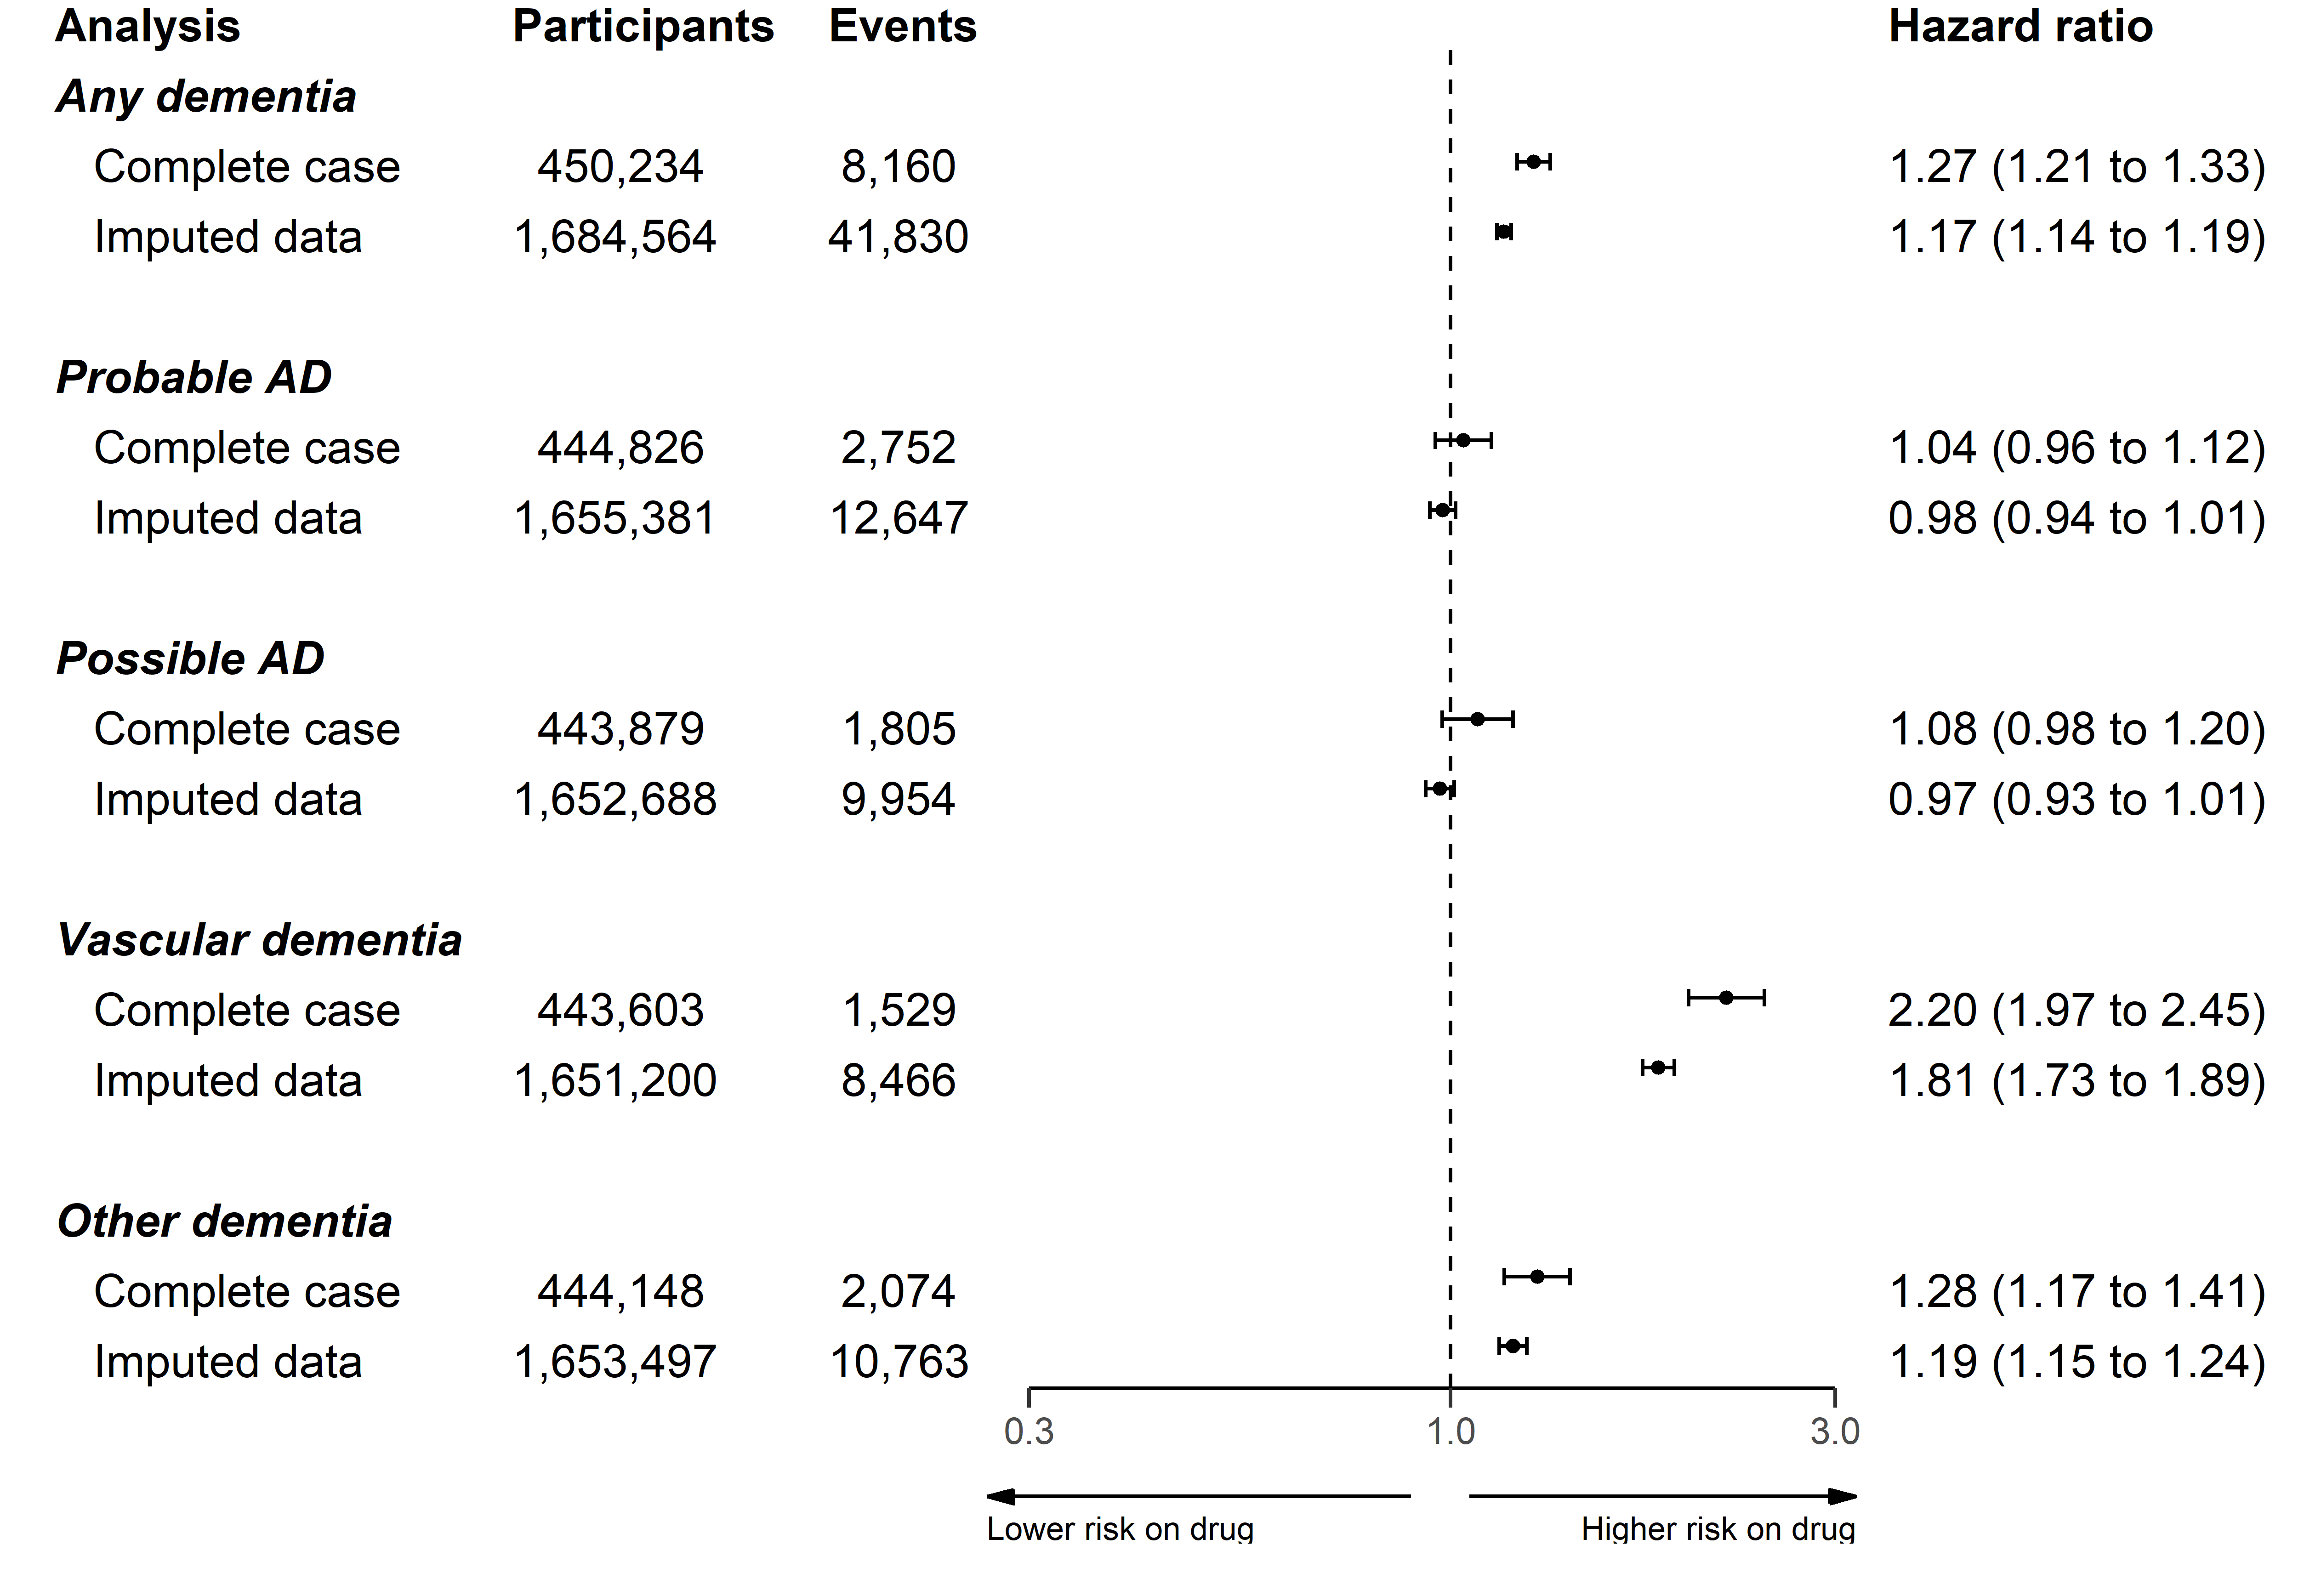
\includegraphics[width=1\linewidth]{figures/cprd-analysis/forester_complete_case} \caption[Complete case vs.~imputed data analysis]{Comparison of analyses using the complete case versus imputed cohorts.}\label{fig:completeCaseFig}
\end{figure}

~

\hypertarget{control-outcomes-1}{%
\subsubsection{Control outcomes}\label{control-outcomes-1}}

Following the primary analysis, the fully adjusted model was used to estimate the effect of treatment with a statin on the two control outcomes of back pain (negative) and ischemic heart disease (positive). The results of this analysis are presented in Figure \ref{fig:controlOutcomeFig}.

For the negative control, there was some evidence that treatment with a statin was associated with an increased risk of back pain (HR: 1.04, 95\%CI: 1.03-1.05), suggesting there may be some residual confounding. However, statin prescription was also associated with a substantially increased risk of ischemic heart disease (HR: 1.62, 95\%CI: 1.59-1.64) and Type 2 diabetes (HR: 1.50, 95\%CI: 1.48-1.51).

~





\begin{figure}[H]
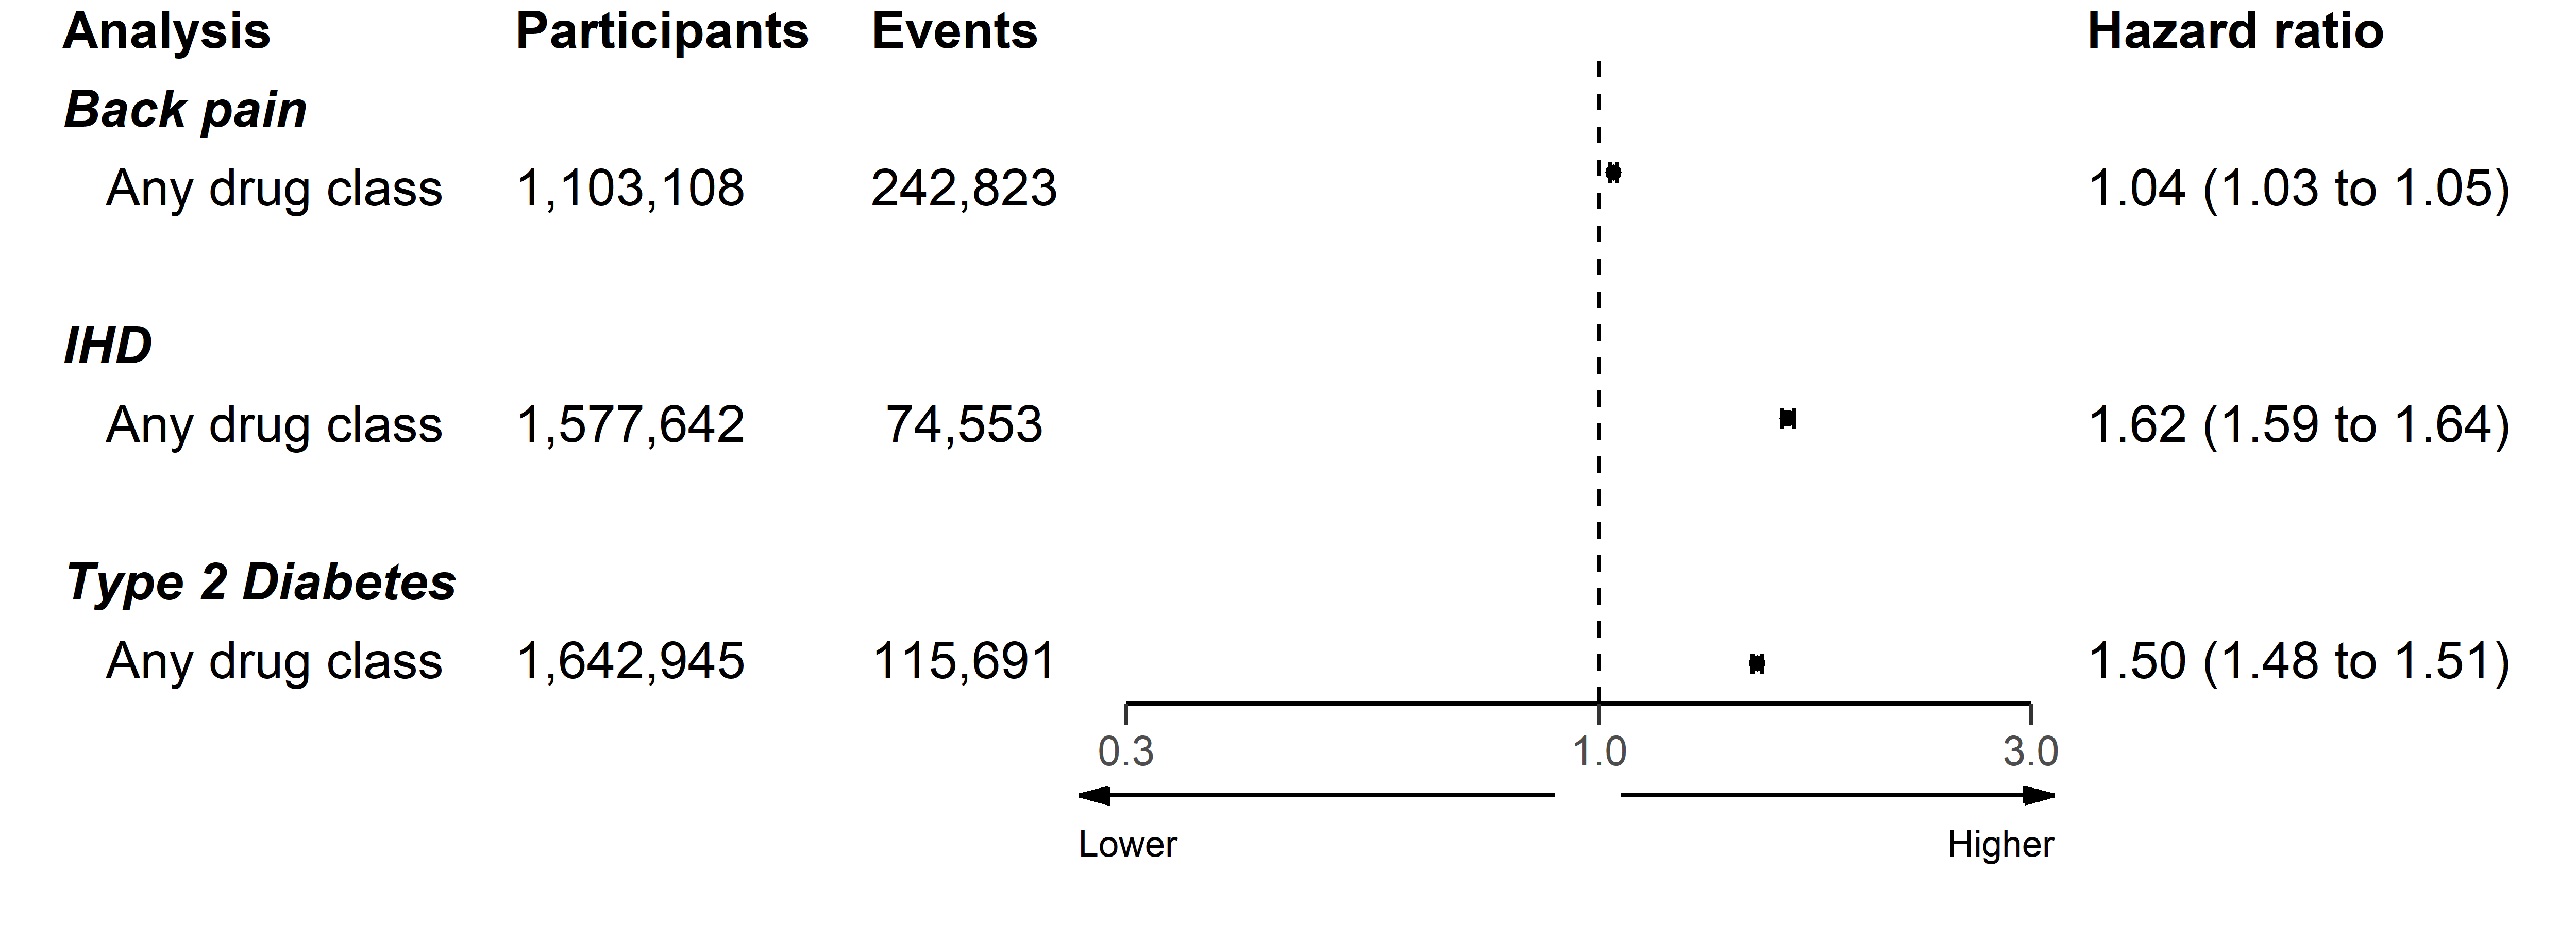
\includegraphics[width=1\linewidth]{figures/cprd-analysis/forester_control_outcomes} \caption[Results of control outcome analysis]{Results of control outcome analysis.}\label{fig:controlOutcomeFig}
\end{figure}

~

\hypertarget{impact-of-additional-covariates-1}{%
\subsubsection{Impact of additional covariates}\label{impact-of-additional-covariates-1}}

The results of three models adjusted for age only, age and sex, and the full covariates respectively, are presented in Figure \ref{fig:unadjustedComparisonFig}. These models were used to estimate the impact of adjustment for additional covariates. Note that obtaining an completely unadjusted model is not possible, as age was used in the Cox model as the time scale.

Adjustment for additional covariates beyond age and sex had a limited impact on the observed effect estimates, with the exception of the probable AD outcome. In this case, adjustment for the full set of covariates attenuated to the null the protective effect observed when adjusting only for age and sex.

~





\begin{figure}[H]
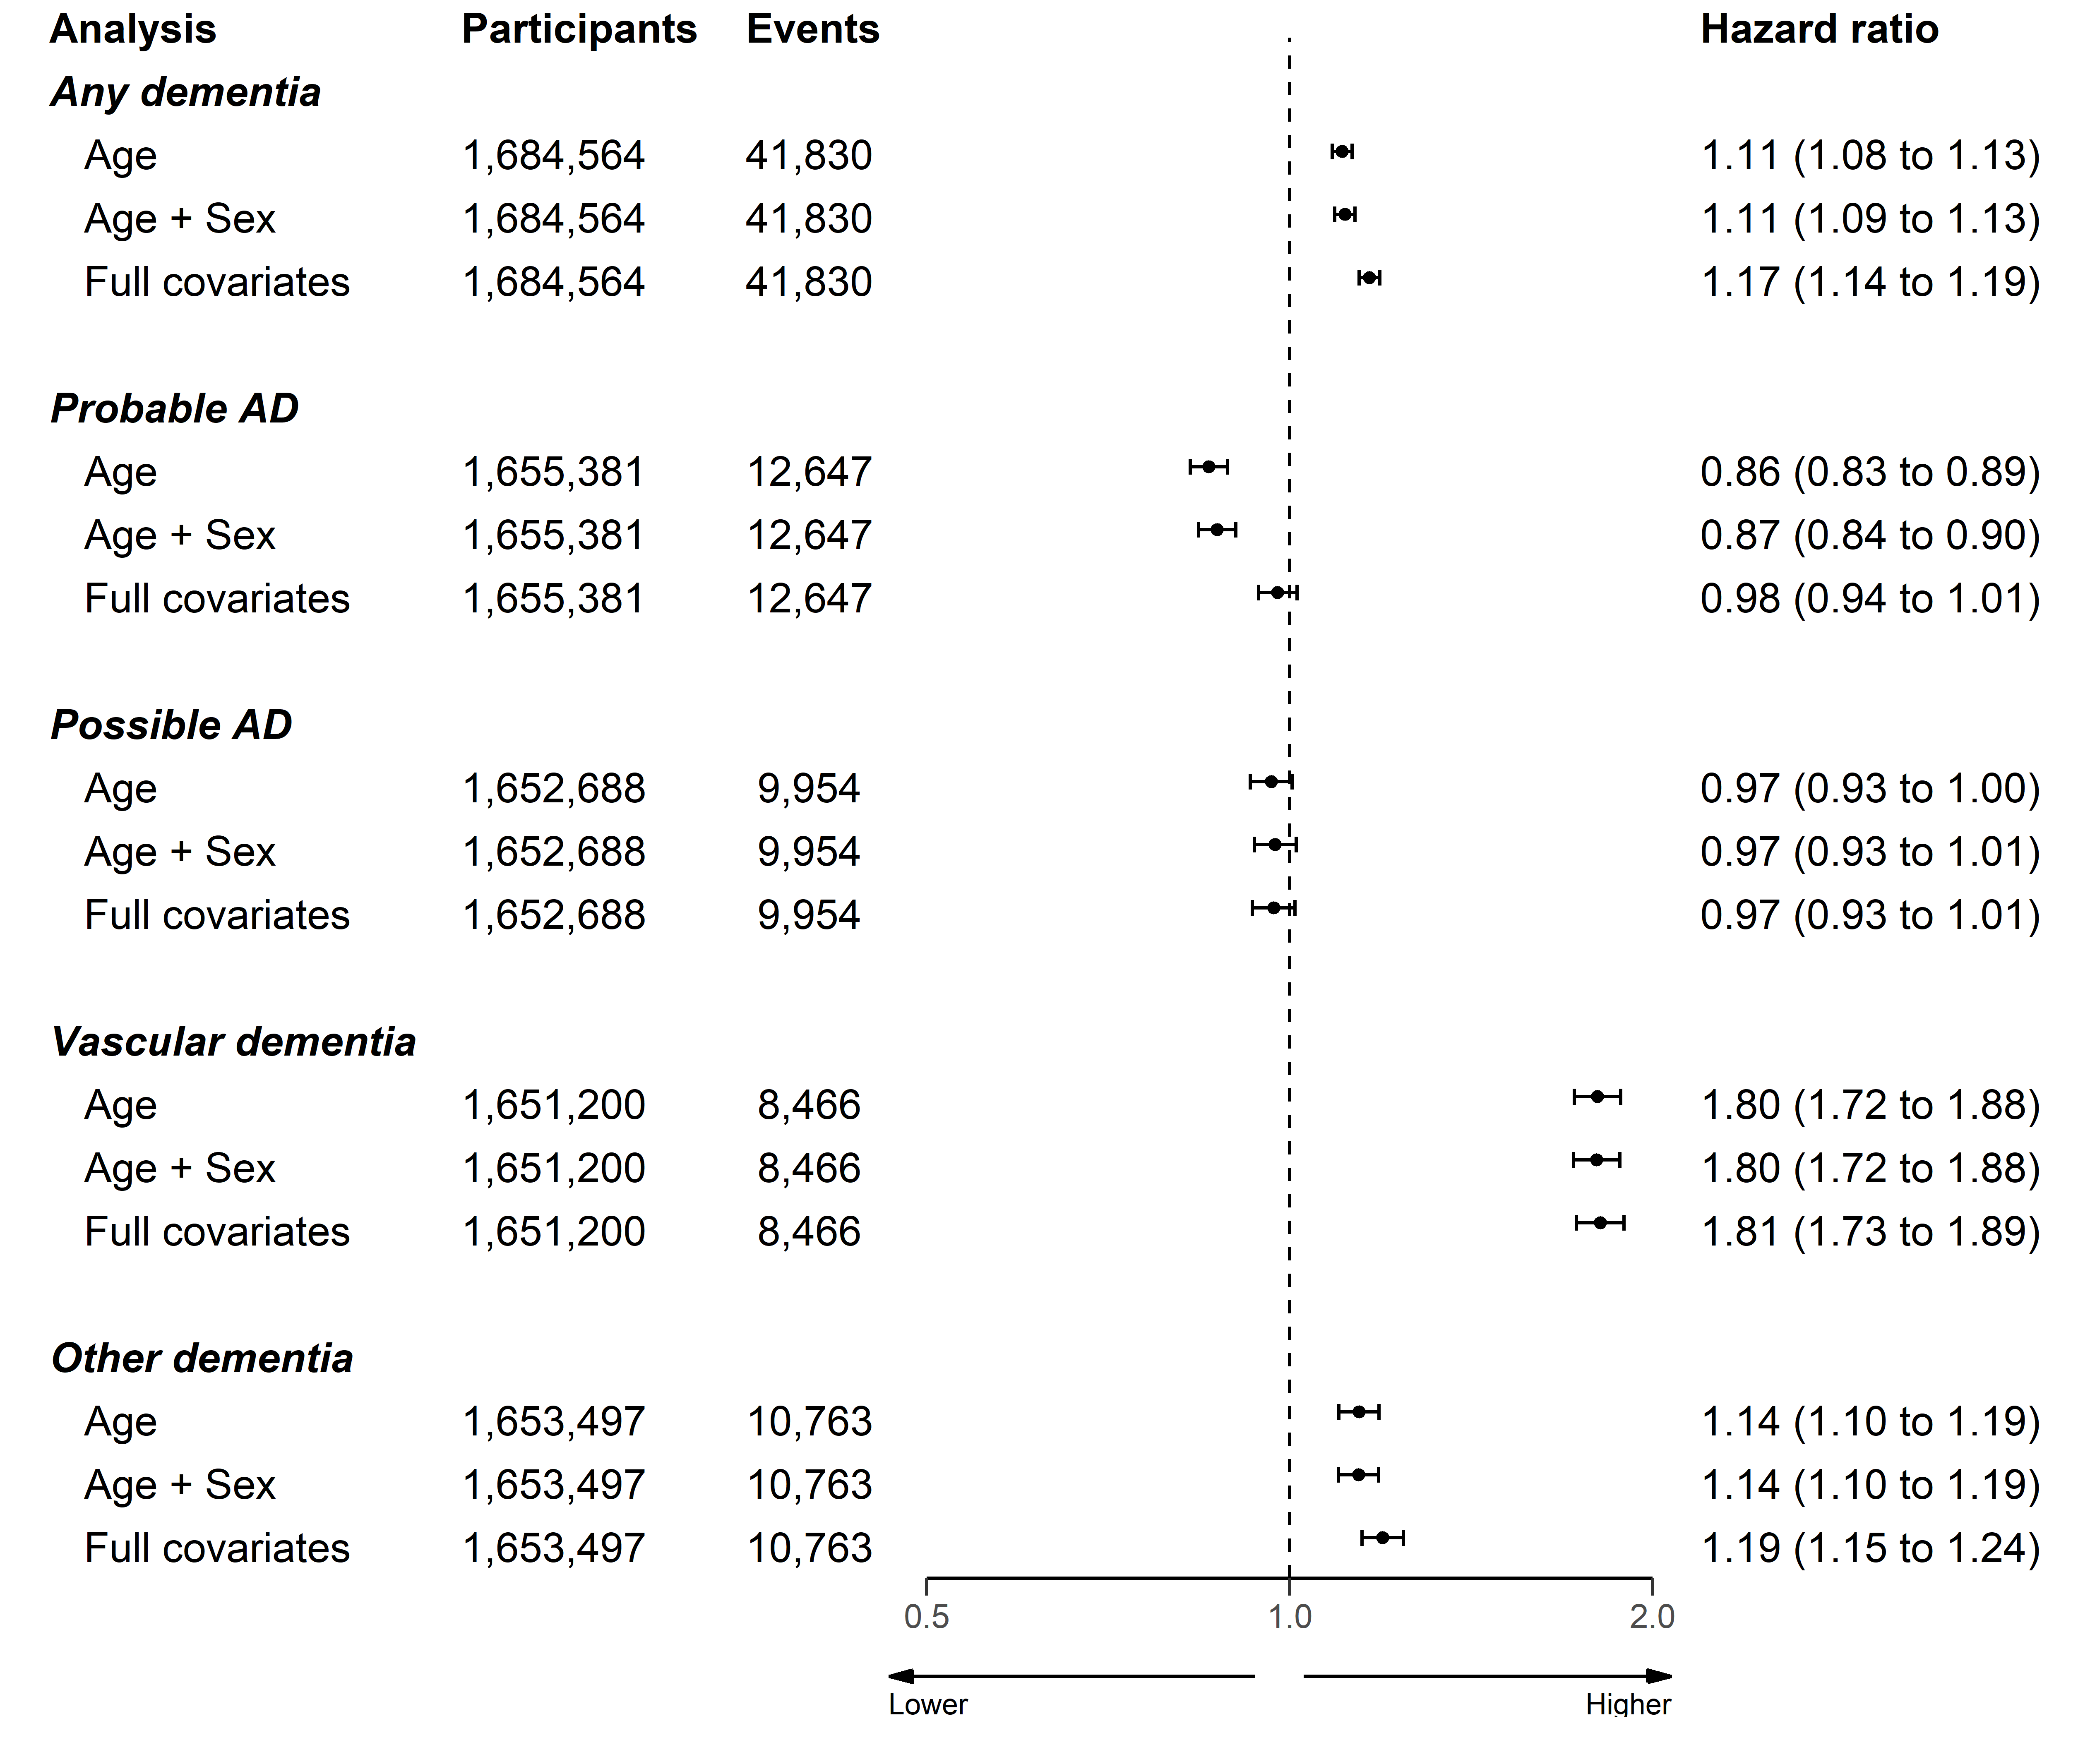
\includegraphics[width=1\linewidth]{figures/cprd-analysis/forester_unadjusted} \caption[Comparison of different combinations of covariates]{Results of three models adjusting for a different set of covariates.}\label{fig:unadjustedComparisonFig}
\end{figure}

~

\hypertarget{sensitivity-cohorts-entry-year}{%
\subsubsection{Sensitivity cohorts: Entry year}\label{sensitivity-cohorts-entry-year}}

When stratifying based on year of entry to the cohort, I observed no variation in risk by time period in any subgroup except for probable Alzheimer's disease (Figure \ref{fig:diagnosisTypeFig}).

~





\begin{figure}[H]
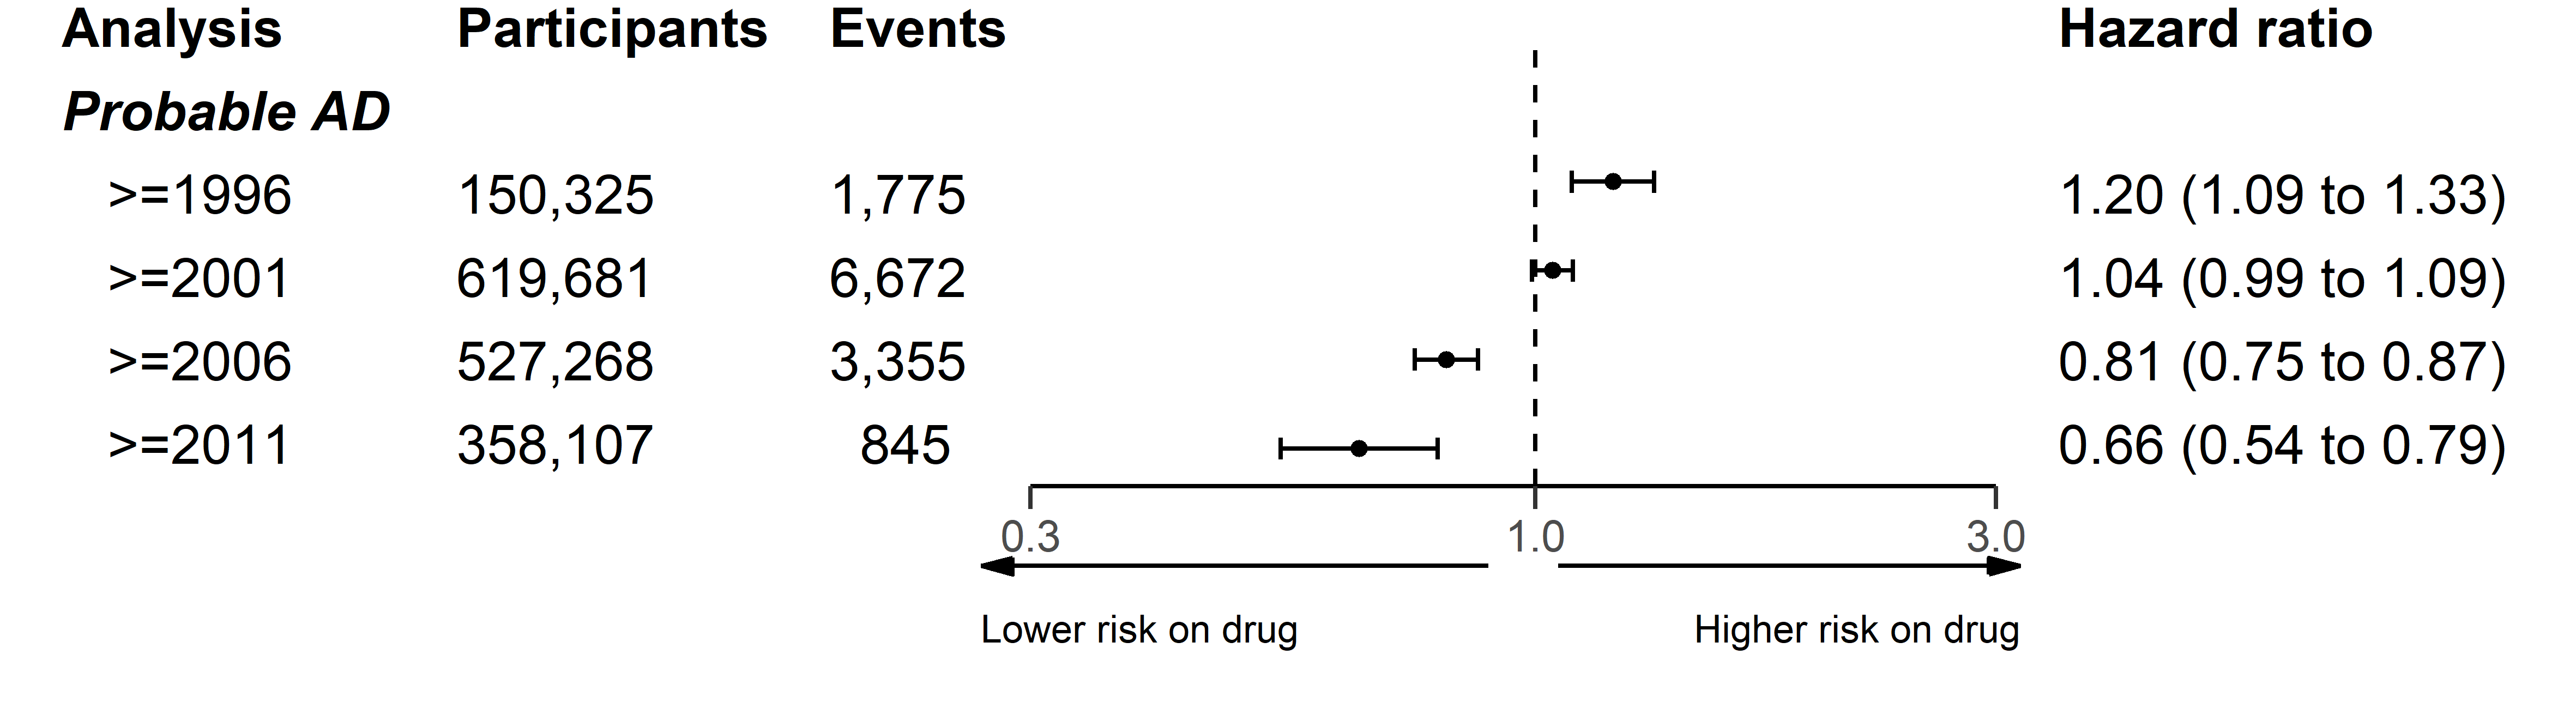
\includegraphics[width=1\linewidth]{figures/cprd-analysis/forester_cohort_entry} \caption[Sensitivity analysis: grouped year of entry]{Analysis of any lipid-regulating agent on probable AD outcome, stratified by grouped year of cohort entry.}\label{fig:diagnosisTypeFig}
\end{figure}

~

On the assumption that this variation could be caused by changes in the frequency of codes used to define probable AD in the cohort, I performed a \emph{post-hoc} investigation of the frequency of each diagnoses stratified by year of entry (Table \ref{tab:diagnosisType-table}). While the frequency of outcomes declines in more recent strata, likely due to the limited follow-up inherent to these groups, this decline in frequency is relatively constant across the dementia subtypes.

~





\begin{table}[H]

\caption[Frequency of diagnoses by grouped year of cohort entry]{\label{tab:diagnosisType-table}Frequency of diagnoses by grouped year of cohort entry}
\centering
\fontsize{7}{9}\selectfont
\begin{tabular}[t]{>{\raggedright\arraybackslash}p{5.33em}>{\centering\arraybackslash}p{5.33em}>{\centering\arraybackslash}p{5.33em}>{\centering\arraybackslash}p{5.33em}>{\centering\arraybackslash}p{5.33em}>{\centering\arraybackslash}p{5.33em}l}
\toprule
\textbf{\textbf{Year of cohort entry}} & \textbf{\textbf{No dementia}} & \textbf{\textbf{Probable AD}} & \textbf{\textbf{Possible AD}} & \textbf{\textbf{Vascular dementia}} & \textbf{\textbf{Other dementia}} & \textbf{\textbf{Total}}\\
\midrule
<=2000 & 148550 (95.9\%) & 1775 (1.1\%) & 1677 (1.1\%) & 1345 (0.9\%) & 1585 (1.0\%) & 154932\\
\midrule
2001-2005 & 613009 (96.3\%) & 6672 (1.0\%) & 5711 (0.9\%) & 4857 (0.8\%) & 6073 (1.0\%) & 636322\\
\midrule
2006-2010 & 523913 (98.1\%) & 3355 (0.6\%) & 2169 (0.4\%) & 1890 (0.4\%) & 2506 (0.5\%) & 533833\\
\midrule
2010< & 357262 (99.4\%) & 845 (0.2\%) & 397 (0.1\%) & 374 (0.1\%) & 599 (0.2\%) & 359477\\
\midrule
Total & 1642734 (97.5\%) & 12647 (0.8\%) & 9954 (0.6\%) & 8466 (0.5\%) & 10763 (0.6\%) & 1684564\\
\bottomrule
\end{tabular}
\end{table}

~

\hypertarget{sensitivity-cohorts-pregnancy}{%
\subsubsection{Sensitivity cohorts: Pregnancy}\label{sensitivity-cohorts-pregnancy}}

In the second sensitivity cohort, removing participants aged 55 and under at index from the analysis had minimal effect on the effect estimates (Figure \ref{fig:pregnancyFig}).

~





\begin{figure}[H]
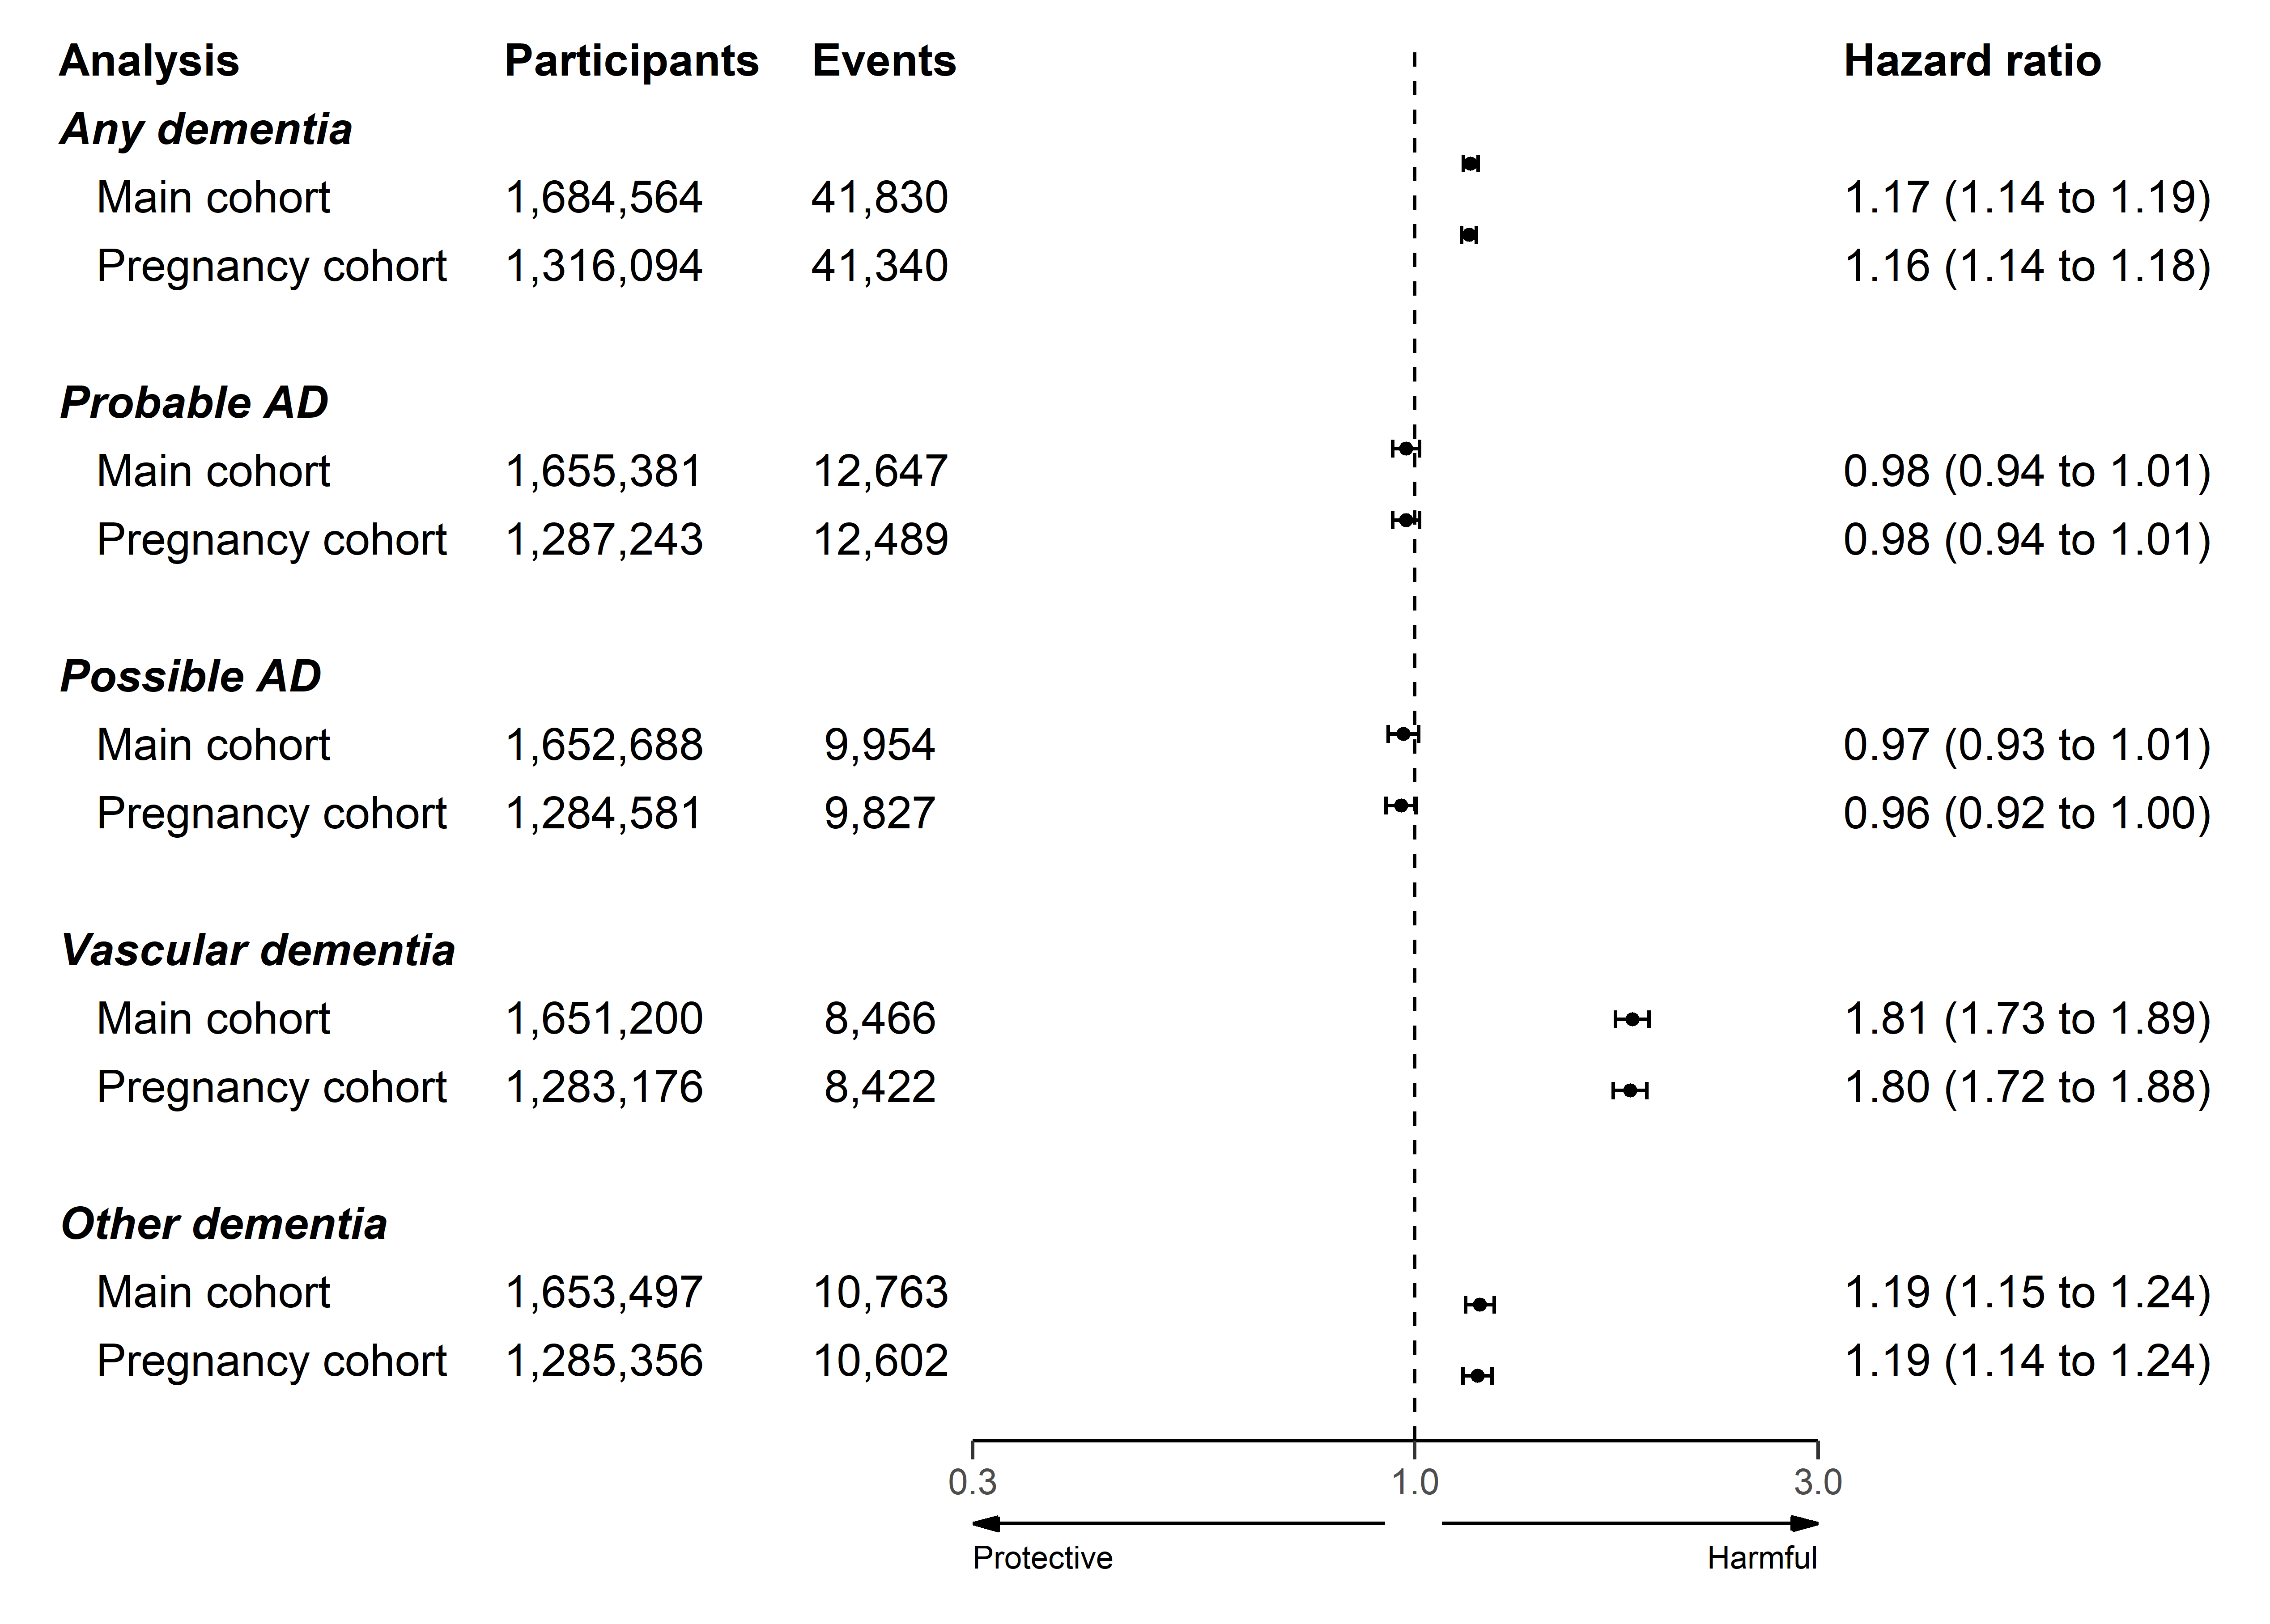
\includegraphics[width=1\linewidth]{figures/cprd-analysis/forester_pregnancy} \caption[Comparison of pregnancy analysis]{Comparison of analysis using main cohort and a cohort with potentially pregnany women removed.}\label{fig:pregnancyFig}
\end{figure}

~

\hypertarget{statin-properties-1}{%
\subsubsection{Statin properties}\label{statin-properties-1}}

In the cohort, statins with lipophilic properties were much more frequently prescribed than hydrophilic statins (Table \ref{tab:statinTypeTable-table}). Additionally, there is evidence for a increasing tendency to favour hydrophilic statins in recent years, as the proportion of lipophilic statins prescribed fell from 18.2\% in 1996-2000 to \textless1\% in 2011-2016.

~





\begin{table}[H]

\caption[Summary of statin properties (lipophilicity vs hydrophilicity).]{\label{tab:statinTypeTable-table}Summary of statin properties (lipophilicity vs hydrophilicity) by grouped year of prescription.}
\centering
\fontsize{7}{9}\selectfont
\begin{tabular}[t]{lccc}
\toprule
\textbf{\textbf{Prescription Year Group}} & \textbf{\textbf{Hydrophilic}} & \textbf{\textbf{Lipophilic}} & \textbf{\textbf{Total}}\\
\midrule
<=2000 & 7037 (18.2\%) & 31531 (81.8\%) & 38568\\
\midrule
2001-2005 & 21427 (10.3\%) & 187018 (89.7\%) & 208445\\
\midrule
2006-2010 & 3566 (1.6\%) & 217726 (98.4\%) & 221292\\
\midrule
2010< & 1115 (0.9\%) & 119035 (99.1\%) & 120150\\
\bottomrule
\end{tabular}
\end{table}

~

When stratifying by statin properties, hydrophilic statins were less harmful in the any, vascular and other dementias outcomes compared to lipophilic statins (Figure \ref{fig:statinTypeFig}). Additionally, in the AD outcomes, hydrophilic statins were associated with a small reduction in risk, compared to the weak evidence for an effect for lipophilic statins.

~





\begin{figure}[H]
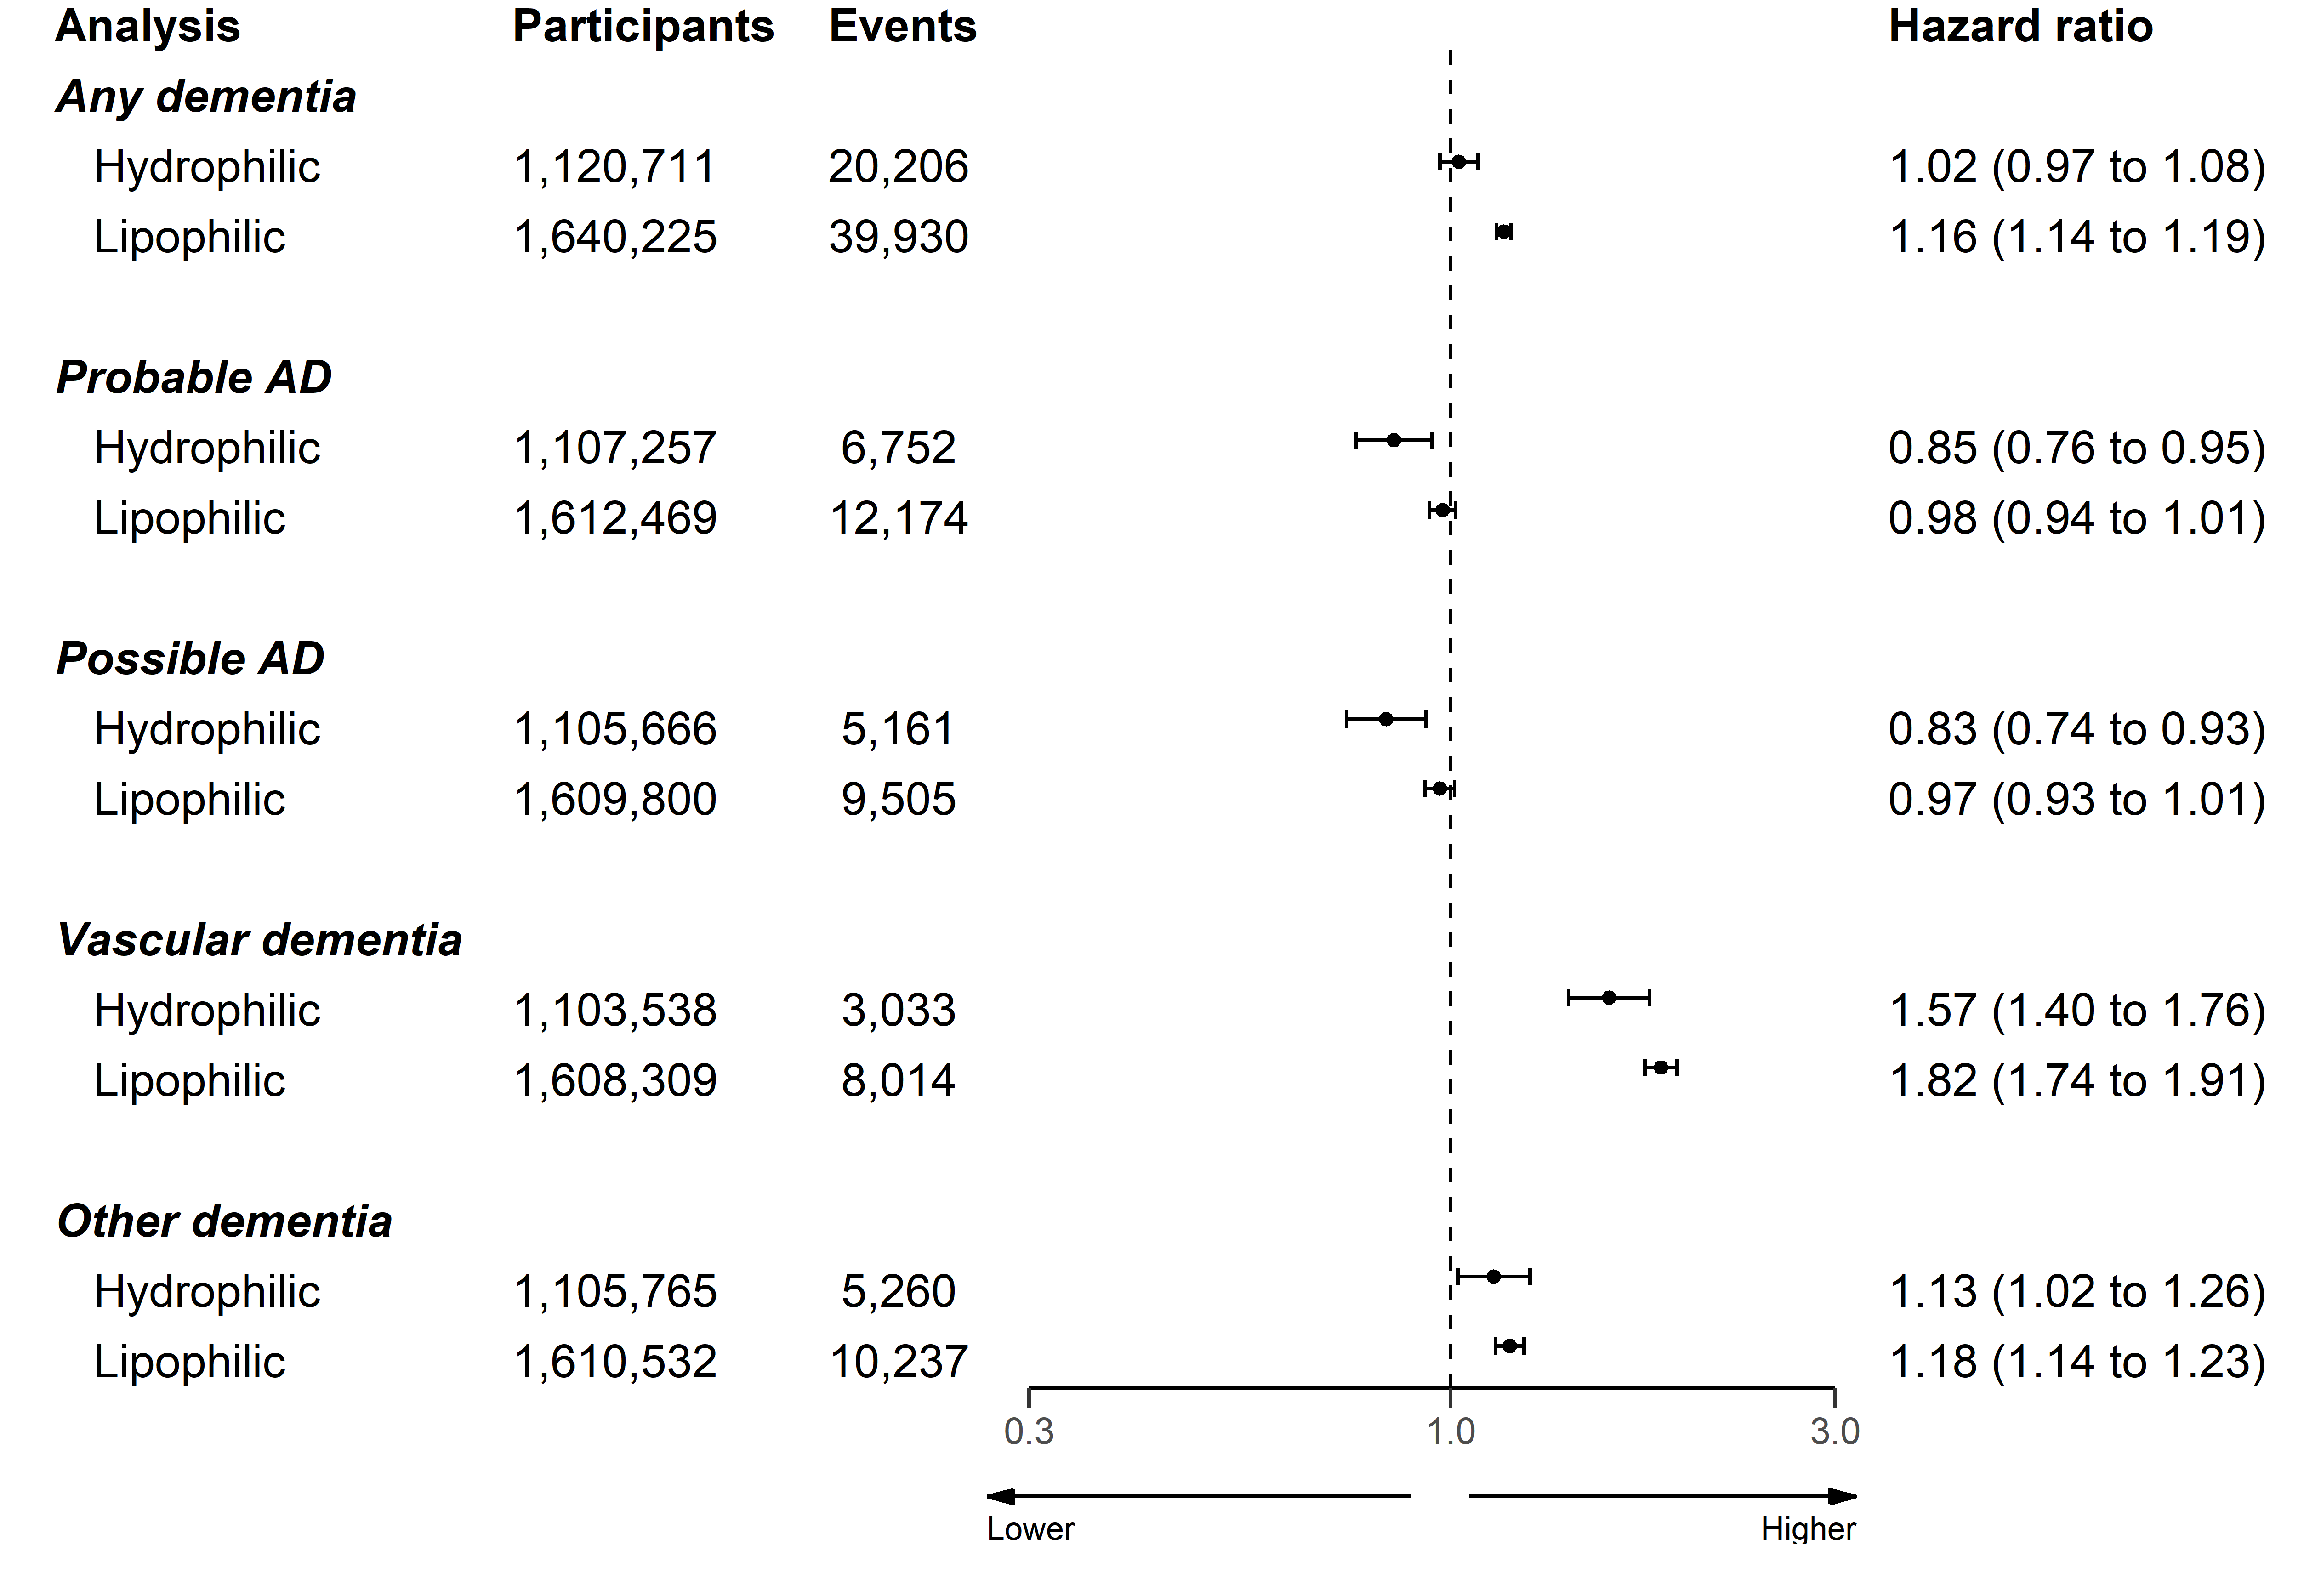
\includegraphics[width=1\linewidth]{figures/cprd-analysis/forester_sta_type} \caption[Analysis stratified by statin properties]{Analysis stratified by statin properties (hydrophilic vs lipophilic)}\label{fig:statinTypeFig}
\end{figure}

~

\hypertarget{comparing-codelists}{%
\subsubsection{Impact of dementia code lists}\label{comparing-codelists}}

When using the Smeeth \emph{et al.} code lists to define dementia outcomes, effect estimates of HR: 1.19 (95\%CI: 1.07-1.32) and HR: 1.33 (95\%CI: 1.26-1.42) were obtained for the Alzheimer's disease and non-Alzheimer's (``other'') dementia outcomes, respectively.

~

\hypertarget{discussion-2}{%
\section{Discussion}\label{discussion-2}}

\hypertarget{summary-of-findings-1}{%
\subsection{Summary of findings}\label{summary-of-findings-1}}

Lipid-regulating agents showed little evidence of an association with probable and possible Alzheimer's disease when compared to no treatment, but were associated with increased risk of an all-cause dementia, vascular dementia and other dementias diagnosis. The estimate observed in each case was driven by the statin subgroup, which included a substantial majority of participants. For the other drug classes, no association was found with any outcome, with two exceptions being that ezetimibe was associated with increased risk of vascular and other dementias, while fibrates were associated with increase risk of all-cause dementia and probable Alzheimer's disease.

The effect estimates were robust to the exclusion of potentially pregnant participants, and for all outcomes except probable AD, no variation across grouped year of entry was observed. When looking at the statin subgroup alone, statin properties appeared to have a modifying effect, with hydrophilic statins being less harmful in the any, vascular and other dementias outcomes compared to lipophilic statins.

~

\hypertarget{interpretation-of-results}{%
\subsection{Interpretation of results}\label{interpretation-of-results}}

This section will expand on a potential explanation for the observed results detailed above. However, as the comparison of evidence across different sources is the aim of the triangulation exercise presented in later chapters, the section will not provide a detailed comparison with other published literature, except where needed to illustrate a methodological point. For a detailed comparison of the result presented above with the existing evidence base identified by the systematic review (Chapter \ref{sys-rev-heading}), see Chapter \ref{tri-heading}.

\textbf{{[}Feedback requested: How much should I be cross-referencing with the systematic review at this stage? Or should I keep it self-contained, and then provide a comparison across the review/CPRD/IPD analyses as the first part of the triangulation chapter?{]}}

~

\hypertarget{confounding-by-indication}{%
\subsubsection{Confounding by indication}\label{confounding-by-indication}}

A likely explanation for the observed increased risk of dementia outcomes with a vascular component (e.g.~vascular and other dementias) with lipid-regulating agent use, and an important limitation of this analysis, is residual ``confounding by indication''. While the term has been used to describe different source of bias in epidemiological analyses,\textsuperscript{\protect\hyperlink{ref-salas1999}{294}} it is used here to described the role of risk factors that both prompt treatment and increase the risk of the outcome, thus causing a distorted positive association between the treatment and outcome (see Figure \ref{fig:indicationBias}). In causal inference nomenclature, statins and dementia are said to be \emph{d}-connected as there is an open ``backdoor'' path between them via the uncontrolled confounders.\textsuperscript{\protect\hyperlink{ref-suttorp2015}{295}} In the context of this analysis, the confounding variable (or, more likely, variables) would prompt prescription of statins but also represent a vascular risk factor that contributes to the development of the vascular dementia.

~\\




\begin{figure}[H]

{\centering 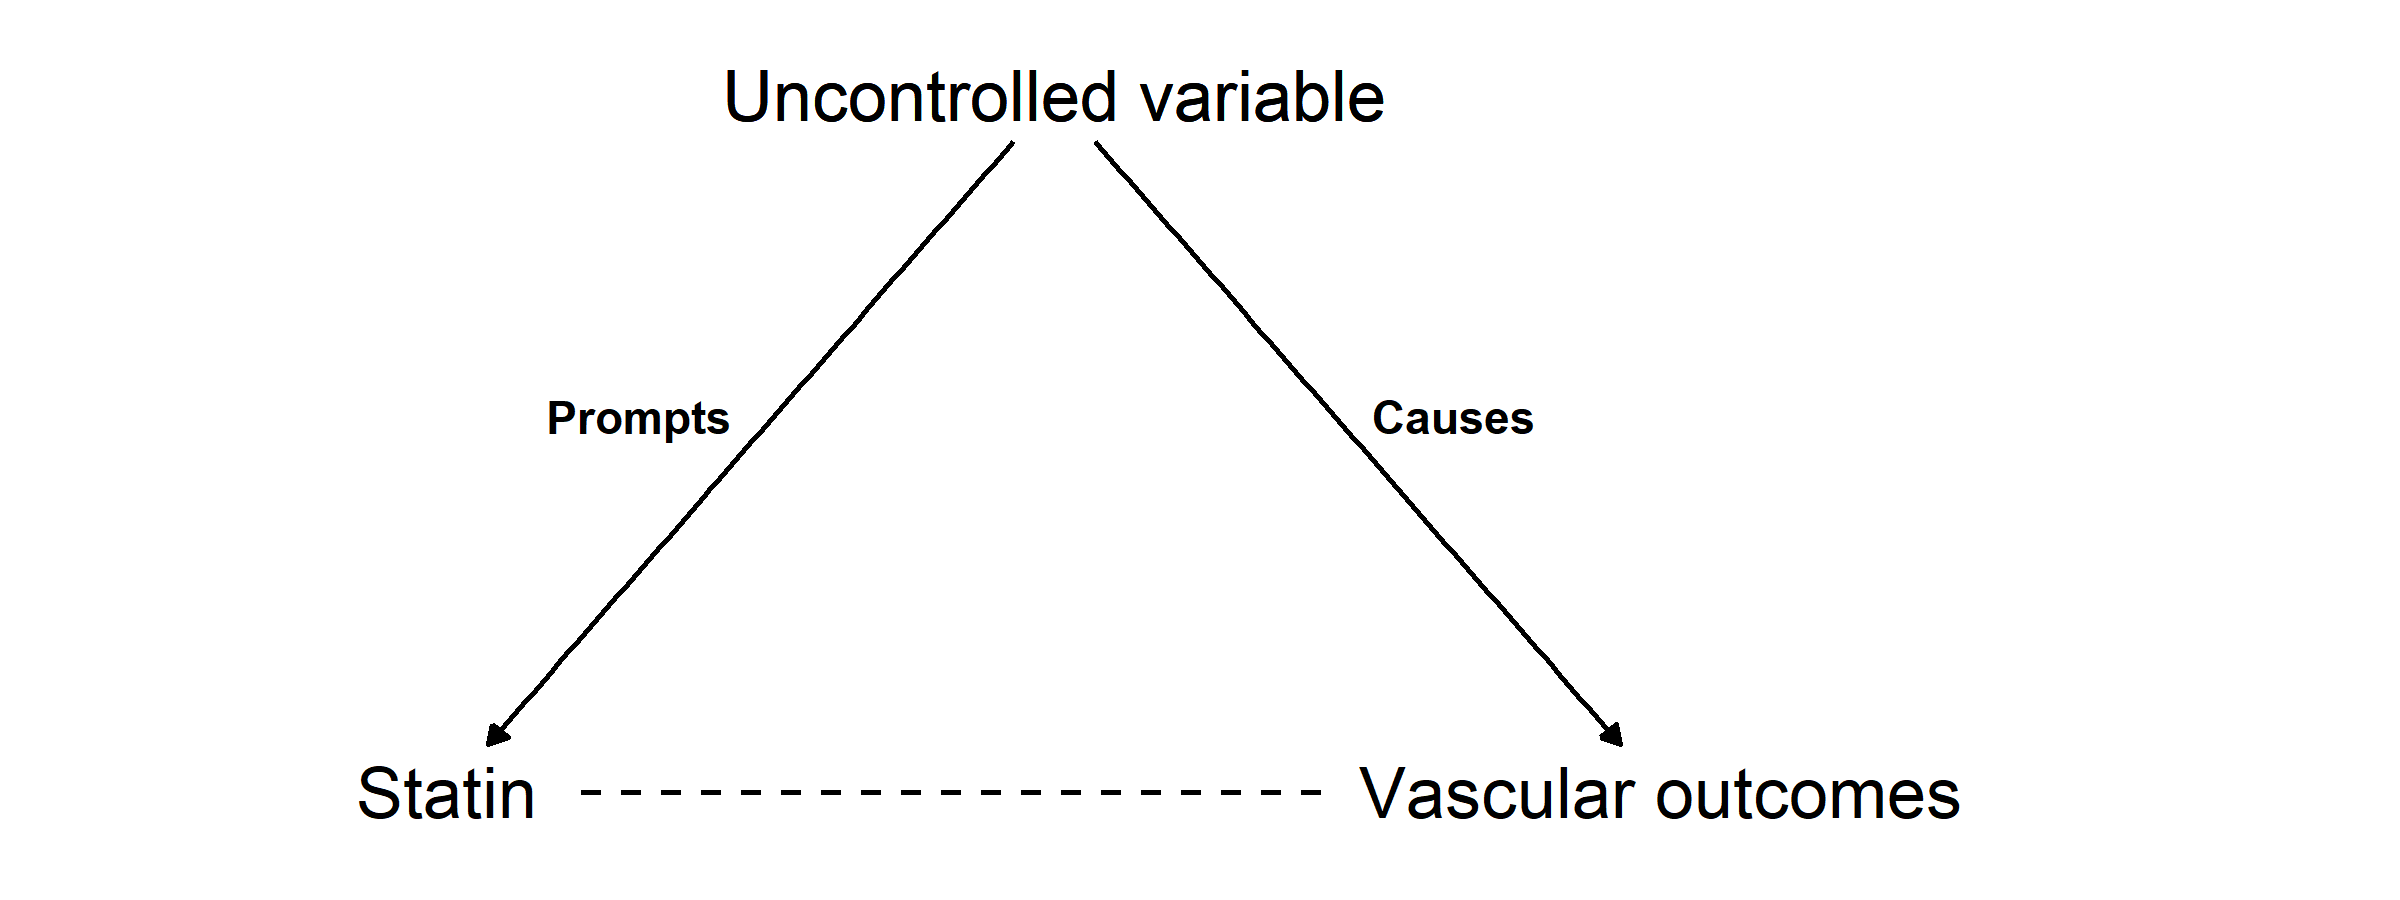
\includegraphics[width=0.8\linewidth]{figures/cprd-analysis/indicationBias} 

}

\caption[Confounding by indication causal diagram]{Causal diagram (directed acyclic graph) illustrating how confounding by indication could induce a positive association between statins and vascular dementia.}\label{fig:indicationBias}
\end{figure}

~

Conditioning entry into the study on being either ``at-risk'' or already diagnosed with hypercholesterolemia was employed in a pre-emptive attempt to mitigate confounding by indication, but evidence from the control outcomes suggests this was unsuccessful. The slight harmful effect for the backpain outcome is substantially smaller that that observed for the ischemic heart disease outcome, indicating that the majority of the uncontrolled confounding is likely related to vascular factors.

In line with this, an increasingly harmful effect is observed when moving from the probable and possible Alzheimer's disease outcome to the other dementias outcome, and finally to the vascular dementia outcomes. This pattern suggests that the strength of the residual confounding by indication increases as the proportion of cases with a vascular component in an outcome definition increases. Given confounding related to vascular factors, this pattern is also expected given the decision tree for assigning outcomes in the presence of greater than one dementia code. Under this system, the Alzheimer's disease outcomes require a ``pure'' condition and the presence of any vascular or other dementias codes excludes participants from this group (Figure \ref{fig:decisionTreeFig}).

A review of other available literature suggests that this observation (a harmful effect of lipid-regulating agents on vascular-related outcomes) is not unusual. Using a conventional epidemiological technique, a previous analysis also found an increased risk of coronary heart disease (analogous to the ischemic heart disease outcome used in this analysis) in those taking statins (HR: 1.31, 95\%CI: 1.04-1.66).\textsuperscript{\protect\hyperlink{ref-danaei2013b}{296}} Controlling for confounding by indication in that study through the use of a trial emulation analysis gave an estimate of 0.89 (95\%CI: 0.73-1.09), a comparable though less precise estimate to that observed in RCTs of statin use (0.73, 95\%CI: 0.67-0.80).\textsuperscript{\protect\hyperlink{ref-taylor2013}{297}}

Given the absence of vascular dementia in the published literature, as highlighted in the previous chapter (see Section \ref{sys-rev-pub-bias}), the unexpected increase in vascular dementia risk with statin use is particularly interesting It is possible that previous research encountered similar methodological issues to this analysis, and via a publication bias mechanism where unexpected or assumedly incorrect results are less likely to be published, the results from these analyses did not make it into the evidence base.

~

~

\hypertarget{statin-properties-2}{%
\subsubsection{Statin properties}\label{statin-properties-2}}

This analysis found that hydrophilic statins were less harmful in the any, vascular and other dementias outcomes compared to lipophilic statins, and were associated with a small reduction in the risk of the probable and possible AD outcomes. The relative precision of the estimates in each group is expected, as the two most commonly prescribed statins are lipophilic (simvastatin and atorvastatin).\textsuperscript{\protect\hyperlink{ref-newman2019}{298}}

A widely discussed concept in the literature surrounding statin use and cognitive outcomes is the fact that lipophilic statins are more likely to be able to cross the blood brain barrier, and so have a more potent protective effect by directly lowering brain cholesterol.\textsuperscript{\protect\hyperlink{ref-shepardson2011}{299}} My findings that hydrophilic statins appear to be more protective/less harmful than their lipophilic counterparts runs counter to this assertion.

An initial interpretation of the the different association observed in the two groups was that the lipophilic statins may be more potent, and so are prescribed to patients with a higher underlying vascular load, leading to increased confounding by indication in this group. However, the statin with the strongest lipid lowering effect that is available via the NHS, rosuvastatin, is hydrophobic.

\textbf{{[}Yoav, are there are particular indications/contraindications for statins with different properties? And any general comments on the interpretation of these findings would be welcome!{]}}

~

\hypertarget{impact-of-code-lists}{%
\subsubsection{Impact of code lists}\label{impact-of-code-lists}}

As part of a sensitivity analysis exploring the impact of outcome code-lists, I used definitions for Alzheimer's disease and other dementias obtained from a previously published paper (Smeeth \emph{et al.}).\textsuperscript{\protect\hyperlink{ref-smeeth2009}{292}} Using these lists in my analytical set-up, I found a harmful association of statin use with both outcomes.

TThis finding disagrees with the results of the original analysis, which found evidence for a protective effect of statin use on all-cause dementia (HR: 0.81, 95\%CI: 0.69-0.96) and non-AD dementia (HR: 0.82, 95\%CI: 0.69-0.97), but little evidence of an effect on AD (HR: 0.81, 95\%CI: 0.49-1.35).

However, comparison of the results obtained using the two sets of code lists was deemed less useful following a detailed comparison of the codes used. While all of the codes used to define Alzheimer's in the Smeeth \emph{et al.} paper are included in the probable Alzheimer's code-list (see Figure \ref{fig:smeethComparison}), I included several additional codes used to define this outcome (including, for example, ``Eu00013: {[}X{]}AD disease type 2''). Additionally, several of the codes used to define ``Possible Alzheimer's'' in this analysis are included in the ``Other dementia'' code list used by Smeeth.

~





\begin{figure}[H]
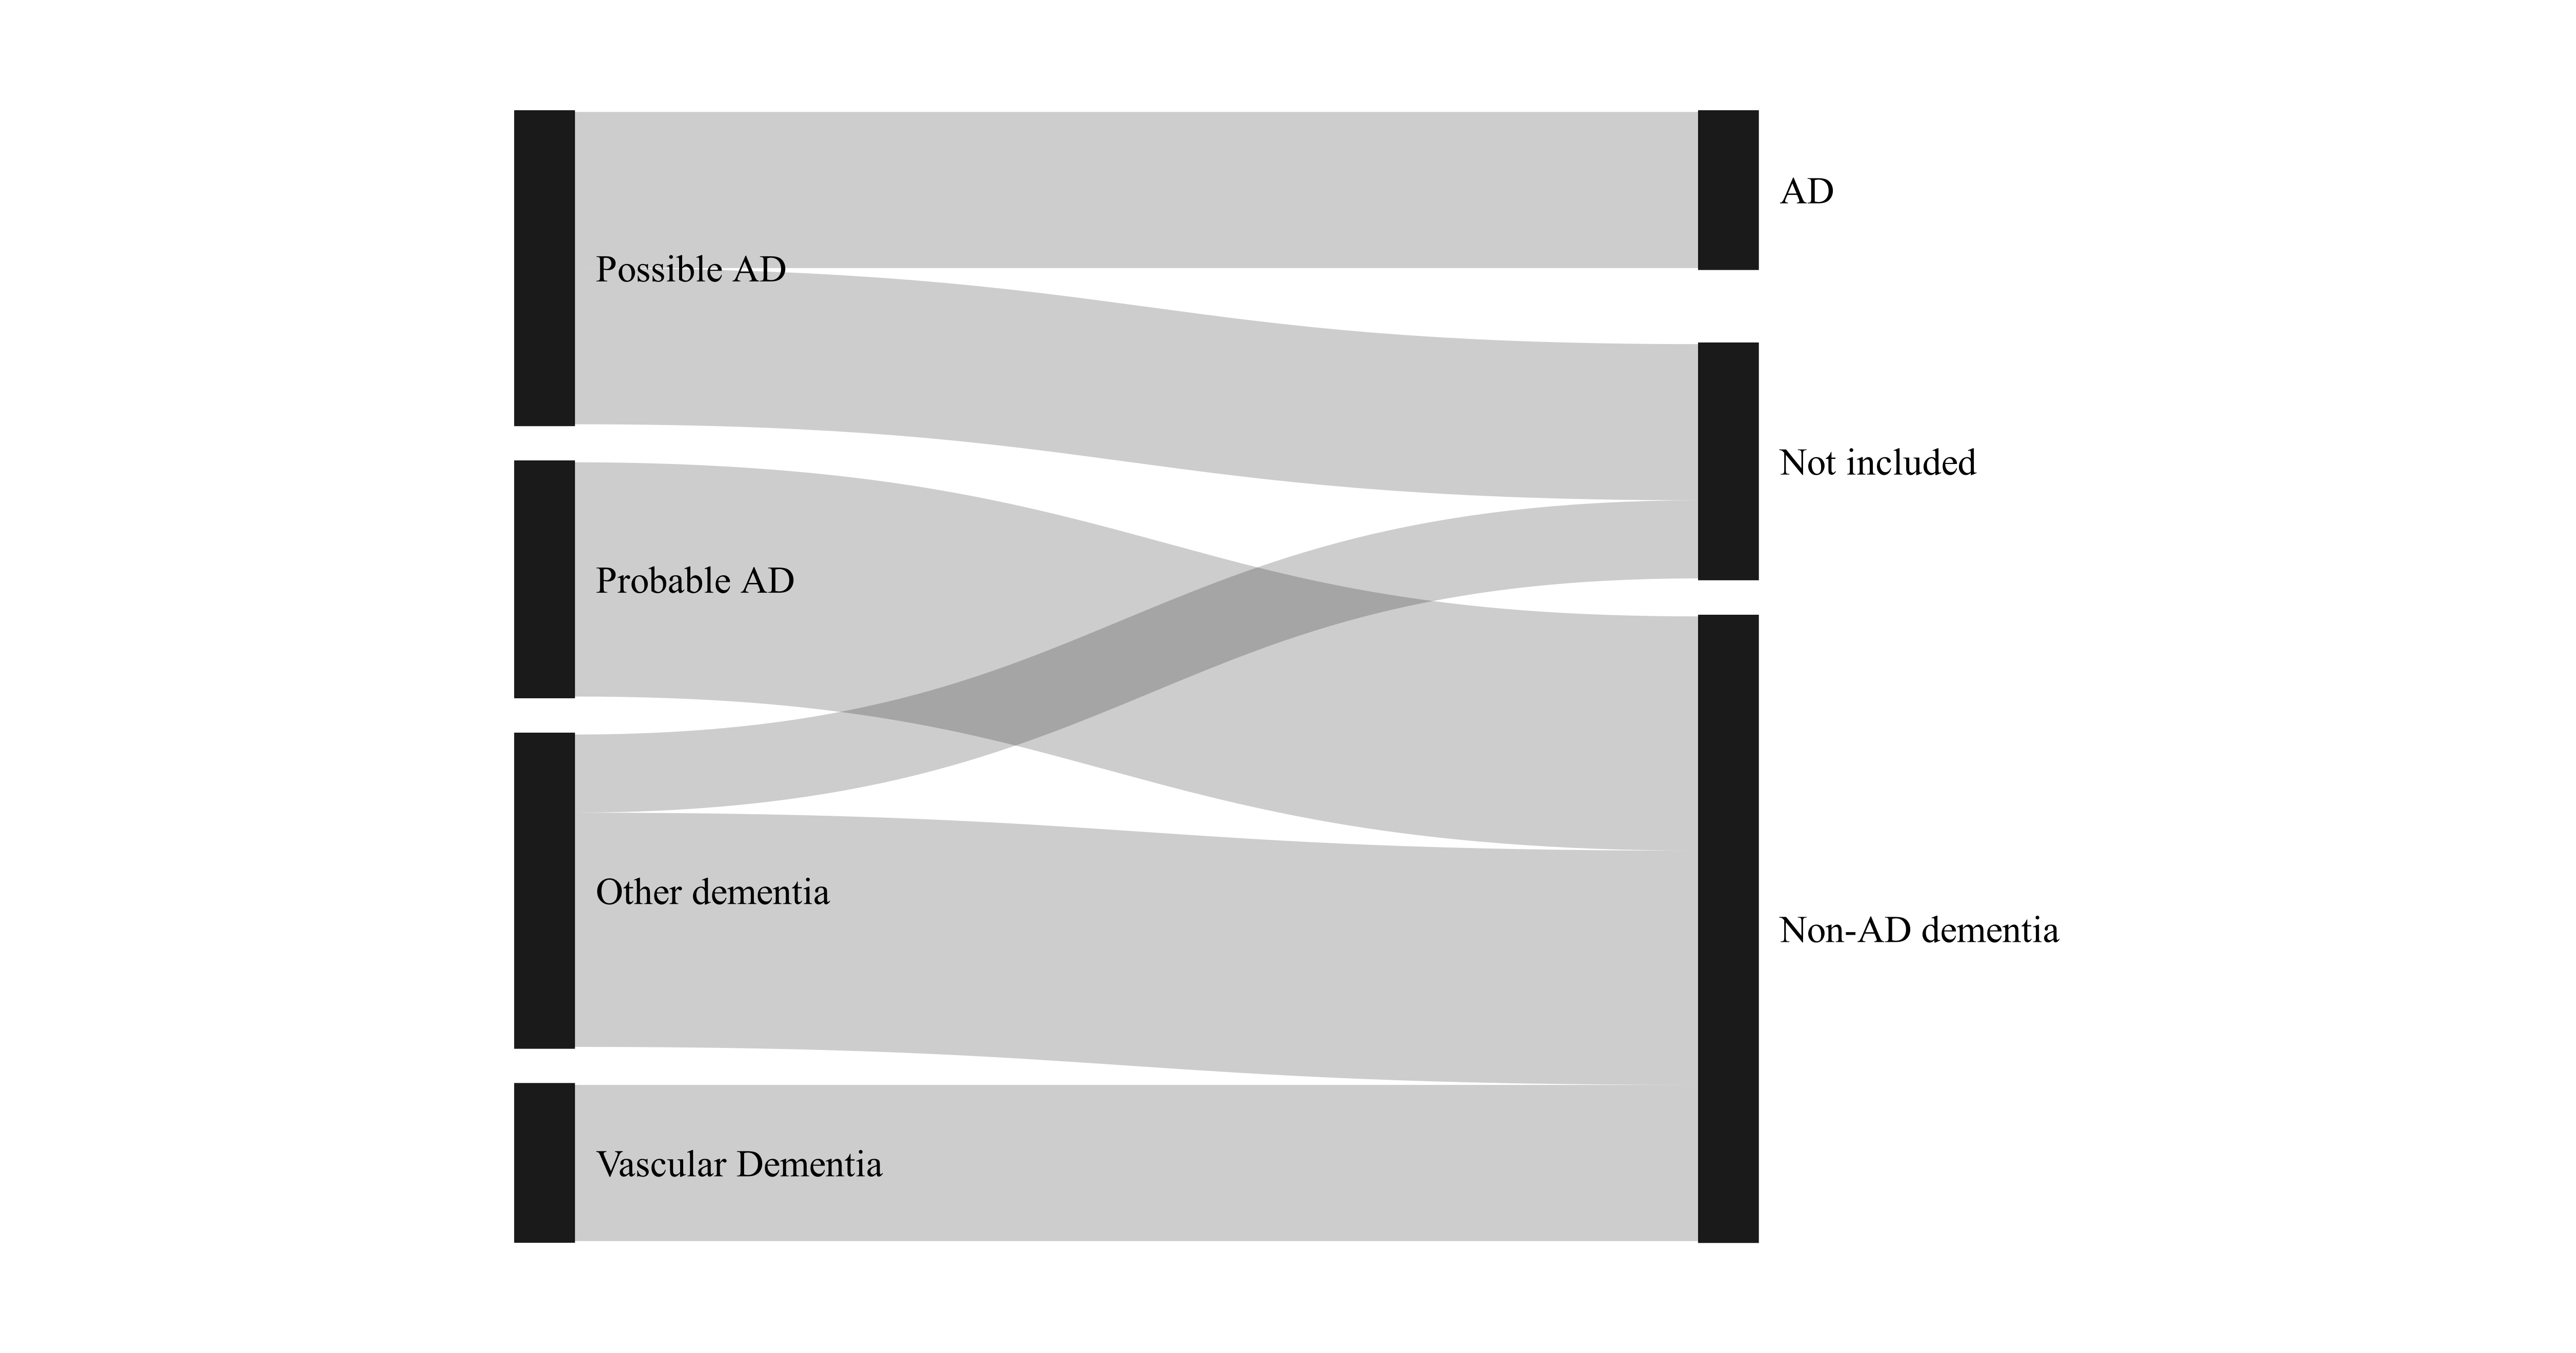
\includegraphics[width=1\linewidth]{figures/cprd-analysis/sankey_diagram} \caption[Comparison of code used in this analysis with those used in the Smeeth et al.~2010 paper]{Sankey diagram comparing the codes used in this analysis with those used in the Smeeth \emph{et al} paper.\textsuperscript{\protect\hyperlink{ref-smeeth2009}{292}} The outcomes and number of codes contributing to each are presented (the Smeeth \emph{et al} outcomes are on the right hand side of the figure). The joining lines showing the overlap between the categories in the two analyses.}\label{fig:smeethComparison}
\end{figure}

This analysis serves to illustrative the importance of the code lists chosen to define the outcomes of interest, particularly if they are used to define competing outcomes (e.g.~AD vs non-AD dementia). This different codes used by Smeeth \emph{et al.}, in addition to an analytical approach that adjusted for covariates defined after the index date, may go some way to explaining why our analysis obtained different results despite the substantial overlap in the data sources used.

~

\hypertarget{strengths-and-limitations-1}{%
\subsection{Strengths and limitations}\label{strengths-and-limitations-1}}

The primary strength of this analysis is the relative size of the CPRD and length of follow-up. Having reviewed the existing literature, as identified by the systematic review in Chapter \ref{sys-rev-heading}, this analysis of 1,684,564 participants is one of the largest available studies of this research question. Additionally, this analysis followed LRA users and non-users from a common index date, using a time-updating treatment indicator to correctly assign time-at-risk to the exposed and unexposed groups. This approach has been less commonly used in the literature and allows for the mitigation of potential immortal time bias. Finally, it is one of the few that provide evidence on the association of lipid-regulating agent use and vascular and other dementias.

However, the findings of this analysis are subject to several limitations in addition to the confounding by indication discussed above. There is a strong possibility of differential misclassification of dementia-related conditions based on the exposure.\textsuperscript{\protect\hyperlink{ref-porta2014dictionary}{300}} As an illustrative example, those with memory complaints may be more likely to be classified as vascular dementia than Alzheimer's disease if their medical records contains prescriptions for lipid-regulating agents. Further, there is a potential for general non-differential misclassification of the outcome due to the varying positive predictive value of electronic health record code lists to identify dementia cases.\textsuperscript{\protect\hyperlink{ref-mcguinness2019validity}{258},\protect\hyperlink{ref-wilkinson2018}{259}}

Misclassification of outcomes is not the only issue introduced by the use of EHR codes to define outcomes. Comparing and contrasting between different studies is particularly difficult because of the impact that the use of different code list can have on the analysis, as illustrated by the discrepancy between the results when using the codes lists defined for this study and those used by Smeeth \emph{et al}. This presents a particular challenge in comparing research across different time-periods and coding systems, particularly the unexpected results I obtained for the vascular and other dementias outcomes.

A further limitation stems from the possibility of uncontrolled confounding due to genetic factors. Number of ApoE \(\epsilon4\) alleles represents the strongest genetic risk factor for Alzheimer's disease, but also substantially increases LDL-c levels,\textsuperscript{\protect\hyperlink{ref-bennet2007}{301}} potentially prompting treatment with a statin or other lipid regulating agent. I was unable to control for ApoE genotype in this analysis as I did not have access to genetic data on participants. As a result, any protective association between LRA use and the Alzheimer's disease outcomes may be masked by residual negative confounding by ApoE.

Finally, as with many studies of dementia, there is a risk of reverse causation in my analysis. Dementia and associated conditions have a long prodromal period, during which preclinical disease could cause indications for the prescription of a lipid-regulating agent.

~

\hypertarget{cprd-data-avail}{%
\subsection{Enabling easy synthesis of this analysis}\label{cprd-data-avail}}

The raw data supporting this analysis is not publicly available, as access to the CPRD data is controlled by a data monitoring committee. However, when data are not readily available, sharing the analysis code and summary statistics represents a way for readers to validate the findings.\textsuperscript{\protect\hyperlink{ref-goldacre2019c}{302}}

In light of this and my own experiences in attempting to extract information for papers assessing preventative treatments, as documented in Section \ref{sys-rev-open-data}, the outputs from this analysis have been made readily available. All code, Read code lists and summary statistics (namely the tables presented in this chapter plus summary tables of effect estimates) can be downloaded in a machine readable format from the archived repository for this project (Zotero DOI: \textbf{TBC}). This open approach should enable easy inclusion of this analysis in future evidence synthesis exercises, allowing new work to build on that presented here.

~

\hypertarget{conclusions-1}{%
\subsection{Conclusions}\label{conclusions-1}}

This chapter has provided new evidence on the association of lipid-regulating agents with incidence of all-cause dementia, Alzheimer's disease, vascular dementia, and other dementia. It made use of a large scale electronic health record database, the CPRD, and employed a time-varying Cox proportional hazards model to account for potential immortal time bias.

It found little evidence for an effect of lipid-regulating agents on probable or possible Alzheimer's disease. However, lipid-regulating agent use was associated with an increased risk of all-cause, vascular and other dementias. In all cases, the estimated associations were driven by those observed in the statin subgroup, which comprised the majority of exposed participants in this cohort.

This chapter attempted to account for important sources of bias and provide a comparison with other available literature, as identified in the systematic review presented in Chapter \ref{sys-rev-heading}. However, there is a strong potential for uncontrolled confounding by indication and differential misclassification of the outcome on the basis of exposure, which raises questions about the findings, in particular the unexpected increase in risk of vascular dementia associated with statin use. The presence of bias is supported by our findings for the negative and positive control outcomes used, which provide some evidence of uncontrolled vascular confounders that may both prompt LRA prescription and increase risk of dementia outcomes with a vscular component. Future research using large scale electronic health records should aim to address these limitations, potentially by using a analytical design that more closely emulates a trial.\textsuperscript{\protect\hyperlink{ref-danaei2013b}{296}}

Regardless, this analysis has provided an additional source of evidence for the triangulation exercise presented in Chapter \ref{discussion-heading}. In the following Chapter, the dataset described here is incorporated along with several other datasets as part of an individual patient data analysis to investigate the association of blood lipid levels with incidence of dementia outcomes directly, rather than via the proxy of lipid-regulating treatment.

\newpage

\hypertarget{references-3}{%
\section{References}\label{references-3}}



\hypertarget{ipd-heading}{%
\chapter{Individual participant data meta-analysis}\label{ipd-heading}}

\minitoc 

\hypertarget{lay-summary-4}{%
\section{Lay Summary}\label{lay-summary-4}}

As part of a broader investigation into the relationship between lipid levels and dementia risk, I applied for access to 37 unique data sources containing information on these variables. However, only a small proportion of these data sources (n = 3, 8.1\%) provided me with access.

The resulting analysis did not suggest an effect of any lipid fraction (total cholesterol, LDL-c, HDL-c, or triglycerides) on any dementia outcome. In addition, patients characteristics such as age and sex did not have any impact on the relationship of lipid fractions and dementia outcomes.

Finally, the reasons for the low response rate are explored and future studies to investigate how data access rates could be improved are suggested.

~

\hypertarget{introduction-2}{%
\section{Introduction}\label{introduction-2}}

Individual patient data meta-analyses are considered to be the gold standard form of evidence synthesis, allowing for the application of a common selection model and analytical approach across all identified cohorts. They are particularly useful for investigating the impact of patient-level characteristics, something that is not possible with aggregate data unless the results have been explicitly stratified by the characteristic of interest.

While the systematic review presented in Chapter \ref{sys-rev-heading} did not provide strong evidence for an effect of age at lipid measurement or patient sex on the relationship between lipids and dementia, the number of included studies in the lipid fraction meta-analyses were very small, due to both the relatively small number of studies reporting on this exposure and the poor reporting of smmary statistics of patient characteristics.

As such, the aims of this analysis were two fold: firstly, to perform a individual patient data meta-analysis across identified cohorts to examine the impact of patient age-at-measurement and sex on the effect of lipids on dementia; and secondly, to expand the evidence base for the effect of lipids on dementia outcomes by incorporating previously unanalysed cohorts contained in the Dementia Platform UK, a large consortia of dementia cohorts.

~

\hypertarget{methods-2}{%
\section{Methods}\label{methods-2}}

\hypertarget{eligibility-criteria}{%
\subsection{Eligibility criteria}\label{eligibility-criteria}}

Eligible data sources were defined as those that contained lipid measurements and lipids reported/available as a continuous measure, Data sources which were cross-sectional, either by design or due to the available data (e.g.~a study conducted multiple waves, but onyl data from a single wave could be accessed) were excluded. Similarly, due to the limited time-frame, studies making use of population-level electronic health records, which often require an extensive project proposals in order to gain access to the data, were ineligible due to the time and cost involved in applying. The one exception to this was data from the CPRD, which I already had access to as part of the analysis reported in Chapter \ref(cprd-analysis-heading).

\hypertarget{applying-for-data-access}{%
\subsection{Applying for data access}\label{applying-for-data-access}}

Potentially eligible data sources were identified via two mechanisms with a distinct focus. For each approach, the number of cohorts responding to the request, and where applciable, the reasons given for a lack of data sharing were recorded.

\hypertarget{systematic-review}{%
\subsubsection{Systematic review}\label{systematic-review}}

The first approach focused on previously analysed data sources. The systematic review detailed in Chapter \ref{sys-rev-heading} identified several observational prospective cohort studies examining the effect of blood lipid levels on dementia outcomes. The data sources used in each of these cohort analyses were screened against the criteria listed in the previous section, and eligible cohorts were approached for data access. In the first instance, the first/corresponding author of the publication was emailed (see Appendix \ref{ipd-email-collab} for a copy of the text and documentation sent to potentially collaborators) in Autumn 2020. If this approach did not elicit a response within two months, the last author was contacted, on the basis that the first/corresponding author may have been a more junior member of the research group who has moved to a different institution.

\hypertarget{dementia-platform-uk}{%
\subsubsection{Dementia Platform UK}\label{dementia-platform-uk}}

The second approach focused on incorporating previously unanalysed data, thus providing additional evidence on the relationship between statins and dementia risk.

This was achieved through the Dementia Platform UK (DPUK), a collaborative grouping of existing dementia cohorts established by the MRC which works with data owners to make their data readily accessible for secondary analysis.\textsuperscript{\protect\hyperlink{ref-bauermeister2020}{99}} It provides access to 42 cohorts with over 3 million participants, and makes use of a central streamlined application processs for all cohorts with the intent of making it easier to access data from existing data sources.

Cohorts included in the DPUK were assessed against the eligibility criteria, and in Autumn 2020, an application for access to a subset of 16 cohorts was made via the common-access procedure.

~

\hypertarget{risk-of-bias-assessment}{%
\subsection{Risk of bias assessment}\label{risk-of-bias-assessment}}

Risk of bias assessment was performed for each of the included cohorts using the risk-of-bias assessment tool for non-randomised studies of exposures introduced previously (for a more detailed discussion of this tool, see Section \ref{rob-tools-nrse}).

Due to the inherent conflict of interest in assessing my own analysis, the result were also assessed by two independent reviewers.

~

\hypertarget{missing-data-2}{%
\subsection{Missing data}\label{missing-data-2}}

In this analysis, missing data were handled using a multiple imputation approach. Variables with missing observations were identified, and 20 imputed datasets were created.\textsuperscript{\protect\hyperlink{ref-sterne2009}{278}} Nominal variables with missing values were modelled using multinomial logistic regression, while continuous variables were modelled using linear regression. As per best practice, all variables used in the analytic model, including the outcome, were included in the imputation model.\textsuperscript{\protect\hyperlink{ref-moons2006using}{279}} Imputation was performed using the MICE (Multiple Imputation by Chained Equations) using the XXX command in R.

~

\hypertarget{variable-definition}{%
\subsection{Variable definition}\label{variable-definition}}

\hypertarget{exposure}{%
\subsubsection{Exposure}\label{exposure}}

To aid interpretability of the outcome, all analyses were standardised to refer to a 1-standard deviation increase in the lipid fraction under investigation.

\hypertarget{outcomes}{%
\subsubsection{Outcomes}\label{outcomes}}

Similar to the analyses presented in othe chapters, th endpoints in this analysis was incidience of dementia and related sub-types (AD, vascular dementia).

\hypertarget{covariates-1}{%
\subsubsection{Covariates}\label{covariates-1}}

Relevant covariates were adjusted for in all models. these included age, sex,education and comorbities. For information on how these were defined across cohorts, see Appendix \ref{hold}.

~

\hypertarget{statistical-analysis}{%
\subsection{Statistical analysis}\label{statistical-analysis}}

\hypertarget{descriptive-statistics}{%
\subsubsection{Descriptive statistics}\label{descriptive-statistics}}

All IPD obtained was examined and recoded as necessary to ensure they comply with the coding guideline for the IPD database. As recommended , summary statistics for each data source were calculated and compared to publicly available statistics to ensure no errors were introduced in the data cleaning process.\textsuperscript{\protect\hyperlink{ref-levis2021}{303}} Any discrepancies were investigated.

\hypertarget{data-cleaning-and-harmonisation}{%
\subsubsection{Data cleaning and harmonisation}\label{data-cleaning-and-harmonisation}}

Across all cohorts, data cleaning was performed in a similar manner, using commonly named variables, so that a single model could be applied using functional programming. The one exception to this is the CPRD data, which was held in a different system to the rest. However, an identical model was applied within this cohort. The advantage of this approach is that it reduces the likelihood of errors in model mis-specification if needing to change variables names from cohort to cohort.

\hypertarget{individual-patient-data-analysis}{%
\subsubsection{Individual patient data analysis}\label{individual-patient-data-analysis}}

In this analysis, an two-stage individual patient data model was used out of necessity, with the one-stage model being precluded by the included datasets being in protected data silos. It also allows for each studys' data to be analysed according to a common analysis plan, which is particularly important in this topic, due to the differing definitions between studies of the serum concentrations above or below which lipids are deemed to be at abnormal levels.

Under a two-stage approach, estimates for the effect of each lipid fraction on available dementia outcomes in each study were first calculated for each data source. Effect estimates for the associations between lipid fractions and incident dementia, adjusted for identical covariates, were obtained by applying a common model to each data source. More specifically, hazard ratios were used to quantify the effect of a 1-SD lower exposure to a lipid fraction on dementia outcomes. A discrete proportional hazards model was employed to account for the interval censoring introduced by design of the longitudinal cohort studies.\textsuperscript{\protect\hyperlink{ref-wang2017}{304}} An overall effect estimate was then produced by combining data-source-specific estimtes in a random-effects meta-analysis (see Section \ref{hold} in Chapter \ref{hold} for a broader discussion of meta-analysis methods). Following best practice, clustering within studies was accounted for.\textsuperscript{\protect\hyperlink{ref-abo-zaid2013}{305}}

~

\hypertarget{investigating-effect-of-patient-level-covariates}{%
\subsubsection{Investigating effect of patient-level covariates}\label{investigating-effect-of-patient-level-covariates}}

In order to investigate the interaction of patient-level characteristics with lipid levels, interaction terms for lipid-covariate terms were included in the model above. These were extracted and synthesised using a random effects meta-analysis.

~

\hypertarget{combining-published-aggregate-data-and-individual-participant-data}{%
\subsubsection{Combining published aggregate data and individual participant data}\label{combining-published-aggregate-data-and-individual-participant-data}}

Where a data source did not provided their individual participant data, but stratified by a patient characteristic of interest in the published data, the aggregate data and individual data were combined.

~

\hypertarget{comparison-with-published-findings}{%
\subsection{Comparison with published findings}\label{comparison-with-published-findings}}

Where an included data source had previously been analysed and results for the association between lipid levels and dementia outcomes reported, these were compared to the results of this analysis. If discrepancies were identified, these were investigated.

\hypertarget{secondary-analyses}{%
\subsection{Secondary analyses}\label{secondary-analyses}}

\hypertarget{amount-of-information-added}{%
\subsubsection{Amount of information added}\label{amount-of-information-added}}

The proportion of new information added to the evidence base via incorporation of the unanalysed datasets was quantified, by addding the additional results to the lipid-dementia meta-analyses presented in Section \ref{hold}, and extracting the combined weights assigned to the new data in a fixed-effect model.

\hypertarget{data-availability-statements}{%
\subsubsection{Data availability statements}\label{data-availability-statements}}

As a sensitivity analysis, I examined the data sharing statements for each using a predefined categories used in a similar previous analysis.\textsuperscript{\protect\hyperlink{ref-mcguinness2020DAScomparison}{306}}

~

\hypertarget{results-2}{%
\section{Results}\label{results-2}}

\hypertarget{data-access}{%
\subsection{Data access}\label{data-access}}

Of the 37 studies to which I applied for data access, only three (8.1\%) provided data and were included in the analysis. Figure \ref{fig:cohortFlowchart} details whether the cohorts eventually included in the review were identified by the systematic review or via DPUK portal. In addition, the reasons for cohorts not being included in the analysis are presented, stratified by application approach.

In summary, the requests for data from cohorts identified by the systematic review was characterised by a very low response rate. For the minority who did respond, common reasons given by corresponding authors for not sharing the data included that they no longer worked with the same group and did not know if the data were available or how to obtain it, had access to the data, or that they were currently or intended to perform a similar analysis as the one proposed.

With respect to the application to DPUK cohorts, where a dedicated project manager liaises with data owners on the applicants' behalf, the overall response rate was higher resulting in eventual access to three cohorts (one of which was also identified by the systematic review). However, even using this streamlined approach, a response was obtained for only half of the approach cohorts.





\begin{figure}[H]
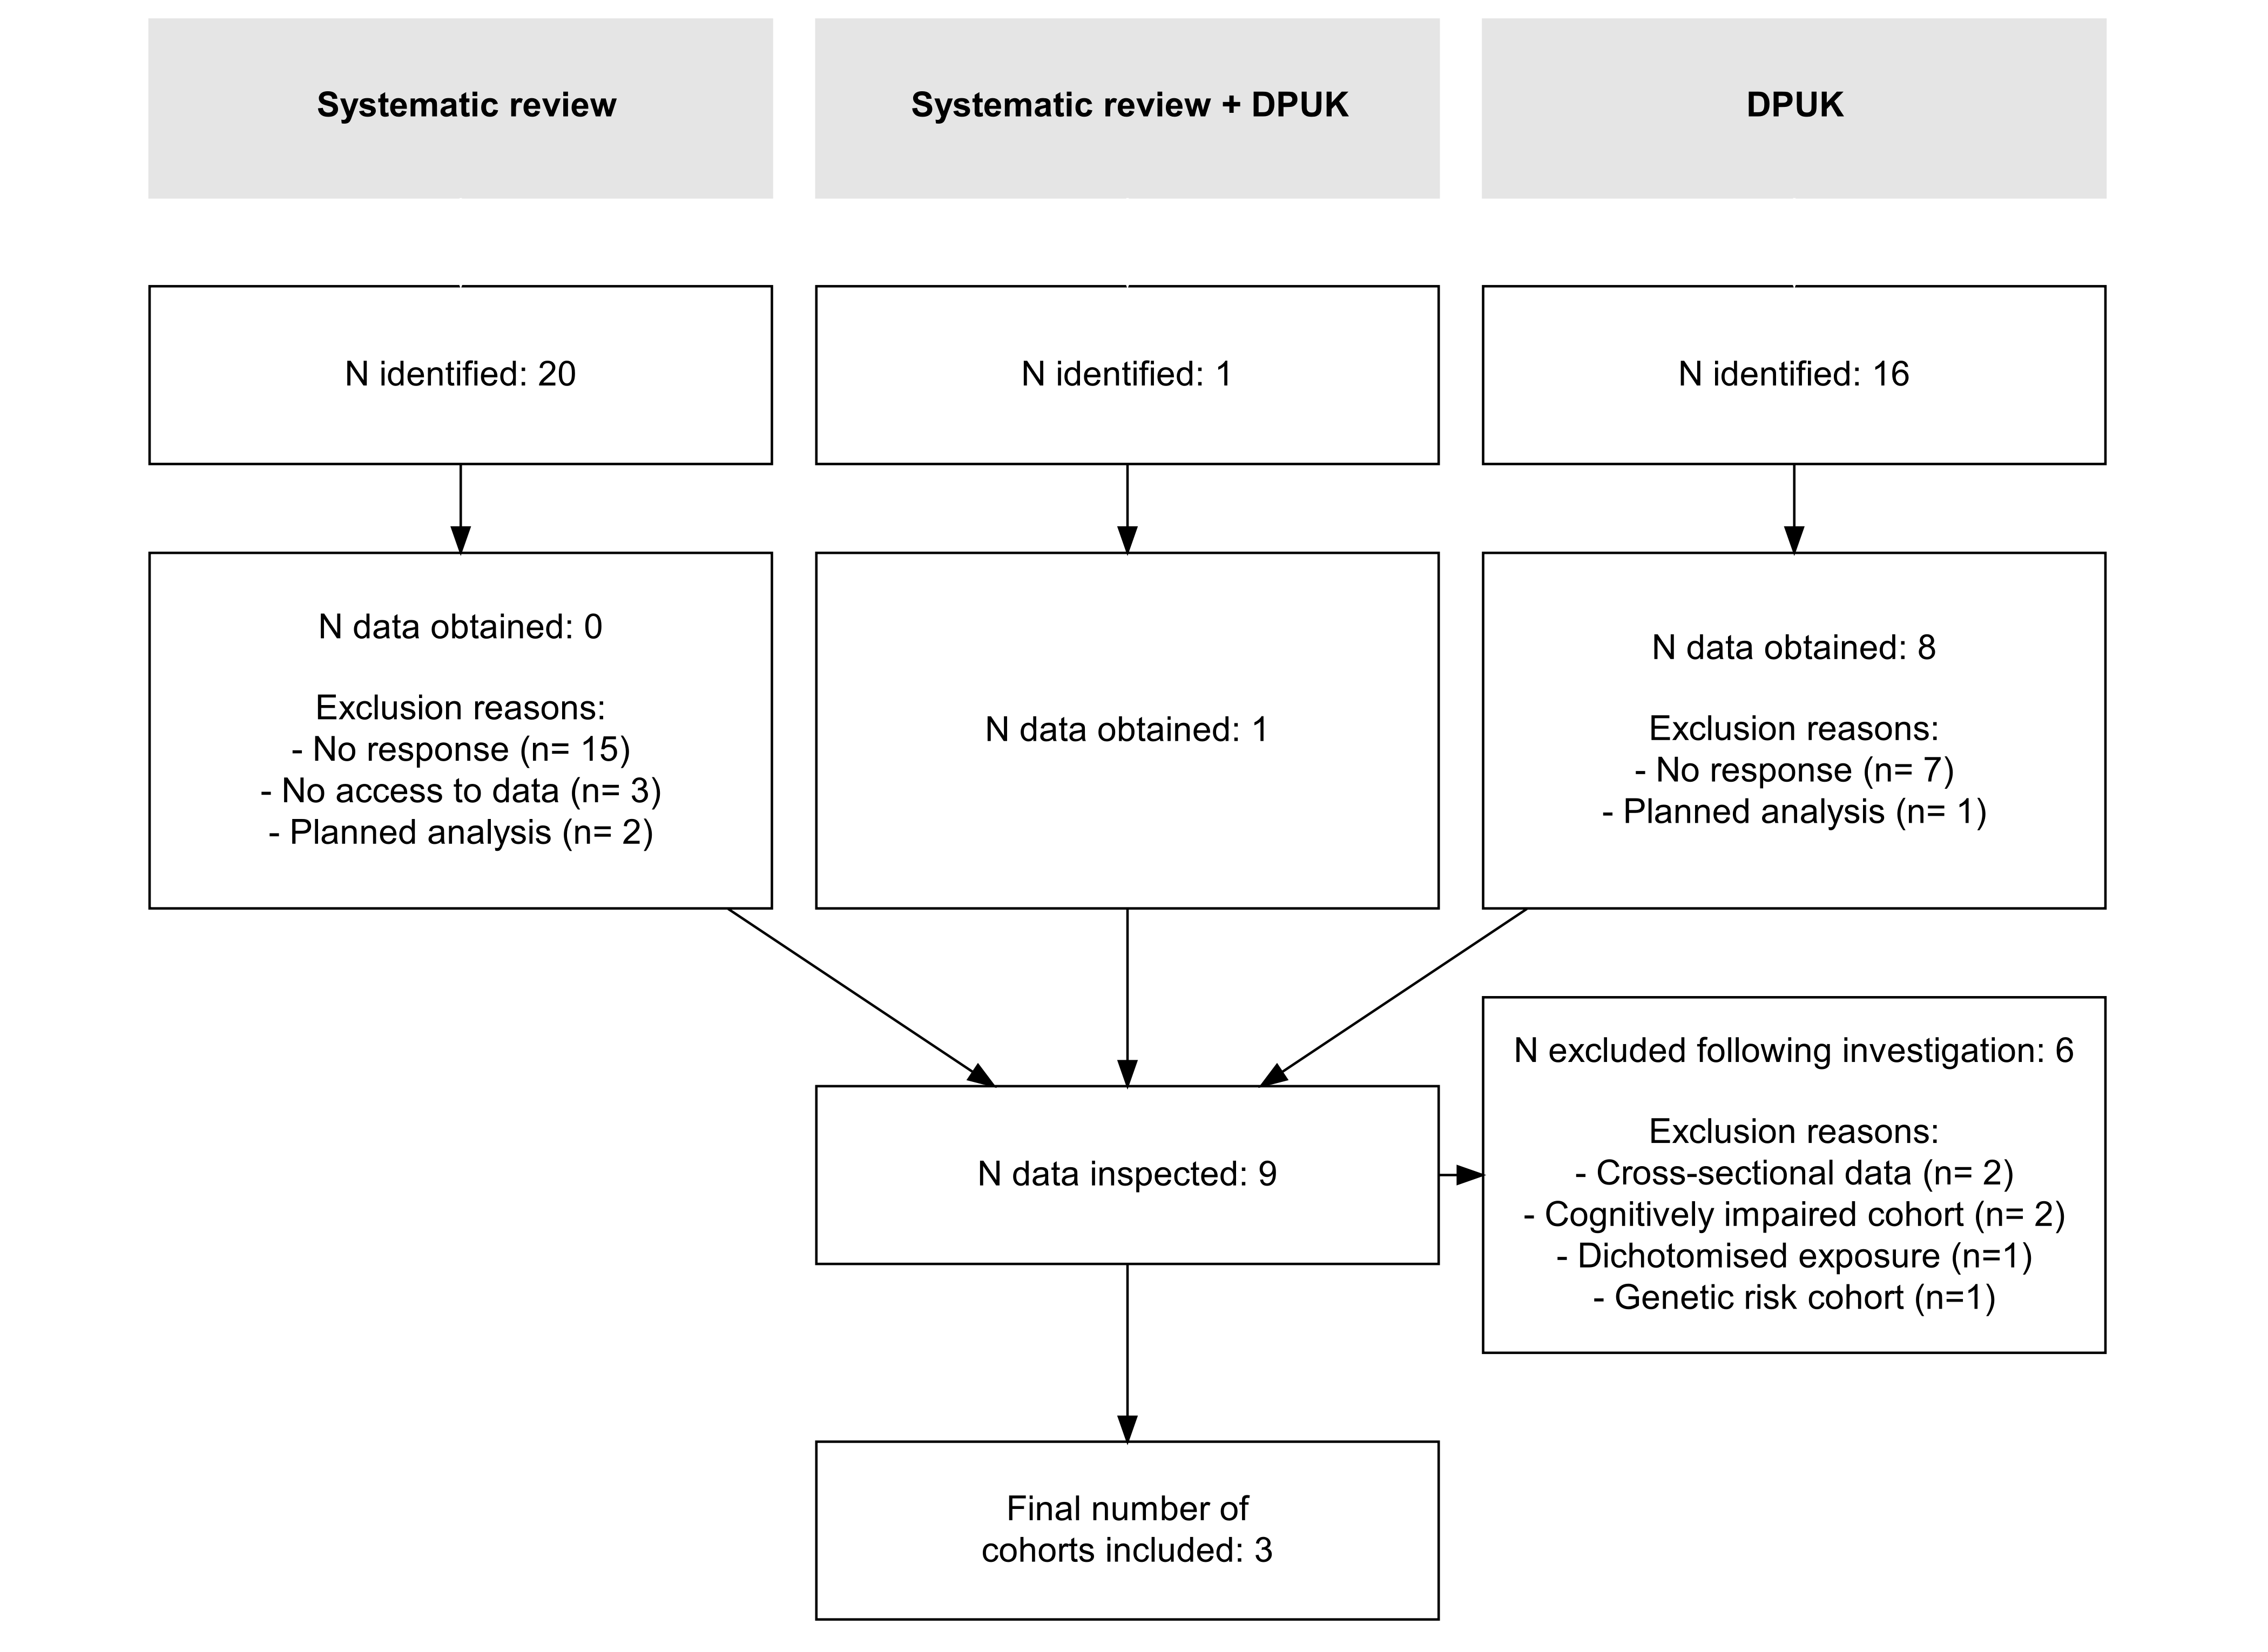
\includegraphics[width=1\linewidth]{figures/ipd/cohortFlowchart} \caption[Flowchart]{Flowchart of included cohorts, stratified by identification method (systematic review vs DPUK).}\label{fig:cohortFlowchart}
\end{figure}

As highlighted in Figure \ref{fig:cohortFlowchart}, there was little overlap between cohorts identified by the systematic review and those contained in the DPUK (n = 1, 2.7\%), indicating that the DPUK is a useful source of unanalysed data with respect to this question.

~

\hypertarget{included-data-sources}{%
\subsection{Included data sources}\label{included-data-sources}}

The four data sources used in this analysis are summarised in Table \ref{tab:cohortOverview-table} and are described in detail in the following sections. Of note, all included data sources were based in the United Kingdom. This is likely due to the majority of included datasets coming from the Dementia Platform UK route (Figure \ref{fig:cohortFlowchart}), which as implied by the name, has a geographical focus on cohorts performed in the United Kingdom.\textsuperscript{\protect\hyperlink{ref-bauermeister2020}{99}}

~





\begin{table}[H]

\caption[Summary of included cohorts]{\label{tab:cohortOverview-table}Summary of cohorts for which data were available}
\centering
\begin{tabular}[t]{>{\raggedright\arraybackslash}p{7em}>{\centering\arraybackslash}p{6em}>{\centering\arraybackslash}p{6em}>{\centering\arraybackslash}p{6em}>{\centering\arraybackslash}p{6em}}
\toprule
\textbf{Cohort} & \textbf{N} & \textbf{Dementia events (all-cause)} & \textbf{Age (mean)} & \textbf{Male (\%)}\\
\midrule
CaPS & 2512 & 1034 & 52 & 100\\
CPRD & X & X & X & X\\
EPIC & 1001 & 5 & 52 & 45\\
Whitehall II & 8022 & 181 & 50 & 69\\
\bottomrule
\end{tabular}
\end{table}

~

~

\hypertarget{caerphilly-prospective-study}{%
\subsubsection{Caerphilly Prospective Study}\label{caerphilly-prospective-study}}

The Caerphilly Prospective Study is a longitudinal study of men in the

Cholesterol measures (total, LDL-c, HDL-c and triglyceride) were measured at baseline in 1979-1983.
As the study population has aged, additional outcomes. Of particular relevance to this analysis, from Phase III (1989-1993) onwards, a battery of cognitive tests were introduced.

~

\hypertarget{cprd}{%
\subsubsection{CPRD}\label{cprd}}

The Clinical Practice Research Datalink (CPRD) is a large population-based, electronic health record (EHR) database.\textsuperscript{\protect\hyperlink{ref-herrett2015}{265}} containing the primary care records for more than 10 million primary care patients in England, and is broadly representative of the UK population in terms of age, sex and ethnicity.\textsuperscript{\protect\hyperlink{ref-herrett2015}{265},\protect\hyperlink{ref-mathur2014}{268}}

The CPRD is introduced more fully in Chapter @ref(). Briefly, a similar approach to the cohort definition as used in Chapter

Participants were included from the first date of lipid measurement, so no issues with immortal time bias as discussed in Chapter \ldots{}

Additionally, other number of participants is larger in this analysis as there is no restriction on the level which lipids should be in order to be included in the analysis.

the

~

\hypertarget{epic-norfolk}{%
\subsubsection{Epic Norfolk}\label{epic-norfolk}}

The European Prospective Investigation of Cancer - Norfolk is a\textsuperscript{\protect\hyperlink{ref-riboli1997}{307},\protect\hyperlink{ref-riboli2002}{308}}

The added evidental value of the EPIC cohort is small, given the relatively small number of participants and the fact that the cohort has only 8 dementia events.

~

\hypertarget{whitehall-ii}{%
\subsubsection{Whitehall II}\label{whitehall-ii}}

\emph{The Whitehall II study is a prospective cohort study of 10 308 participants (70\% men), aged 35--55 years and recruited between 1985 and 1989 from 20 London-based Civil service departments (\url{https://www.ucl.ac.uk/whitehallII}). Clinical examinations have been performed in 1991-1994, 1997-1999, 2002-2004, 2007-2009, 2012-2013, 2015-2016 with the data from circulating metabolomic traits and cognitive testing for the present study obtained from the 1997-1999 clinic phase.} - taken from EN ID: 2140

This data source was analysed in one of the included studies identified by the systematic review presented in Chapter \ref{sys-rev-heading},\textsuperscript{\protect\hyperlink{ref-tynkkynen2018}{221}} meaning that a comparison between the published result and the analysis reported here was was possible.

~

\hypertarget{excluded-data-sources}{%
\subsection{Excluded data sources}\label{excluded-data-sources}}

\hypertarget{cohorts-identified-the-systematic-review-but-excluded-from-the-ipd-analysis}{%
\subsubsection{Cohorts identified the systematic review but excluded from the IPD analysis}\label{cohorts-identified-the-systematic-review-but-excluded-from-the-ipd-analysis}}

The main reason for exclusion within this records was use of an electronic health record database. Examples included the Taiwan National Health Insurance database and studies run in the US making use of Medicare data.

~

\hypertarget{cohorts-identified-in-the-dpuk-but-excluded-from-the-ipd-analysis}{%
\subsubsection{Cohorts identified in the DPUK but excluded from the IPD analysis}\label{cohorts-identified-in-the-dpuk-but-excluded-from-the-ipd-analysis}}

Several additional cohorts are present in the DPUK collection but were not formally approached with a request for data access. This was primarily due to the information obtained via the online data dictionary system or via initial contact with the cohort owners indicating that the study was relatively new (and so was yet to collect more than 1 wave of data) or that the exposure variables of interest were not recorded.

~

\hypertarget{cohorts-providing-data-but-ultimately-excluded}{%
\subsubsection{Cohorts providing data but ultimately excluded}\label{cohorts-providing-data-but-ultimately-excluded}}

As highlighted in Figure \ref{fig:cohortFlowchart}, several cohorts from the DPUK responding positively but on inspection of data provided these cohorts were excluded for a range of reason. The exclusion reason for each cohort for which data were provided is illustrated in Table \ref{tab:dataExcluded-table}.

~





"``,''Cohort``,''Reason"
``1'',``NICOLA'',``Cross-sectional - only one wave of data available''
``2'',``TRACK HD'',``Participants carried HTT gene (i.e.~premanifest Huntington's Disease). Cohort owners indicated that this is likely to overshadw''

\begin{table}[H]

\caption[Exclusion reasons for cohorts providing data]{\label{tab:dataExcluded-table}Exclusion reasons for cohorts providing data}
\centering
\begin{tabular}[t]{>{\raggedright\arraybackslash}p{7em}>{\raggedright\arraybackslash}p{24em}}
\toprule
\textbf{Cohort} & \textbf{Reason}\\
\midrule
NICOLA & Cross-sectional - only one wave of data available\\
TRACK HD & Participants carried HTT gene (i.e. premanifest Huntington's Disease). Cohort owners indicated that this is likely to overshadw\\
\bottomrule
\end{tabular}
\end{table}

~

BRACE is a memory-complaint-based cohort, suggesting that it is unlikely they were dementia-free at baseline). Similarly, the Memento study was excluded as it's criteria for entry required participants to be outpatients from a memory clinic. The Generation Scotland provided only cross-sectional data only for the variables of interest, as did the the NICOLA study. Finally, the ELSA study was excluded based on the definition of the exposure variable. This study provided a ``high cholesterol'' a binary variable rather than the raw continuous lipid measurement data.

~

\hypertarget{cohorts-approach-but-received-no-answer}{%
\subsubsection{Cohorts approach but received no answer}\label{cohorts-approach-but-received-no-answer}}

This was particularly common among the cohorts identified via the systematic review and included studies with a dedicated access process or data access committee. A cohort of particular interest, having been used in multiple studies identified by the systematic review, is the Three City Study in France. Despite multiple attempts to contact the team, there was no response received. This study was approach at multiple points over the curse of this analysis, and no answer was received.

This was also a problem for cohorts approach via the DPUK - half of the cohorts applied to did not respond to the application within a year.

\hypertarget{analytical-results}{%
\subsection{Analytical results}\label{analytical-results}}

There was no evidence for an effect of any lipid fraction on any dementia outcome (Figure \ref{fig:tcDementiaMain}). Additionally, meta-analysis of the interaction coefficients for age-at-lipid-measurement and participant sex did not reveal an evidence for an varying effect across these variables.

~





\begin{figure}[H]
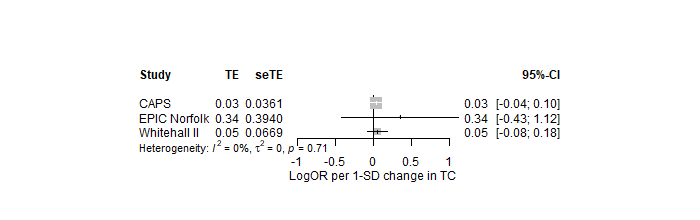
\includegraphics[width=1\linewidth]{figures/ipd/TC} \caption[IPD analysis of total cholesterol and dementia]{\textbf{Random effects meta-analysis of estimates from included data sources:}}\label{fig:tcDementiaMain}
\end{figure}

~

\hypertarget{discussion-3}{%
\section{Discussion}\label{discussion-3}}

\hypertarget{summary-of-findings-2}{%
\subsection{Summary of findings}\label{summary-of-findings-2}}

This analysis requested data from 37 data sources, but only obtained data from n = 3, 8.1\%, all of which were based in the United Kingdom. No evidence for an effect of lipids on the risk of dementia or related outcomes was identified. Similalarly, there was no evidence for an effect of age-at-measurement or sex on the lipid-dementia relationship.

Additionally analyses revealed that authors of cohorts indentified by the systematic review rarely stated that the data underpinning their analyses would be freely available, while a review of corresponding authors of these publications demonstrated that for many, the institutional email address provided was out of date.

\hypertarget{limitations-1}{%
\subsection{Limitations}\label{limitations-1}}

\hypertarget{low-response-rate-to-request-for-data}{%
\subsubsection{Low response rate to request for data}\label{low-response-rate-to-request-for-data}}

\emph{(although, in hindsight, the form of contact used (email) has been shown to be less successful in eliciting responses from authors when compared with telephoning\textsuperscript{\protect\hyperlink{ref-danko2019}{309}})}

A key limitation of this analysis is the very low response rate to requests for data access. This finding is not unexpected however, given that a review of IPD studies published between 1987 and 2015 found that fewer than half managed to obtained data from greater than 80\% of studies, and that in many cases, the exact percentage of studies for which data were obtained was not accurately reported.

There are likely several likely reasons for this low response rate. In general terms, there are a several well-documented reasons why data are not made readily available, including concerns regarding participant privacy, concerns around scoping or ``parasitic'' behaviour, and a lack of trust between primary and secondary researchers.

More specific to this analysis, individual participant data meta-analysis including studies other than randomised controlled trials have less success in obtaining individual participant data from studies.\textsuperscript{\protect\hyperlink{ref-nevitt2017a}{94}} Additionally, while no evidence is available on whether the characteristics of the researcher requesting data access influences the response rate and eventual decision, there is the possibility that my position as a PhD student meant I was less likely to elicit the response rate than a well-known professor might. The timing of the requests for data access, coinciding with a global pandemic, may also have affected the response rate as researchers prioritised other work.

\emph{Many authors claim that their data can be made ``available on request'', despite previous work establishing that these statements are demonstrably untrue in the majority of cases - that when data is requested, it is not actually made available.\textsuperscript{\protect\hyperlink{ref-krawczyk2012}{310}--\protect\hyperlink{ref-naudet2018}{312}} Additionally, previous work found that the availability of data ``available on request'' declines with article age, indicating that this approach is not a valid long term option for data sharing.\textsuperscript{\protect\hyperlink{ref-vines2014}{97}} Several of the included studies are greater than 10 years old, and so obtaining data from these cohorts is less likely compared with more recently published studies.}

One of the reasons for this may be that the email addresses reported on publications are more likely to be out of date for older publications. Qualitatively, investigation of a subset of cohorts revealed that several corresponding/first authors were no longer at the same institution as when the study was reported, and as a result, were unlikely to have access to the institutional email address listed on the study publication.

These challenges are in theory what the DPUK was built to address. However, even with the help of the streamlined application process afforded by the DPUK, accessing sufficient data was a challenge. The response rate among DPUK cohorts a year after application was just 50\%. In addition, some cohorts responded that that the proposed study question was already under investigation by another group, and that they would not share the data on this basis. In light of this, a centralised database of ongoing analysis being performed in DPUK would be of enormous help. Finally, the DPUK should more clearly distinguish between those cohorts that are ``DPUK native'' versus externally hosted, as the response time for externally hosted cohorts is likely to be much longer.

Whether or not to press ahead with an IPD analysis in the absence of all (or even most) data is a personal decision, and some previous analyses have highlighted where they decided not to pursue an IPD study.\textsuperscript{\protect\hyperlink{ref-jaspers2014}{313}}

For the purposes of this thesis, conducting the IPD analysis was useful as it afforded me the opportunity to gain experience in applying the methodology. In addition, it allowed me to analysed two addition previously unanalysed cohort studies which were then utilised in the triangulation study detailed in Chapter \ref{tri-heading}.

~

\hypertarget{risk-of-bias-assessment-1}{%
\subsubsection{Risk of bias assessment}\label{risk-of-bias-assessment-1}}

There is some concerns about performing risk of bias assessments on your own analysis, and so two secondary reviewers

~

\hypertarget{strengths-1}{%
\subsection{Strengths}\label{strengths-1}}

While this analysis did not manage to systematically obtain and analyse a large proportion of identified data, it did enable an analysis of two previously unanalysed datasets - the CaPS study and the EPIC Norfolk study - providing additional data that is incorporated into the triangulation exercise reported in Chapter \ref{tri-heading}.

~

~

\hypertarget{reflections-on-the-process}{%
\subsection{Reflections on the process}\label{reflections-on-the-process}}

In hindsight, attempting to undertake a large-scale IPD meta-analysis as part of a larger PhD project may have been overly ambitious. Data harmonization between cohorts in an IPD analysis is an often under-appreciated challenge,\textsuperscript{\protect\hyperlink{ref-levis2021}{303}} and in line with this, data cleaning for this analysis took substantially longer than expected.

~

\hypertarget{conclusion}{%
\section{Conclusion}\label{conclusion}}

This analysis provided very weak evidence for an effect of lipid fractions on dementia outcomes. However, it does provide an analysis two previous unanalysed data sources that are subsequently used in Chapter \ref{tri-heading}.

\newpage

\hypertarget{references-4}{%
\section{References}\label{references-4}}

\begin{savequote}
Next on my list of features to be specially considered I would place the
consistency of the observed association. Has it been repeatedly observed
by different persons, in different places, circumstances and times?
\qauthor{--- Sir Austin Bradford Hill, 1965\textsuperscript{\protect\hyperlink{ref-hill1965}{314}}}\end{savequote}



\hypertarget{tri-heading}{%
\chapter{Aetiological triangulation across new and existing evidence sources}\label{tri-heading}}

\minitoc 

\hypertarget{lay-summary-5}{%
\section{Lay summary}\label{lay-summary-5}}

\textbf{TBC}

~

\newpage

\newpage

\hypertarget{triangulation-overview}{%
\section{Introduction}\label{triangulation-overview}}

Aetiological triangulation, or simply triangulation, is the process of comparing and contrasting across different sources of evidence. Triangulation is broadly comparable to Bradford-Hill's criteria of ``consistency'', that is the replication of an observed relationship across several different contexts,\textsuperscript{\protect\hyperlink{ref-hill1965}{314}} where contexts are assumed to have different underlying bias structures. More formally it can be defined as:

\begin{quote}
The practice of strengthening causal inferences by integrating results from several different approaches, where each approach has different (and assumed to be largely unrelated) key sources of potential bias.\textsuperscript{\protect\hyperlink{ref-lawlor2016}{315}}
\end{quote}

This approach represents a significant step forward from the current evidence synthesis practice of synthesising evidence from only one approach (e.g.~randomised controlled trials (RCTs), non-randomised studies of exposures (NRSE) or interventions (NRSI), etc.). The most common implementation of this method to date has been in the form of \emph{qualitative triangulation} - that is the identification and a narrative comparison, where the internal biases and differences between the study question and the causal question of interest (indirectness) of each result are discussed.

However, qualitative triangulation faces issues at scale. There is a need to include all evidence, as otherwise the potential for cherry-picking, yet as the number as it is not possible to compare and contrast across multiple results in any meaningful way. This fact is also illustrated by previous exemplars of triangulation only considering three individual results. An alternative option previously employed is to assign bias to the output of a meta-analysis of similarly designed studies, but this loses information on the specific biases inherent to each results contributing to the summary estimate. For example, while it may be true that all non-randomised studies share some minimal level of bias, investigation of the biases applicable to each individual result gives useful additional information. Recent development in bias assessment have allowed for a much more granular consideration of the threats to the internal validity of a result. In combination, these limitations to qualitative triangulation detail a need for a more systematic way to integrate across multiple evidence sources as the number of individual results contributing to the exercise increases.

This chapter, in addition to providing a narrative comparison of the existing and new evidence identified in this thesis, builds on recent developments in risk-of-bias assessment and existing methods for bias-/indirectness-adjusted meta-analysis to propose a generalised framework for quantitative triangulation. The method, along with the methodological challenges to its implementation, is illustrated via a proof-of-concept case study examining the causal effect of average exposure to LDL-c at mid-life on Alzheimer's disease risk. In the following section, I define important terms used throughout this chapter.

~

\newpage

\hypertarget{tri-terminology}{%
\subsection{Terminology}\label{tri-terminology}}

For the sake of clarity, and given the multiple competiting defitions used to define key concepts on this topic, I begin by defining the terms as used in this chapter.

\textbf{Bias vs indirectness}

Both

Bias (or internal bias) in the result is defined as systematic deviation from result the ``idealised'' version of the study (that is, )

In contrast, the indirectness of the result (also called generalisability or applicability) is defined here as the discrepancy between the research question addressed by the ``idealised'' study and the causal question of interest. Problems with indirectness can be arise from differences in population, intervention/exposure, outcomes and

Of note, the original method employed in this chapter refers indirectness as ``external bias'' - however. This distinction is important, as bias and indirectness describe two different issues, and referring to both as bias

In addition, indirectness is the widely used term, including by widely-adopted methods such as the GRADE framework.\textsuperscript{\protect\hyperlink{ref-guyatt2011}{316}}

\textbf{Additive vs proportional effects}

Additive biases (identified by a ``Favours experimental''/``Favours comparator'' response) are XXXX. A key example of additive bias is immortal time bias, which will always favour the intervention.

Proportional biases (identified by a ``Towards null''/``Away from null'' response) are those related to the magnitude of the effect. A key example of this type of bias is non-differential misclassification bias, which will bias the effect estimate towards the null.

The effects of both bias and indirectness can be either additive or propotional.

Additive bias/indirectness is

Both bias and indirectness can be defined as additive or propotional. Additive bias/indirectness is that which can shift the p

~

\newpage

\hypertarget{methods-3}{%
\section{Methods}\label{methods-3}}

\hypertarget{tri-data-sources}{%
\subsection{Data sources}\label{tri-data-sources}}

This triangulation exercise draws on the research produced in each of the preceding chapters. More specifically, this chapter builds on the comprehensive systematic review presented in chapter \ref{sys-rev-heading}. It also incorporates the new evidence produced by the analysis of the association of statin use with dementia outcomes in the CPRD (Chapter \ref{cprd-heading}) and of the association of lipids with dementia outcomes in previously unanalysed datasets accesssed via the DPUK (Chapter \ref{ipd-heading}).

Table \ref{tab:thesisOverview-table} summarises the research each approach has attempted to address, the exposures and outcomes considered in each study, and the contribution of each chapter to the triangulation exercise presented here.

\blandscape





\begin{table}[H]

\caption[Summary of research designs included in this thesis]{\label{tab:thesisOverview-table}Summary of studies included in this thesis, and used as evidence sources in this triangulation exercise. Note, Chapter \ref{sys-rev-tools-heading} is intentionally not included in this table, as it describes a research tool rather than a research study.}
\centering
\begin{tabular}[t]{>{\raggedright\arraybackslash}p{6em}>{\raggedright\arraybackslash}p{16em}>{\raggedright\arraybackslash}p{7em}>{\raggedright\arraybackslash}p{7em}>{\raggedright\arraybackslash}p{16em}}
\toprule
\textbf{Chapter} & \textbf{Research Question} & \textbf{Exposure/ Intervention} & \textbf{Outcome} & \textbf{Contibution to evidence synthesis framework}\\
\midrule
Chapter 3/4 & Based on the available evidence; \newline (i) are lipid fractions associated with subsequent dementia risk, stratified by subtype? \newline (ii) Are lipid regulating agents associated with subsequent dementia risk, stratified by subtype? \newline & Lipids (HDL-c, LDL-c, TC, TG), \newline \newline Lipid regulating agents (statins, ezetimibe, fibrates, etc.) & Dementia, stratified by subtype & Provides overview of existing evidence, including detailed risk-of-bias assessments for each result\\
\midrule
Chapter 5 & Are lipid regulating agents associated with dementia risk in a large scale electonic health record database? \newline & Seven classes of lipid regulating agents & Dementia, stratified by subtype & Provides additional observational data on vascular dementia (under-represented in the literature) \newline \newline Provides a source of observational evidence created using a method with distinct sources of bias to those identified by the systematic review\\
\midrule
Chapter 6 & Are lipid levels associated with dementia risk in an individual participant data meta-analysis? \newline & Lipids (HDL-c, LDL-c, TC, TG) & Dementia, stratified by subtype & Provides additional evidence from unanalysed datasets\\
\bottomrule
\end{tabular}
\end{table}

\elandscape

\hypertarget{qualitative-triangulation}{%
\subsection{Qualitative triangulation}\label{qualitative-triangulation}}

As discussed in the introduction to this Chapter (Section \ref{triangulation-overview}), as part of a narrative synthesis of the evidence all information sources were grouped by outcome, and systematically compared and contrasted. Potential reasons for heterogeneity between study designs were examined with specific reference to the risk-of-bias assessments performed.

This analysis built on the detailed risk of bias assessments performed and presented as part of the systematic review (Chapter @ref()/@ref()). Similarly, risk-of-bias assessments were performed for each new source of evidence presented in this thesis, details of which are available in Appendix @ref(?).

~

\hypertarget{quantitative-triangulation}{%
\subsection{Quantitative triangulation}\label{quantitative-triangulation}}

In addition to the qualitative discussion of evidence, I attempted to integrate the numerical results of the multiple approaches. This proof-of-concept approach incorporates recent advancements in the way that bias in results is assessed (move from checklists to domain-based assessment tools)\textsuperscript{\protect\hyperlink{ref-sterne2019}{145}} and existing methods for bias-/indirectness-adjusted meta-analysis\textsuperscript{\protect\hyperlink{ref-turner2009}{317}} to to illustrate how causal questions could be addressed under this quantitative triangulation framework.

This proposed framework involves several steps, as described in detail in the following sections. In summary these steps are:

\begin{enumerate}
\def\labelenumi{\arabic{enumi}.}
\tightlist
\item
  Define the causal question of interest
\item
  Identify of relevant evidence sources and standardisation of effect directions
\item
  Assess and visualise the extent and direction of bias in each result
\item
  Define modifying terms for bias and indirectness in each result
\item
  Caclulate bias-/indirectness-adjusted results and perform meta-analysis
\end{enumerate}

In order to illustrate the bias-/indirectness adjustment process detailed in the subsequent sections, the process for calculating the adjusted estimate for a single study is described in detail for a single study. Following this, the process for an example causal question as a case study, as defined below.

~

\hypertarget{definition-of-the-causal-questions-of-interest-case-studies}{%
\subsubsection{Definition of the causal questions of interest (case-studies)}\label{definition-of-the-causal-questions-of-interest-case-studies}}

Given that this quantitative analysis is intended as a proof-of-concept for the framework, rather than aiming to produce findings that should guide clinical practice, I consider only one of the multiple possible causal questions related to the broad topic of the effect of lipids on dementia outcomes.

Using the ROBINS-E framework I defined the parameters of my causal question of interest:

\begin{itemize}
\tightlist
\item
  \emph{Population of interest}: General population
\item
  \emph{Exposure of interest}: Low density lipoprotein cholesterol
\item
  \emph{Exposure window of interest}: Mid-life (45-60)
\item
  \emph{Summary measure of exposure over time}: Average exposure
\end{itemize}

This question was chosen for a number of reason. Firstly, given the long prodomal period between the onset of physiological changes in the brain and presentation of dementia symptoms, it seems likely that conditions during the mid-life period is particularly important. Secondly, examining the causal impact of lipids on a specific outcome (in this case, Alzheimer's disease), rather than a composite outcome (all-cause dementia), focuses on an single causal pathway rather than including conditions that likely have very different mechanisms of disease. Finally, and relevant to its use as a case study for the quantitative triangulation approach, this question had several relevant sources of evidence available (versus, for example, any question looking at vascular dementia).

~

\hypertarget{identify-relevant-studies}{%
\subsubsection{Identify relevant studies}\label{identify-relevant-studies}}

Once the causal question of interest had been defined, relevant individual results were obtained from the data sources described in Section \ref{tri-data-sources}. In a broad sense, this meant pulling out studies that examined the relationship between LDL-c and Alzheimer's disease risk, either directly (non-randomised studies of LDL-c levels) or indirectly (non-randomised studies of statins, Mendelian randomisation studies using genetic instruments for LDL-c levels).

Once the set of relevant results were identified, effects were standardised to refer to the risk of Alzheimer's disease resulting from a ``reduction'' in LDL-c.~For studies of statins, th. However, for both non-randomised studies and Mendelian randomisation analysis of lipid levels, the effect is usually reported per 1-SD increase in LDL-c.~In this case, the effect estimates were inverted to ensure consistency across study designs.

~

\hypertarget{assess-risk-and-direction-of-bias-in-each-result}{%
\subsubsection{Assess risk and direction of bias in each result}\label{assess-risk-and-direction-of-bias-in-each-result}}

The risk of bias tools used to assess each result are described in detail in Section \ref{risk-of-bias}. In summary, RTCS were assessed using the RoB 2 tool;\textsuperscript{\protect\hyperlink{ref-sterne2019}{145}} NRSI using the ROBINS-I tool;\textsuperscript{\protect\hyperlink{ref-sterne2016}{142}} NRSE using the ROBINS-E tool (see Section @ref(\#rob-tools-nrse));\textsuperscript{\protect\hyperlink{ref-morganr2020}{146},\protect\hyperlink{ref-french2019}{147}} and MR studies using the Mamluk et al.~tool.\textsuperscript{\protect\hyperlink{ref-mamluk2020}{149}}

For the sake of consistency, I mapped the different acceptable judgements in each risk-of-bias tool to a harmonised set of judgements: ``Low'', ``Moderate'',``High''. The exact mapping can be seen in Table \ref{tab:robLevelsMapping-table}. Of note, no mapping was performed for the critical risk-of-bias levels present in the tools for non-randomised studies. This is because current best practice in evidence synthesis is to exclude all studies at critical risk of bias for further quantitative synthesis.\textsuperscript{\protect\hyperlink{ref-sterne2016}{142}}

~\\




\begin{table}[H]

\caption[robLevelsMapping]{\label{tab:robLevelsMapping-table}robLevelsMapping}
\centering
\begin{tabular}[t]{>{}cccc}
\toprule
\textbf{Harmonised} & \textbf{RoB2} & \textbf{ROBINS-I / ROBINS-E} & \textbf{MR}\\
\midrule
\textbf{Low} & Low & Low & Low\\
\midrule
\textbf{Moderate} & Some concerns & Moderate & Moderate\\
\midrule
\textbf{High} & High & Serious & High\\
\midrule
\textbf{-} & - & Critical & -\\
\bottomrule
\end{tabular}
\end{table}

~

In addition to assessing the extent of bias in each domain, as defined by the three levels detailed above, I attempted to record the predicted direction and type of bias. This was achieved via an additional question at the end of each bias domain, which asked assessors to predict the expected direction of bias in that domain. Note that this question is currently only formally included in two existing tools (ROB2/ROBINS-I), but I employed an identical approach during assessment of non-randomised studies of exposure and Mendelian randomisation studies. Acceptable responses to this question included:

\begin{itemize}
\tightlist
\item
  ``Favours experimental''/``Favours comparator'' (defines an additive bias)
\item
  ``Towards null''/``Away from null'' (defines a proportional bias)
\item
  ``Unpredictable''
\end{itemize}

As indicated in the options above, the response to this question is also used to determine the predicted type of bias (additive or proportional - see Section \ref{tri-terminology}) in addition to the direction. For additive biases, determining the absolute direction of bias was simply a case of whether the bias shift the effect estimate to the left or right on an imaginary forest plot. For example, if a bias was predicted to favour the intervention, then the estimate would be shifted to the right.

In contrast, for proportional biases, whether the estimate should be increased or decreased proportionally depends on the current position of the point estimate relative to the null. For example, if the effect estimate represents a protective effect (below the null), then bias towards the null would be adjusted for by moving the effect estimate propotionally to the right. In contrast, if the effect of the intervention is harmful (effect estimate above the null), bias towards the null would be adjusted for by moving the effect estimate propotionally to the left.





pdf
2

Note that for some domains, only one type of bias is allowed. For example, in the confounding domains in the ROBINS-I/ROBINS-E tools, only the ``Favours experimental''/``Favours comparator'', and ``Unpredictable'' options are available, meaning that bias in this domain will always be considered additive. Additionally, the predicted direction and type of bias were not recorded for domains at ``Low'' risk of bias.

~

\hypertarget{visualisation-of-extent-and-direction-of-bias}{%
\subsubsection{Visualisation of extent and direction of bias}\label{visualisation-of-extent-and-direction-of-bias}}

To aid with the triangulation exercise and to act as a sense-check, I created a new method to visualise the extent, direction and type of bias in each result to enable detailed comparison across different studies contributing to a synthesis. Similar to the standard paired forest plots introduced in Chapter \ref{sys-rev-}, these ``bias direction'' plots show the level of bias across the domains in each study is reported using coloured blocks. However, in contrast to the previous plots, symbols are used to illustrate the predicted absolute direction of bias in that domain, as discussed in the previous section. Distinct symbol pairs are used to denote additive and proportional biases.

Convience functions in the \texttt{triangulate} package (see Section \ref{tri-software}) were used to preprocess risk of bias data for use with both bias-direction plots and adjusted meta-analyses, as discussed in subsequent sections. These bias direction plots themselves were created using the risk-of-bias visualisation tool described in Appendix \ref(?).

~

\hypertarget{assign-modifying-values-to-riskdirection-of-bias}{%
\subsubsection{Assign modifying values to risk/direction of bias}\label{assign-modifying-values-to-riskdirection-of-bias}}

Following definition of the extent, type and direction of bias in each domain, I assigned a prior distribution on the log scale to each combination. For example, a ``high'' additive bias in \(j\)th domain of the \(i\)th study is deifined as \(\delta_{i,j}^{\mathrm{High}}\) and uncertainty around this estimate is given by a distribution:

\begin{equation}
  \delta_{i,j}^{\mathrm{High}} = f(\mu_{i,j}^{\mathrm{High}}, \sigma_{i,j}^{\mathrm{High}})
  \label{eq:name}
\end{equation}

The sign of \(\mu_{i,j}^{\mathrm{High}}\) is defined by the absolute direction of the bias. If the bias is expected to pull the effect to the left, the position is given a negative sign, and if it is expected to pull the effect to the right, it is given a positive sign.

One key feature of the domain-based risk-of-bias domains is that the domains are considered interchangeable - i.e.~a ``high'' judgement in one domain is equivalent to a ``high'' judgement in any other. As such, for this analysis, I assumed that the distributions assigned to each level of bias are identical across all values of \(j\), that is, are identical for all domains in the risk of bias assessment tool. To illustrate, for additive biases these means:

\[
\delta_{i,1}^{\mathrm{High}} = \delta_{i,2}^{\mathrm{High}} = ... = \delta_{i,j}^{\mathrm{High}}
\]

and similarly

\[
\delta_{i,1}^{\mathrm{Moderate}} = \delta_{i,2}^{\mathrm{Moderate}} = ... = \delta_{i,j}^{\mathrm{Moderate}}
\]

Reasonable values for the position and spread of the prior distributions were informed by a previous reported expert bias elicitation exercise.\textsuperscript{\protect\hyperlink{ref-turner2009}{317}} Using open data from that study, I calculated the mean and maximum values for the mean and variance of the adjustment distributions across all biases considered by that exercise (see Appendix @ref(?) for more details on how these were calculated). For the purposes of this illustrative analysis and to highlight the generalised nature of the code used to perform the analysis (see Section \ref{tri-software}), I used the calculated values to inform two sets of modifying distributions (Table \ref{tab:priorsAdd-table}) for additive biases, and a single set for proportional biases. In the first scenario, the relationship between the position assigned to each additive judgement is linear. In the second scenario, the step from ``moderate'' to high" is twice that from ``low'' to ``moderate''. Across both additive and proportional biases, the variance of the ``high'' risk--of-bias judgement distribution was defined to be greater than that for the ``moderate'' risk-of-bias judgement.

~





\begin{table}[H]

\caption[Additive bias distributions]{\label{tab:priorsAdd-table}Prior distributions for extent and type of bias under two scenarios, on the log scale. Note that the distributions for proportional biases were kept consistent across the two scenarios.}
\centering
\begin{tabular}[t]{>{}lccc}
\toprule
\multicolumn{1}{c}{\textbf{ }} & \multicolumn{2}{c}{\textbf{Additive bias}} & \multicolumn{1}{c}{\textbf{ }} \\
\cmidrule(l{3pt}r{3pt}){2-3}
\textbf{Bias Level} & \textbf{Scenario 1} & \textbf{Scenario 2} & \textbf{Proportional bias}\\
\midrule
\textbf{Low} & - & - & -\\
\midrule
\textbf{Moderate} & N(.08, .05) & N(.08, .05) & N(.03, .16)\\
\midrule
\textbf{High} & N(.16, .12) & N(.4, .29) & N(.1, .05)\\
\bottomrule
\end{tabular}
\end{table}

~

Where the direction of bias in a domain was unpredictable for a given result, the mean of the adjustment distribution for that domain was set to 0 but the appropriate variance for the recorded extent of bias was retained. In other words, adjusting for bias in a domain with an unpredictable direction of bias has no impact on the position of the effect estimate, but does increase uncertainty around it.

~

\hypertarget{assessing-and-assigning-modifying-values-to-indirectness}{%
\subsubsection{Assessing and assigning modifying values to indirectness}\label{assessing-and-assigning-modifying-values-to-indirectness}}

An identical approach was employed to assess and assign prior distributions to the risk of indirectness in each result. The target question for each result was compared against the causal question of interest with respect to three domains (population, intervention/exposure, outcome), again using the scale of ``Low/''Moderate``/''High" to quantify the extent of indirectness.

A similar approach was used to define prior distributions for external bias or indirectness. I used a similar enforced scale of ``Low/''Moderate``/''High" indirectness versus each of the 4 aspects of the target causal question. (recap). All indirectness were defined \emph{a priori} as being proportional in nature, in line with previous work on this topic.\textsuperscript{\protect\hyperlink{ref-turner2009}{317}}

As crude illustrative example, consider the causal question of the interest in this exercise, the effect of LDL-c in mid-life on Alzheimer's disease. Here, studies of lipids levels in this time period would require minimal adjustment, whereas studies examining statin use (indirect exposure/intervention) in late-life (indirect population) would be downweighted due to reduced relevance to the causal question.

~

\hypertarget{combine-in-a-bias-adjusted-meta-analysis}{%
\subsubsection{Combine in a bias-adjusted meta-analysis}\label{combine-in-a-bias-adjusted-meta-analysis}}

As per the method reported in, total additive and proportional bias and indirectness were calculated for each result. Briefly,

Once the total additive and proportional bias and indirectness for each result were computed, they were used to define an adjusted estimate for each result included in the synthesis.

Using the method defined in Turner \emph{et al},\textsuperscript{\protect\hyperlink{ref-turner2009}{317}} the adjusted estimate for each result, \(\hat\theta\), is defined as:

\begin{equation}
  \hat{\theta} = \frac{y_i - \mu_{i\beta}^{\mathrm{In}}\mu_{i\delta}^{\mathrm{In}} - \mu_{i\delta}^{\mathrm{B}}}{\mu_{i\beta}^{\mathrm{B}}\mu_{i\beta}^{\mathrm{In}}}
  \label{eq:adjusted-mean}
\end{equation}

The standard error of this estimate is then calculated as:

\begin{equation}
  \mathrm{SE}(\hat{\theta})=\left(\frac{1}{\mu_{i \beta}^{\mathrm{B}} \mu_{i \beta}^{\mathrm{In}}}\right)^{2}\left(s_{i}^{2}+\left(\mu_{i \beta}^{\mathrm{B}} 2+\sigma_{i \beta}^{\mathrm{B}}\right)\left(\hat{\theta}^{2} \sigma_{i \beta}^{\mathrm{In} 2}+\sigma_{i \delta}^{\mathrm{In} 2}\right)+\sigma_{i \beta}^{\mathrm{B}}\left(\hat{\theta} \mu_{i \beta}^{\mathrm{In}}+\mu_{i \delta}^{\mathrm{In}}\right)^{2}+\sigma_{i \delta}^{\mathrm{B} 2}\right)
  \label{eq:adjusted-se}
\end{equation}

Once each individual result has been adjusted, I performed a random effects meta-analysis using the unadjusted and adjusted (under the two scenarios defined above) results.

~

\hypertarget{results-3}{%
\section{Results}\label{results-3}}

\hypertarget{qualitative-triangulation-1}{%
\subsection{Qualitative triangulation}\label{qualitative-triangulation-1}}

\hypertarget{all-cause-dementia}{%
\subsubsection{All-cause dementia}\label{all-cause-dementia}}

\textbf{Statins and all-cause dementia}

This conflicts with the findings of our analysis, where statin use was associated with an increased risk of all-cause dementia (HR:1.17, 95\%CI:1.14-1.19). Some of the included studies in the meta-analysis specifically exclude vascular dementia from the definition of all-cause dementia,\textsuperscript{\protect\hyperlink{ref-chao2015}{318}} which may limit the ability for comparison with our findings for the all-cause dementia outcome.

Additionally, a previous analysis of the THIN EHR database using a propensity-score matched analysis found a protective effect of statins on all-cause dementia (HR:0.81, 95\%CI:0.69-0.96)\textsuperscript{\protect\hyperlink{ref-smeeth2009}{292}}.

~

\hypertarget{alzheimers-disease}{%
\subsubsection{Alzheimer's disease}\label{alzheimers-disease}}

\textbf{Statins and Alzheimer's disease}

Our results are broadly in line with the findings of two distinct approaches examining the effect of statin treatment on subsequent Alzheimer's disease. No randomized trials of statins for the prevention of Alzheimer's disease have been reported, but a recent meta-analysis of 20 observational studies found statins were associated with a reduced risk of Alzheimer's disease (RR 0.69, 95\% CI 0.60--0.80) with stronger evidence than observed in our analysis.\textsuperscript{\protect\hyperlink{ref-poly2020}{243}} This review included case-control studies and analyses likely to be at risk of immortal time bias, which may account for the discrepancy with our findings. Additionally, a recent Mendelian randomization study examining the effect of genetic inhibition of HMGCR on Alzheimer's disease (a genetic proxy for statin treatment) provided equivocal evidence (OR: 0.91, 95\%CI: 0.63-1.31) but was consistent with our results.\textsuperscript{\protect\hyperlink{ref-williams2020}{319}}

Our additional analyses stratified by statin properties found little evidence of differences in associations of lipophilic and hydrophilic statins and incidence of Alzheimer's disease, consistent with a recent meta-analysis of observational studies.\textsuperscript{\protect\hyperlink{ref-chu2018}{57}}

~

\hypertarget{vascular-dementia}{%
\subsubsection{Vascular dementia}\label{vascular-dementia}}

\textbf{Statins and vascular/other dementia}

Far fewer studies have tested the association between lipid-regulating agents and vascular dementia or other dementias. A recent review found four observational studies examining the association of statins and vascular dementia found limited evidence for an effect (RR:0.93, 95\% CI 0.74--1.16).\textsuperscript{\protect\hyperlink{ref-poly2020}{243}} This contrasts with the harmful association found in our analysis (HR:1.81, 95\%CI:1.73-1.89). When stratifying by lipid properties, lipophilic statins were more harmful than hydrophilic statins in vascular dementia, potentially due to their ability to cross the blood brain barrier.

~

\textbf{Other drug classes}

Apart from statins, few studies examining a lipid-regulating agent have been reported (Chapter \ref{sys-rev-methods-heading}/\ref{sys-rev-results-heading}).

One of the few classes for which a evidence was available were fibrates, which found little evidence of an association with all-cause dementia was identified,\textsuperscript{\protect\hyperlink{ref-ancelin2012}{158}} inconsistent with our finding that patients prescribed fibrates had higher all-cause dementia risk than those prescribed other lipid lowering agents.

A previous Mendelian randomization study found little evidence that genetic variants that proxy for ezetimibe affect risk of Alzheimer's disease (OR: 1.17, 95\%CI: 0.73-1.87),\textsuperscript{\protect\hyperlink{ref-williams2020}{319}} consistent with our findings. Note that this study was published in 2020 and so was not included in the review.

~

\hypertarget{quantitative-triangulation-1}{%
\subsection{Quantitative triangulation}\label{quantitative-triangulation-1}}

\hypertarget{single-study}{%
\subsubsection{Single study}\label{single-study}}

Explain how example study was chosen

Show result and bias

Reproduce version of Table 2 rom the ``proposed method'' paper for indirectness

Total additive bias (on the log scale) was \textbf{PLACEHOLDER}. Similarly, total additive indirectness was (),

Calculate internal-bias adjusted

\textbf{PLACEHOLDER}

The unadjusted effect for this study was \textbf{PLACEHOLDER} and the adjusted effect estimate for this study was \textbf{PLACEHOLDER}





\begin{figure}[H]

\includegraphics[width=1\linewidth]{figures/misc/UoBcrest} \caption[Bias direction plot for a single study]{Bias direction plot for a single study showing the predicted direction of bias in each domain. Additive biases are characterised using arrows, while the proportional biases are denoted using \(<\) and \(>\). A question mark indicates that the direction of bias was unpredictable.}\label{fig:biasDirectionSingle}
\end{figure}

~

\hypertarget{case-study-effect-of-ldl-c-at-midlife-on-alzheimers-disease}{%
\subsubsection{Case study: effect of LDL-c at midlife on Alzheimer's disease}\label{case-study-effect-of-ldl-c-at-midlife-on-alzheimers-disease}}

From the data sources identified in Section @(), I identified X results relevant to my causal question of interest. The extent, type and direction of predicted bias for each result can be seen in the bias-direction plot presented in Figure \ref{fig:ldlAdBiasDirection}, stratified by study design.

~





\begin{figure}[H]
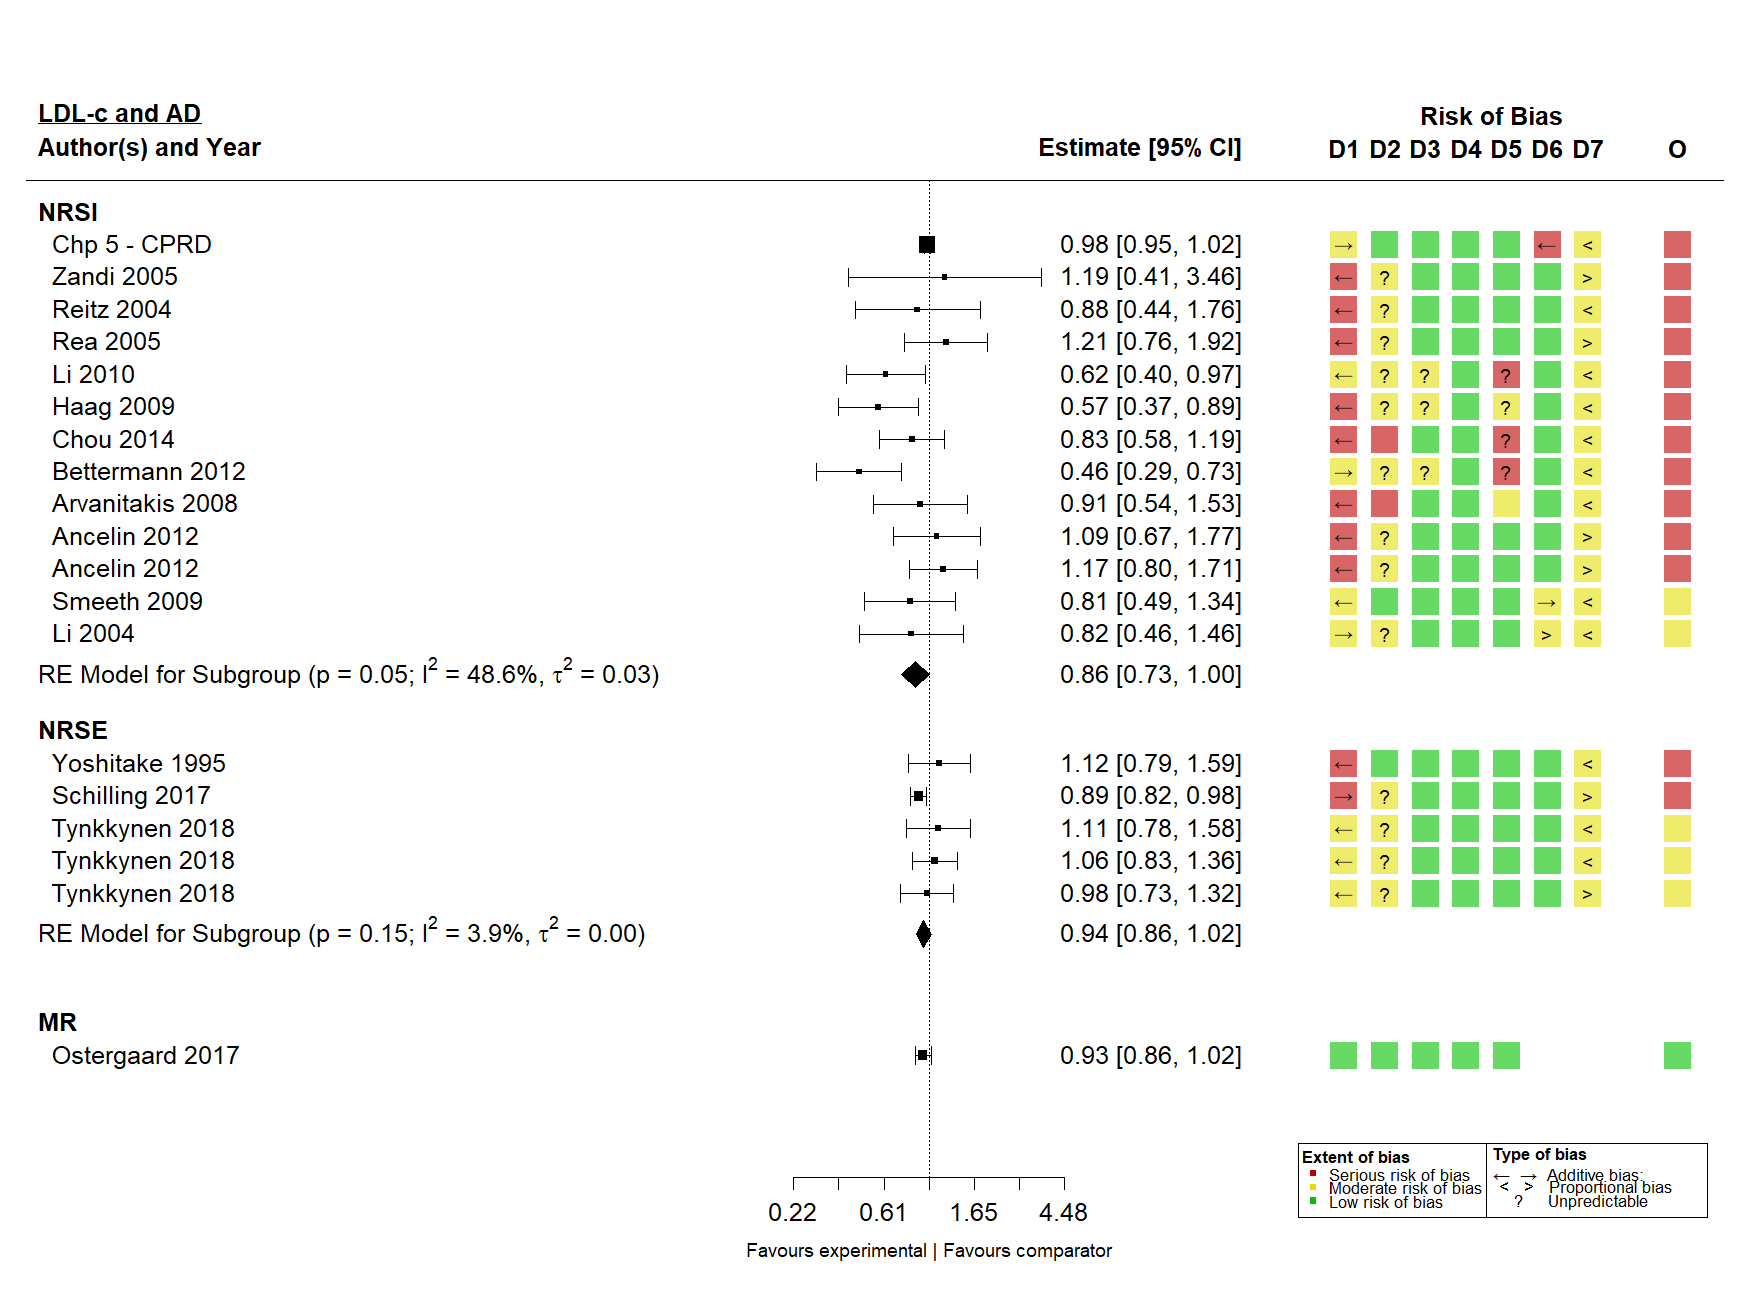
\includegraphics[width=1\linewidth]{figures/tri/midlife_AD} \caption[Bias direction plot, summarising internal biases related to the]{Bias direction plot, summarising the internal biases related to effect of LDL-c on Alzheimer's disease, stratified by study design.}\label{fig:ldlAdBiasDirection}
\end{figure}

~

The results of the unadjusted and the bias-/indirectness-adjusted (under the Scenario 1 of additive biases) are shown in Figure \ref{fig:fpLdlAd}. I observed no substantial change to the overall effect (unadjusted 0.92, 95\%CI: 0.82-1.03; adjusted 1.06, 95\%CI: 0.94-1.19), though adjustment for bias and indirectness substantially reduced the heterogeneity between studies (unadjusted \(\tau^2\) = 0.023922, \(I^2\) = 58.0417167; adjusted \(\tau^2\) = 0, \(I^2\) = 0). However, as can been seen from the right panel in the figure, this reduction in heterogeneity between studies is largely achieved via a reduction in precision.

To explore the different impacts of the two defined scenarios for additive bias, I plotted these:

~





\begin{figure}[H]
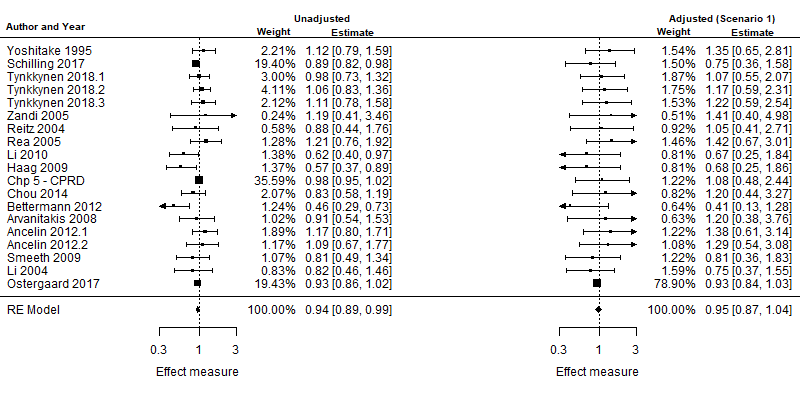
\includegraphics[width=1\linewidth]{figures/tri/fp_paired_midlife_ldl_ad} \caption[Random effects meta-analysis using unadjusted and bias-/indirectness-adjusted results.]{Random effects meta-analysis using unadjusted and bias-/indirectness-adjusted results.}\label{fig:fpLdlAd}
\end{figure}

~

\hypertarget{discussion-4}{%
\section{Discussion}\label{discussion-4}}

\hypertarget{summary-of-findings-3}{%
\subsection{Summary of findings}\label{summary-of-findings-3}}

This chapter has narratively synthesised the existing and new evidence identified and produced by the previous chapters, highlighting the absence of any consistent association between any blood lipid and any dementia outcome in the context of the bias in each approach.

In addition, it has sought to provide a generalised framework for quantitative triangulation, building on existing methods for systematic domain-based risk of bias assessment and bias-/indirectness-adjusted meta-analysis. While a lack of information on the prior distributions of bias and indirectness in non-randomised studies precluded, to illustrate the method, I considered the example causal question of the effect of mid-life LDL-c on Alzheimer's disease risk derived from a previous expert elicitation exercise.

~

\hypertarget{limitations-2}{%
\subsection{Limitations}\label{limitations-2}}

\hypertarget{defining-reasonable-prior-distributions-for-bias-and-indirectness}{%
\subsubsection{Defining reasonable prior distributions for bias and indirectness}\label{defining-reasonable-prior-distributions-for-bias-and-indirectness}}

The key limitation of this quantitative synthesis presented in this chapter is the ambiguity

It is the reason that only one causal question is addressed as a case study, as to base clinical recommendations on a method dependent on non-empirical values would be inappropriate.

Meta-epidemiological studies on the effect of different methodological issues on results exist for randomised controlled trials,\textsuperscript{\protect\hyperlink{ref-amer2021}{320},\protect\hyperlink{ref-page2016}{321}} suggesting that X, Y and Z.

However, there is substantially less , arguably because of the absence of clear
Many meta-epi studies of non-randomised studies assume bias at the study-design level, similar to the early triangulation frame-work, rather than considering the actual biases deemed to be present in a given result. In this scenario, study

Potential future meta-epidemiology studies should begin to create these datasets.

New software for performing risk of bias assessments, being developed by the Bristol Appraisal and Review of Research group has this as a secondary methodological aim.

Much of the attention to date has been on assessing the impact of different sources of bias on effect estimates has focused predominantly on randomised controlled trials.

For example, a study examining the effect of found that only a subset of domains appear to impact the result, and that this effect is modest (10\% change).\textsuperscript{\protect\hyperlink{ref-savovic2018}{322}} However, this work examined RCTs, and these findings may not hold for other non-randomised study designs.

Similar there are several examples of usmeta to define priors for other statistical terms in meta-analysis. For example, previous work has looked at defining prior distributions of heterogeneity across different topic areas using a large collection of meta-analyses from the Cochrane Collaboration.

Elicitation and bias-adjusted not as favoured versus weighting\textsuperscript{\protect\hyperlink{ref-stone2020}{323}} though weighting at the overall risk-of-bias level loses some of the information contained in domain-level based assessments.

~

\hypertarget{low-and-critical-risk-of-bias}{%
\subsubsection{Low and critical risk of bias}\label{low-and-critical-risk-of-bias}}

As illustrated in Table \ref{tab:robLevelsMapping-table}, studies at critical risk of bias were not included in the analysis.

one potential limitation of the - however, the estimation of an appropriate adjustment value for these studies would be substantially more challenging.

In any case, it represented a small number of studies.s

A further issue is the ``Low'' risk of bias domain. In this proof-of-concept analysis, I assumed that domains at ``Low'' risk of bias did not require any adjustment. However, ``Low'' risk of bias is not equivalent to the absence of bias, and potentially should still be adjusted for. In this case, defining the predicted direction of bias would be challenging in the absence of obvious sources of bias (particularly given how challenging it can be when sources of bias are evident within a domain).

~

\hypertarget{strenghts}{%
\subsection{Strenghts}\label{strenghts}}

This approach has a number of advantages. One of the key ones is modifying distributions of each level of bias could be defined \emph{a priori} in contrast to the .

In addition, the generalised framework will allow for future researchers to apply (see Section @ref())

Appreciation that both the risk of bias and indirectness of a result should be assessed is growing. Indeed, some existing risk of bias for the assessment of diagnostic test accurary\textsuperscript{\protect\hyperlink{ref-whiting2011a}{324}} and prediction models\textsuperscript{\protect\hyperlink{ref-moons2019}{325}} consider indirectness (termed applicability in these tools) alongside the assessment of bias. The approach proposed here will capitalise on this, providing users of domain based tools with a further avenue by whih to incorporate the results of their risk-of-bias assessments quantitatively.

Additional if users are interested in only a summary of the evidence rather than assessing results in relation to a target qusetion, then internal biases can be adjusted for on their own.

In previous attempts at bias/indirectness-adjusted meta-analysis, the extent to each was assessed via a elicitation process using a number of experts. This approach is potentially subject to misclassification of the impact of bias on the basis of the results, as there is no way to ensure that results at a similar level of bias for confounding (for example) are being adjusted by the same amount. For example, if experts are influenced by the absolute effect estimate, then a result demonstrating a stronger protective effect may receive greater modification than a study at the same ``risk'' of confounding but with a more modest effect. This is particular true where experts have preconceived ideas about the true effectiveness of the intervention.

In this case, separating the assessment of bias from the assignment of modifying values to each level of bias will limit the potential for. Alternatively, reasonable modifying distributions for each level of bias could be defined \emph{a priori} by the study team, similar to how important confounders and co-interventions are defined in advance when performing ROBINS-I/ROBINS-E assessments.

~

\newpage

\hypertarget{future-research}{%
\subsection{Future research}\label{future-research}}

As the need and appetite for synthesis of different sources of evidence (trials, non-randomised studies, etc.), future iterations of the risk of bias tools should take this into account. Simple steps like harmonising the risk of bias levels across tools would be a good first move towards a more integrate suite of tools. Similarly, software that implements the risk-of-bias tools should both allow for direction of bias question and carefully consider how this data will be exported.

While the limitations inherent to this method are important, and limit the , they reflect a more detailed appreciation of the complexities of risk of bias assessment and triangulation as whole (i.e.~not applying expected directions of effects to an entire category of studies ).

This approach also builds on existing approaches employed previously by ``exploding out'' the results of a systematic review/meta-analysis and considering the effects of bias in each individual result separately. This more granular approach is to be preferred over assigning a bias judgement and direction to the summary effect produced by a meta-analysis, which may mask the different biases applicable to each unique result.

A key example of a useful future study in this domain would be the mining of maximally adjusted vs.~unadjusted estimates from abstracts from primary studies to assess the impact of insufficient confounding by topic. However, these datasets could also be built from systematic reviews of a topic, as they would already be gruped by reserach domain and provided the risk of bias data is shared, provide a ready source of information

In the mean time, the extent of the impact of knowledge of the results could be analysed using existing data. For example, a re-analysis of the data presented in a recent paper where both expert elicitation and structured

~

\hypertarget{triangulation-as-an-extension-of-evidence-synthesis}{%
\subsection{Triangulation as an extension of evidence synthesis}\label{triangulation-as-an-extension-of-evidence-synthesis}}

Triangulation, both qualitative and quantitative, should be considered an extension of evidence synthesis, and so. Triangulation exercises should be based on comprehensive systematic reviews to create. If needed, evidence gaps can be addressed through additional studies, as in the case of this analysis,

Compare and contrast with the nice example presented in the triangulation paper - realities of non-exemplars is that it is very hard to get this right. Also highlight the issue with assigning a direct of bias in many studies

I hope this presents step forward in how researchers think about and visualise triangulation at the result level, rather than simply saying that certain

~

\hypertarget{tri-software}{%
\subsection{Outputs}\label{tri-software}}

There are two key outputs from this project. The first is the \texttt{trinagulate} R package. Personal communication with the authors of the original method resulted in the STATA code to implement the bias-/indirectness-adjusted model. This has since been generalised as part of the \texttt{triangulate} R package to enable other users to apply the approach detailed here. The package allows for preprocessing of domain-based risk-of-bias data to correctly identify the direction of the bias relative to the effect estimate, use of domain-specific prior distributions, calculation of bias/indirectness-adjusted estimates for each result, and synthesis these adjusted results in a standard random-effects meta-analysis. All meta-analyses conducted within the package are implemented using the \texttt{metafor} R package.

Generalised version of code, allowing for different distributions in each domain of bias (which will be handy once we get a better idea of what they should be).

Annotated example dataset for the LDL-c/Alzheimer's disease causal question is the second key output. Available via the \texttt{triangulate} package, this data will give developers of new triangulation methods an example dataset on which to test developments, something which seriously hindered development of this project. This also ties with the idea of open data that has been a consistent theme throughout this thesis.

An additional note is that without the open data sharing of the by-assessor elictation data from, which i sued in this analysis to frame the modifying values assigned to

~

\hypertarget{conclusion-1}{%
\section{Conclusion}\label{conclusion-1}}

Triangulation is a promising developing field, somewhat hamstrung by the limited understanding of the impact of biases at the meta-epidemiological level.

In this chapter, I have presented a new method of visualising both the level and expected direction of bias inherent to each result, and suggested how this could be incorporated with a bias-adjusted meta-analysis approach to work towards a generalised quantitative triangulation framework.

Finally, I've highlighted the limitations of this method, as the correct distributions of modifying values in each risk-of-bias domain should be driven by meta-epidemiological studies which do not yet exist, framing them as opportunities for future research.

This chapter has demonstrated a repurposed framework for quantitative triangulation, exploiting existing methods in evidence synthesis and developments in the assessment of different risks of bias.

Future quantitative triangulation should move beyond the concept of comparing results at the approach level, and instead focus on the inherent threats to the internal validity and directness of each specific result relevant to the causal question. While this makes the process both more labour intensive and complex,

It also introduce a new way to visualise the biases at work in a particular result, rather than making assumptions about the type and directions of bias at the study design level as suggested by previous work on this topic.

Finally, it highlighted the limitations of current methods for triangulation in the absence of informative priors for the impact of biases across the

The implications of th synthesised work of this thesis presened in this chapter to clinical practice, public health and future research is considered in the following chapter.

\newpage

\hypertarget{references-5}{%
\section{References}\label{references-5}}

--- Hold --- Hold

\hypertarget{discussion-heading}{%
\chapter{Discussion}\label{discussion-heading}}

\minitoc 

~

\hypertarget{lay-summary-6}{%
\section{Lay summary}\label{lay-summary-6}}

This chapter

\hypertarget{chapter-overview}{%
\section{Chapter overview}\label{chapter-overview}}

In this chapter I will summarise the principal findings from my thesis,

assess the unique contributions of this thesis to the field of research,

discuss the implications for both clinical and public health policy,

describe the overall strengths and limitations of this thesis as a whole,

suggest avenues for impactful future research based on my findings and experiences.

~

\hypertarget{summary-of-principal-findings}{%
\section{Summary of principal findings}\label{summary-of-principal-findings}}

Given the detailed discussion

~

\hypertarget{new-evidence}{%
\section{New evidence}\label{new-evidence}}

Found slight raised risk of dementia in CPRD patients () with higher LDL-c measured at midlife, driven by the finding for Alzheimer's disease.\textsuperscript{\protect\hyperlink{ref-iwagami2021}{326}} Not inconsistent with the findings presented in this thesis

\hypertarget{lessons-learned}{%
\section{Lessons learned}\label{lessons-learned}}

There are

~

\hypertarget{overall-strengths-and-limitations}{%
\section{Overall strengths and limitations}\label{overall-strengths-and-limitations}}

This thesis has used multiple sources of evidence to examine the relationship between blood lipids levels and cholesterol risk.

It has highlighted the importance of including preprints in systematic review, and provided a tool to enable researchers to easily do so.

It has analysed two previously unanalysed datasets, adding useful information to the evidence base.

However, the thesis as a whole is subject to some strong limitations.

There are several strengths and limitations to the work presented in this thesis. One particularly strength is the lengths gone to find all available published and unpublished evidence around the question, and to integrate this evidence in a coherent framework, taking into account the limitations of ach source and how these limitations may be used to provide

Need for large simple trials for common disease where small treatment effect can have large effect -\textsuperscript{\protect\hyperlink{ref-yusuf1984}{327}}

This thesis is limited by the low response rate to data access requests, and the

The lack of large, precise studies made comparison across different types of evidence difficult, while the low number of eligible studies for a

~

\hypertarget{implications-of-this-research}{%
\section{Implications of this research}\label{implications-of-this-research}}

\hypertarget{clinical-practice}{%
\subsection{Clinical practice}\label{clinical-practice}}

Across multiple sources of evidence, there was no consistent effect of blood lipids, or . Some

The clinical recommendations that can be drawn from the work in this thesis are limited, due to the low strength of evidence related to the

There was very we. Conversely however, there was an absence of evidence for a harmful effect of statins on. Given the reality that given the choice, given the conflicting evidence

Patients must live to a sufficient age to be at risk of dementia outcomes, which is substantially less like if high lipid levels in mid-life.

The role of lipid-lowering

As with many many studies of dementia outcomes, a key limiting factor of any analysis is the absence of a detailed pathological mechanism for Alzheimer's disease. It could well be that statins do have a true effect independently of lipid levels, though based on the certainty of evidence in NRSI, this is unlikely.

However, based on the available evidence

For other dementia outcomes,

~

\hypertarget{public-health}{%
\subsection{Public health}\label{public-health}}

~

\hypertarget{reproducible-research}{%
\section{Reproducible research}\label{reproducible-research}}

Reproducible and science has been a key theme running through this thesis, as reflected by the development of an open source tool to help search medRxiv and bioRxiv preprint metadata. In line with this, an open source copy of the code used to produce this thesis is available on GitHub, as is the code used to perform the analysis contained within it.

Containerisation was used to ensure that the code is reproducible, in line iwht best practices

Commentary on the fact that the best you can do is replicate vs reproducible (due the closed nature of the data).

One is the ability to recreate the results given the same data and code, the other is the ability to recreate the results given the same code but a different dataset. IN theory it is possible to gain access the dataset given the information presented in Chapter @(ref:cprd-analysis-heading). However, access is dependency on an ISAC application to the managing body of the CPRD.

~

\hypertarget{disc-PPI}{%
\section{Public involvement and engagement}\label{disc-PPI}}

Involving and engaging the public and patients has been a central theme to this thesis.
Public engagement activities included

Public involvement also steered the creation of the topic

~

\hypertarget{future-work}{%
\section{Future work}\label{future-work}}

Several avenues for future research, buiding on the work presented here,

\hypertarget{section}{%
\subsection{}\label{section}}

\hypertarget{inclusion-of-preprints-1}{%
\subsection{Inclusion of preprints}\label{inclusion-of-preprints-1}}

Normalisation of inclusion of preprints in systematic reviews. Wider assessment of the evidence base that exists solely as preprinted literature ()

Studying of factors which influence eventual publication would also help to identify the extent and strength of publication bias by providing a

Preprints also represent a key oppportunity to assess the impact of peer review on qualitivative changes within

~

\hypertarget{evidence-on-vascular-dementia}{%
\subsection{Evidence on vascular dementia}\label{evidence-on-vascular-dementia}}

As discussed, there is an absence of evidence on vascular dementia across the evidence base, potentially driven y

large-scale GWAS of vascular dementia should be performed, to identify associated loci that future Mendelian randomisation studies can make use of. While this is methodologically challenging, given the difficult in diagnosing ``pure'' vascular dementia, it would be a worthwhile endeavour, and would allow for the assessment of many genetically driven risk factors beyond those considered in this thesis.

~

\hypertarget{reviewing-of-mendelian-randomisation-studies}{%
\subsection{Reviewing of Mendelian randomisation studies}\label{reviewing-of-mendelian-randomisation-studies}}

As a field, and as noted in Chapter \ref{sys-rev-heading-results}, the evidence synthesis theory and methods have not been sufficient developed for Mendelian randomisation studies. Future work should aim to validate search strategies for this study design, paying particular attention to the range of terms used to define it (e.g.~genetic instrumental variable analysis.)

Work is ongoing in this field, and new methodological work such as the release of teh MR-STROBE guidelines will aid in the future assessing by helping to improve the reporting of Mendelian randomisation studies.

Problems with reporting of MR studies will hopefully

~

\hypertarget{empirical-estimates-of-bias}{%
\subsection{Empirical estimates of bias}\label{empirical-estimates-of-bias}}

Finally, substantial future work should be directed towards the conduct of meta-epidemiological studies to assess the impact of different bias in non-observational studies. While frameworks such as the one employed in Chapter \ref{tri-heading} exist to allow for the production of bias-adjusted and triangulated estimates.

~

\hypertarget{imporved-analytical-designs}{%
\subsection{Imporved analytical designs}\label{imporved-analytical-designs}}

Use of the real-world evidence approach needs to be traded off against the important limitations that t

Talk about the problems with real world evidence, and highlight that even when using these techniques, you still don't get the correct answers.

Tie in with GDS comments on off-targets effect.

~

\hypertarget{overall-conclusions}{%
\section{Overall conclusions}\label{overall-conclusions}}

This thesis has made unique and novel contributions to the

Illustrating that commonly employed approaches to address

Definition of covariates adjusted for in the full-adjusted model. The codelists used to define the majority of these covariates were originally created for use in a previously published analysis.\textsuperscript{\protect\hyperlink{ref-walker2020}{272}} while others were built on or adapted from previous published work,\textsuperscript{\protect\hyperlink{ref-khan2010}{273}--\protect\hyperlink{ref-wright2017}{275}}. Definition of covariates adjusted for in the full-adjusted model. The codelists used to define the majority of these covariates were originally created for use in a previously published analysis.\textsuperscript{\protect\hyperlink{ref-walker2020}{272}} while others were built on or adapted from previous published work.\textsuperscript{\protect\hyperlink{ref-khan2010}{273}--\protect\hyperlink{ref-wright2017}{275}}

Covariates adjusted for. Covariates adjusted for.

Charlson index implemented using Read code lists.\textsuperscript{\protect\hyperlink{ref-khan2010}{273}} Code lists based on those by Taylor et al.\textsuperscript{\protect\hyperlink{ref-taylor2016}{274}} Charlson index implemented using Read code lists.\textsuperscript{\protect\hyperlink{ref-khan2010}{273}} Code lists based on those by Taylor et al.\textsuperscript{\protect\hyperlink{ref-taylor2016}{274}}

Most recent of recorded value (current, former or never) or Read code indicating a recorded value. Code lists based on those by Wright et al.\textsuperscript{\protect\hyperlink{ref-wright2017}{275}} Most recent of recorded value (current, former or never) or Read code indicating a recorded value. Code lists based on those by Wright et al.\textsuperscript{\protect\hyperlink{ref-wright2017}{275}}

Charlson index implemented using Read code lists.\textsuperscript{\protect\hyperlink{ref-khan2010}{273}} Code lists based on those by Taylor et al.\textsuperscript{\protect\hyperlink{ref-taylor2016}{274}}

\begin{table}[H]

\caption[Covariates adjusted for.]{\label{tab:covariateDef-table}Definition of covariates adjusted for in the full-adjusted model. The codelists used to define the majority of these covariates were originally created for use in a previously published analysis.\textsuperscript{\protect\hyperlink{ref-walker2020}{272}} while others were built on or adapted from previous published work,\textsuperscript{\protect\hyperlink{ref-khan2010}{273}--\protect\hyperlink{ref-wright2017}{275}}.}
\centering
\fontsize{9}{11}\selectfont
\begin{tabular}[t]{>{\raggedright\arraybackslash}p{15em}>{\centering\arraybackslash}p{25em}}
\toprule
\textbf{Covariate } & \textbf{How was the covariate defined?}\\
\midrule
Previous history of coronary arterial disease & Presence of one or more relevant Read codes on record.\\
\midrule
Previous history of coronary bypass surgery & Presence of one or more relevant Read codes on record.\\
\midrule
Previous history of cerebrovascular disease (including stroke) & Presence of one or more relevant Read codes on record.\\
\midrule
Chronic illness, including cancer and arthritis & Charlson index implemented using Read code lists.\textsuperscript{\protect\hyperlink{ref-khan2010}{273}} Code lists based on those by Taylor et al.\textsuperscript{\protect\hyperlink{ref-taylor2016}{274}}\\
\midrule
Socioeconomic position & 2010 English Index of Multiple Deprivation (IMD) at the twentile level, where 1 represents the least deprived and 20 the most deprived.\\
\midrule
\addlinespace
Consultation rate & Calculated by dividing the total number of clinic visits by the length of the patient record prior to the index date to give an average annual rate.\\
\midrule
Alcohol status & Recorded value (current, former or never).\\
\midrule
Smoking status & Most recent of recorded value (current, former or never) or Read code indicating a recorded value. Code lists based on those by Wright et al.\textsuperscript{\protect\hyperlink{ref-wright2017}{275}}\\
\midrule
Body Mass Index & Recorded value if available, or a calculated value using the last recorded height and weight measurements. Measurements taken before the age of 25 were excluded to ensure adult measurements were used.\\
\midrule
Peripheral arterial disease & Presence of one or more relevant Read codes on record.\\
\midrule
\addlinespace
Hypertension & Presence of one or more relevant Read codes on record.\\
\midrule
Baseline total cholesterol & Continuous value recorded as test result ("enttype==163 \& test\_data1==3")\\
\midrule
Baseline LDL cholesterol & Continuous value recorded as test result ("enttype==177 \& test\_data1==3")\\
\midrule
Chronic kidney disease & Presence of one or more relevant Read codes on record.\\
\midrule
Type 1 Diabetes & Presence of one or more relevant Read codes on record.\\
\midrule
\addlinespace
Type 2 Diabetes & Presence of one or more relevant Read codes on record.\\
\bottomrule
\end{tabular}
\end{table}

\begin{savequote}
Lasciate ogne speranza, voi ch'intrate. . .
\end{savequote}

\hypertarget{bibliography}{%
\chapter{Bibliography}\label{bibliography}}

\hypertarget{refs}{}
\begin{CSLReferences}{0}{0}
\leavevmode\hypertarget{ref-cerejeira2012}{}%
\CSLLeftMargin{1. }
\CSLRightInline{Cerejeira, J., Lagarto, L. \& Mukaetova-Ladinska, E. B. Behavioral and {Psychological Symptoms} of {Dementia}. \emph{Frontiers in Neurology} \textbf{3}, (2012).}

\leavevmode\hypertarget{ref-kumar2013}{}%
\CSLLeftMargin{2. }
\CSLRightInline{Kumar, C. S. \& Kuriakose, J. R. End-of-life care issues in advanced dementia. \emph{Mental Health in Family Medicine} \textbf{10}, 129--132 (2013).}

\leavevmode\hypertarget{ref-burns2009}{}%
\CSLLeftMargin{3. }
\CSLRightInline{Burns, A. \& Iliffe, S. Dementia. \emph{BMJ} \textbf{338}, b75 (2009).}

\leavevmode\hypertarget{ref-robinson2015}{}%
\CSLLeftMargin{4. }
\CSLRightInline{Robinson, L., Tang, E. \& Taylor, J.-P. Dementia: Timely diagnosis and early intervention. \emph{BMJ} \textbf{350}, h3029 (2015).}

\leavevmode\hypertarget{ref-iadecola2013}{}%
\CSLLeftMargin{5. }
\CSLRightInline{Iadecola, C. The pathobiology of vascular dementia. \emph{Neuron} \textbf{80}, (2013).}

\leavevmode\hypertarget{ref-venkat2015}{}%
\CSLLeftMargin{6. }
\CSLRightInline{Venkat, P., Chopp, M. \& Chen, J. Models and {Mechanisms} of {Vascular Dementia}. \emph{Experimental neurology} \textbf{272}, 97--108 (2015).}

\leavevmode\hypertarget{ref-custodio2017}{}%
\CSLLeftMargin{7. }
\CSLRightInline{Custodio, N. \emph{et al.} Mixed dementia: A review of the evidence. \emph{Dementia \& Neuropsychologia} \textbf{11}, 364--370 (2017).}

\leavevmode\hypertarget{ref-sheehan2012}{}%
\CSLLeftMargin{8. }
\CSLRightInline{Sheehan, B. Assessment scales in dementia. \emph{Therapeutic Advances in Neurological Disorders} \textbf{5}, 349--358 (2012).}

\leavevmode\hypertarget{ref-dubois2007}{}%
\CSLLeftMargin{9. }
\CSLRightInline{Dubois, B. \emph{et al.} Research criteria for the diagnosis of {Alzheimer}'s disease: Revising the {NINCDS}{{ADRDA}} criteria. \emph{The Lancet Neurology} \textbf{6}, 734--746 (2007).}

\leavevmode\hypertarget{ref-prince2016}{}%
\CSLLeftMargin{10. }
\CSLRightInline{Prince, M. \emph{et al.} Recent global trends in the prevalence and incidence of dementia, and survival with dementia. \emph{Alzheimer's Research \& Therapy} \textbf{8}, 23 (2016).}

\leavevmode\hypertarget{ref-flier2005}{}%
\CSLLeftMargin{11. }
\CSLRightInline{Flier, W. M. van der \& Scheltens, P. Epidemiology and risk factors of dementia. \emph{Journal of Neurology, Neurosurgery \& Psychiatry} \textbf{76}, v2--v7 (2005).}

\leavevmode\hypertarget{ref-baker2019}{}%
\CSLLeftMargin{12. }
\CSLRightInline{Baker, C., Jarrett, T. \& Powell, T. \emph{Dementia: Policy, services and statistics overview}. (2019).}

\leavevmode\hypertarget{ref-wittenberg2019}{}%
\CSLLeftMargin{13. }
\CSLRightInline{Wittenberg, R. \emph{et al.} The costs of dementia in {England}. \emph{International Journal of Geriatric Psychiatry} \textbf{34}, 1095--1103 (2019).}

\leavevmode\hypertarget{ref-cummings2020}{}%
\CSLLeftMargin{14. }
\CSLRightInline{Cummings, J., Lee, G., Ritter, A., Sabbagh, M. \& Zhong, K. Alzheimer's disease drug development pipeline: 2020. \emph{Alzheimer's \& Dementia: Translational Research \& Clinical Interventions} \textbf{6}, e12050 (2020).}

\leavevmode\hypertarget{ref-hampel2018}{}%
\CSLLeftMargin{15. }
\CSLRightInline{Hampel, H. \emph{et al.} The cholinergic system in the pathophysiology and treatment of {Alzheimer}'s disease. \emph{Brain} \textbf{141}, 1917--1933 (2018).}

\leavevmode\hypertarget{ref-pariente2008}{}%
\CSLLeftMargin{16. }
\CSLRightInline{Pariente, A. \emph{et al.} Prevalence of cholinesterase inhibitors in subjects with dementia in {Europe}. \emph{Pharmacoepidemiology and Drug Safety} \textbf{17}, 655--660 (2008).}

\leavevmode\hypertarget{ref-marucci2020}{}%
\CSLLeftMargin{17. }
\CSLRightInline{Marucci, G. \emph{et al.} Efficacy of acetylcholinesterase inhibitors in {Alzheimer}'s disease. \emph{Neuropharmacology} 108352 (2020). doi:\href{https://doi.org/10.1016/j.neuropharm.2020.108352}{10.1016/j.neuropharm.2020.108352}}

\leavevmode\hypertarget{ref-francis2010}{}%
\CSLLeftMargin{18. }
\CSLRightInline{Francis, P. T., Ramírez, M. J. \& Lai, M. K. Neurochemical basis for symptomatic treatment of {Alzheimer}'s disease. \emph{Neuropharmacology} \textbf{59}, 221--229 (2010).}

\leavevmode\hypertarget{ref-feingold2000}{}%
\CSLLeftMargin{19. }
\CSLRightInline{Feingold, K. R. Introduction to {Lipids} and {Lipoproteins}. in \emph{Endotext} (eds. Feingold, K. R. et al.) ({MDText.com, Inc.}, 2000).}

\leavevmode\hypertarget{ref-peters2019}{}%
\CSLLeftMargin{20. }
\CSLRightInline{Peters, R. \emph{et al.} Combining modifiable risk factors and risk of dementia: A systematic review and meta-analysis. \emph{BMJ Open} \textbf{9}, e022846 (2019).}

\leavevmode\hypertarget{ref-anstey2019}{}%
\CSLLeftMargin{21. }
\CSLRightInline{Anstey, K. J., Ee, N., Eramudugolla, R., Jagger, C. \& Peters, R. A {Systematic Review} of {Meta}-{Analyses} that {Evaluate Risk Factors} for {Dementia} to {Evaluate} the {Quantity}, {Quality}, and {Global Representativeness} of {Evidence}. \emph{Journal of Alzheimer's Disease} \textbf{70}, S165--S186 (2019).}

\leavevmode\hypertarget{ref-norton2014potential}{}%
\CSLLeftMargin{22. }
\CSLRightInline{Norton, S., Matthews, F. E., Barnes, D. E., Yaffe, K. \& Brayne, C. Potential for primary prevention of {Alzheimer}'s disease: An analysis of population-based data. \emph{The Lancet Neurology} \textbf{13}, 788--794 (2014).}

\leavevmode\hypertarget{ref-laufs2020}{}%
\CSLLeftMargin{23. }
\CSLRightInline{Laufs, U., Parhofer, K. G., Ginsberg, H. N. \& Hegele, R. A. Clinical review on triglycerides. \emph{European Heart Journal} \textbf{41}, 99--109c (2020).}

\leavevmode\hypertarget{ref-zampelas2019}{}%
\CSLLeftMargin{24. }
\CSLRightInline{Zampelas, A. \& Magriplis, E. New {Insights} into {Cholesterol Functions}: A {Friend} or an {Enemy}? \emph{Nutrients} \textbf{11}, (2019).}

\leavevmode\hypertarget{ref-friedewald1972}{}%
\CSLLeftMargin{25. }
\CSLRightInline{Friedewald, W. T., Levy, R. I. \& Fredrickson, D. S. Estimation of the {Concentration} of {Low}-{Density Lipoprotein Cholesterol} in {Plasma}, {Without Use} of the {Preparative Ultracentrifuge}. \emph{Clinical Chemistry} \textbf{18}, 499--502 (1972).}

\leavevmode\hypertarget{ref-national2002third}{}%
\CSLLeftMargin{26. }
\CSLRightInline{Detection, N. C. E. P. (US). E. P. on. \emph{Third report of the {National Cholesterol Education Program} ({NCEP}) {Expert Panel} on detection, evaluation, and treatment of high blood cholesterol in adults ({Adult Treatment Panel III})}. ({The Program}, 2002).}

\leavevmode\hypertarget{ref-nelson2013}{}%
\CSLLeftMargin{27. }
\CSLRightInline{Nelson, R. H. Hyperlipidemia as a {Risk Factor} for {Cardiovascular Disease}. \emph{Primary care} \textbf{40}, 195--211 (2013).}

\leavevmode\hypertarget{ref-libby2019}{}%
\CSLLeftMargin{28. }
\CSLRightInline{Libby, P. \emph{et al.} Atherosclerosis. \emph{Nature Reviews Disease Primers} \textbf{5}, 1--18 (2019).}

\leavevmode\hypertarget{ref-collins2016}{}%
\CSLLeftMargin{29. }
\CSLRightInline{Collins, R. \emph{et al.} Interpretation of the evidence for the efficacy and safety of statin therapy. \emph{The Lancet} \textbf{388}, 2532--2561 (2016).}

\leavevmode\hypertarget{ref-collins2016a}{}%
\CSLLeftMargin{30. }
\CSLRightInline{Collins, R. \emph{et al.} Interpretation of the evidence for the efficacy and safety of statin therapy. \emph{The Lancet} \textbf{388}, 2532--2561 (2016).}

\leavevmode\hypertarget{ref-law2003}{}%
\CSLLeftMargin{31. }
\CSLRightInline{Law, M. R., Wald, N. J. \& Rudnicka, A. R. Quantifying effect of statins on low density lipoprotein cholesterol, ischaemic heart disease, and stroke: Systematic review and meta-analysis. \emph{BMJ} \textbf{326}, 1423 (2003).}

\leavevmode\hypertarget{ref-schachter2005}{}%
\CSLLeftMargin{32. }
\CSLRightInline{Schachter, M. Chemical, pharmacokinetic and pharmacodynamic properties of statins: An update. \emph{Fundamental \& Clinical Pharmacology} \textbf{19}, 117--125 (2005).}

\leavevmode\hypertarget{ref-sierra2011}{}%
\CSLLeftMargin{33. }
\CSLRightInline{Sierra, S. \emph{et al.} Statins as neuroprotectants: A comparative in vitro study of lipophilicity, blood-brain-barrier penetration, lowering of brain cholesterol, and decrease of neuron cell death. \emph{Journal of Alzheimer's disease: JAD} \textbf{23}, 307--318 (2011).}

\leavevmode\hypertarget{ref-kosoglou2005}{}%
\CSLLeftMargin{34. }
\CSLRightInline{Kosoglou, T. \emph{et al.} Ezetimibe: A review of its metabolism, pharmacokinetics and drug interactions. \emph{Clinical Pharmacokinetics} \textbf{44}, 467--494 (2005).}

\leavevmode\hypertarget{ref-genest2006}{}%
\CSLLeftMargin{35. }
\CSLRightInline{Genest, J. Combination of statin and ezetimibe for the treatment of dyslipidemias and the prevention of coronary artery disease. \emph{The Canadian Journal of Cardiology} \textbf{22}, 863--867 (2006).}

\leavevmode\hypertarget{ref-chaudhary2017}{}%
\CSLLeftMargin{36. }
\CSLRightInline{Chaudhary, R., Garg, J., Shah, N. \& Sumner, A. {PCSK9} inhibitors: A new era of lipid lowering therapy. \emph{World Journal of Cardiology} \textbf{9}, 76--91 (2017).}

\leavevmode\hypertarget{ref-mckenney2004new}{}%
\CSLLeftMargin{37. }
\CSLRightInline{McKenney, J. New perspectives on the use of niacin in the treatment of lipid disorders. \emph{Archives of internal medicine} \textbf{164}, 697--705 (2004).}

\leavevmode\hypertarget{ref-skulas-rayannc.2019}{}%
\CSLLeftMargin{38. }
\CSLRightInline{Skulas-Ray Ann C. \emph{et al.} Omega-3 {Fatty Acids} for the {Management} of {Hypertriglyceridemia}: A {Science Advisory From} the {American Heart Association}. \emph{Circulation} \textbf{140}, e673--e691 (2019).}

\leavevmode\hypertarget{ref-burns2003}{}%
\CSLLeftMargin{39. }
\CSLRightInline{Burns, M. P. \emph{et al.} Co-localization of cholesterol, apolipoprotein {E} and fibrillar {A\(\beta\)} in amyloid plaques. \emph{Molecular Brain Research} \textbf{110}, 119--125 (2003).}

\leavevmode\hypertarget{ref-mizuno1999}{}%
\CSLLeftMargin{40. }
\CSLRightInline{Mizuno, T. \emph{et al.} Cholesterol-dependent {Generation} of a {Seeding Amyloid} {\(\beta\)}-{Protein} in {Cell Culture} *. \emph{Journal of Biological Chemistry} \textbf{274}, 15110--15114 (1999).}

\leavevmode\hypertarget{ref-beecham2014}{}%
\CSLLeftMargin{41. }
\CSLRightInline{Beecham, G. W. \emph{et al.} Genome-{Wide Association Meta}-analysis of {Neuropathologic Features} of {Alzheimer}'s {Disease} and {Related Dementias}. \emph{PLoS Genetics} \textbf{10}, (2014).}

\leavevmode\hypertarget{ref-harold2009}{}%
\CSLLeftMargin{42. }
\CSLRightInline{Harold, D. \emph{et al.} Genome-wide association study identifies variants at {CLU} and {PICALM} associated with {Alzheimer}'s disease, and shows evidence for additional susceptibility genes. \emph{Nature genetics} \textbf{41}, 1088--1093 (2009).}

\leavevmode\hypertarget{ref-meng2007}{}%
\CSLLeftMargin{43. }
\CSLRightInline{Meng, Y. \emph{et al.} Association between {SORL1} and {Alzheimer} disease in a genome-wide study. \emph{Neuroreport} \textbf{18}, 1761--1764 (2007).}

\leavevmode\hypertarget{ref-kivipelto2002}{}%
\CSLLeftMargin{44. }
\CSLRightInline{Kivipelto, M. \emph{et al.} Apolipoprotein {E} {\(E\)}4 {Allele}, {Elevated Midlife Total Cholesterol Level}, and {High Midlife Systolic Blood Pressure Are Independent Risk Factors} for {Late}-{Life Alzheimer Disease}. \emph{Annals of Internal Medicine} \textbf{137}, 149--155 (2002).}

\leavevmode\hypertarget{ref-kivipelto2005}{}%
\CSLLeftMargin{45. }
\CSLRightInline{Kivipelto, M. \emph{et al.} Obesity and vascular risk factors at midlife and the risk of dementia and {Alzheimer} disease. \emph{Archives of Neurology} \textbf{62}, 1556--1560 (2005).}

\leavevmode\hypertarget{ref-schilling2017}{}%
\CSLLeftMargin{46. }
\CSLRightInline{Schilling, S. \emph{et al.} Differential associations of plasma lipids with incident dementia and dementia subtypes in the {3C Study}: A longitudinal, population-based prospective cohort study. \emph{PLoS medicine} \textbf{14}, e1002265 (2017).}

\leavevmode\hypertarget{ref-solomon2009}{}%
\CSLLeftMargin{47. }
\CSLRightInline{Solomon, A., Kivipelto, M., Wolozin, B., Zhou, J. \& Whitmer, R. A. Midlife {Serum Cholesterol} and {Increased Risk} of {Alzheimer}'s and {Vascular Dementia Three Decades Later}. \emph{Dementia and Geriatric Cognitive Disorders} \textbf{28}, 75--80 (2009).}

\leavevmode\hypertarget{ref-whitmer2005}{}%
\CSLLeftMargin{48. }
\CSLRightInline{Whitmer, R. A., Sidney, S., Selby, J., Johnston, S. C. \& Yaffe, K. Midlife cardiovascular risk factors and risk of dementia in late life. \emph{Neurology} \textbf{64}, 277--281 (2005).}

\leavevmode\hypertarget{ref-li2005a}{}%
\CSLLeftMargin{49. }
\CSLRightInline{Li, G. \emph{et al.} Serum cholesterol and risk of {Alzheimer} disease: A community-based cohort study. \emph{Neurology} \textbf{65}, 1045--1050 (2005).}

\leavevmode\hypertarget{ref-mainous2005}{}%
\CSLLeftMargin{50. }
\CSLRightInline{Mainous, A. G., Eschenbach, S. L., Wells, B. J., Everett, C. J. \& Gill, J. M. Cholesterol, transferrin saturation, and the development of dementia and {Alzheimer}'s disease: Results from an 18-year population-based cohort. \emph{Family Medicine} \textbf{37}, 36--42 (2005).}

\leavevmode\hypertarget{ref-mielke2010}{}%
\CSLLeftMargin{51. }
\CSLRightInline{Mielke, M. M. \emph{et al.} The 32-year relationship between cholesterol and dementia from midlife to late life. \emph{Neurology} \textbf{75}, 1888--1895 (2010).}

\leavevmode\hypertarget{ref-tan2003a}{}%
\CSLLeftMargin{52. }
\CSLRightInline{Tan, Z. S. \emph{et al.} Plasma total cholesterol level as a risk factor for {Alzheimer} disease - {The Framingham} study. \emph{Archives of Internal Medicine} \textbf{163}, 1053--+ (2003).}

\leavevmode\hypertarget{ref-mielke2005}{}%
\CSLLeftMargin{53. }
\CSLRightInline{Mielke, M. M. \emph{et al.} High total cholesterol levels in late life associated with a reduced risk of dementia. \emph{Neurology} \textbf{64}, 1689--1695 (2005).}

\leavevmode\hypertarget{ref-reitz2004a}{}%
\CSLLeftMargin{54. }
\CSLRightInline{Reitz, C., Tang, M. X., Luchsinger, J. \& Mayeux, R. Relation of plasma lipids to {Alzheimer} disease and vascular dementia. \emph{Archives of Neurology} \textbf{61}, 705--714 (2004).}

\leavevmode\hypertarget{ref-moroney1999}{}%
\CSLLeftMargin{55. }
\CSLRightInline{Moroney, J. T. Low-{Density Lipoprotein Cholesterol} and the {Risk} of {Dementia With Stroke}. \emph{JAMA} \textbf{282}, 254 (1999).}

\leavevmode\hypertarget{ref-anstey2015}{}%
\CSLLeftMargin{56. }
\CSLRightInline{Anstey, K. J., Ashby-Mitchell, K. \& Peters, R. Updating the {Evidence} on the {Association} between {Serum Cholesterol} and {Risk} of~{Late}-{Life Dementia}: Review and~{Meta}-{Analysis}. \emph{Journal of Alzheimer's Disease} \textbf{56}, 215--228 (2015).}

\leavevmode\hypertarget{ref-chu2018}{}%
\CSLLeftMargin{57. }
\CSLRightInline{Chu, C.-S. \emph{et al.} Use of statins and the risk of dementia and mild cognitive impairment: A systematic review and meta-analysis. \emph{Scientific Reports} \textbf{8}, 5804 (2018).}

\leavevmode\hypertarget{ref-ritchie2015}{}%
\CSLLeftMargin{58. }
\CSLRightInline{Ritchie, C. W., Terrera, G. M. \& Quinn, T. J. Dementia trials and dementia tribulations: Methodological and analytical challenges in dementia research. \emph{Alzheimer's Research \& Therapy} \textbf{7}, 31 (2015).}

\leavevmode\hypertarget{ref-trompet2010}{}%
\CSLLeftMargin{59. }
\CSLRightInline{Trompet, S. \emph{et al.} Pravastatin and cognitive function in the elderly. {Results} of the {PROSPER} study. \emph{Journal of Neurology} \textbf{257}, 85--90 (2010).}

\leavevmode\hypertarget{ref-daveysmith2014}{}%
\CSLLeftMargin{60. }
\CSLRightInline{Davey Smith, G. \& Hemani, G. Mendelian randomization: Genetic anchors for causal inference in epidemiological studies. \emph{Human Molecular Genetics} \textbf{23}, R89--R98 (2014).}

\leavevmode\hypertarget{ref-greenland2000}{}%
\CSLLeftMargin{61. }
\CSLRightInline{Greenland, S. An introduction to instrumental variables for epidemiologists. \emph{International Journal of Epidemiology} \textbf{29}, 722--729 (2000).}

\leavevmode\hypertarget{ref-davies2018}{}%
\CSLLeftMargin{62. }
\CSLRightInline{Davies, N. M., Holmes, M. V. \& Smith, G. D. Reading {Mendelian} randomisation studies: A guide, glossary, and checklist for clinicians. \emph{BMJ} \textbf{362}, k601 (2018).}

\leavevmode\hypertarget{ref-larsson2017c}{}%
\CSLLeftMargin{63. }
\CSLRightInline{Larsson, S. C. \emph{et al.} Modifiable pathways in {Alzheimer}'s disease: Mendelian randomisation analysis. \emph{BMJ} \textbf{359}, j5375 (2017).}

\leavevmode\hypertarget{ref-ostergaard2015}{}%
\CSLLeftMargin{64. }
\CSLRightInline{Østergaard, S. D. \emph{et al.} Associations between {Potentially Modifiable Risk Factors} and {Alzheimer Disease}: A {Mendelian Randomization Study}. \emph{PLOS Medicine} \textbf{12}, e1001841 (2015).}

\leavevmode\hypertarget{ref-kim2009}{}%
\CSLLeftMargin{65. }
\CSLRightInline{Kim, J., Basak, J. M. \& Holtzman, D. M. The {Role} of {Apolipoprotein E} in {Alzheimer}'s {Disease}. \emph{Neuron} \textbf{63}, 287--303 (2009).}

\leavevmode\hypertarget{ref-benn2017}{}%
\CSLLeftMargin{66. }
\CSLRightInline{Benn, M., Nordestgaard, B. G., Frikke-Schmidt, R. \& Tybjærg-Hansen, A. Low {LDL} cholesterol, {PCSK9} and {HMGCR} genetic variation, and risk of {Alzheimer}'s disease and {Parkinson}'s disease: Mendelian randomisation study. \emph{BMJ} \textbf{357}, j1648 (2017).}

\leavevmode\hypertarget{ref-donnelly2018a}{}%
\CSLLeftMargin{67. }
\CSLRightInline{Donnelly, C. A. \emph{et al.} Four principles to make evidence synthesis more useful for policy. \emph{Nature} \textbf{558}, 361--364 (2018).}

\leavevmode\hypertarget{ref-chandler2019chapter}{}%
\CSLLeftMargin{68. }
\CSLRightInline{Chandler, J., Higgins, J., Deeks, J., Davenport, C. \& Clarke, M. J. Chapter 1: introduction. in \emph{Cochrane {Handbook} for {Systematic Reviews} of {Interventions} version 6.2 (updated {February} 2021)} \textbf{5}, ({Cochrane}, 2020).}

\leavevmode\hypertarget{ref-conn2003}{}%
\CSLLeftMargin{69. }
\CSLRightInline{Conn, V. S., Valentine, J. C., Cooper, H. M. \& Rantz, M. J. Grey literature in meta-analyses. \emph{Nursing Research} \textbf{52}, 256--261 (2003 Jul-Aug).}

\leavevmode\hypertarget{ref-mcauley2000}{}%
\CSLLeftMargin{70. }
\CSLRightInline{McAuley, L., Pham, B., Tugwell, P. \& Moher, D. Does the inclusion of grey literature influence estimates of intervention effectiveness reported in meta-analyses? \emph{Lancet (London, England)} \textbf{356}, 1228--1231 (2000).}

\leavevmode\hypertarget{ref-hopewell2007}{}%
\CSLLeftMargin{71. }
\CSLRightInline{Hopewell, S., McDonald, S., Clarke, M. \& Egger, M. Grey literature in meta-analyses of randomized trials of health care interventions. \emph{The Cochrane Database of Systematic Reviews} MR000010 (2007). doi:\href{https://doi.org/10.1002/14651858.MR000010.pub3}{10.1002/14651858.MR000010.pub3}}

\leavevmode\hypertarget{ref-lefebvre2019searching}{}%
\CSLLeftMargin{72. }
\CSLRightInline{Lefebvre, C. \emph{et al.} Chapter 4: Searching for and selecting studies. in \emph{Cochrane {Handbook} for {Systematic Reviews} of {Interventions} version 6.2 (updated {February} 2021)} 67--107 ({Cochrane}, 2020).}

\leavevmode\hypertarget{ref-committeeonpublicationethicscope2018}{}%
\CSLLeftMargin{73. }
\CSLRightInline{Committee on Publication Ethics (COPE). \emph{Discussion {Document}: preprints}. (2018).}

\leavevmode\hypertarget{ref-vale2016}{}%
\CSLLeftMargin{74. }
\CSLRightInline{Vale, R. D. \& Hyman, A. A. Priority of discovery in the life sciences. \emph{eLife} \textbf{5}, e16931 (2016).}

\leavevmode\hypertarget{ref-fraser2020preprinting}{}%
\CSLLeftMargin{75. }
\CSLRightInline{Fraser, N. \emph{et al.} Preprinting a pandemic: The role of preprints in the {COVID}-19 pandemic. \emph{bioRxiv} 2020.05.22.111294 (2020). doi:\href{https://doi.org/10.1101/2020.05.22.111294}{10.1101/2020.05.22.111294}}

\leavevmode\hypertarget{ref-rosenthal1979}{}%
\CSLLeftMargin{76. }
\CSLRightInline{Rosenthal, R. The file drawer problem and tolerance for null results. \emph{Psychological Bulletin} \textbf{86}, 638--641 (1979).}

\leavevmode\hypertarget{ref-maslove2018}{}%
\CSLLeftMargin{77. }
\CSLRightInline{Maslove, D. M. Medical {Preprints}{{A Debate Worth Having}}. \emph{JAMA} \textbf{319}, 443--444 (2018).}

\leavevmode\hypertarget{ref-schalkwyk2020}{}%
\CSLLeftMargin{78. }
\CSLRightInline{Schalkwyk, M. C. I. van, Hird, T. R., Maani, N., Petticrew, M. \& Gilmore, A. B. The perils of preprints. \emph{BMJ} \textbf{370}, m3111 (2020).}

\leavevmode\hypertarget{ref-mahood2014}{}%
\CSLLeftMargin{79. }
\CSLRightInline{Mahood, Q., Eerd, D. V. \& Irvin, E. Searching for grey literature for systematic reviews: Challenges and benefits. \emph{Research Synthesis Methods} \textbf{5}, 221--234 (2014).}

\leavevmode\hypertarget{ref-klein2019}{}%
\CSLLeftMargin{80. }
\CSLRightInline{Klein, M., Broadwell, P., Farb, S. E. \& Grappone, T. Comparing published scientific journal articles to their pre-print versions. \emph{International Journal on Digital Libraries} \textbf{20}, 335--350 (2019).}

\leavevmode\hypertarget{ref-nicholson2021}{}%
\CSLLeftMargin{81. }
\CSLRightInline{Nicholson, D. N. \emph{et al.} Linguistic {Analysis} of the {bioRxiv Preprint Landscape}. \emph{bioRxiv} 2021.03.04.433874 (2021). doi:\href{https://doi.org/10.1101/2021.03.04.433874}{10.1101/2021.03.04.433874}}

\leavevmode\hypertarget{ref-munafo2018}{}%
\CSLLeftMargin{82. }
\CSLRightInline{Munafò, M. R. \& Smith, G. D. Robust research needs many lines of evidence. \emph{Nature} \textbf{553}, 399--401 (2018).}

\leavevmode\hypertarget{ref-page2021}{}%
\CSLLeftMargin{83. }
\CSLRightInline{Page, M. J. \emph{et al.} The {PRISMA} 2020 statement: An updated guideline for reporting systematic reviews. \emph{BMJ} \textbf{372}, n71 (2021).}

\leavevmode\hypertarget{ref-mcguinness2018}{}%
\CSLLeftMargin{84. }
\CSLRightInline{McGuinness, L. A., Higgins, J. P. T. \& Sterne, J. A. C. Assessing the {Credibility} of {Findings From Nonrandomized Studies} of {Interventions}. \emph{JAMA Cardiology} \textbf{3}, 905--906 (2018).}

\leavevmode\hypertarget{ref-riley2010}{}%
\CSLLeftMargin{85. }
\CSLRightInline{Riley, R. D., Lambert, P. C. \& Abo-Zaid, G. Meta-analysis of individual participant data: Rationale, conduct, and reporting. \emph{BMJ} \textbf{340}, c221 (2010).}

\leavevmode\hypertarget{ref-stewart1993}{}%
\CSLLeftMargin{86. }
\CSLRightInline{Stewart, L. A. \& Parmar, M. K. B. Meta-analysis of the literature or of individual patient data: Is there a difference? \emph{The Lancet} \textbf{341}, 418--422 (1993).}

\leavevmode\hypertarget{ref-arain2009}{}%
\CSLLeftMargin{87. }
\CSLRightInline{Arain, F. A., Kuniyoshi, F. H., Abdalrhim, A. D. \& Miller, V. M. Sex/gender medicine. {The} biological basis for personalized care in cardiovascular medicine. \emph{Circulation Journal: Official Journal of the Japanese Circulation Society} \textbf{73}, 1774--1782 (2009).}

\leavevmode\hypertarget{ref-clayton2018}{}%
\CSLLeftMargin{88. }
\CSLRightInline{Clayton, J. A. Applying the new {SABV} (sex as a biological variable) policy to research and clinical care. \emph{Physiology \& Behavior} \textbf{187}, 2--5 (2018).}

\leavevmode\hypertarget{ref-mccartney2016}{}%
\CSLLeftMargin{89. }
\CSLRightInline{McCartney, M., Treadwell, J., Maskrey, N. \& Lehman, R. Making evidence based medicine work for individual patients. \emph{BMJ} \textbf{353}, i2452 (2016).}

\leavevmode\hypertarget{ref-letenneur1999}{}%
\CSLLeftMargin{90. }
\CSLRightInline{Letenneur, L. \emph{et al.} Are sex and educational level independent predictors of dementia and {Alzheimer}'s disease? Incidence data from the {PAQUID} project. \emph{Journal of Neurology, Neurosurgery \& Psychiatry} \textbf{66}, 177--183 (1999).}

\leavevmode\hypertarget{ref-riley2020}{}%
\CSLLeftMargin{91. }
\CSLRightInline{Riley, R. D. \emph{et al.} Individual participant data meta-analysis to examine interactions between treatment effect and participant-level covariates: Statistical recommendations for conduct and planning. \emph{Statistics in Medicine} \textbf{39}, 2115--2137 (2020).}

\leavevmode\hypertarget{ref-stewart2002}{}%
\CSLLeftMargin{92. }
\CSLRightInline{Stewart, L. A. \& Tierney, J. F. To {IPD} or not to {IPD}?: Advantages and {Disadvantages} of {Systematic Reviews Using Individual Patient Data}. \emph{Evaluation \& the Health Professions} \textbf{25}, 76--97 (2002).}

\leavevmode\hypertarget{ref-tugwell2010}{}%
\CSLLeftMargin{93. }
\CSLRightInline{Tugwell, P. \& Knottnerus, J. A. Advantages of individual patient data analysis in systematic reviews. \emph{Journal of Clinical Epidemiology} \textbf{63}, 233--234 (2010).}

\leavevmode\hypertarget{ref-nevitt2017a}{}%
\CSLLeftMargin{94. }
\CSLRightInline{Nevitt, S. J. \emph{et al.} Exploring changes over time and characteristics associated with data retrieval across individual participant data meta-analyses: Systematic review. \emph{The BMJ} \textbf{357}, j1390 (2017).}

\leavevmode\hypertarget{ref-ventresca2020}{}%
\CSLLeftMargin{95. }
\CSLRightInline{Ventresca, M. \emph{et al.} Obtaining and managing data sets for individual participant data meta-analysis: Scoping review and practical guide. \emph{BMC Medical Research Methodology} \textbf{20}, 113 (2020).}

\leavevmode\hypertarget{ref-alsheikh-ali2011}{}%
\CSLLeftMargin{96. }
\CSLRightInline{Alsheikh-Ali, A. A., Qureshi, W., Al-Mallah, M. H. \& Ioannidis, J. P. A. Public {Availability} of {Published Research Data} in {High}-{Impact Journals}. \emph{PLoS ONE} \textbf{6}, e24357 (2011).}

\leavevmode\hypertarget{ref-vines2014}{}%
\CSLLeftMargin{97. }
\CSLRightInline{Vines, T. H. \emph{et al.} The {Availability} of {Research Data Declines Rapidly} with {Article Age}. \emph{Current Biology} \textbf{24}, 94--97 (2014).}

\leavevmode\hypertarget{ref-wartenberg2010}{}%
\CSLLeftMargin{98. }
\CSLRightInline{Wartenberg, D. \& Thompson, W. D. Privacy {Versus Public Health}: The {Impact} of {Current Confidentiality Rules}. \emph{American Journal of Public Health} \textbf{100}, 407--412 (2010).}

\leavevmode\hypertarget{ref-bauermeister2020}{}%
\CSLLeftMargin{99. }
\CSLRightInline{Bauermeister, S. \emph{et al.} The {Dementias Platform UK} ({DPUK}) {Data Portal}. \emph{European Journal of Epidemiology} \textbf{35}, 601--611 (2020).}

\leavevmode\hypertarget{ref-rawlinson2019}{}%
\CSLLeftMargin{100. }
\CSLRightInline{Rawlinson, C. \& Bloom, T. New preprint server for medical research. \emph{BMJ} \textbf{365}, (2019).}

\leavevmode\hypertarget{ref-sever2019}{}%
\CSLLeftMargin{101. }
\CSLRightInline{Sever, R. \emph{et al.} \emph{{bioRxiv}: The preprint server for biology}. ({Scientific Communication and Education}, 2019). doi:\href{https://doi.org/10.1101/833400}{10.1101/833400}}

\leavevmode\hypertarget{ref-bealy2013}{}%
\CSLLeftMargin{102. }
\CSLRightInline{Bealy, C. R {Programming Humour}. \emph{Stack Exchange} (2013).}

\leavevmode\hypertarget{ref-bramer2018a}{}%
\CSLLeftMargin{103. }
\CSLRightInline{Bramer, W. M., De Jonge, G. B., Rethlefsen, M. L., Mast, F. \& Kleijnen, J. A systematic approach to searching: An efficient and complete method to develop literature searches. \emph{Journal of the Medical Library Association} \textbf{106}, (2018).}

\leavevmode\hypertarget{ref-gusenbauer2020}{}%
\CSLLeftMargin{104. }
\CSLRightInline{Gusenbauer, M. \& Haddaway, N. R. Which academic search systems are suitable for systematic reviews or meta-analyses? Evaluating retrieval qualities of {Google Scholar}, {PubMed}, and 26 other resources. \emph{Research Synthesis Methods} \textbf{11}, 181--217 (2020).}

\leavevmode\hypertarget{ref-zotero-15029}{}%
\CSLLeftMargin{105. }
\CSLRightInline{Ropensci/medrxivr: Access and search {medRxiv} and {bioRxiv} preprint data.}

\leavevmode\hypertarget{ref-wateridge1995}{}%
\CSLLeftMargin{106. }
\CSLRightInline{Wateridge, J. {IT} projects: A basis for success. \emph{International Journal of Project Management} \textbf{13}, 169--172 (1995).}

\leavevmode\hypertarget{ref-abdill2019}{}%
\CSLLeftMargin{107. }
\CSLRightInline{Abdill, R. J. \& Blekhman, R. Rxivist.org: Sorting biology preprints using social media and readership metrics. \emph{PLOS Biology} \textbf{17}, e3000269 (2019).}

\leavevmode\hypertarget{ref-zotero-15027}{}%
\CSLLeftMargin{108. }
\CSLRightInline{Rxivist: Explore popular biology preprints.}

\leavevmode\hypertarget{ref-iwema2016}{}%
\CSLLeftMargin{109. }
\CSLRightInline{Iwema, C. L., LaDue, J., Zack, A. \& Chattopadhyay, A. Search.{bioPreprint}: A discovery tool for cutting edge, preprint biomedical research articles. \emph{F1000Research} \textbf{5}, 1396 (2016).}

\leavevmode\hypertarget{ref-shaw2002}{}%
\CSLLeftMargin{110. }
\CSLRightInline{Shaw, M. "{Self}-healing": Softening precision to avoid brittleness: Position paper for {WOSS} '02: Workshop on self-healing systems. \emph{Proceedings of the first workshop on Self-healing systems} 111--114 (2002). doi:\href{https://doi.org/10.1145/582128.582152}{10.1145/582128.582152}}

\leavevmode\hypertarget{ref-laprie1992}{}%
\CSLLeftMargin{111. }
\CSLRightInline{Laprie, J. C. Dependability: Basic {Concepts} and {Terminology}. in \emph{Dependability: Basic {Concepts} and {Terminology}: In {English}, {French}, {German}, {Italian} and {Japanese}} (ed. Laprie, J. C.) 3--245 ({Springer}, 1992).}

\leavevmode\hypertarget{ref-rcoreteam2019}{}%
\CSLLeftMargin{112. }
\CSLRightInline{R Core Team. \emph{R: A language and environment for statistical computing}. ({R Foundation for Statistical Computing}, 2019).}

\leavevmode\hypertarget{ref-zotero-15031}{}%
\CSLLeftMargin{113. }
\CSLRightInline{Git scraping: Track changes over time by scraping to a {Git} repository.}

\leavevmode\hypertarget{ref-rethlefsen2021prisma}{}%
\CSLLeftMargin{114. }
\CSLRightInline{Rethlefsen, M. L. \emph{et al.} {PRISMA}-{S}: An extension to the {PRISMA} statement for reporting literature searches in systematic reviews. \emph{Systematic reviews} \textbf{10}, 1--19 (2021).}

\leavevmode\hypertarget{ref-bramer2018}{}%
\CSLLeftMargin{115. }
\CSLRightInline{Bramer, W. M., de Jonge, G. B., Rethlefsen, M. L., Mast, F. \& Kleijnen, J. A systematic approach to searching: An efficient and complete method to develop literature searches. \emph{Journal of the Medical Library Association : JMLA} \textbf{106}, 531--541 (2018).}

\leavevmode\hypertarget{ref-kodvanj2020}{}%
\CSLLeftMargin{116. }
\CSLRightInline{Kodvanj, I., Homolak, J., Virag, D. \& Trkulja, V. Publishing of {COVID}-19 {Preprints} in {Peer}-reviewed {Journals}, {Preprinting Trends}, {Public Discussion} and {Quality Issues}. \emph{bioRxiv} 2020.11.23.394577 (2020). doi:\href{https://doi.org/10.1101/2020.11.23.394577}{10.1101/2020.11.23.394577}}

\leavevmode\hypertarget{ref-noone2020}{}%
\CSLLeftMargin{117. }
\CSLRightInline{Noone, C. \emph{et al.} Investigating and evaluating evidence of the behavioural determinants of adherence to social distancing measures {} {A} protocol for a scoping review of {COVID}-19 research. \emph{HRB Open Research} \textbf{3}, 46 (2020).}

\leavevmode\hypertarget{ref-grassly2020}{}%
\CSLLeftMargin{118. }
\CSLRightInline{Grassly, N. C. \emph{et al.} Comparison of molecular testing strategies for {COVID}-19 control: A mathematical modelling study. \emph{The Lancet Infectious Diseases} \textbf{20}, 1381--1389 (2020).}

\leavevmode\hypertarget{ref-boettiger2015}{}%
\CSLLeftMargin{119. }
\CSLRightInline{Boettiger, C., Chamberlain, S., Hart, E. \& Ram, K. Building {Software}, {Building Community}: Lessons from the {rOpenSci Project}. \emph{Journal of Open Research Software} \textbf{3}, e8 (2015).}

\leavevmode\hypertarget{ref-zotero-15016}{}%
\CSLLeftMargin{120. }
\CSLRightInline{Issue \#380 - medrxivr: Accessing and searching {medRxiv} preprint data in {R} {\(\cdot\)} {\(\cdot\)} ropensci/software-review {\(\cdot\)} {GitHub}. \emph{GitHub {\(\cdot\)} ropensci/software-review}}

\leavevmode\hypertarget{ref-abdill2019b}{}%
\CSLLeftMargin{121. }
\CSLRightInline{Abdill, R. J. \& Blekhman, R. Tracking the popularity and outcomes of all {bioRxiv} preprints. \emph{eLife} \textbf{8}, e45133 (2019).}

\leavevmode\hypertarget{ref-bong2019}{}%
\CSLLeftMargin{122. }
\CSLRightInline{Bong, S. M., McKay, J. L., Factor, S. A. \& Ting, L. H. \emph{Perception of whole-body motion during balance perturbations is impaired in {Parkinson}'s disease and is associated with balance impairment}. ({Neurology}, 2019). doi:\href{https://doi.org/10.1101/19000265}{10.1101/19000265}}

\leavevmode\hypertarget{ref-song2010}{}%
\CSLLeftMargin{123. }
\CSLRightInline{Song, F. \emph{et al.} Dissemination and publication of research findings: An updated review of related biases. \emph{Health Technology Assessment} \textbf{14}, (2010).}

\leavevmode\hypertarget{ref-vuorre2020}{}%
\CSLLeftMargin{124. }
\CSLRightInline{Vuorre, M. \& Crump, M. J. C. Sharing and organizing research products as {R} packages. \emph{Behavior Research Methods} (2020). doi:\href{https://doi.org/10.3758/s13428-020-01436-x}{10.3758/s13428-020-01436-x}}

\leavevmode\hypertarget{ref-cochrane1979}{}%
\CSLLeftMargin{125. }
\CSLRightInline{Cochrane, A. L. 1931-1971: A critical review, with particular reference to the medical profession. \emph{Medicines for the year 2000} (1979).}

\leavevmode\hypertarget{ref-mcguinnessluke2020}{}%
\CSLLeftMargin{126. }
\CSLRightInline{McGuinness, L., Higgins, J., Ben-Shlomo, Yoav, Coulthard, L. \& Smith, G. The relationship between blood lipid levels and dementia: Protocol for a systematic review and triangulation of all available evidence. \emph{OSF} (2020). doi:\href{https://doi.org/10.17605/OSF.IO/VTW5Y}{10.17605/OSF.IO/VTW5Y}}

\leavevmode\hypertarget{ref-gusenbauer2020a}{}%
\CSLLeftMargin{127. }
\CSLRightInline{Gusenbauer, M. \& Haddaway, N. R. Which academic search systems are suitable for systematic reviews or meta-analyses? Evaluating retrieval qualities of {Google Scholar}, {PubMed}, and 26 other resources. \emph{Research Synthesis Methods} \textbf{11}, 181--217 (2020).}

\leavevmode\hypertarget{ref-bramer2016}{}%
\CSLLeftMargin{128. }
\CSLRightInline{Bramer, W. M., Giustini, D., de Jonge, G. B., Holland, L. \& Bekhuis, T. De-duplication of database search results for systematic reviews in {EndNote}. \emph{Journal of the Medical Library Association : JMLA} \textbf{104}, 240--243 (2016).}

\leavevmode\hypertarget{ref-hupe2019}{}%
\CSLLeftMargin{129. }
\CSLRightInline{Hupe, M. {EndNote X9}. \emph{Journal of Electronic Resources in Medical Libraries} \textbf{16}, 117--119 (2019).}

\leavevmode\hypertarget{ref-ouzzani2016}{}%
\CSLLeftMargin{130. }
\CSLRightInline{Ouzzani, M., Hammady, H., Fedorowicz, Z. \& Elmagarmid, A. Rayyan-a web and mobile app for systematic reviews. \emph{Systematic Reviews} \textbf{5}, 210 (2016).}

\leavevmode\hypertarget{ref-organizationwho1993}{}%
\CSLLeftMargin{131. }
\CSLRightInline{Organization(WHO), W. H. \emph{The {ICD}-10 classification of mental and behavioural disorders: Diagnostic criteria for research}. ({World Health Organization}, 1993).}

\leavevmode\hypertarget{ref-roman1993}{}%
\CSLLeftMargin{132. }
\CSLRightInline{Román, G. C. \emph{et al.} Vascular dementia: Diagnostic criteria for research studies: Report of the {NINDS}-{AIREN International Workshop}. \emph{Neurology} \textbf{43}, 250--250 (1993).}

\leavevmode\hypertarget{ref-edition2013}{}%
\CSLLeftMargin{133. }
\CSLRightInline{Edition, F. \& others. Diagnostic and statistical manual of mental disorders. \emph{Am Psychiatric Assoc} \textbf{21}, (2013).}

\leavevmode\hypertarget{ref-gwet2008}{}%
\CSLLeftMargin{134. }
\CSLRightInline{Gwet, K. L. Computing inter-rater reliability and its variance in the presence of high agreement. \emph{British Journal of Mathematical and Statistical Psychology} \textbf{61}, 29--48 (2008).}

\leavevmode\hypertarget{ref-cohen1960}{}%
\CSLLeftMargin{135. }
\CSLRightInline{Cohen, J. A {Coefficient} of {Agreement} for {Nominal Scales}. \emph{Educational and Psychological Measurement} \textbf{20}, 37--46 (1960).}

\leavevmode\hypertarget{ref-wongpakaran2013}{}%
\CSLLeftMargin{136. }
\CSLRightInline{Wongpakaran, N., Wongpakaran, T., Wedding, D. \& Gwet, K. L. A comparison of {Cohen}'s {Kappa} and {Gwet}'s {AC1} when calculating inter-rater reliability coefficients: A study conducted with personality disorder samples. \emph{BMC Medical Research Methodology} \textbf{13}, 61 (2013).}

\leavevmode\hypertarget{ref-brennan1992}{}%
\CSLLeftMargin{137. }
\CSLRightInline{Brennan, P. \& Silman, A. Statistical methods for assessing observer variability in clinical measures. \emph{BMJ : British Medical Journal} \textbf{304}, 1491--1494 (1992).}

\leavevmode\hypertarget{ref-mchugh2012}{}%
\CSLLeftMargin{138. }
\CSLRightInline{McHugh, M. L. Interrater reliability: The kappa statistic. \emph{Biochemia Medica} \textbf{22}, 276--282 (2012).}

\leavevmode\hypertarget{ref-higgins2019}{}%
\CSLLeftMargin{139. }
\CSLRightInline{Higgins, J. P., Li, T. \& Deeks, J. J. Section 6.5.2.10 : Combining groups. in \emph{Cochrane {Handbook} for {Systematic Reviews} of {Interventions} version 6.0 (updated {August} 2019)} (eds. Higgins, J. P. T. et al.) ({Cochrane}, 2019).}

\leavevmode\hypertarget{ref-reynders2019}{}%
\CSLLeftMargin{140. }
\CSLRightInline{Reynders, R. M., Ladu, L. \& Girolamo, N. D. Contacting of authors modified crucial outcomes of systematic reviews but was poorly reported, not systematic, and produced conflicting results. \emph{Journal of Clinical Epidemiology} \textbf{115}, 64--76 (2019).}

\leavevmode\hypertarget{ref-mckenzie2019}{}%
\CSLLeftMargin{141. }
\CSLRightInline{McKenzie, J. E. \& Brennan, S. E. Section 12.1: Why a meta-analysis of effect estimates may not be possible. in \emph{Cochrane {Handbook} for {Systematic Reviews} of {Interventions} version 6.0 (updated {August} 2019)} (eds. Higgins, J. P. T. et al.) ({Cochrane}, 2019).}

\leavevmode\hypertarget{ref-sterne2016}{}%
\CSLLeftMargin{142. }
\CSLRightInline{Sterne, J. A. \emph{et al.} {ROBINS}-{I}: A tool for assessing risk of bias in non-randomised studies of interventions. \emph{BMJ} \textbf{355}, i4919 (2016).}

\leavevmode\hypertarget{ref-campbell1957}{}%
\CSLLeftMargin{143. }
\CSLRightInline{Campbell, D. T. Factors relevant to the validity of experiments in social settings. \emph{Psychological Bulletin} \textbf{54}, 297--312 (1957).}

\leavevmode\hypertarget{ref-juni2001}{}%
\CSLLeftMargin{144. }
\CSLRightInline{Jüni, P., Altman, D. G. \& Egger, M. Assessing the quality of controlled clinical trials. \emph{BMJ} \textbf{323}, 42--46 (2001).}

\leavevmode\hypertarget{ref-sterne2019}{}%
\CSLLeftMargin{145. }
\CSLRightInline{Sterne, J. A. C. \emph{et al.} {RoB} 2: A revised tool for assessing risk of bias in randomised trials. \emph{BMJ} \textbf{366}, (2019).}

\leavevmode\hypertarget{ref-morganr2020}{}%
\CSLLeftMargin{146. }
\CSLRightInline{Morgan R \emph{et al.} A tool to assess {Risk Of Bias In Non}-randomised {Studies} - of {Exposures} ({ROBINS}-{E}). in \emph{Advances in {Evidence Synthesis}: Special issue, {Cochrane Database} of {Systematic Reviews}} \textbf{9 Supp 1}, 320 (2020).}

\leavevmode\hypertarget{ref-french2019}{}%
\CSLLeftMargin{147. }
\CSLRightInline{French, C. E. \emph{et al.} Cannabis use and the risk of tuberculosis: A systematic review. \emph{BMC Public Health} \textbf{19}, 1006 (2019).}

\leavevmode\hypertarget{ref-wells2000}{}%
\CSLLeftMargin{148. }
\CSLRightInline{Wells, G. A. \emph{et al.} The {Newcastle}-{Ottawa Scale} ({NOS}) for assessing the quality of nonrandomised studies in meta-analyses. (2000).}

\leavevmode\hypertarget{ref-mamluk2020}{}%
\CSLLeftMargin{149. }
\CSLRightInline{Mamluk, L. \emph{et al.} Evidence of detrimental effects of prenatal alcohol exposure on offspring birthweight and neurodevelopment from a systematic review of quasi-experimental studies. \emph{International Journal of Epidemiology} \textbf{49}, 1972--1995 (2020).}

\leavevmode\hypertarget{ref-spiga2021}{}%
\CSLLeftMargin{150. }
\CSLRightInline{Spiga, F. \emph{et al.} Tools for the assessment of quality and risk of bias in {Mendelian} randomization studies: A systematic review. \emph{medRxiv} 2021.10.21.21265126 (2021). doi:\href{https://doi.org/10.1101/2021.10.21.21265126}{10.1101/2021.10.21.21265126}}

\leavevmode\hypertarget{ref-zotero-15123}{}%
\CSLLeftMargin{151. }
\CSLRightInline{Risk {Of Bias} due to {Missing Evidence} ({ROB}-{ME}).}

\leavevmode\hypertarget{ref-saran2018}{}%
\CSLLeftMargin{152. }
\CSLRightInline{Saran, A. \& White, H. Evidence and gap maps: A comparison of different approaches. \emph{Campbell Systematic Reviews} \textbf{14}, 1--38 (2018).}

\leavevmode\hypertarget{ref-mcguinness2020robvisPaper}{}%
\CSLLeftMargin{153. }
\CSLRightInline{McGuinness, L. A. \& Higgins, J. P. T. Risk-of-bias {VISualization} (robvis): An {R} package and {Shiny} web app for visualizing risk-of-bias assessments. \emph{Research Synthesis Methods} \textbf{12}, 55--61 (2021).}

\leavevmode\hypertarget{ref-zotero-14999}{}%
\CSLLeftMargin{154. }
\CSLRightInline{Issue \#102 - {Feature} request: Paired forest/risk-of-bias plot. \emph{GitHub {\(\cdot\)} mcguinlu/robvis}}

\leavevmode\hypertarget{ref-feinstein1990}{}%
\CSLLeftMargin{155. }
\CSLRightInline{Feinstein, A. R. \& Cicchetti, D. V. High agreement but low kappa: I. {The} problems of two paradoxes. \emph{Journal of Clinical Epidemiology} \textbf{43}, 543--549 (1990).}

\leavevmode\hypertarget{ref-heartprotectionstudycollaborativegroup2002}{}%
\CSLLeftMargin{156. }
\CSLRightInline{{MRC}/{BHF Heart Protection Study} of cholesterol lowering with simvastatin in 20 536 high-risk individuals: A randomised placebocontrolled trial. \emph{The Lancet} \textbf{360}, 7--22 (2002).}

\leavevmode\hypertarget{ref-ridker2008}{}%
\CSLLeftMargin{157. }
\CSLRightInline{Ridker, P. M. \emph{et al.} Rosuvastatin to {Prevent Vascular Events} in {Men} and {Women} with {Elevated C}-{Reactive Protein}. \emph{New England Journal of Medicine} \textbf{359}, 2195--2207 (2008).}

\leavevmode\hypertarget{ref-ancelin2012}{}%
\CSLLeftMargin{158. }
\CSLRightInline{Ancelin, M.-L. \emph{et al.} Lipid lowering agents, cognitive decline, and dementia: The three-city study. \emph{Journal of Alzheimer's Disease} \textbf{30}, 629--637 (2012).}

\leavevmode\hypertarget{ref-arvanitakis2008}{}%
\CSLLeftMargin{159. }
\CSLRightInline{Arvanitakis, Z. \emph{et al.} Statins, incident {Alzheimer} disease, change in cognitive function, and neuropathology. \emph{Neurology} \textbf{70}, 1795--1802 (2008).}

\leavevmode\hypertarget{ref-bettermann2012}{}%
\CSLLeftMargin{160. }
\CSLRightInline{Bettermann, K. \emph{et al.} Statins, {Risk} of {Dementia}, and {Cognitive Function}: Secondary {Analysis} of the {Ginkgo Evaluation} of {Memory Study}. \emph{Journal of Stroke and Cerebrovascular Diseases} \textbf{21}, 436--444 (2012).}

\leavevmode\hypertarget{ref-beydoun2011}{}%
\CSLLeftMargin{161. }
\CSLRightInline{Beydoun, M. A. \emph{et al.} Statins and serum cholesterol's associations with incident dementia and mild cognitive impairment. \emph{Journal of Epidemiology \& Community Health} \textbf{65}, 949--957 (2011).}

\leavevmode\hypertarget{ref-chao2015a}{}%
\CSLLeftMargin{162. }
\CSLRightInline{Chao, T. F. \emph{et al.} Statins and the risk of dementia in patients with atrial fibrillation: A nationwide population-based cohort study. \emph{International Journal of Cardiology} \textbf{196}, 91--97 (2015).}

\leavevmode\hypertarget{ref-chen2014}{}%
\CSLLeftMargin{163. }
\CSLRightInline{Chen, J. M. \emph{et al.} Effects of statins on incident dementia in patients with type 2 {DM}: A population-based retrospective cohort study in {Taiwan}. \emph{PLoS ONE {[}Electronic Resource{]}} \textbf{9}, e88434 (2014).}

\leavevmode\hypertarget{ref-chitnis2015}{}%
\CSLLeftMargin{164. }
\CSLRightInline{Chitnis, A. S. \emph{et al.} Use of statins and risk of dementia in heart failure: A retrospective cohort study. \emph{Drugs \& Aging} \textbf{32}, 743--754 (2015).}

\leavevmode\hypertarget{ref-chou2014a}{}%
\CSLLeftMargin{165. }
\CSLRightInline{Chou, C. Y., Chou, Y. C., Chou, Y. J., Yang, Y. F. \& Huang, N. Statin use and incident dementia: A nationwide cohort study of {Taiwan}. \emph{International Journal of Cardiology} \textbf{173}, 305--310 (2014).}

\leavevmode\hypertarget{ref-chuang2015}{}%
\CSLLeftMargin{166. }
\CSLRightInline{Chuang, C. S., Lin, C. L., Lin, M. C., Sung, F. C. \& Kao, C. H. Decreased prevalence of dementia associated with statins: A national population-based study. \emph{European Journal of Neurology} \textbf{22}, 912--918 (2015).}

\leavevmode\hypertarget{ref-cramer2008}{}%
\CSLLeftMargin{167. }
\CSLRightInline{Cramer, C., Haan, M. N., Galea, S., Langa, K. M. \& Kalbfleisch, J. D. Use of statins and incidence of dementia and cognitive impairment without dementia in a cohort study. \emph{Neurology} \textbf{71}, 344--350 (2008).}

\leavevmode\hypertarget{ref-gnjidic2016}{}%
\CSLLeftMargin{168. }
\CSLRightInline{Gnjidic, D. \emph{et al.} {STATIN THERAPY AND DEMENTIA IN OLDER ADULTS}: {ROLE OF DISEASE SEVERITY AND MULTIMORBIDITY}. \emph{Journal of the American Geriatrics Society} \textbf{64}, 223--224 (2016).}

\leavevmode\hypertarget{ref-haag2009}{}%
\CSLLeftMargin{169. }
\CSLRightInline{Haag, M. D., Hofman, A., Koudstaal, P. J., Stricker, B. H. \& Breteler, M. M. Statins are associated with a reduced risk of {Alzheimer} disease regardless of lipophilicity. {The Rotterdam Study}. \emph{Journal of Neurology, Neurosurgery \& Psychiatry} \textbf{80}, 13--17 (2009).}

\leavevmode\hypertarget{ref-hendrie2015}{}%
\CSLLeftMargin{170. }
\CSLRightInline{Hendrie, H. C. \emph{et al.} Statin use, incident dementia and alzheimer disease in elderly african americans. \emph{Ethnicity \& Disease} \textbf{25}, 345--354 (2015).}

\leavevmode\hypertarget{ref-hippisley-cox2010a}{}%
\CSLLeftMargin{171. }
\CSLRightInline{Hippisley-Cox, J. \& Coupland, C. Unintended effects of statins in men and women in {England} and {Wales}: Population based cohort study using the {QResearch} database. \emph{BMJ (Clinical research ed.)} \textbf{340}, c2197 (2010).}

\leavevmode\hypertarget{ref-jick2000}{}%
\CSLLeftMargin{172. }
\CSLRightInline{Jick, H., Zornberg, G. L., Jick, S. S., Seshadri, S. \& Drachman, D. A. Statins and the risk of dementia. \emph{Lancet (London, England)} \textbf{356}, 1627--1631 (2000).}

\leavevmode\hypertarget{ref-li2004}{}%
\CSLLeftMargin{173. }
\CSLRightInline{Li, G. \emph{et al.} Statin therapy and risk of dementia in the elderly: A community-based prospective cohort study. \emph{Neurology} \textbf{63}, 1624--1628 (2004).}

\leavevmode\hypertarget{ref-li2010}{}%
\CSLLeftMargin{174. }
\CSLRightInline{Li, G. \emph{et al.} Age-varying association between statin use and incident {Alzheimer}'s disease. \emph{Journal of the American Geriatrics Society} \textbf{58}, 1311--1317 (2010).}

\leavevmode\hypertarget{ref-liao2013}{}%
\CSLLeftMargin{175. }
\CSLRightInline{Liao, M. T., Tsai, C. T. \& Lin, J. L. Statins reduce the incidence of dementia in patients with atrial fibrillation: A nationwide cohort study. \emph{European Heart Journal} \textbf{34}, 740--741 (2013).}

\leavevmode\hypertarget{ref-liu2019a}{}%
\CSLLeftMargin{176. }
\CSLRightInline{Liu, J. M., Chen, T. H., Chuang, H. C., Wu, C. T. \& Hsu, R. J. Statin reduces the risk of dementia in diabetic patients receiving androgen deprivation therapy for prostate cancer. \emph{Prostate Cancer \& Prostatic Diseases} \textbf{22}, 276--283 (2019).}

\leavevmode\hypertarget{ref-pan2018}{}%
\CSLLeftMargin{177. }
\CSLRightInline{Pan, M. L., Hsu, C. C., Chen, Y. M., Yu, H. K. \& Hu, G. C. Statin use and the risk of dementia in patients with stroke: A nationwide population-based cohort study. \emph{Journal of Stroke \& Cerebrovascular Diseases} \textbf{27}, 3001--3007 (2018).}

\leavevmode\hypertarget{ref-parikh2011}{}%
\CSLLeftMargin{178. }
\CSLRightInline{Parikh, N. M. \emph{et al.} Risk factors for dementia in patients over 65 with diabetes. \emph{International Journal of Geriatric Psychiatry} \textbf{26}, 749--757 (2011).}

\leavevmode\hypertarget{ref-rea2005a}{}%
\CSLLeftMargin{179. }
\CSLRightInline{Rea, T. D. \emph{et al.} Statin use and the risk of incident dementia: The {Cardiovascular Health Study}. \emph{Archives of Neurology} \textbf{62}, 1047--1051 (2005).}

\leavevmode\hypertarget{ref-redelmeier2019}{}%
\CSLLeftMargin{180. }
\CSLRightInline{Redelmeier, D. A., Manzoor, F. \& Thiruchelvam, D. Association between statin use and risk of dementia after a concussion. \emph{JAMA Neurology} \textbf{20}, 20 (2019).}

\leavevmode\hypertarget{ref-reitz2010}{}%
\CSLLeftMargin{181. }
\CSLRightInline{Reitz, C. \emph{et al.} Association of higher levels of high-density lipoprotein cholesterol in elderly individuals and lower risk of late-onset {Alzheimer} disease. \emph{Archives of Neurology} \textbf{67}, 1491--1497 (2010).}

\leavevmode\hypertarget{ref-smeeth2009a}{}%
\CSLLeftMargin{182. }
\CSLRightInline{Smeeth, L., Douglas, I., Hall, A. J., Hubbard, R. \& Evans, S. Effect of statins on a wide range of health outcomes: A cohort study validated by comparison with randomized trials. \emph{British journal of clinical pharmacology} \textbf{67}, 99--109 (2009).}

\leavevmode\hypertarget{ref-solomon2007}{}%
\CSLLeftMargin{183. }
\CSLRightInline{Solomon, A. \emph{et al.} Serum cholesterol changes after midlife and late-life cognition: Twenty-one-year follow-up study. \emph{Neurology} \textbf{68}, 751--756 (2007).}

\leavevmode\hypertarget{ref-sparks2008}{}%
\CSLLeftMargin{184. }
\CSLRightInline{Sparks, D. L. \emph{et al.} Reduced risk of incident {AD} with elective statin use in a clinical trial cohort. \emph{Current alzheimer research} \textbf{5}, 416--421 (2008).}

\leavevmode\hypertarget{ref-szwast2007}{}%
\CSLLeftMargin{185. }
\CSLRightInline{Szwast, S. J. \emph{et al.} Association of statin use with cognitive decline in elderly {African Americans}. \emph{Neurology} \textbf{69}, 1873--1880 (2007).}

\leavevmode\hypertarget{ref-yang2015}{}%
\CSLLeftMargin{186. }
\CSLRightInline{Yang, Y. H. \emph{et al.} Statins reduces the risk of dementia in patients with late-onset depression: A retrospective cohort study. \emph{PLoS ONE {[}Electronic Resource{]}} \textbf{10}, e0137914 (2015).}

\leavevmode\hypertarget{ref-zamrini2004}{}%
\CSLLeftMargin{187. }
\CSLRightInline{Zamrini, E., McGwin, G. \& Roseman, J. M. Association between statin use and {Alzheimer}'s disease. \emph{Neuroepidemiology} \textbf{23}, 94--98 (2004).}

\leavevmode\hypertarget{ref-zandi2005}{}%
\CSLLeftMargin{188. }
\CSLRightInline{Zandi, P. P. \emph{et al.} Do statins reduce risk of incident dementia and {Alzheimer} disease? The {Cache County Study}. \emph{Archives of General Psychiatry} \textbf{62}, 217--224 (2005).}

\leavevmode\hypertarget{ref-ancelin2013}{}%
\CSLLeftMargin{189. }
\CSLRightInline{Ancelin, M. L. \emph{et al.} Sex differences in the associations between lipid levels and incident dementia. \emph{Journal of Alzheimer's Disease} \textbf{34}, 519--528 (2013).}

\leavevmode\hypertarget{ref-batty2014}{}%
\CSLLeftMargin{190. }
\CSLRightInline{Batty, G. D., Russ, T. C., Starr, J. M., Stamatakis, E. \& Kivimaki, M. Modifiable cardiovascular disease risk factors as predictors of dementia death: Pooling of ten general population-based cohort studies. \emph{Journal of Negative Results in Biomedicine} \textbf{13}, 8 (2014).}

\leavevmode\hypertarget{ref-benn2017b}{}%
\CSLLeftMargin{191. }
\CSLRightInline{Benn, M., Nordestgaard, B. G., Frikke-Schmidt, R. \& Tybjaerg-Hansen, A. Low {LDL} cholesterol, {PCSK9} and {HMGCR} genetic variation, and risk of {Alzheimer}'s disease and {Parkinson}'s disease: Mendelian randomisation study. \emph{BMJ (Clinical research ed.)} \textbf{357}, j1648 (2017).}

\leavevmode\hypertarget{ref-bruce2017}{}%
\CSLLeftMargin{192. }
\CSLRightInline{Bruce, D. G., Davis, W. A. \& Davis, T. M. E. Low serum {HDL}-cholesterol concentrations in mid-life predict late-life cognitive impairment in type 2 diabetes: The {Fremantle} diabetes study. \emph{Journal of Diabetes \& its Complications} \textbf{31}, 945--947 (2017).}

\leavevmode\hypertarget{ref-chiang2007}{}%
\CSLLeftMargin{193. }
\CSLRightInline{Chiang, C. J. \emph{et al.} Midlife risk factors for subtypes of dementia: A nested case-control study in {Taiwan}. \emph{American Journal of Geriatric Psychiatry} \textbf{15}, 762--771 (2007).}

\leavevmode\hypertarget{ref-dodge2011}{}%
\CSLLeftMargin{194. }
\CSLRightInline{Dodge, H. H., Chang, C. C. H., Kamboh, I. M. \& Ganguli, M. Risk of {Alzheimer}'s disease incidence attributable to vascular disease in the population. \emph{Alzheimer's and Dementia} \textbf{7}, 356--360 (2011).}

\leavevmode\hypertarget{ref-forti2010}{}%
\CSLLeftMargin{195. }
\CSLRightInline{Forti, P. \emph{et al.} Metabolic syndrome and risk of dementia in older adults. \emph{Journal of the American Geriatrics Society} \textbf{58}, 487--492 (2010).}

\leavevmode\hypertarget{ref-gottesman2017}{}%
\CSLLeftMargin{196. }
\CSLRightInline{Gottesman, R. F. \emph{et al.} Associations between midlife vascular risk factors and 25-{Year} incident dementia in the atherosclerosis risk in communities ({ARIC}) cohort. \emph{JAMA Neurology} \textbf{74}, 1246--1254 (2017).}

\leavevmode\hypertarget{ref-gustafson2012}{}%
\CSLLeftMargin{197. }
\CSLRightInline{Gustafson, D. R. \emph{et al.} Epidemiological evidence for lipid-based dementia prevention: The {Lipididiet} approach. \emph{Journal of Molecular Neuroscience} \textbf{1)}, S45 (2012).}

\leavevmode\hypertarget{ref-hayden2006}{}%
\CSLLeftMargin{198. }
\CSLRightInline{Hayden, K. M. \emph{et al.} Vascular risk factors for incident {Alzheimer} disease and vascular dementia - {The Cache County} study. \emph{Alzheimer Disease \& Associated Disorders} \textbf{20}, 93--100 (2006).}

\leavevmode\hypertarget{ref-kimm2011}{}%
\CSLLeftMargin{199. }
\CSLRightInline{Kimm, H. \emph{et al.} Mid-life and late-life vascular risk factors and dementia in {Korean} men and women. \emph{Archives of Gerontology \& Geriatrics} \textbf{52}, e117--122 (2011).}

\leavevmode\hypertarget{ref-kivipelto2001}{}%
\CSLLeftMargin{200. }
\CSLRightInline{Kivipelto, M. \emph{et al.} Midlife vascular risk factors and {Alzheimer}'s disease in later life: Longitudinal, population based study. \emph{BMJ (Clinical research ed.)} \textbf{322}, 1447--1451 (2001).}

\leavevmode\hypertarget{ref-kivipelto2005a}{}%
\CSLLeftMargin{201. }
\CSLRightInline{Kivipelto, M. \emph{et al.} Obesity and vascular risk factors at midlife and the risk of dementia and {Alzheimer} disease. \emph{Archives of Neurology} \textbf{62}, 1556--1560 (2005).}

\leavevmode\hypertarget{ref-kuo2015}{}%
\CSLLeftMargin{202. }
\CSLRightInline{Kuo, S. C. \emph{et al.} Association between comorbidities and dementia in diabetes mellitus patients: Population-based retrospective cohort study. \emph{Journal of Diabetes \& its Complications} \textbf{29}, 1071--1076 (2015).}

\leavevmode\hypertarget{ref-mainousa.g.2005}{}%
\CSLLeftMargin{203. }
\CSLRightInline{Mainous, 3rd., A. G., Eschenbach, S. L., Wells, B. J., Everett, C. J. \& Gill, J. M. Cholesterol, transferrin saturation, and the development of dementia and {Alzheimer}'s disease: Results from an 18-year population-based cohort. \emph{Family Medicine} \textbf{37}, 36--42 (2005).}

\leavevmode\hypertarget{ref-mielke2005a}{}%
\CSLLeftMargin{204. }
\CSLRightInline{Mielke, M. M. \emph{et al.} High total cholesterol levels in late life associated with a reduced risk of dementia. \emph{Neurology} \textbf{64}, 1689--1695 (2005).}

\leavevmode\hypertarget{ref-mielke2010a}{}%
\CSLLeftMargin{205. }
\CSLRightInline{Mielke, M. M. \emph{et al.} The 32-year relationship between cholesterol and dementia from midlife to late life. \emph{Neurology} \textbf{75}, 1888--1895 (2010).}

\leavevmode\hypertarget{ref-mielke2011}{}%
\CSLLeftMargin{206. }
\CSLRightInline{Mielke, M. \emph{et al.} Serum ceramides predict incident alzheimer's disease: The women's health and aging study (whas) {II}. \emph{Alzheimer's and Dementia} \textbf{1)}, S607 (2011).}

\leavevmode\hypertarget{ref-muller2007}{}%
\CSLLeftMargin{207. }
\CSLRightInline{Muller, M. \emph{et al.} Metabolic syndrome and dementia risk in a multiethnic elderly cohort. \emph{Dementia \& Geriatric Cognitive Disorders} \textbf{24}, 185--192 (2007).}

\leavevmode\hypertarget{ref-noale2013}{}%
\CSLLeftMargin{208. }
\CSLRightInline{Noale, M. \emph{et al.} Incidence of dementia: Evidence for an effect modification by gender. {The ILSA Study}. \emph{International Psychogeriatrics} \textbf{25}, 1867--1876 (2013).}

\leavevmode\hypertarget{ref-notkola1998}{}%
\CSLLeftMargin{209. }
\CSLRightInline{Notkola, I. L. \emph{et al.} Serum total cholesterol, apolipoprotein {E} epsilon 4 allele, and {Alzheimer}'s disease. \emph{Neuroepidemiology} \textbf{17}, 14--20 (1998).}

\leavevmode\hypertarget{ref-peters2009}{}%
\CSLLeftMargin{210. }
\CSLRightInline{Peters, R. \emph{et al.} Cardiovascular and biochemical risk factors for incident dementia in the {Hypertension} in the {Very Elderly Trial}. \emph{Journal of Hypertension} \textbf{27}, 2055--2062 (2009).}

\leavevmode\hypertarget{ref-raffaitin2009}{}%
\CSLLeftMargin{211. }
\CSLRightInline{Raffaitin, C. \emph{et al.} Metabolic syndrome and risk for incident {Alzheimer}'s disease or vascular dementia: The {Three}-{City Study}. \emph{Diabetes Care} \textbf{32}, 169--174 (2009).}

\leavevmode\hypertarget{ref-rantanen2017}{}%
\CSLLeftMargin{212. }
\CSLRightInline{Rantanen, K. \emph{et al.} Cardiovascular risk factors and glucose tolerance in midlife and risk of cognitive disorders in old age up to a 49-year follow-up of the {Helsinki} businessmen study. \emph{Annals of Medicine} \textbf{49}, 462--469 (2017).}

\leavevmode\hypertarget{ref-ronnemaa2011}{}%
\CSLLeftMargin{213. }
\CSLRightInline{Ronnemaa, E., Zethelius, B., Lannfelt, L. \& Kilander, L. Vascular risk factors and dementia: 40-year follow-up of a population-based cohort. \emph{Dementia \& Geriatric Cognitive Disorders} \textbf{31}, 460--466 (2011).}

\leavevmode\hypertarget{ref-schilling2017a}{}%
\CSLLeftMargin{214. }
\CSLRightInline{Schilling, S. \emph{et al.} Differential associations of plasma lipids with incident dementia and dementia subtypes in the {3C Study}: A longitudinal, population-based prospective cohort study. \emph{PLoS Medicine / Public Library of Science} \textbf{14}, e1002265 (2017).}

\leavevmode\hypertarget{ref-solomon2009a}{}%
\CSLLeftMargin{215. }
\CSLRightInline{Solomon, A., Kivipelto, M., Wolozin, B., Zhou, J. \& Whitmer, R. A. Midlife serum cholesterol and increased risk of {Alzheimer}'s and vascular dementia three decades later. \emph{Dementia \& Geriatric Cognitive Disorders} \textbf{28}, 75--80 (2009).}

\leavevmode\hypertarget{ref-solomon2010}{}%
\CSLLeftMargin{216. }
\CSLRightInline{Solomon, A. \emph{et al.} Lipid-lowering treatment is related to decreased risk of dementia: A population-based study ({FINRISK}). \emph{Neurodegenerative Diseases} \textbf{7}, 180--182 (2010).}

\leavevmode\hypertarget{ref-strand2013}{}%
\CSLLeftMargin{217. }
\CSLRightInline{Strand, B. H. \emph{et al.} Midlife vascular risk factors and their association with dementia deaths: Results from a {Norwegian} prospective study followed up for 35 years. \emph{Journal of the Neurological Sciences} \textbf{324}, 124--130 (2013).}

\leavevmode\hypertarget{ref-su2017}{}%
\CSLLeftMargin{218. }
\CSLRightInline{Su, B. \emph{et al.} {[}{P3}{}{]}: {EXPLORING LATE}-{LIFE RISK FACTORS OF ALZHEIMER}'s {DISEASE AND OTHER AGE}-{RELATED DEMENTIAS IN CPRD}. \emph{Alzheimer's \& Dementia} \textbf{13}, P1178--P1179 (2017).}

\leavevmode\hypertarget{ref-svensson2019}{}%
\CSLLeftMargin{219. }
\CSLRightInline{Svensson, T. \emph{et al.} The association between midlife serum high-density lipoprotein and mild cognitive impairment and dementia after 19 years of follow-up. \emph{Transl Psychiatry Psychiatry} \textbf{9}, 26 (2019).}

\leavevmode\hypertarget{ref-tynkkynen2016}{}%
\CSLLeftMargin{220. }
\CSLRightInline{Tynkkynen, J. \emph{et al.} Apolipoproteins and {HDL} cholesterol do not associate with the risk of future dementia and {Alzheimer}'s disease: The {National Finnish} population study ({FINRISK}). \emph{Age (Melbourne, Vic.)} \textbf{38}, 465--473 (2016).}

\leavevmode\hypertarget{ref-tynkkynen2018}{}%
\CSLLeftMargin{221. }
\CSLRightInline{Tynkkynen, J. \emph{et al.} Association of branched-chain amino acids and other circulating metabolites with risk of incident dementia and {Alzheimer}'s disease: A prospective study in eight cohorts. \emph{Alzheimer's \& Dementia} \textbf{14}, 723--733 (2018).}

\leavevmode\hypertarget{ref-wang2012}{}%
\CSLLeftMargin{222. }
\CSLRightInline{Wang, K.-C. \emph{et al.} Risk of {Alzheimer}'s disease in relation to diabetes: A population-based cohort study. \emph{Neuroepidemiology} \textbf{38}, 237--244 (2012).}

\leavevmode\hypertarget{ref-whitmer2005a}{}%
\CSLLeftMargin{223. }
\CSLRightInline{Whitmer, R. A., Sidney, S., Selby, J., Johnston, S. C. \& Yaffe, K. Midlife cardiovascular risk factors and risk of dementia in late life. \emph{Neurology} \textbf{64}, 277--281 (2005).}

\leavevmode\hypertarget{ref-yamada2009b}{}%
\CSLLeftMargin{224. }
\CSLRightInline{Yamada, M. \emph{et al.} Incidence and risks of dementia in {Japanese} women: Radiation {Effects Research Foundation Adult Health Study}. \emph{Journal of the Neurological Sciences} \textbf{283}, 57--61 (2009).}

\leavevmode\hypertarget{ref-yoshitake1995}{}%
\CSLLeftMargin{225. }
\CSLRightInline{Yoshitake, T. \emph{et al.} Incidence and risk factors of vascular dementia and {Alzheimer}'s disease in a defined elderly {Japanese} population: The {Hisayama Study}. \emph{Neurology} \textbf{45}, 1161--1168 (1995).}

\leavevmode\hypertarget{ref-zimetbaum1992}{}%
\CSLLeftMargin{226. }
\CSLRightInline{Zimetbaum, P. \emph{et al.} Plasma lipids and lipoproteins and the incidence of cardiovascular disease in the very elderly. {The Bronx Aging Study}. \emph{Arteriosclerosis \& Thrombosis} \textbf{12}, 416--423 (1992).}

\leavevmode\hypertarget{ref-andrews2021}{}%
\CSLLeftMargin{227. }
\CSLRightInline{Andrews, S. J. \emph{et al.} Causal {Associations Between Modifiable Risk Factors} and the {Alzheimer}'s {Phenome}. \emph{Annals of Neurology} \textbf{89}, 54--65 (2021).}

\leavevmode\hypertarget{ref-burgess2017}{}%
\CSLLeftMargin{228. }
\CSLRightInline{Burgess, S. \& Davey Smith, G. Mendelian randomization implicates high-density lipoprotein cholesterol-associated mechanisms in etiology of age-related macular degeneration. \emph{Ophthalmology} \textbf{124}, 1165--1174 (2017).}

\leavevmode\hypertarget{ref-larsson2017a}{}%
\CSLLeftMargin{229. }
\CSLRightInline{Larsson, S. C. \emph{et al.} Modifiable pathways in {Alzheimer}'s disease: Mendelian randomisation analysis. \emph{BMJ} \textbf{359}, j5375 (2017).}

\leavevmode\hypertarget{ref-mukherjee2013}{}%
\CSLLeftMargin{230. }
\CSLRightInline{Mukherjee, S. \emph{et al.} Vascular disease, vascular risk factors and risk of late-onset {Alzheimer}'s disease: Mendelian randomization analyses in the combined adgc dataset. \emph{Alzheimer's and Dementia} \textbf{1)}, P694 (2013).}

\leavevmode\hypertarget{ref-ostergaard2017}{}%
\CSLLeftMargin{231. }
\CSLRightInline{Ostergaard, S. D. \emph{et al.} Associations between potentially modifiable risk factors and {Alzheimer} disease: A {Mendelian} randomization study. \emph{European Neuropsychopharmacology} \textbf{27 (Supplement 2)}, S166--S167 (2017).}

\leavevmode\hypertarget{ref-so2017}{}%
\CSLLeftMargin{232. }
\CSLRightInline{So, H.-C., Chau, C. K. \& Zhao, K. Exploring repositioning opportunities and side-effects of statins: A {Mendelian} randomization study of {HMG}-{CoA} reductase inhibition with 55 complex traits. 170241 (2017). doi:\href{https://doi.org/10.1101/170241}{10.1101/170241}}

\leavevmode\hypertarget{ref-zhu2018}{}%
\CSLLeftMargin{233. }
\CSLRightInline{Zhu, Z. \emph{et al.} Causal associations between risk factors and common diseases inferred from {GWAS} summary data. \emph{Nature Communications} \textbf{9}, 224 (2018).}

\leavevmode\hypertarget{ref-zhu2017}{}%
\CSLLeftMargin{234. }
\CSLRightInline{Zhu, Z. \emph{et al.} Causal associations between risk factors and common diseases inferred from {GWAS} summary data. \emph{bioRxiv} (2017). doi:\href{https://doi.org/10.1101/168674}{10.1101/168674}}

\leavevmode\hypertarget{ref-andrews2019}{}%
\CSLLeftMargin{235. }
\CSLRightInline{Andrews, S. J., Marcora, E. \& Goate, A. Causal associations between potentially modifiable risk factors and the {Alzheimer}'s phenome: A {Mendelian} randomization study. 689752 (2019). doi:\href{https://doi.org/10.1101/689752}{10.1101/689752}}

\leavevmode\hypertarget{ref-sterne2011}{}%
\CSLLeftMargin{236. }
\CSLRightInline{Sterne, J. A. C. \emph{et al.} Recommendations for examining and interpreting funnel plot asymmetry in meta-analyses of randomised controlled trials. \emph{BMJ} \textbf{343}, d4002 (2011).}

\leavevmode\hypertarget{ref-shepherd2002a}{}%
\CSLLeftMargin{237. }
\CSLRightInline{Shepherd, J. \emph{et al.} Pravastatin in elderly individuals at risk of vascular disease ({PROSPER}): A randomised controlled trial. \emph{The Lancet} \textbf{360}, 1623--1630 (2002).}

\leavevmode\hypertarget{ref-mcguinness2016}{}%
\CSLLeftMargin{238. }
\CSLRightInline{McGuinness, B., Craig, D., Bullock, R. \& Passmore, P. Statins for the prevention of dementia. \emph{The Cochrane Database of Systematic Reviews} CD003160 (2016). doi:\href{https://doi.org/10.1002/14651858.CD003160.pub3}{10.1002/14651858.CD003160.pub3}}

\leavevmode\hypertarget{ref-yamada2009}{}%
\CSLLeftMargin{239. }
\CSLRightInline{Yamada, M. \emph{et al.} Incidence and risks of dementia in {Japanese} women: Radiation {Effects Research Foundation Adult Health Study}. \emph{Journal of the Neurological Sciences} \textbf{283}, 57--61 (2009).}

\leavevmode\hypertarget{ref-yamada2009a}{}%
\CSLLeftMargin{240. }
\CSLRightInline{Yamada, M. \emph{et al.} Incidence and risks of dementia in {Japanese} women: The adult health study. \emph{Journal of the Neurological Sciences} \textbf{283}, 306 (2009).}

\leavevmode\hypertarget{ref-yang2020}{}%
\CSLLeftMargin{241. }
\CSLRightInline{Yang, Z. \emph{et al.} Association of blood lipids, atherosclerosis and statin use with dementia and cognitive impairment after stroke: A systematic review and meta-analysis. \emph{Ageing Research Reviews} \textbf{57}, 100962 (2020).}

\leavevmode\hypertarget{ref-muangpaisan2010}{}%
\CSLLeftMargin{242. }
\CSLRightInline{Muangpaisan, W., Brayne, C. \& the Alzheimer's Society Vascular Dementia Systematic Review Group. Systematic review of statins for the prevention of vascular dementia or dementia. \emph{Geriatrics \& Gerontology International} (2010). doi:\href{https://doi.org/10.1111/j.1447-0594.2009.00579.x}{10.1111/j.1447-0594.2009.00579.x}}

\leavevmode\hypertarget{ref-poly2020}{}%
\CSLLeftMargin{243. }
\CSLRightInline{Poly, T. N. \emph{et al.} Association between {Use} of {Statin} and {Risk} of {Dementia}: A {Meta}-{Analysis} of {Observational Studies}. \emph{Neuroepidemiology} \textbf{54}, 214--226 (2020).}

\leavevmode\hypertarget{ref-kuzma2018a}{}%
\CSLLeftMargin{244. }
\CSLRightInline{Kuźma, E. \emph{et al.} Which {Risk Factors Causally Influence Dementia}? A {Systematic Review} of {Mendelian Randomization Studies}. \emph{Journal of Alzheimer's disease: JAD} \textbf{64}, 181--193 (2018).}

\leavevmode\hypertarget{ref-power2015}{}%
\CSLLeftMargin{245. }
\CSLRightInline{Power, M. C., Weuve, J., Sharrett, A. R., Blacker, D. \& Gottesman, R. F. Statins, cognition, and dementia{}systematic review and methodological commentary. \emph{Nature reviews. Neurology} \textbf{11}, 220--229 (2015).}

\leavevmode\hypertarget{ref-aromataris2015}{}%
\CSLLeftMargin{246. }
\CSLRightInline{Aromataris, E. \emph{et al.} Summarizing systematic reviews: Methodological development, conduct and reporting of an umbrella review approach. \emph{International Journal of Evidence-Based Healthcare} \textbf{13}, 132--140 (2015).}

\leavevmode\hypertarget{ref-smith2011}{}%
\CSLLeftMargin{247. }
\CSLRightInline{Smith, V., Devane, D., Begley, C. M. \& Clarke, M. Methodology in conducting a systematic review of systematic reviews of healthcare interventions. \emph{BMC Medical Research Methodology} \textbf{11}, 15 (2011).}

\leavevmode\hypertarget{ref-sohani2015}{}%
\CSLLeftMargin{248. }
\CSLRightInline{Sohani, Z. N. \emph{et al.} Assessing the quality of published genetic association studies in meta-analyses: The quality of genetic studies ({Q}-{Genie}) tool. \emph{BMC Genetics} \textbf{16}, 50 (2015).}

\leavevmode\hypertarget{ref-larsson2017b}{}%
\CSLLeftMargin{249. }
\CSLRightInline{Larsson, S. C. \emph{et al.} Modifiable pathways in {Alzheimer}'s disease: Mendelian randomisation analysis. \emph{BMJ} \textbf{359}, j5375 (2017).}

\leavevmode\hypertarget{ref-waffenschmidt2020}{}%
\CSLLeftMargin{250. }
\CSLRightInline{Waffenschmidt, S. \emph{et al.} Development and validation of study filters for identifying controlled non-randomized studies in {PubMed} and {Ovid MEDLINE}. \emph{Research Synthesis Methods} \textbf{11}, 617--626 (2020).}

\leavevmode\hypertarget{ref-wagner2020}{}%
\CSLLeftMargin{251. }
\CSLRightInline{Wagner, M., Rosumeck, S., Küffmeier, C., Döring, K. \& Euler, U. A validation study revealed differences in design and performance of {MEDLINE} search filters for qualitative research. \emph{Journal of Clinical Epidemiology} \textbf{120}, 17--24 (2020).}

\leavevmode\hypertarget{ref-benn2017a}{}%
\CSLLeftMargin{252. }
\CSLRightInline{Benn, M. Re: Low {LDL} cholesterol, {PCSK9} and {HMGCR} genetic variation, and risk of {Alzheimer}'s disease and {Parkinson}'s disease: Mendelian randomisation study. \emph{BMJ} (2017).}

\leavevmode\hypertarget{ref-andrews2019b}{}%
\CSLLeftMargin{253. }
\CSLRightInline{Andrews, S. J. \emph{et al.} Causal associations between potentially modifiable risk factors and the {Alzheimer}'s disease phenome: A {Mendelian} randomization study. \emph{bioRxiv} (2019). doi:\href{https://doi.org/10.1101/689752}{10.1101/689752}}

\leavevmode\hypertarget{ref-meursingereynders2019}{}%
\CSLLeftMargin{254. }
\CSLRightInline{Meursinge Reynders, R., Ladu, L. \& Di Girolamo, N. Contacting of authors modified crucial outcomes of systematic reviews but was poorly reported, not systematic, and produced conflicting results. \emph{Journal of Clinical Epidemiology} \textbf{115}, 64--76 (2019).}

\leavevmode\hypertarget{ref-cooper2019}{}%
\CSLLeftMargin{255. }
\CSLRightInline{Cooper, C., Bou, J. T. \& Varley-Campbell, J. Evaluating the effectiveness, efficiency, cost and value of contacting study authors in a systematic review: A case study and worked example. \emph{BMC Medical Research Methodology} \textbf{19}, 45 (2019).}

\leavevmode\hypertarget{ref-hennessy2021}{}%
\CSLLeftMargin{256. }
\CSLRightInline{Hennessy, E. A. \emph{et al.} Ensuring {Prevention Science Research} is {Synthesis}-{Ready} for {Immediate} and {Lasting Scientific Impact}. \emph{Prevention Science} (2021). doi:\href{https://doi.org/10.1007/s11121-021-01279-8}{10.1007/s11121-021-01279-8}}

\leavevmode\hypertarget{ref-hsieh2019}{}%
\CSLLeftMargin{257. }
\CSLRightInline{Hsieh, C.-Y. \emph{et al.} Taiwan's {National Health Insurance Research Database}: Past and future. \emph{Clinical Epidemiology} \textbf{11}, 349--358 (2019).}

\leavevmode\hypertarget{ref-mcguinness2019validity}{}%
\CSLLeftMargin{258. }
\CSLRightInline{McGuinness, L. A., Warren-Gash, C., Moorhouse, L. R. \& Thomas, S. L. The validity of dementia diagnoses in routinely collected electronic health records in the {United Kingdom}: A systematic review. \emph{Pharmacoepidemiology and Drug Safety} \textbf{28}, 244--255 (2019).}

\leavevmode\hypertarget{ref-wilkinson2018}{}%
\CSLLeftMargin{259. }
\CSLRightInline{Wilkinson, T. \emph{et al.} Identifying dementia cases with routinely collected health data: A~systematic review. \emph{Alzheimer's \& Dementia} \textbf{14}, 1038--1051 (2018).}

\leavevmode\hypertarget{ref-jeyaraman2020}{}%
\CSLLeftMargin{260. }
\CSLRightInline{Jeyaraman, M. M. \emph{et al.} Methodologically rigorous risk of bias tools for nonrandomized studies had low reliability and high evaluator burden. \emph{Journal of Clinical Epidemiology} \textbf{128}, 140--147 (2020).}

\leavevmode\hypertarget{ref-dorn1953}{}%
\CSLLeftMargin{261. }
\CSLRightInline{Dorn, H. F. Philosophy of {Inferences} from {Retrospective Studies}. \emph{American Journal of Public Health and the Nations Health} \textbf{43}, 677--683 (1953).}

\leavevmode\hypertarget{ref-suissa2008}{}%
\CSLLeftMargin{262. }
\CSLRightInline{Suissa, S. Immortal {Time Bias} in {Pharmacoepidemiology}. \emph{American Journal of Epidemiology} \textbf{167}, 492--499 (2008).}

\leavevmode\hypertarget{ref-walker2016}{}%
\CSLLeftMargin{263. }
\CSLRightInline{Walker, V. M., Davies, N. M., Jones, T., Kehoe, P. G. \& Martin, R. M. Can commonly prescribed drugs be repurposed for the prevention or treatment of {Alzheimer}'s and other neurodegenerative diseases? Protocol for an observational cohort study in the {UK Clinical Practice Research Datalink}. \emph{BMJ Open} \textbf{6}, (2016).}

\leavevmode\hypertarget{ref-vonelm2008}{}%
\CSLLeftMargin{264. }
\CSLRightInline{von Elm, E. \emph{et al.} The {Strengthening} the {Reporting} of {Observational Studies} in {Epidemiology} ({STROBE}) statement: Guidelines for reporting observational studies. \emph{Journal of Clinical Epidemiology} \textbf{61}, 344--349 (2008).}

\leavevmode\hypertarget{ref-herrett2015}{}%
\CSLLeftMargin{265. }
\CSLRightInline{Herrett, E. \emph{et al.} Data {Resource Profile}: Clinical {Practice Research Datalink} ({CPRD}). \emph{International Journal of Epidemiology} \textbf{44}, 827--836 (2015).}

\leavevmode\hypertarget{ref-williams2012}{}%
\CSLLeftMargin{266. }
\CSLRightInline{Williams, T., van Staa, T., Puri, S. \& Eaton, S. Recent advances in the utility and use of the {General Practice Research Database} as an example of a {UK Primary Care Data} resource. \emph{Therapeutic Advances in Drug Safety} \textbf{3}, 89--99 (2012).}

\leavevmode\hypertarget{ref-wood2001revitalizing}{}%
\CSLLeftMargin{267. }
\CSLRightInline{Wood, L. \& Coulson, R. Revitalizing the general practice research database: Plans, challenges, and opportunities. \emph{Pharmacoepidemiology and drug safety} \textbf{10}, 379--383 (2001).}

\leavevmode\hypertarget{ref-mathur2014}{}%
\CSLLeftMargin{268. }
\CSLRightInline{Mathur, R. \emph{et al.} Completeness and usability of ethnicity data in {UK}-based primary care and hospital databases. \emph{Journal of Public Health (Oxford, England)} \textbf{36}, 684--692 (2014).}

\leavevmode\hypertarget{ref-booth1994}{}%
\CSLLeftMargin{269. }
\CSLRightInline{Booth, N. What are the {Read Codes}? \emph{Health Libraries Review} \textbf{11}, 177--182 (1994).}

\leavevmode\hypertarget{ref-wolf2019}{}%
\CSLLeftMargin{270. }
\CSLRightInline{Wolf, A. \emph{et al.} Data resource profile: Clinical {Practice Research Datalink} ({CPRD}) {Aurum}. \emph{International Journal of Epidemiology} \textbf{48}, 1740--1740g (2019).}

\leavevmode\hypertarget{ref-wishart2017}{}%
\CSLLeftMargin{271. }
\CSLRightInline{Wishart, D. S. \emph{et al.} {DrugBank} 5.0: A major update to the {DrugBank} database for 2018. \emph{Nucleic Acids Research} \textbf{46}, D1074--D1082 (2017).}

\leavevmode\hypertarget{ref-walker2020}{}%
\CSLLeftMargin{272. }
\CSLRightInline{Walker, V. M., Davies, N. M., Martin, R. M. \& Kehoe, P. G. Comparison of {Antihypertensive Drug Classes} for {Dementia Prevention}. \emph{Epidemiology} \textbf{31}, 852--859 (2020).}

\leavevmode\hypertarget{ref-khan2010}{}%
\CSLLeftMargin{273. }
\CSLRightInline{Khan, N. F., Perera, R., Harper, S. \& Rose, P. W. Adaptation and validation of the {Charlson Index} for {Read}/{OXMIS} coded databases. \emph{BMC Family Practice} \textbf{11}, 1 (2010).}

\leavevmode\hypertarget{ref-taylor2016}{}%
\CSLLeftMargin{274. }
\CSLRightInline{Taylor, G. M. J. \emph{et al.} Effectiveness of varenicline versus nicotine replacement therapy on long-term smoking cessation in primary care: A prospective, cohort study of electronic medical records. \emph{The Lancet} \textbf{388}, S107 (2016).}

\leavevmode\hypertarget{ref-wright2017}{}%
\CSLLeftMargin{275. }
\CSLRightInline{Wright, A. K. \emph{et al.} Life {Expectancy} and {Cause}-{Specific Mortality} in {Type} 2 {Diabetes}: A {Population}-{Based Cohort Study Quantifying Relationships} in {Ethnic Subgroups}. \emph{Diabetes Care} \textbf{40}, 338--345 (2017).}

\leavevmode\hypertarget{ref-charlson1987new}{}%
\CSLLeftMargin{276. }
\CSLRightInline{Charlson, M. E., Pompei, P., Ales, K. L. \& MacKenzie, C. R. A new method of classifying prognostic comorbidity in longitudinal studies: Development and validation. \emph{Journal of chronic diseases} \textbf{40}, 373--383 (1987).}

\leavevmode\hypertarget{ref-wells2013strategies}{}%
\CSLLeftMargin{277. }
\CSLRightInline{Wells, B. J., Chagin, K. M., Nowacki, A. S. \& Kattan, M. W. Strategies for handling missing data in electronic health record derived data. \emph{Egems} \textbf{1}, (2013).}

\leavevmode\hypertarget{ref-sterne2009}{}%
\CSLLeftMargin{278. }
\CSLRightInline{Sterne, J. A. C. \emph{et al.} Multiple imputation for missing data in epidemiological and clinical research: Potential and pitfalls. \emph{BMJ} \textbf{338}, b2393 (2009).}

\leavevmode\hypertarget{ref-moons2006using}{}%
\CSLLeftMargin{279. }
\CSLRightInline{Moons, K. G., Donders, R. A., Stijnen, T. \& Harrell Jr, F. E. Using the outcome for imputation of missing predictor values was preferred. \emph{Journal of clinical epidemiology} \textbf{59}, 1092--1101 (2006).}

\leavevmode\hypertarget{ref-levesque2010}{}%
\CSLLeftMargin{280. }
\CSLRightInline{Lévesque, L. E., Hanley, J. A., Kezouh, A. \& Suissa, S. Problem of immortal time bias in cohort studies: Example using statins for preventing progression of diabetes. \emph{BMJ} \textbf{340}, b5087 (2010).}

\leavevmode\hypertarget{ref-lamarca1998}{}%
\CSLLeftMargin{281. }
\CSLRightInline{Lamarca, R., Alonso, J., Gomez, G. \& Munoz, A. Left-truncated {Data With Age} as {Time Scale}: An {Alternative} for {Survival Analysis} in the {Elderly Population}. \emph{The Journals of Gerontology Series A: Biological Sciences and Medical Sciences} \textbf{53A}, M337--M343 (1998).}

\leavevmode\hypertarget{ref-gail2009}{}%
\CSLLeftMargin{282. }
\CSLRightInline{Gail, M. H., Graubard, B., Williamson, D. F. \& Flegal, K. M. Comments on {``{Choice} of time scale and its effect on significance of predictors in longitudinal studies''} by {Michael J}. {Pencina}, {Martin G}. {Larson} and {Ralph B}. {D}'{Agostino}, {\emph{Statistics}}{ \emph{in} }{\emph{Medicine}} 2007; {\textbf{26}} :1343-1359. \emph{Statistics in Medicine} \textbf{28}, 1315--1317 (2009).}

\leavevmode\hypertarget{ref-pencina2007}{}%
\CSLLeftMargin{283. }
\CSLRightInline{Pencina, M. J., Larson, M. G. \& D'Agostino, R. B. Choice of time scale and its effect on significance of predictors in longitudinal studies. \emph{Statistics in Medicine} \textbf{26}, 1343--1359 (2007).}

\leavevmode\hypertarget{ref-pigott2001review}{}%
\CSLLeftMargin{284. }
\CSLRightInline{Pigott, T. D. A review of methods for missing data. \emph{Educational research and evaluation} \textbf{7}, 353--383 (2001).}

\leavevmode\hypertarget{ref-hughes2019}{}%
\CSLLeftMargin{285. }
\CSLRightInline{Hughes, R. A., Heron, J., Sterne, J. A. C. \& Tilling, K. Accounting for missing data in statistical analyses: Multiple imputation is not always the answer. \emph{International Journal of Epidemiology} \textbf{48}, 1294--1304 (2019).}

\leavevmode\hypertarget{ref-lipsitch2010}{}%
\CSLLeftMargin{286. }
\CSLRightInline{Lipsitch, M., Tchetgen, E. T. \& Cohen, T. Negative {Controls}: A {Tool} for {Detecting Confounding} and {Bias} in {Observational Studies}. \emph{Epidemiology (Cambridge, Mass.)} \textbf{21}, 383--388 (2010).}

\leavevmode\hypertarget{ref-selva-ocallaghan2018}{}%
\CSLLeftMargin{287. }
\CSLRightInline{Selva-O'Callaghan, A. \emph{et al.} Statin-induced myalgia and myositis: An update on pathogenesis and clinical recommendations. \emph{Expert review of clinical immunology} \textbf{14}, 215--224 (2018).}

\leavevmode\hypertarget{ref-herrett2021}{}%
\CSLLeftMargin{288. }
\CSLRightInline{Herrett, E. \emph{et al.} Statin treatment and muscle symptoms: Series of randomised, placebo controlled n-of-1 trials. \emph{BMJ} \textbf{372}, n135 (2021).}

\leavevmode\hypertarget{ref-macedo2014}{}%
\CSLLeftMargin{289. }
\CSLRightInline{Macedo, A. F., Douglas, I., Smeeth, L., Forbes, H. \& Ebrahim, S. Statins and the risk of type 2 diabetes mellitus: Cohort study using the {UK} clinical practice pesearch datalink. \emph{BMC Cardiovascular Disorders} \textbf{14}, 85 (2014).}

\leavevmode\hypertarget{ref-smit2020}{}%
\CSLLeftMargin{290. }
\CSLRightInline{Smit, R. A. J. \emph{et al.} Statin-induced {LDL} cholesterol response and type 2 diabetes: A bidirectional two-sample {Mendelian} randomization study. \emph{The Pharmacogenomics Journal} \textbf{20}, 462--470 (2020).}

\leavevmode\hypertarget{ref-karalis2016}{}%
\CSLLeftMargin{291. }
\CSLRightInline{Karalis, D. G., Hill, A. N., Clifton, S. \& Wild, R. A. The risks of statin use in pregnancy: A systematic review. \emph{Journal of Clinical Lipidology} \textbf{10}, 1081--1090 (2016 Sep-Oct).}

\leavevmode\hypertarget{ref-smeeth2009}{}%
\CSLLeftMargin{292. }
\CSLRightInline{Smeeth, L., Douglas, I., Hall, A. J., Hubbard, R. \& Evans, S. Effect of statins on a wide range of health outcomes: A cohort study validated by comparison with randomized trials. \emph{British Journal of Clinical Pharmacology} \textbf{67}, 99--109 (2009).}

\leavevmode\hypertarget{ref-carbonari2015}{}%
\CSLLeftMargin{293. }
\CSLRightInline{Carbonari, D. M. \emph{et al.} Use of demographic and pharmacy data to identify patients included within both the {Clinical Practice Research Datalink} ({CPRD}) and {The Health Improvement Network} ({THIN}). \emph{Pharmacoepidemiology and Drug Safety} \textbf{24}, 999--1003 (2015).}

\leavevmode\hypertarget{ref-salas1999}{}%
\CSLLeftMargin{294. }
\CSLRightInline{Salas, M., Hotman, A. \& Stricker, B. H. Confounding by {Indication}: An {Example} of {Variation} in the {Use} of {Epidemiologic Terminology}. \emph{American Journal of Epidemiology} \textbf{149}, 981--983 (1999).}

\leavevmode\hypertarget{ref-suttorp2015}{}%
\CSLLeftMargin{295. }
\CSLRightInline{Suttorp, M. M., Siegerink, B., Jager, K. J., Zoccali, C. \& Dekker, F. W. Graphical presentation of confounding in directed acyclic graphs. \emph{Nephrology Dialysis Transplantation} \textbf{30}, 1418--1423 (2015).}

\leavevmode\hypertarget{ref-danaei2013b}{}%
\CSLLeftMargin{296. }
\CSLRightInline{Danaei, G., García Rodríguez, L. A., Cantero, O. F., Logan, R. \& Hernán, M. A. Observational data for comparative effectiveness research: An emulation of randomised trials to estimate the effect of statins on primary prevention of coronary heart disease. \emph{Statistical methods in medical research} \textbf{22}, 70--96 (2013).}

\leavevmode\hypertarget{ref-taylor2013}{}%
\CSLLeftMargin{297. }
\CSLRightInline{Taylor, F. \emph{et al.} Statins for the primary prevention of cardiovascular disease. \emph{The Cochrane Database of Systematic Reviews} \textbf{2013}, CD004816 (2013).}

\leavevmode\hypertarget{ref-newman2019}{}%
\CSLLeftMargin{298. }
\CSLRightInline{Newman, C. B. \emph{et al.} Statin {Safety} and {Associated Adverse Events}: A {Scientific Statement From} the {American Heart Association}. \emph{Arteriosclerosis, Thrombosis, and Vascular Biology} \textbf{39}, e38--e81 (2019).}

\leavevmode\hypertarget{ref-shepardson2011}{}%
\CSLLeftMargin{299. }
\CSLRightInline{Shepardson, N. E. Cholesterol {Level} and {Statin Use} in {Alzheimer Disease}: {II}. {Review} of {Human Trials} and {Recommendations}. \emph{Archives of Neurology} \textbf{68}, 1385 (2011).}

\leavevmode\hypertarget{ref-porta2014dictionary}{}%
\CSLLeftMargin{300. }
\CSLRightInline{Porta, M. \emph{A dictionary of epidemiology}. ({Oxford University Press}, 2014).}

\leavevmode\hypertarget{ref-bennet2007}{}%
\CSLLeftMargin{301. }
\CSLRightInline{Bennet, A. M. \emph{et al.} Association of apolipoprotein {E} genotypes with lipid levels and coronary risk. \emph{JAMA} \textbf{298}, 1300--1311 (2007).}

\leavevmode\hypertarget{ref-goldacre2019c}{}%
\CSLLeftMargin{302. }
\CSLRightInline{Goldacre, B., Morton, C. E. \& DeVito, N. J. Why researchers should share their analytic code. \emph{BMJ} \textbf{367}, l6365 (2019).}

\leavevmode\hypertarget{ref-levis2021}{}%
\CSLLeftMargin{303. }
\CSLRightInline{Levis, B., Hattle, M. \& Riley, R. D. {PRIME}-{IPD SERIES Part} 2. {Retrieving}, checking, and harmonizing data are underappreciated challenges in individual participant data meta-analyses. \emph{Journal of Clinical Epidemiology} \textbf{136}, 221--223 (2021).}

\leavevmode\hypertarget{ref-wang2017}{}%
\CSLLeftMargin{304. }
\CSLRightInline{Wang, L. \emph{et al.} Assessing robustness of hazard ratio estimates to outcome misclassification in longitudinal panel studies with application to {Alzheimer}'s disease. \emph{PLOS ONE} \textbf{12}, e0190107 (2017).}

\leavevmode\hypertarget{ref-abo-zaid2013}{}%
\CSLLeftMargin{305. }
\CSLRightInline{Abo-Zaid, G. \emph{et al.} Individual participant data meta-analyses should not ignore clustering. \emph{Journal of Clinical Epidemiology} \textbf{66}, 865--873.e4 (2013).}

\leavevmode\hypertarget{ref-mcguinness2020DAScomparison}{}%
\CSLLeftMargin{306. }
\CSLRightInline{McGuinness, L. A. \& Sheppard, A. L. A descriptive analysis of the data availability statements accompanying {medRxiv} preprints and a comparison with their published counterparts. \emph{MetaArXiv} (2020). doi:\href{https://doi.org/10.31222/osf.io/p75xe}{10.31222/osf.io/p75xe}}

\leavevmode\hypertarget{ref-riboli1997}{}%
\CSLLeftMargin{307. }
\CSLRightInline{Riboli, E. The {EPIC Project}: Rationale and study design. {European Prospective Investigation} into {Cancer} and {Nutrition}. \emph{International Journal of Epidemiology} \textbf{26}, 6S--14 (1997).}

\leavevmode\hypertarget{ref-riboli2002}{}%
\CSLLeftMargin{308. }
\CSLRightInline{Riboli, E. \emph{et al.} European {Prospective Investigation} into {Cancer} and {Nutrition} ({EPIC}): Study populations and data collection. \emph{Public Health Nutrition} \textbf{5}, 1113--1124 (2002).}

\leavevmode\hypertarget{ref-danko2019}{}%
\CSLLeftMargin{309. }
\CSLRightInline{Danko, K. J., Dahabreh, I. J., Ivers, N. M., Moher, D. \& Grimshaw, J. M. Contacting authors by telephone increased response proportions compared with emailing: Results of a randomized study. \emph{Journal of Clinical Epidemiology} \textbf{115}, 150--159 (2019).}

\leavevmode\hypertarget{ref-krawczyk2012}{}%
\CSLLeftMargin{310. }
\CSLRightInline{Krawczyk, M. \& Reuben, E. ({Un}){Available} upon {Request}: Field {Experiment} on {Researchers}' {Willingness} to {Share Supplementary Materials}. \emph{Accountability in Research} \textbf{19}, 175--186 (2012).}

\leavevmode\hypertarget{ref-miyakawa2020}{}%
\CSLLeftMargin{311. }
\CSLRightInline{Miyakawa, T. No raw data, no science: Another possible source of the reproducibility crisis. \emph{Molecular Brain} \textbf{13}, 24 (2020).}

\leavevmode\hypertarget{ref-naudet2018}{}%
\CSLLeftMargin{312. }
\CSLRightInline{Naudet, F. \emph{et al.} Data sharing and reanalysis of randomized controlled trials in leading biomedical journals with a full data sharing policy: Survey of studies published in {\emph{The BMJ}} and {\emph{PLOS Medicine}}. \emph{BMJ} k400 (2018). doi:\href{https://doi.org/10.1136/bmj.k400}{10.1136/bmj.k400}}

\leavevmode\hypertarget{ref-jaspers2014}{}%
\CSLLeftMargin{313. }
\CSLRightInline{Jaspers, G. J. \& Degraeuwe, P. L. A failed attempt to conduct an individual patient data meta-analysis. \emph{Systematic Reviews} \textbf{3}, 97 (2014).}

\leavevmode\hypertarget{ref-hill1965}{}%
\CSLLeftMargin{314. }
\CSLRightInline{Hill, A. B. The {Environment} and {Disease}: Association or {Causation}? \emph{Proceedings of the Royal Society of Medicine} \textbf{58}, 295--300 (1965).}

\leavevmode\hypertarget{ref-lawlor2016}{}%
\CSLLeftMargin{315. }
\CSLRightInline{Lawlor, D. A., Tilling, K. \& Davey Smith, G. Triangulation in aetiological epidemiology. \emph{International Journal of Epidemiology} \textbf{45}, 1866--1886 (2016).}

\leavevmode\hypertarget{ref-guyatt2011}{}%
\CSLLeftMargin{316. }
\CSLRightInline{Guyatt, G. H. \emph{et al.} {GRADE} guidelines: 9. {Rating} up the quality of evidence. \emph{Journal of Clinical Epidemiology} \textbf{64}, 1311--1316 (2011).}

\leavevmode\hypertarget{ref-turner2009}{}%
\CSLLeftMargin{317. }
\CSLRightInline{Turner, R. M., Spiegelhalter, D. J., Smith, G. C. S. \& Thompson, S. G. Bias modelling in evidence synthesis. \emph{Journal of the Royal Statistical Society. Series A, (Statistics in Society)} \textbf{172}, 21--47 (2009).}

\leavevmode\hypertarget{ref-chao2015}{}%
\CSLLeftMargin{318. }
\CSLRightInline{Chao, T.-F. \emph{et al.} Statins and the risk of dementia in patients with atrial fibrillation: A nationwide population-based cohort study. \emph{International Journal of Cardiology} \textbf{196}, 91--97 (2015).}

\leavevmode\hypertarget{ref-williams2020}{}%
\CSLLeftMargin{319. }
\CSLRightInline{Williams, D. M., Finan, C., Schmidt, A. F., Burgess, S. \& Hingorani, A. D. Lipid lowering and {Alzheimer} disease risk: A mendelian randomization study. \emph{Annals of Neurology} \textbf{87}, 30--39 (2020).}

\leavevmode\hypertarget{ref-amer2021}{}%
\CSLLeftMargin{320. }
\CSLRightInline{Amer, M. A. \emph{et al.} A meta-epidemiological study of bias in randomized clinical trials of open and laparoscopic surgery. \emph{British Journal of Surgery} \textbf{108}, 477--483 (2021).}

\leavevmode\hypertarget{ref-page2016}{}%
\CSLLeftMargin{321. }
\CSLRightInline{Page, M. J. \emph{et al.} Empirical {Evidence} of {Study Design Biases} in {Randomized Trials}: Systematic {Review} of {Meta}-{Epidemiological Studies}. \emph{PLOS ONE} \textbf{11}, e0159267 (2016).}

\leavevmode\hypertarget{ref-savovic2018}{}%
\CSLLeftMargin{322. }
\CSLRightInline{Savović, J. \emph{et al.} Association {Between Risk}-of-{Bias Assessments} and {Results} of {Randomized Trials} in {Cochrane Reviews}: The {ROBES Meta}-{Epidemiologic Study}. \emph{American Journal of Epidemiology} \textbf{187}, 1113--1122 (2018).}

\leavevmode\hypertarget{ref-stone2020}{}%
\CSLLeftMargin{323. }
\CSLRightInline{Stone, J. C., Glass, K., Munn, Z., Tugwell, P. \& Doi, S. A. R. Comparison of bias adjustment methods in meta-analysis suggests that quality effects modeling may have less limitations than other approaches. \emph{Journal of Clinical Epidemiology} \textbf{117}, 36--45 (2020).}

\leavevmode\hypertarget{ref-whiting2011a}{}%
\CSLLeftMargin{324. }
\CSLRightInline{Whiting, P. F. \emph{et al.} {QUADAS}-2: A revised tool for the quality assessment of diagnostic accuracy studies. \emph{Annals of Internal Medicine} \textbf{155}, 529--536 (2011).}

\leavevmode\hypertarget{ref-moons2019}{}%
\CSLLeftMargin{325. }
\CSLRightInline{Moons, K. G. M. \emph{et al.} {PROBAST}: A {Tool} to {Assess Risk} of {Bias} and {Applicability} of {Prediction Model Studies}: Explanation and {Elaboration}. \emph{Annals of Internal Medicine} \textbf{170}, W1--W33 (2019).}

\leavevmode\hypertarget{ref-iwagami2021}{}%
\CSLLeftMargin{326. }
\CSLRightInline{Iwagami, M. \emph{et al.} Blood cholesterol and risk of dementia in more than 1{\(\cdot\)}8 million people over two decades: A retrospective cohort study. \emph{The Lancet Healthy Longevity} \textbf{2}, e498--e506 (2021).}

\leavevmode\hypertarget{ref-yusuf1984}{}%
\CSLLeftMargin{327. }
\CSLRightInline{Yusuf, S., Collins, R. \& Peto, R. Why do we need some large, simple randomized trials? \emph{Statistics in Medicine} \textbf{3}, 409--420 (1984).}

\leavevmode\hypertarget{ref-wilson2014}{}%
\CSLLeftMargin{328. }
\CSLRightInline{Wilson, G. \emph{et al.} Best {Practices} for {Scientific Computing}. \emph{PLOS Biology} \textbf{12}, e1001745 (2014).}

\leavevmode\hypertarget{ref-wilson2017}{}%
\CSLLeftMargin{329. }
\CSLRightInline{Wilson, G. \emph{et al.} Good enough practices in scientific computing. \emph{PLOS Computational Biology} \textbf{13}, e1005510 (2017).}

\leavevmode\hypertarget{ref-simillis2020}{}%
\CSLLeftMargin{330. }
\CSLRightInline{Simillis, C. \emph{et al.} Postoperative chemotherapy improves survival in patients with resected high-risk stage {II} colorectal cancer: Results of a systematic review and meta-analysis. \emph{Colorectal Disease} \textbf{Published online 30th January}, (2020).}

\leavevmode\hypertarget{ref-tanneru2020}{}%
\CSLLeftMargin{331. }
\CSLRightInline{Tanneru, K. \emph{et al.} Meta-analysis and systematic review of intermediate-term follow-up of prostatic urethral lift for benign prostatic hyperplasia. \emph{International Urology and Nephrology} (2020).}

\end{CSLReferences}

\startappendices

\hypertarget{chapter-appendix-heading}{%
\chapter{By Chapter}\label{chapter-appendix-heading}}

\hypertarget{appendix-into}{%
\section{Chapter \ref{background-heading}}\label{appendix-into}}

\hypertarget{appendix-publications}{%
\subsection{Publications beyond the scope of this thesis}\label{appendix-publications}}

\textbf{Peer reviewed}

\begin{itemize}
\item
  PRISMA main paper
\item
  PRISMA E\&E
\item
  PRISMA 2020 software
\item
  COVID Suicide Living Review
\item
  Data extraction tools systematic review
\end{itemize}

\textbf{Under review/Preprints}

\begin{itemize}
\item
  MSc Paper on systematic reviews of this thesis topic
\item
\end{itemize}

\hypertarget{appendix-ppi}{%
\subsection{Involvement of patients and the public}\label{appendix-ppi}}

Patients were involved at several stages of this research. when designing the PhD programme of work, a Patient and Public Advisory Group (PPAG) provided feedback on the relevance of the question.

Additionally,

Lay summaries appear at the beginning of each chapter, reviewed by the Patient and Public Involvement panel. They provide a plain language summary

\hypertarget{appendix-sys-rev-tools}{%
\section{Chapter \ref{sys-rev-tools-heading}}\label{appendix-sys-rev-tools}}

\hypertarget{code-for-publication-rate-analysis}{%
\subsection{Code for publication rate analysis}\label{code-for-publication-rate-analysis}}

\begin{Shaded}
\begin{Highlighting}[]
\NormalTok{med\_res }\OtherTok{\textless{}{-}}
  \CommentTok{\# Use snapshot of published status from July 2021}
\NormalTok{  medrxivr}\SpecialCharTok{::}\FunctionTok{mx\_search}\NormalTok{(}
\NormalTok{    medrxivr}\SpecialCharTok{::}\FunctionTok{mx\_snapshot}\NormalTok{(}\StringTok{"ccedfb8a44304b9fba4e3ba518a8ce4ed2294770"}\NormalTok{),}
    \AttributeTok{query =} \StringTok{"*"}\NormalTok{,}
    \AttributeTok{from\_date =} \StringTok{"2019{-}07{-}01"}\NormalTok{,}
    \AttributeTok{to\_date =} \StringTok{"2019{-}08{-}01"}
\NormalTok{  ) }\SpecialCharTok{\%\textgreater{}\%}
  \CommentTok{\# Create indicator to show which records have been published}
  \FunctionTok{mutate}\NormalTok{(}\AttributeTok{pub\_ind =} \FunctionTok{ifelse}\NormalTok{(published }\SpecialCharTok{==} \StringTok{"NA"}\NormalTok{, }\DecValTok{0}\NormalTok{, }\DecValTok{1}\NormalTok{)) }\SpecialCharTok{\%\textgreater{}\%}
  \CommentTok{\# Group by indicator variable and count}
  \FunctionTok{group\_by}\NormalTok{(pub\_ind) }\SpecialCharTok{\%\textgreater{}\%}
  \FunctionTok{count}\NormalTok{() }
\end{Highlighting}
\end{Shaded}

\hypertarget{appendix-sys-rev}{%
\section{Chapter \ref{sys-rev-heading}}\label{appendix-sys-rev}}

\hypertarget{appendix-search-strategy}{%
\subsection{Search strategy}\label{appendix-search-strategy}}

~





\begin{longtable}[t]{>{\raggedright\arraybackslash}p{2em}>{\raggedright\arraybackslash}p{26em}>{\raggedright\arraybackslash}p{4em}}
\caption[searchHits]{\label{tab:searchHits-table}Overview of the full Medline search strategy.}\\
\toprule
\textbf{\#} & \textbf{Search term} & \textbf{Hits}\\
\midrule
\endfirsthead
\caption[]{\label{tab:searchHits-table}Overview of the full Medline search strategy. \textit{(continued)}}\\
\toprule
\textbf{\#} & \textbf{Search term} & \textbf{Hits}\\
\midrule
\endhead

\endfoot
\bottomrule
\endlastfoot
1 & dement*.ti,ab. & 103404\\
2 & alzheimer*.ti,ab. & 132832\\
3 & exp Dementia/ & 154234\\
4 & exp Alzheimer Disease/ & 87346\\
5 & Pick* disease.ti,ab & 2794\\
6 & globular glial tauopathy.ti,ab & 24\\
7 & primary progressive aphasia.ti,ab & 1051\\
8 & logopaenic aphasia.ti,ab & 0\\
9 & posterior cortical atrophy.ti,ab & 381\\
10 & (age-associated) adj2 (memory decline).ti,ab & 11\\
11 & ((mild or slight) adj2 (cognitive or cognition) adj2 (disorder* or defect* or deficit* or disabilit* or dysfunction or impair*)).ti,ab. & 14883\\
12 & ((cognit\$ or memory or cerebr\$ or mental\$) adj3 (declin\$ or impair\$ or los\$ or deteriorat\$ or degenerat\$ or complain\$ or disturb\$ or disorder\$)).ti,ab. & 182141\\
13 & (MCI or aMCI or CIND or non-aMCI).ti,ab & 16893\\
14 & (cognitive impair*).ti,ab & 56411\\
15 & Cognition Disorders/ & 62602\\
16 & Cognitive Dysfunction/ & 11999\\
17 & Mild Cognitive Impairment/ & 11999\\
\em{\textbf{18}} & \em{\textbf{or/1-17}} & \em{\textbf{407352}}\\
19 & lipid*.ti,ab. & 462968\\
20 & lipoprotein*.ti,ab. & 140438\\
21 & cholesterol.ti,ab. & 227679\\
22 & hypercholesterol*.ti,ab. & 33093\\
23 & hypocholesterol*.ti,ab. & 3347\\
24 & triacylglycerol.ti,ab. & 11077\\
25 & lipemia*.ti,ab. & 1836\\
26 & dyslipid?emia.ti,ab. & 29128\\
27 & hyperlipid?emia*.ti,ab. & 25134\\
28 & hypolipid?emia.ti,ab. & 271\\
29 & HDL.ti,ab. & 61231\\
30 & LDL.ti,ab. & 71176\\
31 & VLDL.ti,ab. & 12485\\
32 & triglyceride*.ti,ab. & 104904\\
33 & exp Dyslipidemias/ & 76480\\
34 & exp Cholesterol/ & 155339\\
35 & exp Lipoproteins/ & 141558\\
\em{\textbf{36}} & \em{\textbf{or/19-35}} & \em{\textbf{777210}}\\
37 & statin*.ti,ab. & 39998\\
38 & atorvastatin.ti,ab. & 7994\\
39 & cerivastatin.ti,ab & 646\\
40 & fluvastatin.ti,ab. & 1795\\
41 & pravastatin.ti,ab. & 3940\\
42 & rosuvastatin.ti,ab. & 3175\\
43 & simvastatin.ti,ab. & 8933\\
44 & pitavastatin.ti,ab & 816\\
45 & lovastatin.ti,ab. & 3667\\
46 & fibrat*.ti,ab. & 3135\\
47 & ("fibric acid" adj3 derivat*).ti,ab. & 341\\
48 & bezafibrate.ti,ab & 1523\\
49 & fenofibrate.ti,ab & 3109\\
50 & gemfibrozil.ti,ab & 1802\\
51 & clofenapate.ti,ab & 39\\
52 & clofibrate.ti,ab & 3035\\
53 & ciprofibrate.ti,ab & 481\\
54 & (bile adj3 sequest*).ti,ab. & 816\\
55 & colestyramine.ti,ab & 60\\
56 & colestipol hydrochloride.ti,ab & 52\\
57 & colesevelam hydrochloride.ti,ab & 71\\
58 & nicotinic acid*.ti,ab. & 5854\\
59 & inositol nicotinate.ti,ab & 30\\
60 & niacin.ti,ab & 4631\\
61 & ezetimibe.ti,ab. & 2766\\
62 & acipimox.ti,ab & 292\\
63 & evolocumab.ti,ab & 394\\
64 & alirocumab.ti,ab & 350\\
65 & lomitapide.ti,ab & 150\\
66 & (omega-3-acid adj2 ethyl ester*).ti,ab & 85\\
67 & meglutol.ti,ab & 2\\
68 & Meglutol/ & 134\\
69 & exp Anticholesteremic Agents/ & 71609\\
70 & exp Fibric Acids/ & 9523\\
71 & exp Ezetimibe/ & 1954\\
72 & exp Nicotinic Acids/ & 36409\\
\em{\textbf{73}} & \em{\textbf{or/37-72}} & \em{\textbf{138108}}\\
\em{\textbf{74}} & \em{\textbf{18 and 36}} & \em{\textbf{19659}}\\
\em{\textbf{75}} & \em{\textbf{18 and 73}} & \em{\textbf{2287}}\\
\em{\textbf{76}} & \em{\textbf{74 or 75}} & \em{\textbf{21029}}\\
77 & Animals/ not (Animals/ and Humans/) & 4552498\\
\em{\textbf{78}} & \em{\textbf{76 not 77}} & \em{\textbf{18226}}\\
79 & epidemiologic studies/ or case-control studies/ or cross-sectional studies/ or cohort studies/ or follow-up studies/ or longitudinal studies/ or prospective studies/ or retrospective studies/ & 2299133\\
80 & ((epidemiologic or prospective or retrospective or cross-sectional or case control* or cohort or longitudinal or followup or follow-up) adj3 (study or studies)).ti,ab,kf. & 1043484\\
81 & (case control* or cross-sectional or cohort? or follow-up or followup or longitudinal or prospective or retrospective or observational or population).ti. & 656500\\
82 & (cohort? adj2 (analys* or compar* or data or study or studies)).ab. & 184866\\
83 & (population adj2 (based or data* or study or studies or register? or survey? or surveillance)).ab. & 200506\\
\em{\textbf{84}} & \em{\textbf{or/79-83}} & \em{\textbf{2933516}}\\
85 & controlled clinical trial.pt. & 93095\\
86 & randomized controlled trial.pt. & 483099\\
87 & clinical trials as topic/ & 187183\\
88 & (randomi\#ed or randomi\#ation or randomi\#ing).ti,ab,kf. & 585795\\
89 & (RCT or "at random" or (random* adj3 (administ* or allocat* or assign* or class* or cluster or crossover or cross-over or control* or determine* or divide* or division or distribut* or expose* or fashion or number* or place* or pragmatic or quasi or recruit* or split or subsitut* or treat*))).ti,ab,kf. & 512675\\
90 & placebo.ab,ti,kf. & 203773\\
91 & trial.ti. & 199586\\
92 & (control* adj3 group*).ab. & 498141\\
93 & (control* and (trial or study or group*) and (waitlist* or wait* list* or ((treatment or care) adj2 usual))).ti,ab,kf. & 19035\\
94 & ((single or double or triple or treble) adj2 (blind* or mask* or dummy)).ti,ab,kf. & 165010\\
95 & double-blind method/ or random allocation/ or single-blind method/ & 266392\\
\em{\textbf{96}} & \em{\textbf{or/85-95}} & \em{\textbf{1616814}}\\
\em{\textbf{97}} & \em{\textbf{84 or 96}} & \em{\textbf{4175140}}\\
98 & MENDELIAN RANDOMIZATION ANALYSIS/ & 736\\
99 & Mendelian randomi*.ti,ab,kf. & 1647\\
\em{\textbf{100}} & \em{\textbf{98 or 99}} & \em{\textbf{1738}}\\
101 & RANDOMIZED CONTROLLED TRIALS AS TOPIC/ & 124147\\
102 & (RCT? or (randomi\#ed adj2 (control* or intervention* or experiment* or trial* or study or studies))).ti,ab,kf. & 405207\\
103 & ((random* or comparative or intervention? or treatment?) adj3 (efficacy or effect*)).ti,ab,kf. & 435773\\
104 & (clinical adj (intervention? or trial?)).ti,ab,kf. & 346211\\
105 & CLINICAL TRIALS AS TOPIC/ or CONTROLLED CLINICAL TRIALS AS TOPIC/ & 192430\\
106 & TREATMENT EFFECT/ & 904484\\
\em{\textbf{107}} & \em{\textbf{or/101-106}} & \em{\textbf{1894420}}\\
\em{\textbf{108}} & \em{\textbf{100 AND 107}} & \em{\textbf{313}}\\
109 & instrument* variab*.ti,ab,kf. & 2380\\
110 & ((causal* or causative) adj3 (associat* or infer* or implicat* or effect* or predict* or factor? or risk? or relat*)).ti,ab,kf. & 54710\\
111 & ((gene* adj2 (associat* or risk? or varia* or determinant?)) or risk variant?).ti,ab,kf. & 234808\\
112 & (disease* adj3 (expos* or associat* or etiolog* or pathogenesis or risk?)).ti,ab,kf. & 304605\\
113 & risk factor?.mp. & 1045594\\
114 & exp CAUSALITY/ & 782487\\
115 & "confounding factors (epidemiology)"/ & 9873\\
116 & (confound* or nonconfound* or non-confound*).ti,ab,kf. & 113902\\
117 & (statistics or epidemiolog* or ((genetic* or molecular) and medicine)).jw. & 205082\\
\em{\textbf{118}} & \em{\textbf{or/109 -117}} & \em{\textbf{1768577}}\\
\em{\textbf{119}} & \em{\textbf{108 and 118}} & \em{\textbf{273}}\\
\em{\textbf{120}} & \em{\textbf{98 and 101}} & \em{\textbf{27}}\\
\em{\textbf{121}} & \em{\textbf{119 or 120}} & \em{\textbf{277}}\\
\em{\textbf{122}} & \em{\textbf{97 or 121}} & \em{\textbf{4175143}}\\
\em{\textbf{123}} & \em{\textbf{78 and 122}} & \em{\textbf{6045}}\\*
\end{longtable}

~

\hypertarget{appendix-wos-databases}{%
\subsection{Web of Science Databases Searched}\label{appendix-wos-databases}}

~





\begin{table}[H]

\caption[Summary of Web of Science databases searched.]{\label{tab:wosDatabases-table}Summary of Web of Science databases searched.}
\centering
\begin{tabular}[t]{>{\raggedright\arraybackslash}p{18em}>{\raggedright\arraybackslash}p{8em}>{\raggedright\arraybackslash}p{6em}}
\toprule
\textbf{Database} & \textbf{Abbreviation} & \textbf{Years}\\
\midrule
Science Citation Index Expanded & SCI-EXPANDED & 1900-present\\
\midrule
Social Sciences Citation Index & SSCI & 1956-present\\
\midrule
Arts \& Humanities Citation Index & A\&HCI & 1975-present\\
\midrule
Conference Proceedings Citation Index - Science & CPCI-S & 1990-present\\
\midrule
Conference Proceedings Citation Index - Social Science \& Humanities & CPCI-SSH & 1990-present\\
\midrule
\addlinespace
Emerging Sources Citation Index & ESCI & 2015-present\\
\bottomrule
\end{tabular}
\end{table}

~

\hypertarget{appendix-medrxivr-code}{%
\subsection{Code to search preprints}\label{appendix-medrxivr-code}}

\begin{Shaded}
\begin{Highlighting}[]
\FunctionTok{library}\NormalTok{(medrxivr)}

\NormalTok{mx\_data }\OtherTok{\textless{}{-}} \FunctionTok{mx\_api\_content}\NormalTok{(}\AttributeTok{to\_date =} \StringTok{"2019{-}09{-}01"}\NormalTok{)}

\NormalTok{bx\_data }\OtherTok{\textless{}{-}} \FunctionTok{mx\_api\_content}\NormalTok{(}\AttributeTok{server =} \StringTok{"biorxiv"}\NormalTok{,}
                                    \AttributeTok{to\_date =} \StringTok{"2019{-}09{-}01"}\NormalTok{)}

\NormalTok{topic1 }\OtherTok{\textless{}{-}} \FunctionTok{c}\NormalTok{(}\FunctionTok{mx\_caps}\NormalTok{(}\StringTok{"statin"}\NormalTok{),}
            \FunctionTok{mx\_caps}\NormalTok{(}\StringTok{"ldl"}\NormalTok{),}
            \FunctionTok{mx\_caps}\NormalTok{(}\StringTok{"hdl"}\NormalTok{),}
            \FunctionTok{mx\_caps}\NormalTok{(}\StringTok{"TG"}\NormalTok{),}
            \FunctionTok{mx\_caps}\NormalTok{(}\StringTok{"triglycer"}\NormalTok{),}
            \FunctionTok{paste0}\NormalTok{(}\StringTok{"}\SpecialCharTok{\textbackslash{}\textbackslash{}}\StringTok{b"}\NormalTok{,}\FunctionTok{mx\_caps}\NormalTok{(}\StringTok{"TC"}\NormalTok{),}\StringTok{"}\SpecialCharTok{\textbackslash{}\textbackslash{}}\StringTok{b"}\NormalTok{),}
            \FunctionTok{mx\_caps}\NormalTok{(}\StringTok{"ezetim"}\NormalTok{),}
            \FunctionTok{mx\_caps}\NormalTok{(}\StringTok{"fibrate"}\NormalTok{),}
            \FunctionTok{mx\_caps}\NormalTok{(}\StringTok{"bile acid"}\NormalTok{),}
            \FunctionTok{mx\_caps}\NormalTok{(}\StringTok{"lipoprotein"}\NormalTok{),}
            \FunctionTok{mx\_caps}\NormalTok{(}\StringTok{"lipid"}\NormalTok{),}
            \FunctionTok{mx\_caps}\NormalTok{(}\StringTok{"cholesterol"}\NormalTok{))}

\NormalTok{topic2 }\OtherTok{\textless{}{-}} \FunctionTok{c}\NormalTok{(}\FunctionTok{mx\_caps}\NormalTok{(}\StringTok{"dementia"}\NormalTok{),}
            \FunctionTok{mx\_caps}\NormalTok{(}\StringTok{"alzheim"}\NormalTok{),}
            \FunctionTok{mx\_caps}\NormalTok{(}\StringTok{"MCI"}\NormalTok{),}
            \FunctionTok{mx\_caps}\NormalTok{(}\StringTok{"mild cognitive"}\NormalTok{))}

\NormalTok{query }\OtherTok{\textless{}{-}} \FunctionTok{list}\NormalTok{(}
\NormalTok{  topic1,}
\NormalTok{  topic2}
\NormalTok{)}

\NormalTok{bx\_results }\OtherTok{\textless{}{-}} \FunctionTok{mx\_search}\NormalTok{(bx\_data, query)}


\NormalTok{mx\_results }\OtherTok{\textless{}{-}} \FunctionTok{mx\_search}\NormalTok{(mx\_data, query)}
\end{Highlighting}
\end{Shaded}

Note

\hypertarget{calculating-gwets-ac1}{%
\subsection{Calculating Gwet's AC1}\label{calculating-gwets-ac1}}

Gwet's AC1 is defined as:

\[AC1 = \frac{observed\;agreement-chance\;agreement}{1-chance\;agreement}\]

In reference to a two-by-two table with cells A, B, C and D, it is calculated using the following:

\begin{equation}
  AC1 = \frac{\frac{A+D}{N}-e(\gamma)}{1-e(\gamma)}
  \label{eq:AC1-main}
\end{equation}

where \(e(\gamma)\) is the chance agreement between raters, given as \(2q(1-q)\), where

\begin{equation}
  q = \frac{(A+C)+(A+B)}{2N}
  \label{eq:AC1-supp}
\end{equation}

\hypertarget{appendix-mr-rob}{%
\subsection{MR risk of bias tool}\label{appendix-mr-rob}}

\hypertarget{lipid-fraction-forest-plots}{%
\subsection{Forest plots for lipid fractions}\label{lipid-fraction-forest-plots}}

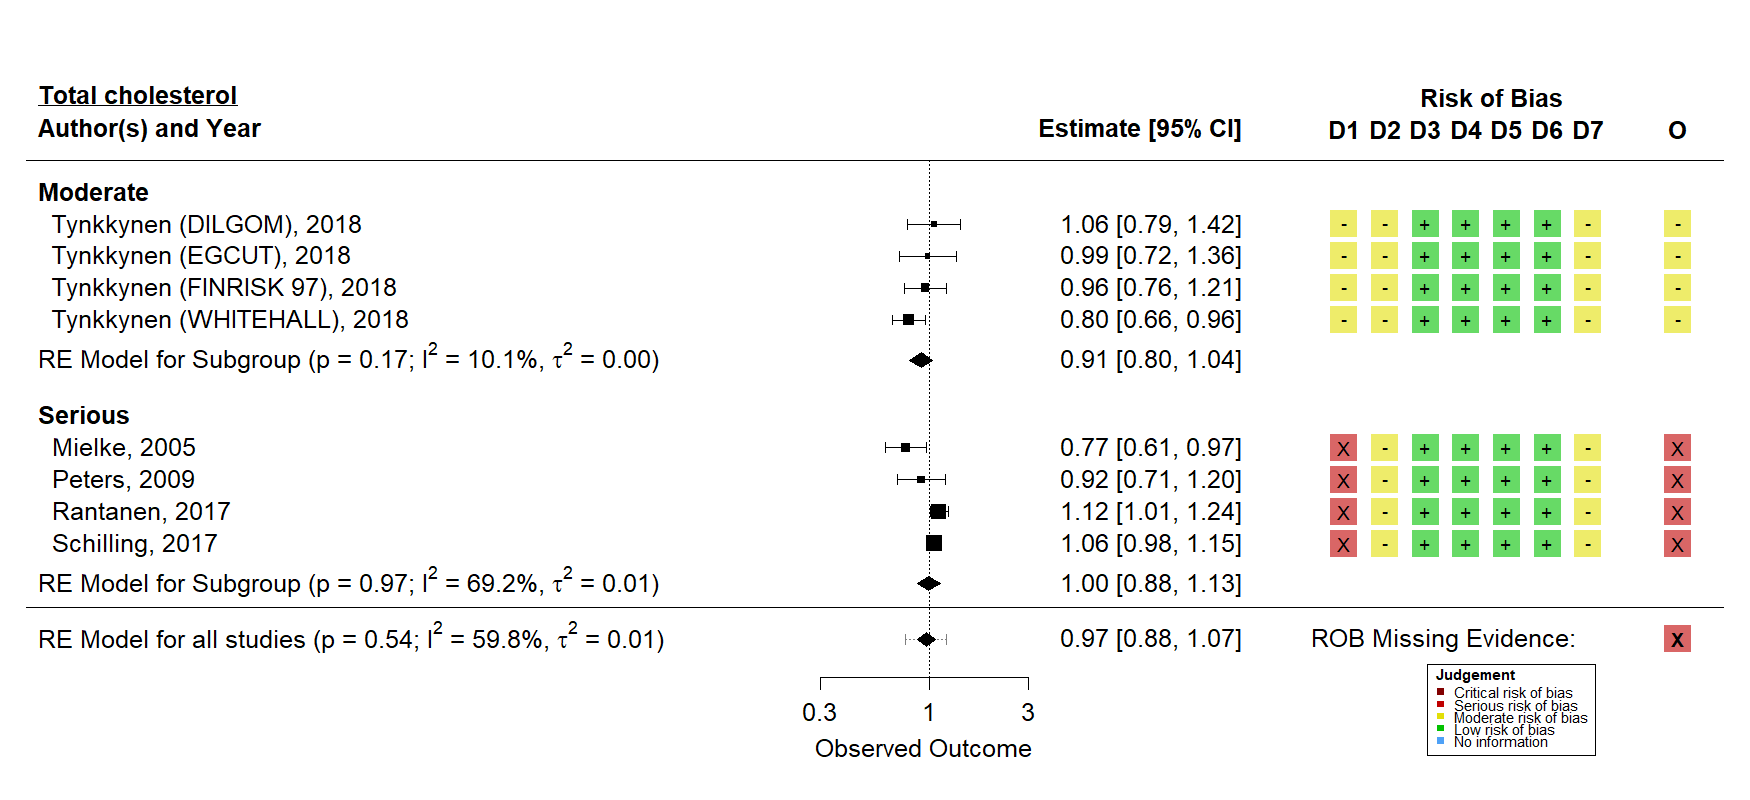
\includegraphics[width=1\linewidth]{figures/sys-rev/fp_obs_Dementia_TC_}

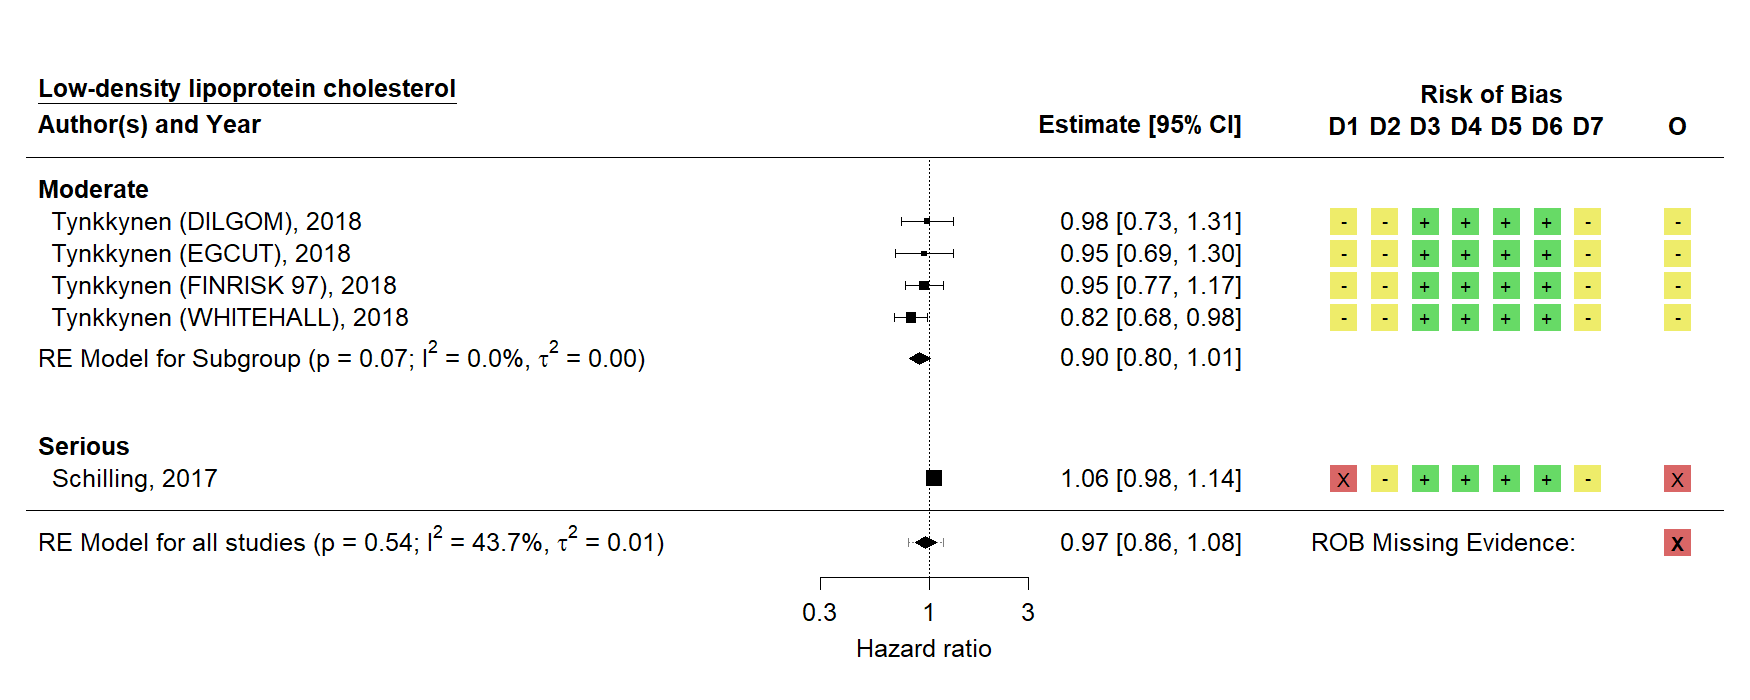
\includegraphics[width=1\linewidth]{figures/sys-rev/fp_obs_Dementia_LDL_}

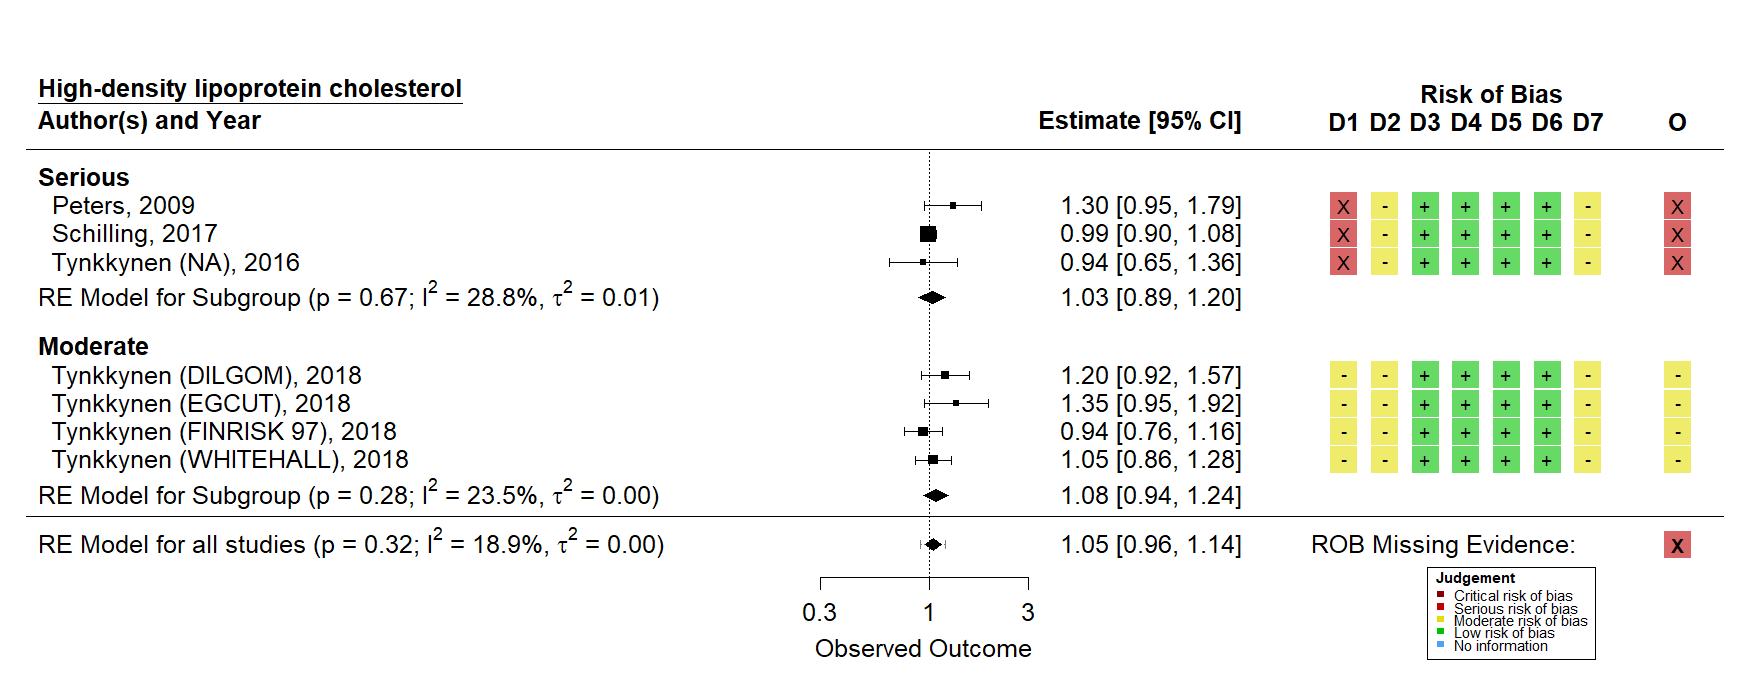
\includegraphics[width=1\linewidth]{figures/sys-rev/fp_obs_Dementia_HDL_}

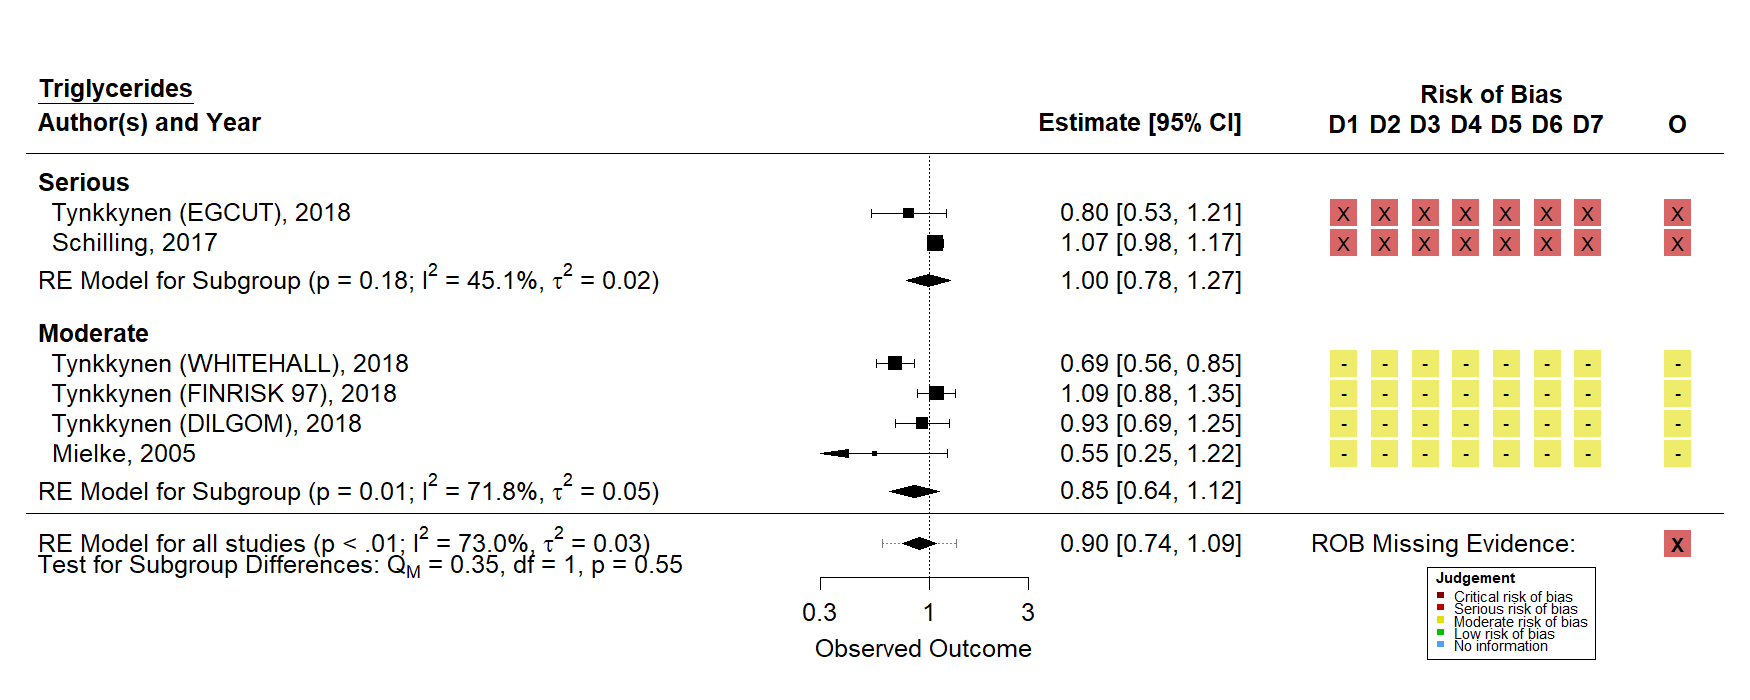
\includegraphics[width=1\linewidth]{figures/sys-rev/fp_obs_Dementia_TG_}





\begin{longtable}[t]{>{\raggedright\arraybackslash}p{6.4em}>{\raggedright\arraybackslash}p{6.4em}>{\raggedright\arraybackslash}p{6.4em}>{\raggedright\arraybackslash}p{6.4em}>{\raggedright\arraybackslash}p{6.4em}}
\caption[Mendelian randomisation risk-of-bias assessment tool]{\label{tab:mrTool-table}Tool used to assess risk of bias in Mendelian randomisation studies, adapted from that developed by Mamluk et al.\textsuperscript{\protect\hyperlink{ref-mamluk2020}{149}}}\\
\toprule
\textbf{Bias domain} & \textbf{Question} & \textbf{High} & \textbf{Moderate} & \textbf{Low}\\
\midrule
\endfirsthead
\caption[]{\label{tab:mrTool-table}Tool used to assess risk of bias in Mendelian randomisation studies, adapted from that developed by Mamluk et al.\textsuperscript{\protect\hyperlink{ref-mamluk2020}{149}} \textit{(continued)}}\\
\toprule
\textbf{Bias domain} & \textbf{Question} & \textbf{High} & \textbf{Moderate} & \textbf{Low}\\
\midrule
\endhead

\endfoot
\bottomrule
\endlastfoot
Weak instrument bias & Strength of association between instrument and exposure F statistic < 10 in the same sample  (< 10 indicating a weak instrument) & F<10 & F= missing or F\textasciitilde{}10 & F>>10\\
\midrule
Genetic confounding bias & Reported test on association between confounders and IV (testing the assumption that the instrument is associated with your outcome only via your exposure) & Yes AND there is an obvious association & Not presented or 
Yes presented AND there is some degree of association & Presented and no obvious association\\
\midrule
‘Other’ Confounding bias & Included confounders in the IV analysis & Yes &  & No\\
\midrule
Additional direct effects between IV and outcome (exclusion restriction assumption) & Presence of pleiotropy for genetic IVs & Genetic IVs with no knowledge of mechanism for G-lipid association (e.g. GWAS hit, could be acting through any pathway…) & Biologically plausible lipid-specific mechanism of association for G-lipid (e.g. lipid metabolising genetic variants) & Same as moderate AND checks that there is no other known effect of genetic variants on outcome or its risk-factors\\
\midrule
Bias due to selection of participants & Homogenous population or similar ancestry 
If no: Stratified by ethnicity or adjusted for population stratification (yes/no) & Non-homogenous population (e.g. black and white together, etc.) & Population described as homogenous (e.g. whites only) BUT not corrected for ancestry informative markers like principal components derived from GWAS &  Population described as homogenous (e.g. whites only) AND corrected for ancestry informative markers like principal components derived from GWAS\\*
\end{longtable}

\hypertarget{appendix-cprd-analysis}{%
\section{Chapter \ref{cprd-analysis-heading}}\label{appendix-cprd-analysis}}

\hypertarget{appendix-cprd-amendments}{%
\subsection{Amendments to protocol}\label{appendix-cprd-amendments}}

\hypertarget{code-lists}{%
\subsection{Code lists}\label{code-lists}}

\hypertarget{appendix-ipd-analysis}{%
\section{Chapter \ref{ipd-heading}}\label{appendix-ipd-analysis}}

\hypertarget{ipd-email-collab}{%
\subsection{Email and documents sent to potental collaborators}\label{ipd-email-collab}}

\hypertarget{section-2}{%
\subsection{Section 2}\label{section-2}}

\hypertarget{chapter-refdiscussion-heading}{%
\section{Chapter \ref{discussion-heading}}\label{chapter-refdiscussion-heading}}

\hypertarget{catalogue-of-failures}{%
\subsection{Catalogue of failures}\label{catalogue-of-failures}}

Short section detailing the things I tried to do but which did not work.

\hypertarget{other-appendix-heading}{%
\chapter{Other Appendix}\label{other-appendix-heading}}

\hypertarget{software-used-to-create-this-thesis}{%
\section{Software used to create this thesis}\label{software-used-to-create-this-thesis}}

This thesis was written in RMarkdown. Several R packages were used as part of this project.\textsuperscript{\protect\hyperlink{ref-R-base}{\textbf{R-base?}},\protect\hyperlink{ref-R-bookdown}{\textbf{R-bookdown?}},\protect\hyperlink{ref-R-dagitty}{\textbf{R-dagitty?}},\protect\hyperlink{ref-R-data.table}{\textbf{R-data.table?}},\protect\hyperlink{ref-R-DiagrammeR}{\textbf{R-DiagrammeR?}},\protect\hyperlink{ref-R-dplyr}{\textbf{R-dplyr?}},\protect\hyperlink{ref-R-flextable}{\textbf{R-flextable?}},\protect\hyperlink{ref-R-ggdag}{\textbf{R-ggdag?}},\protect\hyperlink{ref-R-ggplot2}{\textbf{R-ggplot2?}},\protect\hyperlink{ref-R-kableExtra}{\textbf{R-kableExtra?}},\protect\hyperlink{ref-R-knitr}{\textbf{R-knitr?}},\protect\hyperlink{ref-R-koRpus}{\textbf{R-koRpus?}},\protect\hyperlink{ref-R-koRpus.lang.en}{\textbf{R-koRpus.lang.en?}},\protect\hyperlink{ref-R-magrittr}{\textbf{R-magrittr?}},\protect\hyperlink{ref-R-Matrix}{\textbf{R-Matrix?}},\protect\hyperlink{ref-R-medrxivr}{\textbf{R-medrxivr?}},\protect\hyperlink{ref-R-metafor}{\textbf{R-metafor?}},\protect\hyperlink{ref-R-networkD3}{\textbf{R-networkD3?}},\protect\hyperlink{ref-R-patchwork}{\textbf{R-patchwork?}},\protect\hyperlink{ref-R-png}{\textbf{R-png?}},\protect\hyperlink{ref-R-readxl}{\textbf{R-readxl?}},\protect\hyperlink{ref-R-robvis}{\textbf{R-robvis?}},\protect\hyperlink{ref-R-sf}{\textbf{R-sf?}},\protect\hyperlink{ref-R-sylly}{\textbf{R-sylly?}},\protect\hyperlink{ref-bookdown2016}{\textbf{bookdown2016?}},\protect\hyperlink{ref-dagitty2016}{\textbf{dagitty2016?}},\protect\hyperlink{ref-ggplot22016}{\textbf{ggplot22016?}},\protect\hyperlink{ref-knitr2015}{\textbf{knitr2015?}},\protect\hyperlink{ref-knitr2014}{\textbf{knitr2014?}},\protect\hyperlink{ref-koRpus2018}{\textbf{koRpus2018?}},\protect\hyperlink{ref-koRpus.lang.en2019}{\textbf{koRpus.lang.en2019?}},\protect\hyperlink{ref-medrxivr2020}{\textbf{medrxivr2020?}},\protect\hyperlink{ref-metafor2010}{\textbf{metafor2010?}},\protect\hyperlink{ref-robvis2020}{\textbf{robvis2020?}},\protect\hyperlink{ref-sf2018}{\textbf{sf2018?}},\protect\hyperlink{ref-sylly2018}{\textbf{sylly2018?}}}
All projects in these thesis attempt to conform to minimal best practices for research computing.\textsuperscript{\protect\hyperlink{ref-wilson2014}{328},\protect\hyperlink{ref-wilson2017}{329}}

\hypertarget{appendix-robvis}{%
\section{\texorpdfstring{Producing risk-of-bias visualisations with \texttt{robvis}}{Producing risk-of-bias visualisations with robvis}}\label{appendix-robvis}}

\hypertarget{introduction-3}{%
\subsection{Introduction}\label{introduction-3}}

Risk of bias assessment - evaluation of the internal validity of studies included in a systematic review - often forms a key part of the evidence synthesis process, particularly in the health sciences.\textsuperscript{\protect\hyperlink{ref-cochranechpt7}{\textbf{cochranechpt7?}}} A well-developed family of tools is widely used, which have in common the characteristic that they evaluate specific domains of bias rather being constructed as a checklist or a quantitative score.\textsuperscript{\protect\hyperlink{ref-cochranechpt7}{\textbf{cochranechpt7?}}} These tools include the RoB 2 tool for randomized trials,\textsuperscript{\protect\hyperlink{ref-sterne2019rob}{\textbf{sterne2019rob?}}} the ROBINS-I tool for non-randomized studies of interventions,\textsuperscript{\protect\hyperlink{ref-sterne2016}{142}} the QUADAS 2 tool for test accuracy and the ROBIS tool for systematic reviews.\textsuperscript{\protect\hyperlink{ref-whiting2011quadas}{\textbf{whiting2011quadas?}}} Within each bias domains a judgement is reached about the strength of the study in that regard: for example, the first domain in the Cochrane RoB 2 tool deals with bias arising from the randomization process.\textsuperscript{\protect\hyperlink{ref-sterne2019rob}{\textbf{sterne2019rob?}}} Accessible graphics summarizing the results of these domain-based risk-of-bias assessments are included in reports of systematic reviews. A convenient plot in many reviews is a ``traffic light'' plot, which tabulates the judgement for each study in each domain. For larger numbers of studies, when such a table become unmanageable, a popular alternative is a weighted bar plot, which show the proportion of information with each judgement for each domain.\textsuperscript{\protect\hyperlink{ref-higgins2008assessing}{\textbf{higgins2008assessing?}}}

Researchers can face a number of barriers in creating these plots. While some evidence synthesis platforms, such as Cochrane's Review Manager,\textsuperscript{\protect\hyperlink{ref-cochrane2014review}{\textbf{cochrane2014review?}}} are able to produce these visualizations, not all researchers use these systems to conduct their systematic reviews, and copying the risk-of-bias data into these systems simply to produce the plots is inefficient and error prone. Likewise, creating the figures by hand, through software such as MS PowerPoint or Adobe Illustrator, may lead to unintentional errors and require the plots to be redrawn during an update to the review. Additionally, while the field of evidence synthesis software has grown rapidly in recent years,\textsuperscript{\protect\hyperlink{ref-marshall2015systematic}{\textbf{marshall2015systematic?}}} this growth has not been equally distributed across the different aspects of the systematic review process. For example, a recent review found several software offerings aimed specifically at the abstract screening stage of the review process,\textsuperscript{\protect\hyperlink{ref-harrison2020software}{\textbf{harrison2020software?}}} but no similar time- and error-reducing tool has been proposed for visualizing the results of risk-of-bias assessments.

Fortunately, tools such as R, RStudio and \texttt{Shiny} (an R package for building interactive web apps) have made it easier than ever to produce such a tool.\textsuperscript{\protect\hyperlink{ref-rref}{\textbf{rref?}},\protect\hyperlink{ref-rstudioref}{\textbf{rstudioref?}},\protect\hyperlink{ref-shinyref}{\textbf{shinyref?}}} Here, we present \texttt{robvis} (Risk Of Bias VISualiation),\textsuperscript{\protect\hyperlink{ref-mcguinness2019a}{\textbf{mcguinness2019a?}}} an R package and \texttt{Shiny} web-app that allows users to create publication-ready risk-of-bias plots quickly and easily. Originally created for use with the major risk-of-bias assessment tools used in health research, the tool allows users to visualize the results from any domain-based risk-of-bias assessment or quality appraisal tool.

The tool is open-source and available to use free of charge. Users can download a stable version of the R package from CRAN (\url{https://cran.r-project.org/package=robvis}); or access and contribute to the development version via GitHub (\url{https://github.com/mcguinlu/robvis}).

\hypertarget{development-1}{%
\subsection{Development}\label{development-1}}

Development of \texttt{robvis} began in April 2019 at the Evidence Synthesis Hackathon (ESH), an event which brings together interested researchers, practitioners and coders to discuss and develop new open-source evidence synthesis technologies. Test versions of both the R package and the web app were made available in early June 2019, with attendees of the ESH and members of the Bristol Appraisal and Review of Research (BARR) group at the University of Bristol being invited to test the tool and provide feedback. This feedback, along with other feature suggestions from the wider evidence synthesis community captured via GitHub issues, was incorporated and the first release version of the package was uploaded to CRAN in November 2019. The tool has been well received and is beginning to be cited in the evidence synthesis literature.\textsuperscript{\protect\hyperlink{ref-simillis2020}{330},\protect\hyperlink{ref-tanneru2020}{331},\protect\hyperlink{ref-gibb2019consistent}{\textbf{gibb2019consistent?}},\protect\hyperlink{ref-habadi2019prevalence}{\textbf{habadi2019prevalence?}},\protect\hyperlink{ref-veloso2020effectiveness}{\textbf{veloso2020effectiveness?}}}

\hypertarget{installation-1}{%
\subsection{Installation}\label{installation-1}}

A stable version of \texttt{robvis} is hosted on the Comprehensive R Archive Network (CRAN) and can be installed using:

\begin{Shaded}
\begin{Highlighting}[]
\FunctionTok{install.packages}\NormalTok{(}\StringTok{"robvis"}\NormalTok{)}
\end{Highlighting}
\end{Shaded}

As development of \texttt{robvis} is ongoing, new features are often available in the development version some time before they appear in the stable CRAN version. The most recent development version can be install from GitHub using:

\begin{Shaded}
\begin{Highlighting}[]
\NormalTok{devtools}\SpecialCharTok{::}\FunctionTok{install\_github}\NormalTok{(}\StringTok{"mcguinlu/robvis"}\NormalTok{)}
\end{Highlighting}
\end{Shaded}

\hypertarget{usage-1}{%
\subsection{Usage}\label{usage-1}}

\texttt{robvis} contains two main functions. The first, \texttt{rob\_traffic\_light()}, creates a traffic light plot by tabulating each study by each domain, providing a more detailed view of the results of the risk-of-bias assessment. The second, \texttt{rob\_summary()}, creates a weighted bar plot showing the proportion of information with each judgement for each domain in the assessment tool specified.

A worked example using these functions is outlined below, showing the ease with which risk-of-bias plots can be created using \texttt{robvis}. A detailed description of the additional options that can be used with each function is presented in Table \ref{tab:robvisarguments}

Using the example data set (\texttt{data\_rob2}) which is built into the package and is presented in Table \ref{tab:robdata} for reference, the traffic light plot shown in Figure \ref{fig:trafficplot} is created using:

\begin{Shaded}
\begin{Highlighting}[]
\FunctionTok{rob\_traffic\_light}\NormalTok{(}\AttributeTok{data =}\NormalTok{ data\_rob2,}
                  \AttributeTok{tool =} \StringTok{"ROB2"}\NormalTok{,}
                  \AttributeTok{psize =} \DecValTok{15}\NormalTok{)}
\end{Highlighting}
\end{Shaded}

\begin{figure}
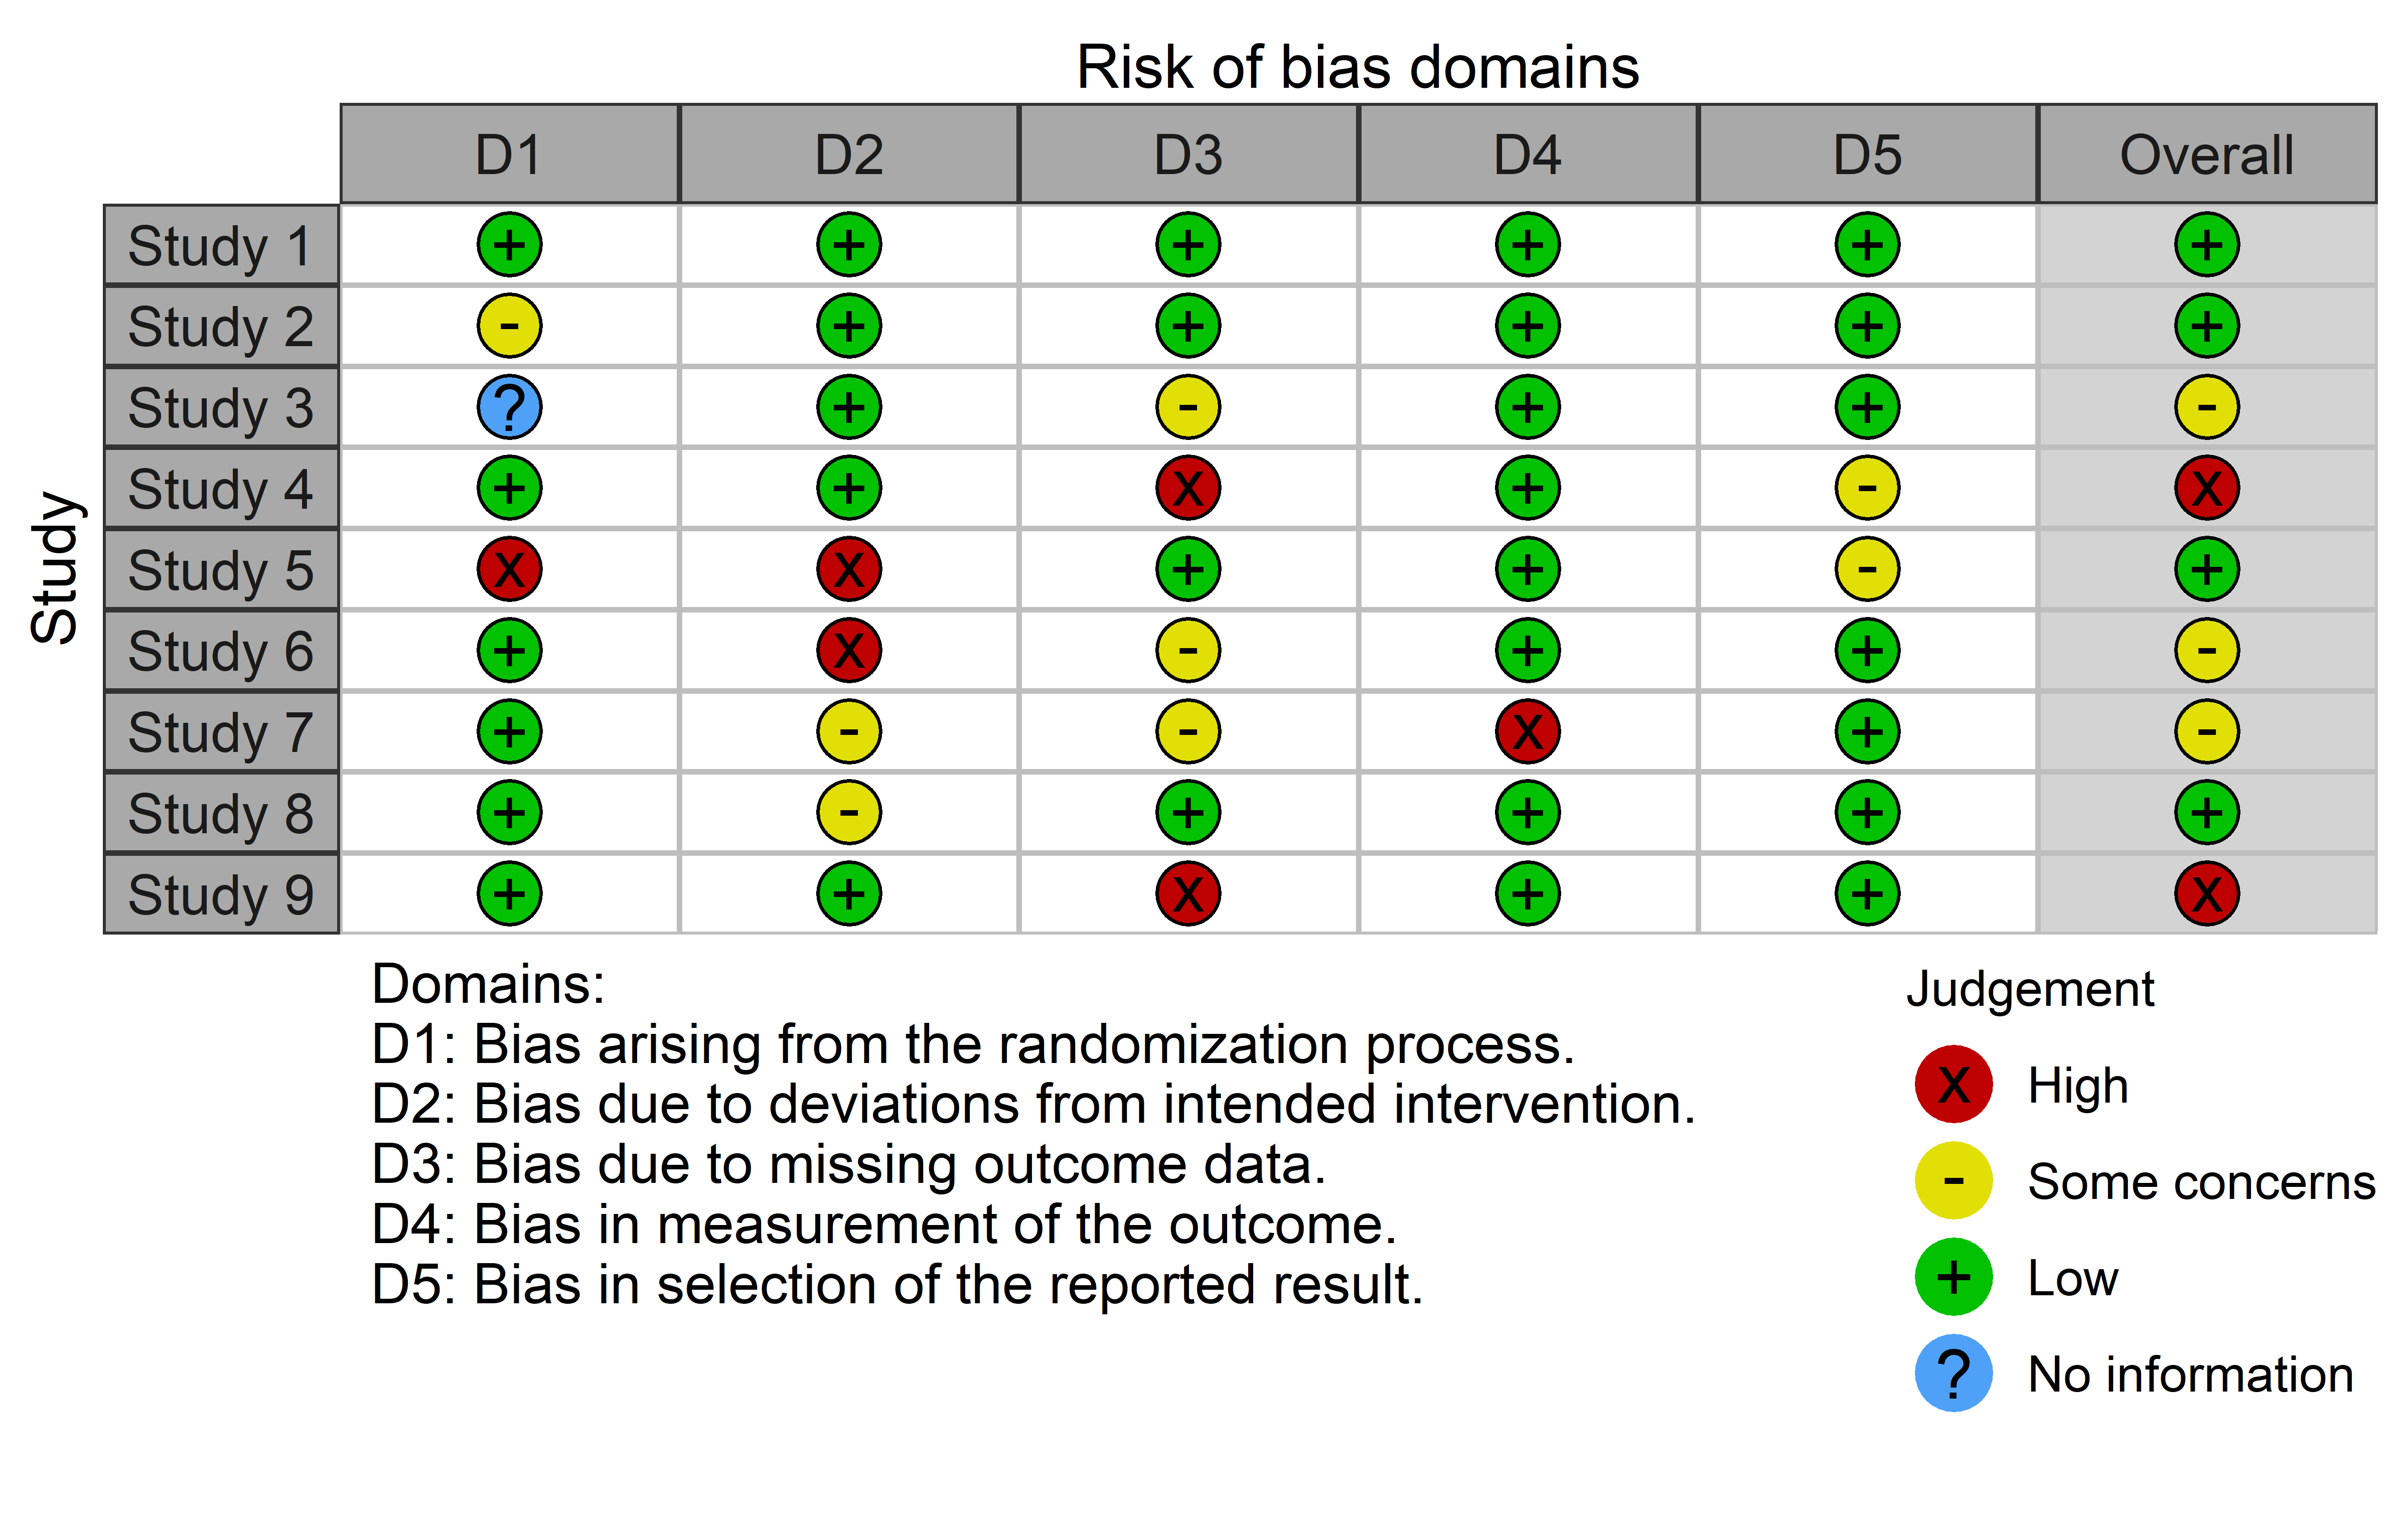
\includegraphics[width=1\linewidth]{figures/sys-rev-tools/example-rob-traffic-light-plot} \caption{Example risk of bias traffic light plot created using `robvis`}\label{fig:trafficplot}
\end{figure}

Similary, using the same data set, the summary barplot shown in Figure \ref{fig:summaryplot} is created using:

\begin{Shaded}
\begin{Highlighting}[]
\FunctionTok{rob\_summary}\NormalTok{(}\AttributeTok{data =}\NormalTok{ data\_rob2,}
            \AttributeTok{tool =} \StringTok{"ROB2"}\NormalTok{, }
            \AttributeTok{overall =} \ConstantTok{TRUE}\NormalTok{)}
\end{Highlighting}
\end{Shaded}

\begin{figure}
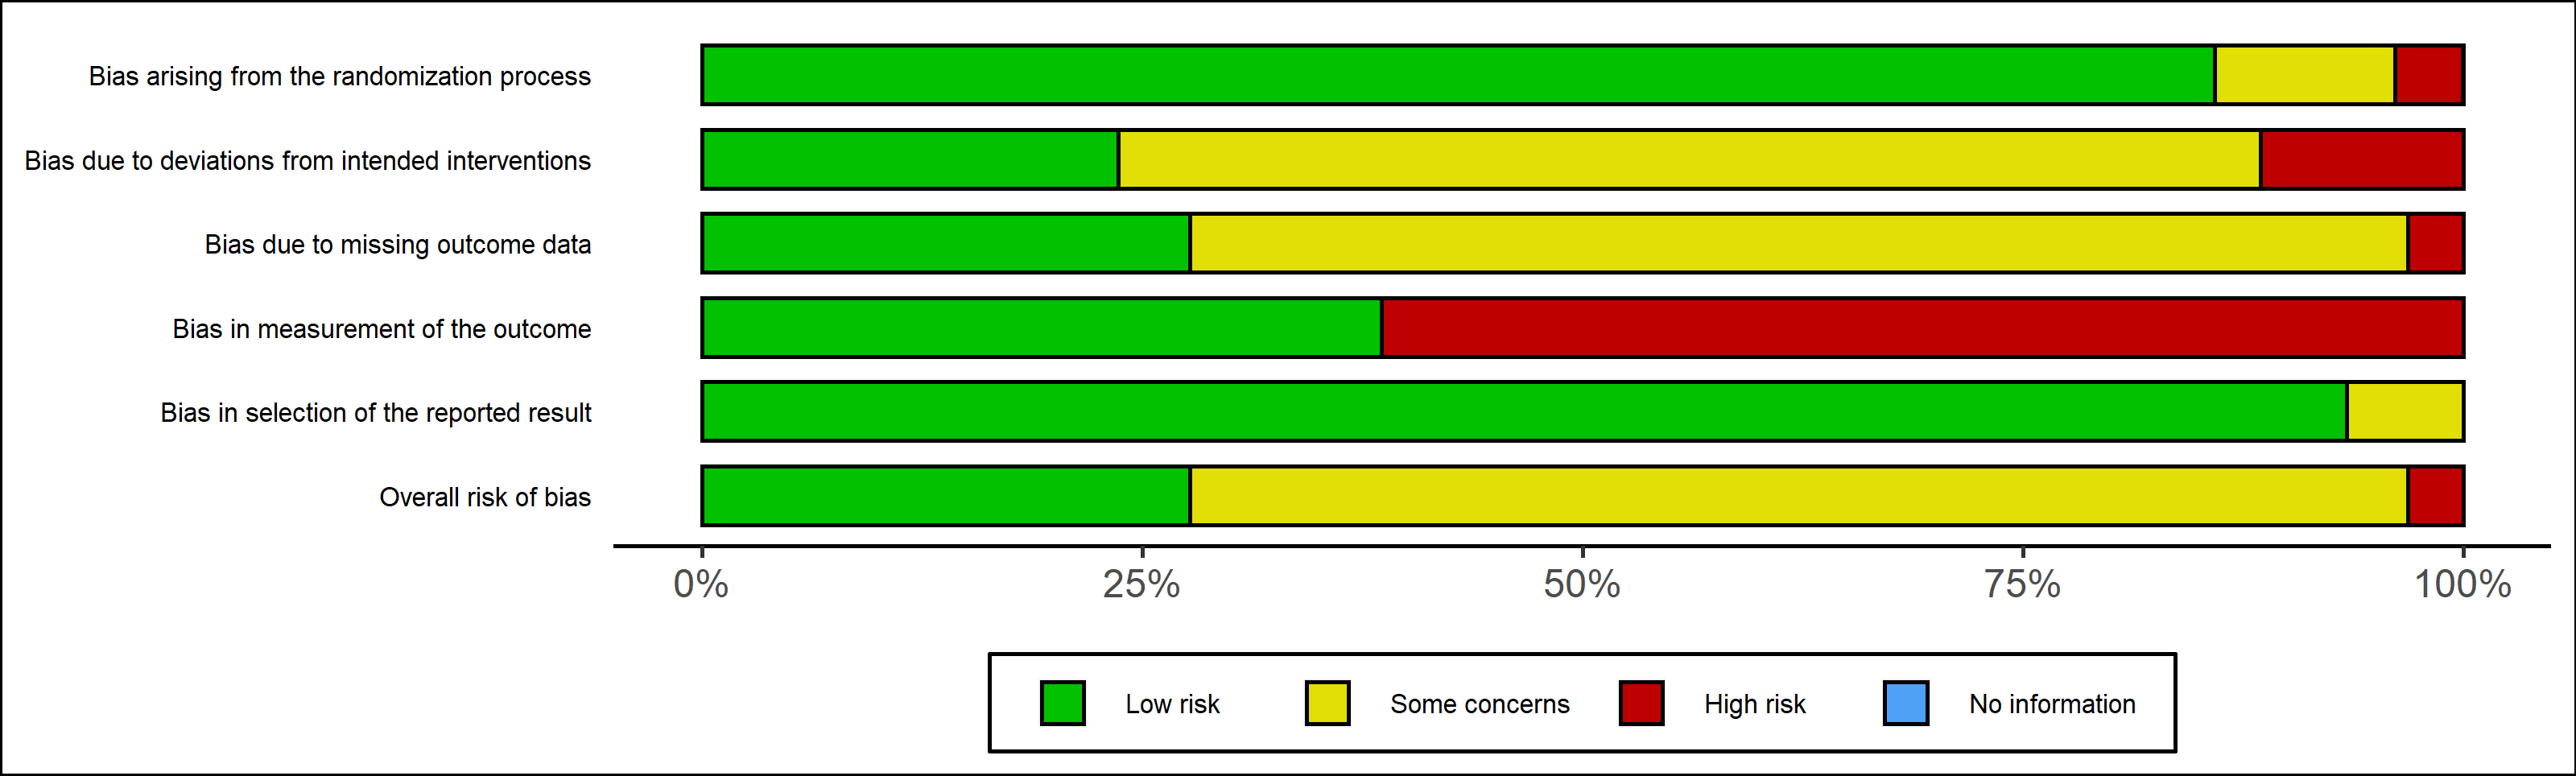
\includegraphics[width=1\linewidth]{figures/sys-rev-tools/example-rob-summary-barplot} \caption{Example risk of bias summary plot created using `robvis` and the example ROB2 dataset}\label{fig:summaryplot}
\end{figure}

A list of arguments available to the two functions in robvis are shown in Table \ref{tab:robvisarguments}

~

\begingroup\fontsize{9}{11}\selectfont

\begin{longtable}[t]{lcc>{\raggedright\arraybackslash}p{5cm}}
\caption{\label{tab:robvisarguments}Description of the arguments available in the two main `robvis` functions. ‘X’ indicates that the option is available for the respective function.}\\
\toprule
Argument & rob\_traffic\_light() & rob\_summary() & Description\\
\midrule
\endfirsthead
\caption[]{\label{tab:robvisarguments}Description of the arguments available in the two main `robvis` functions. ‘X’ indicates that the option is available for the respective function. \textit{(continued)}}\\
\toprule
Argument & rob\_traffic\_light() & rob\_summary() & Description\\
\midrule
\endhead

\endfoot
\bottomrule
\endlastfoot
\cellcolor{gray!6}{data} & \cellcolor{gray!6}{X} & \cellcolor{gray!6}{X} & \cellcolor{gray!6}{Defines the dataframe containing the summary (domain) level risk-of-bias assessments. See the text and Table 1 for the format expected by `robvis`}\\
tool & X & X & Defines the risk of bias assessment tool used. The RoB2 (`tool="ROB2"`), ROBINS-I (`tool="ROBINS-I"`), and QUADAS-2 (`tool="QUADAS-2"`) assessments tools are currently supported. Other tools can be visualised using the generic template (`tool = "Generic"`)\\
\cellcolor{gray!6}{colour} & \cellcolor{gray!6}{X} & \cellcolor{gray!6}{X} & \cellcolor{gray!6}{Defines the colour scheme for the plot. The default is `colour = "cochrane"` which uses the "Cochrane" (red, yellow, green) colours, while a preset option for a colour-blind friendly palette is also available (`colour = "colourblind"`). Alternatively, users can specify their own colour scheme e.g. `colour = c("\#f442c8", "\#bef441", "\#000000")`}\\
overall &  & X & Defines whether to include an additional bar showing the distibution of overall risk of bias judgements in the summary barplot figure. Default is `overall = FALSE`.\\
\cellcolor{gray!6}{weighted} & \cellcolor{gray!6}{} & \cellcolor{gray!6}{X} & \cellcolor{gray!6}{Defines whether weights should be used to produce the summary barplot figure. Default is `weighted = TRUE`, in line with current Cochrane Collaboration guidance.}\\
\addlinespace
psize & X &  & Defines the size of the points in the traffic light plot. Default is `psize = 20`.\\*
\end{longtable}
\endgroup{}

~

\hypertarget{reception-and-future-plans-1}{%
\subsection{Reception and Future Plans}\label{reception-and-future-plans-1}}

As of December 2021, \texttt{robvis} has been downloaded more than 15800 times. It has been well received but the systematic review community, and has been cited frequently in the published literature. A paper describing the tool was published in a special issue of Research Synthesis Methods focusing on data visualisation methods. A chapter on the tool has been incorporated in to the ``Doing Meta-Analysis in R'' online textbook.\textsuperscript{\protect\hyperlink{ref-mathias_harrer_2019_2551803}{\textbf{mathias\_harrer\_2019\_2551803?}}}

While \texttt{robvis} is a stable package, a range of additional functionality could be added. At present, the number of tools with a specific template included in \texttt{robvis} is limited - adding additional templates is a priority. For example, a template for ROBIS, a tool for assessing risk of bias in systematic reviews, is in developement.\textsuperscript{\protect\hyperlink{ref-whiting2016robis}{\textbf{whiting2016robis?}}} Additionally, the tool does not yet allow for the production of paired forest plots, where the risk-of-bias judgement is presented alongside each specific result included in the meta-analysis.\textsuperscript{\protect\hyperlink{ref-cochranechpt7}{\textbf{cochranechpt7?}}} This was initially considered to be beyond the scope of the tool, as it involves the visualization of something other than risk-of-bias assessments. However, following user-driven demand, this functionality is in development and will be available in the near future. Finally, we would like to add similar functionality to that provided by the \texttt{metafor::reporter()} function, which generates a brief paragraph of text describing the results of a meta-analysis. The future \texttt{robvis::reporter()} function would provide a boilerplate description of the assessment tool used and the key domains at risk of bias.

\hypertarget{creating}{%
\section{Creating}\label{creating}}

\newpage

\hypertarget{published-papers}{%
\section{Copies of papers arising from this thesis}\label{published-papers}}

The following pages contain copies of papers arising from work performed as part of this thesis.

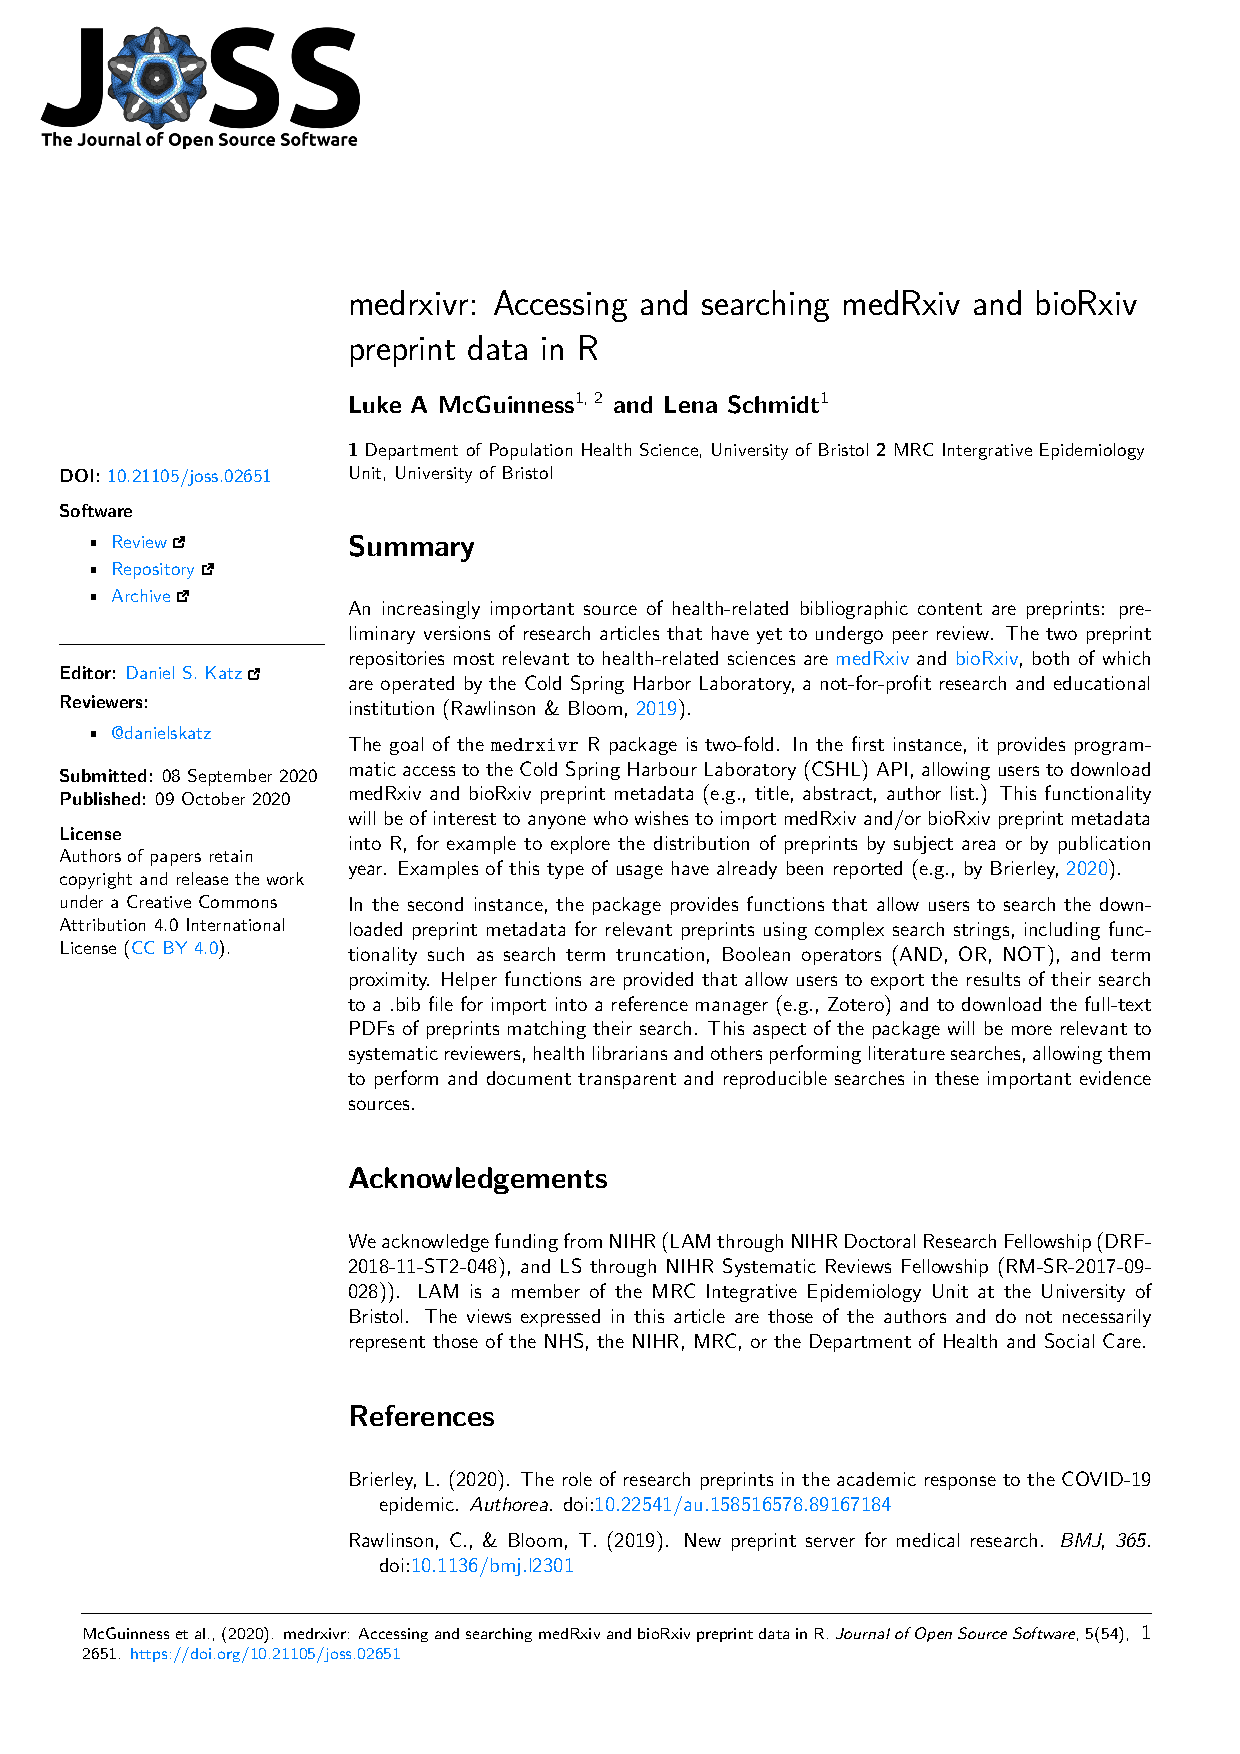
\includepdf[pages=-,pagecommand={\thispagestyle{empty}}]{published/medrxivr.pdf}
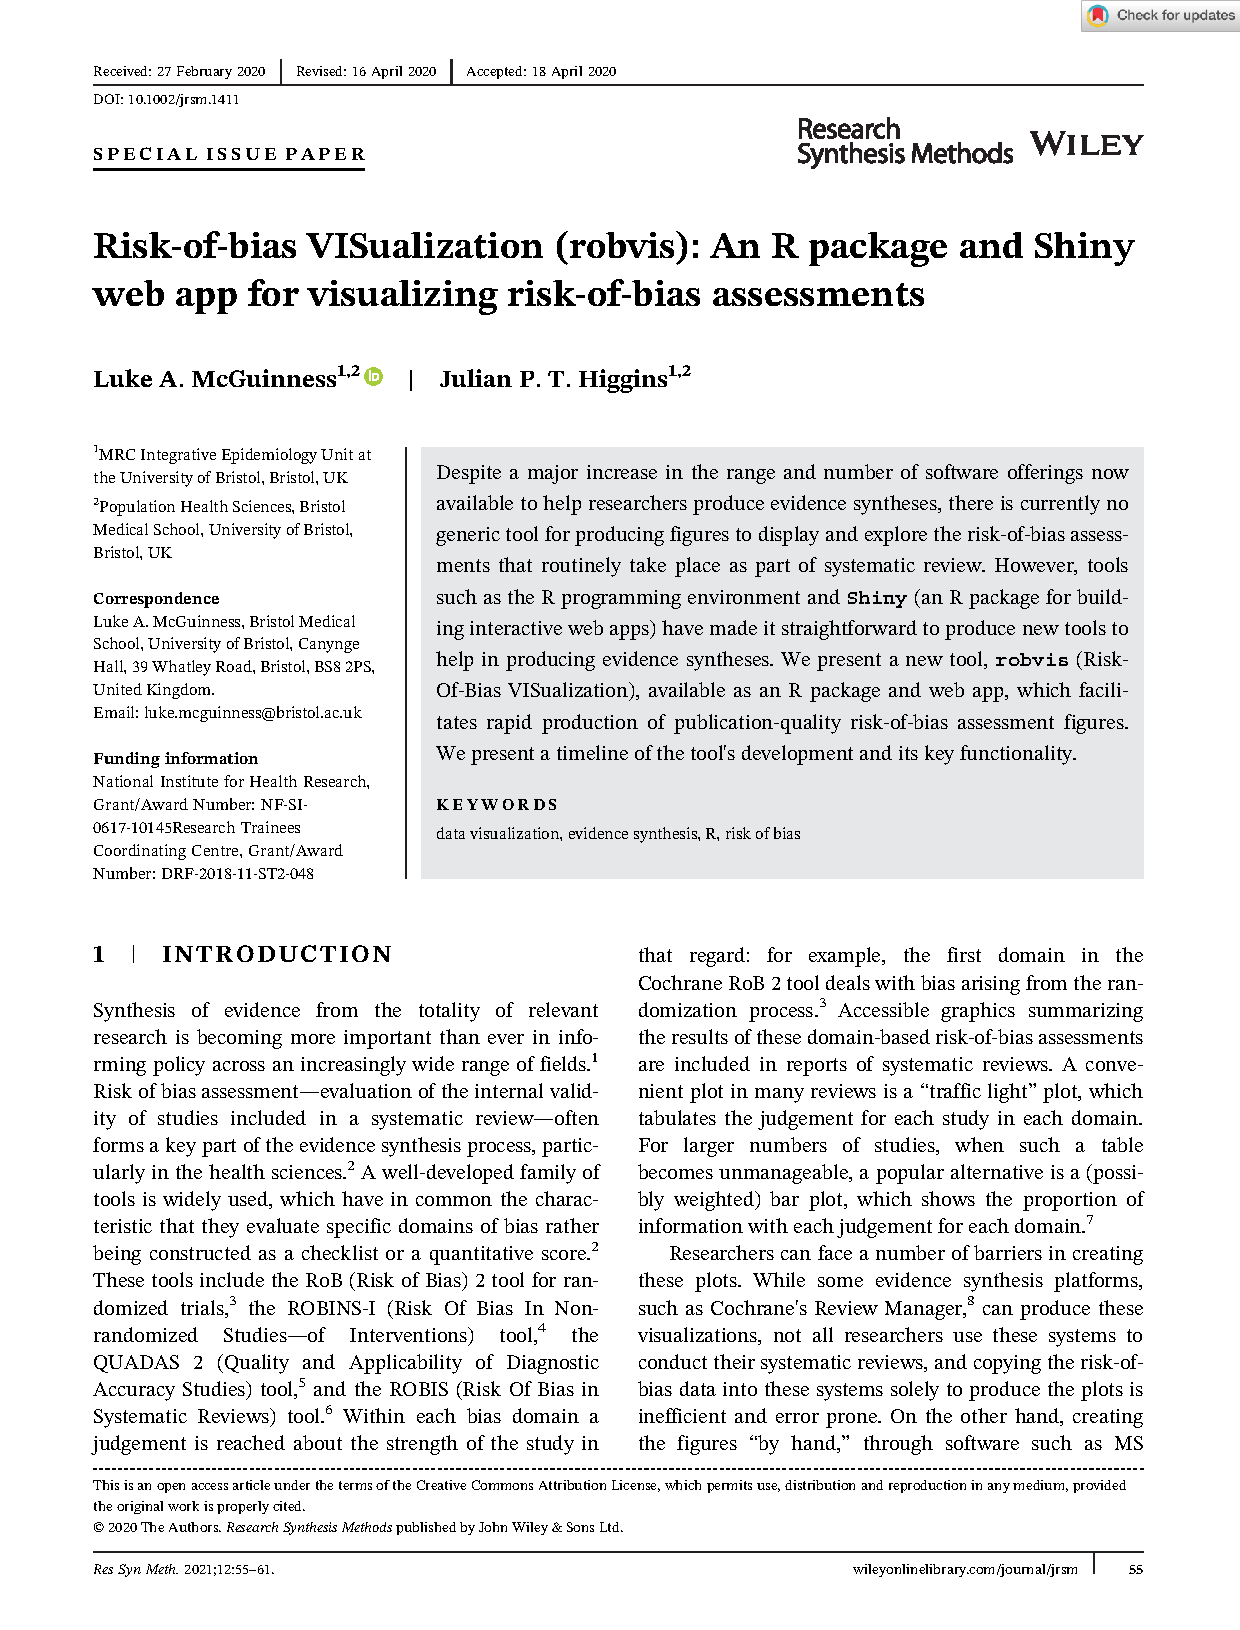
\includepdf[pages=-,pagecommand={\thispagestyle{empty}}]{published/robvis.pdf}
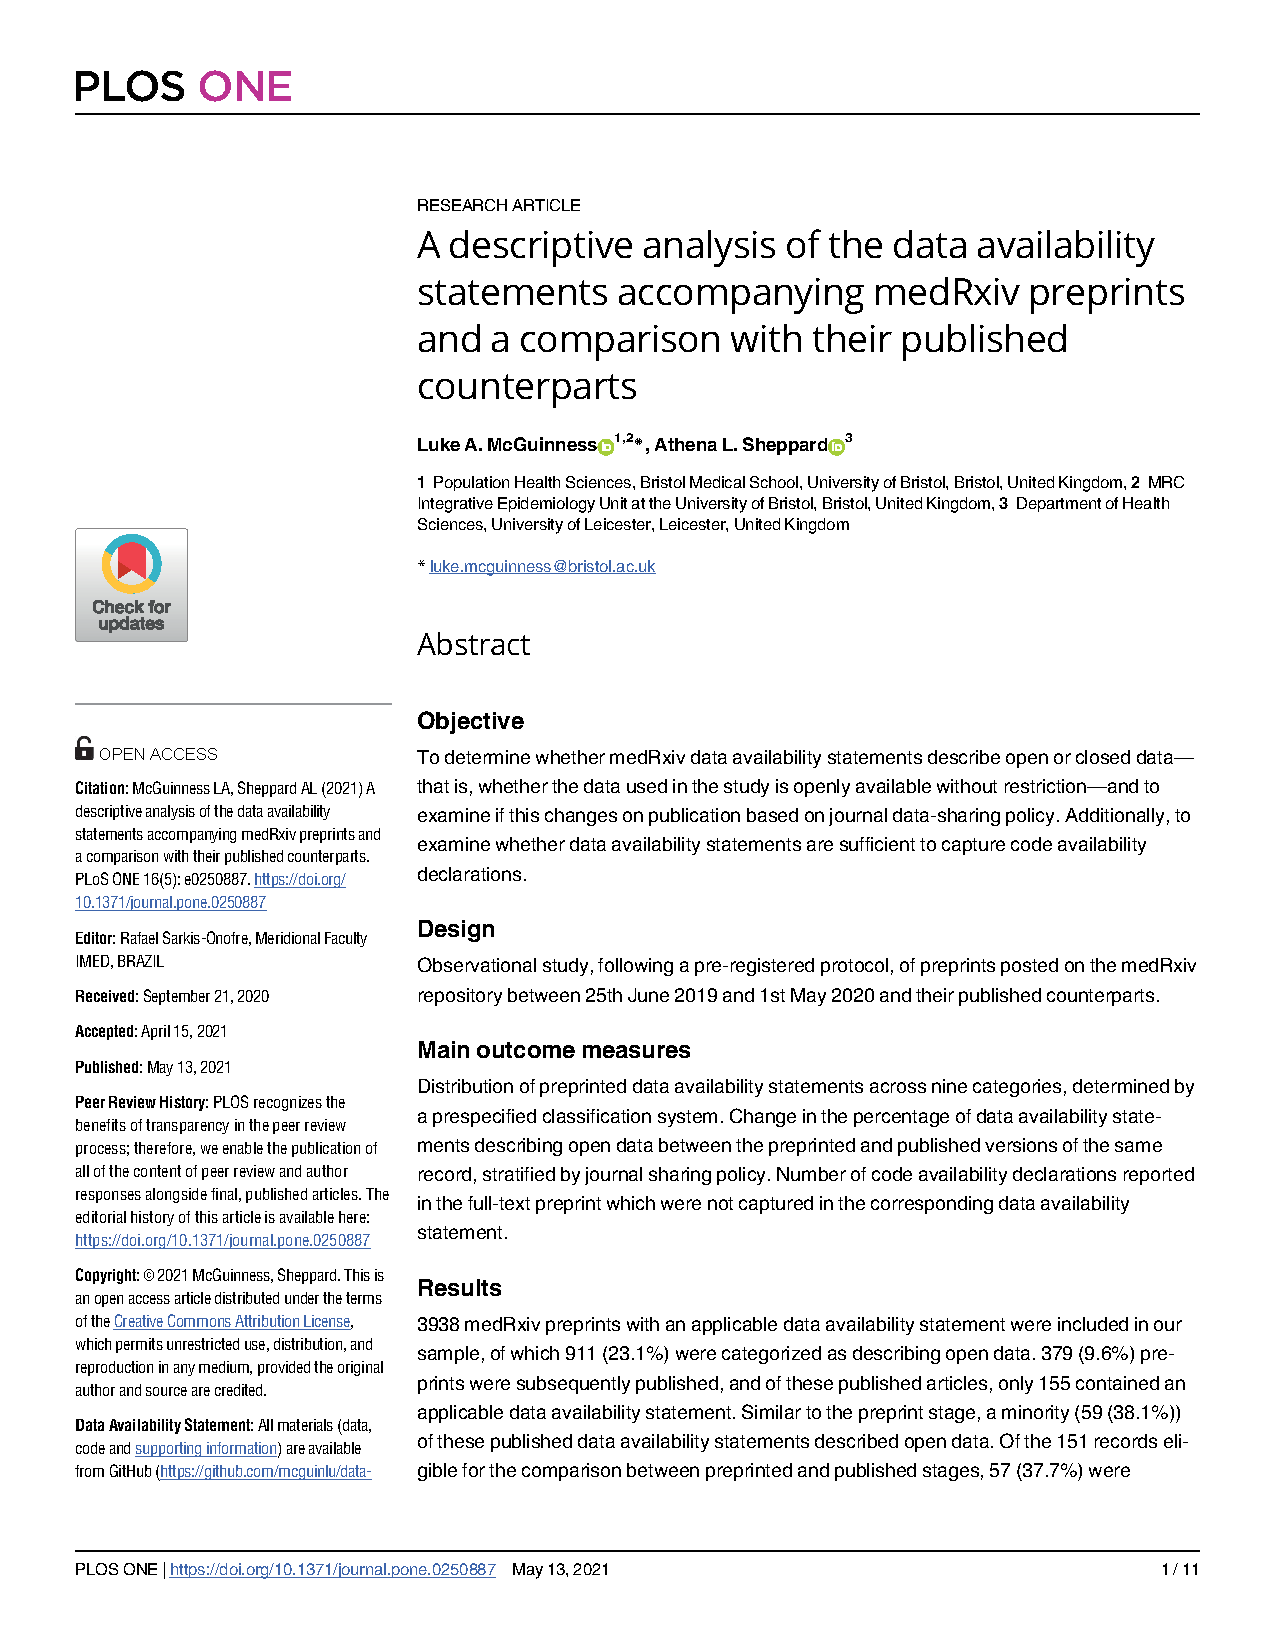
\includepdf[pages=-,pagecommand={\thispagestyle{empty}}]{published/DAS_comparison.pdf}
\includepdf[pages=-,pagecommand={\thispagestyle{empty}}]{published/prevsci.pdf}

%%%%% REFERENCES

\setlength{\baselineskip}{0pt} % JEM: Single-space References

{\renewcommand*\MakeUppercase[1]{#1}%
\printbibliography[heading=bibintoc,title={\bibtitle}]}

\end{document}
